\documentclass[11pt,oneside]{article}
\usepackage[paperwidth=6.5in,paperheight=9.5in,margin=.6in]{geometry}
\usepackage{fontspec}
\setmainfont{lmroman10-regular.otf}[BoldFont=lmroman10-bold.otf,ItalicFont=lmroman10-italic.otf,BoldItalicFont=lmroman10-bolditalic.otf,SmallCapsFont=lmromancaps10-regular.otf]
\usepackage[german]{babel}
\germansetup{glottonyms=legacy,hyphenrules=legacy}
\usepackage{amsmath,amssymb,microtype,needspace,graphicx,tikz}
\usepackage[unicode,hidelinks,hyperfootnotes=false]{hyperref}
\hypersetup{pdftitle={Gauss Werke Band VIII: Titelblätter; Arithmetik und Algebra; elf Abhandlungen zur Analysis},pdfauthor={}}
\newcommand{\BareRoot}[1]{\mathord{\surd}#1}
\newcommand{\SourceLeaf}[1]{\hypertarget{native-#1}{}}
\newcommand{\HistoricalNote}[3]{#1\begingroup\renewcommand{\thefootnote}{#2}\footnotetext{#3}\endgroup}
\makeatletter
\long\def\@makefntext#1{\parindent1em\noindent\hb@xt@2.4em{\hss\@thefnmark\ }#1}
\makeatother
\setlength{\parindent}{1.2em}
\setlength{\emergencystretch}{1.4em}
\widowpenalty=10000\clubpenalty=10000\raggedbottom
\begin{document}
% Modern GDZ wrapper outside the historical body; complete private reading retained.

\SourceLeaf{2}
\thispagestyle{empty}
\begin{center}
\vspace*{1em}
{\Large CARL FRIEDRICH GAUSS\par}
\vspace{2em}
{\LARGE WERKE\par}
\vspace{2em}
{\large\textls[180]{ACHTER BAND}\par}
\vspace{5em}
HERAUSGEGEBEN\par
\medskip
VON DER\par
\medskip
KÖNIGLICHEN GESELLSCHAFT DER WISSENSCHAFTEN\par
\medskip
ZU\par
\medskip
\textls[180]{GÖTTINGEN}\par
\vfill
IN COMMISSION BEI B. G. TEUBNER IN LEIPZIG\par
\medskip
1900.
\end{center}
\clearpage

\SourceLeaf{3}% Blank historical verso, accounted without adding an empty reader page.

\SourceLeaf{4}
\thispagestyle{empty}
\vspace*{12em}
\begin{center}
{\Large CARL FRIEDRICH GAUSS WERKE\par}
\vspace{2em}
\textls[120]{BAND VIII.}
\end{center}
\clearpage

\SourceLeaf{5}% Blank historical verso, accounted without adding an empty reader page.

\SourceLeaf{6}
\thispagestyle{empty}
\begin{center}
{\Large CARL FRIEDRICH GAUSS\par}
\vspace{1em}
{\LARGE WERKE\par}
\vspace{1em}
{\large\textls[180]{ACHTER BAND.}\par}
\medskip
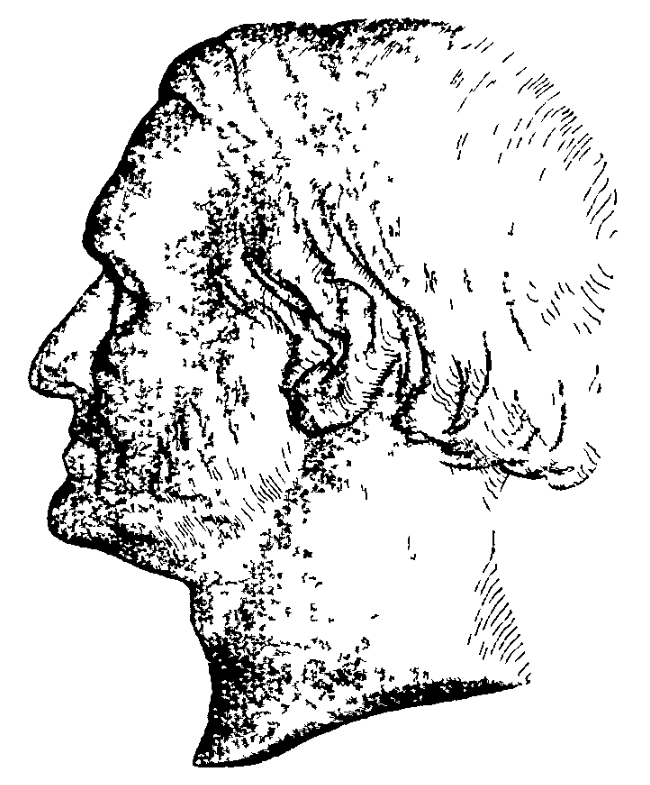
\includegraphics[width=1.6in]{portrait006.png}\par
\medskip
HERAUSGEGEBEN\par
\smallskip
VON DER\par
\smallskip
KÖNIGLICHEN GESELLSCHAFT DER WISSENSCHAFTEN\par
\smallskip
ZU\par
\smallskip
\textls[180]{GÖTTINGEN.}\par
\medskip
IN COMMISSION BEI B. G. TEUBNER IN LEIPZIG.\par
\medskip
1900.
\end{center}
\clearpage

\SourceLeaf{7}% Otherwise blank verso bears a library ownership stamp, outside the historical body.

\SourceLeaf{8}
\thispagestyle{empty}
\vspace*{12em}
\begin{center}
{\Large ARITHMETIK UND ALGEBRA.\par}
\vspace{2em}
NACHTRÄGE ZU BAND I--III.
\end{center}
\clearpage

\SourceLeaf{9}% Blank historical verso, accounted without adding an empty reader page.

\SourceLeaf{10}
\begin{center}
{\Large NACHLASS.\par}
\bigskip
[ZWEI NOTIZEN ÜBER DIE AUFLÖSUNG DER CONGRUENZ
\[
xx+yy+zz\equiv 0\quad(\mathrm{mod.}\ p).]
\]
\end{center}
\begin{center}[1.]\end{center}
\noindent\hspace*{\parindent}Jede Zerlegung einer durch die Primzahl $p$ theilbaren Zahl in vier Quadrate $=aa+bb+cc+dd$ entspricht einer Auflösung der Congruenz
\[
xx+yy+zz\equiv 0\quad(\mathrm{mod.}\ p).
\]
\noindent Zusammen giebt es $pp$ solcher Auflösungen. Die Eine $x\equiv0$, $y\equiv0$, $z\equiv0$ davon weggenommen, zerfallen die übrigen $pp-1$ in $p+1$ Classen, wenn man $x=\xi$, $y=\eta$, $z=\zeta$ mit $x\equiv k\xi$, $y\equiv k\eta$, $z\equiv k\zeta$ zu Einer Classe zählt.

Es sind nämlich proportional
\[
\begin{array}{c|c|c|c}
x & aa+bb & -ad-bc & bd-ac\\
y & ac+bd & ab-cd & aa+dd\\
z & ad-bc & aa+cc & -ab-cd
\end{array}
\]
\begin{center}[2.]\end{center}
\noindent\hspace*{\parindent}Alle Auflösungen der Congruenz
\[
1+xx+yy\equiv0\quad(\mathrm{mod.}\ p)
\]
\noindent zu finden.
\clearpage

\SourceLeaf{11}
Es sind zugleich die Auflösungen der Congruenz
\[
1+(x+iy)^{p+1}\equiv0\quad\text{für}\quad p\equiv3\quad(\mathrm{mod.}\ 4).
\]
\par\indent Aus einem Werthe $x+iy$ folgen alle, indem man für $u$ alle Werthe\\
$0,1,2,3,\, .\, .\, .,p-1$ substituirt, vermöge der Formel\HistoricalNote{[*)]}{[*)}{Neben dieser Entwickelung stehen im Manuscript die Formeln:]
\[
1-xx\equiv yy,\qquad x=1-uy,\qquad 2u-uuy=y
\]
\[
\frac{1-uu}{1+uu}=x,\qquad\frac{2u}{1+uu}=y,
\]
\noindent [welche die Rolle des Zusatzfactors $\dfrac{uu-1+2iu}{uu+1}$ erläutern.]}
\[
(x+iy)\left(\frac{uu-1+2iu}{uu+1}\right)\quad\text{oder}\quad\frac{(x+iy)(u+i)}{u-i}.
\]
\par\indent Für $p\equiv1\ (\mathrm{mod.}\ 4)=aa+bb$ enthält die Formel $\dfrac{b}{a}.\dfrac{u+i}{u-i}$ alle Werthe von $x+iy$, wo nur für $u$ die Werthe $\dfrac{a}{b}$ und $\dfrac{b}{a}$ auszuschliessen sind.

\clearpage\SourceLeaf{12}
\begin{center}\bfseries [NOTIZEN ÜBER CUBISCHE UND BIQUADRATISCHE RESTE.]\end{center}
\begin{center}[1.]\par\smallskip Observatio venustissima inductione facta.\end{center}
\noindent\hspace*{\parindent}2 est Residuum vel non residuum cubicum numeri primi $p$ formae $3n+1$, prout $p$ repraesentabilis est per formam
\[xx+27yy\qquad\text{vel}\qquad4xx+2xy+7yy.\]
\par\noindent\hspace*{\parindent}3 est Residuum vel non residuum, prout $p$ repraesentabilis est per
\[\begin{aligned} &xx+243yy\quad\text{aut}\quad4xx+2xy+61yy\\
\text{vel}\quad&7xx+6xy+36yy\quad\text{aut}\quad9xx+6xy+28yy.\end{aligned}\]
\par\noindent\hspace*{\parindent}5 est $\left.\begin{array}{l}\text{Residuum}\\\text{Nonresiduum}\end{array}\right\}$ si $p$ repraesentatur
\begingroup\small
\[\text{per }\left\{\begin{array}{l}(1,0,675),\ (25,0,27),\ (13,1,52),\ (4,1,169)\\
(7,2,97),\ (9,3,76),\ (19,3,36),\ (25,5,28),\ (25,10,31),\ (27,9,28).\end{array}\right.\]
\endgroup
\begin{center}[2.]\end{center}
\noindent\hspace*{\parindent}Criterium, per quod diiudicatur, utrum numerus $m$ sit residuum cubicum numeri primi $p$ formae $3n+1$.

Fiat
\[4p=aa+27bb\]

\noindent\unskip\SourceLeaf{13}Tunc erit
\begin{center}\footnotesize\setlength{\tabcolsep}{3pt}
\begin{tabular}{@{}rlll@{}}
& &$m\ R\ p$&$m\ N\ p$\\
1)&$m=2$, si&$b$ par&$b$ impar\\
2)&$m=3$&$b$ divis. per 3&\\
3)&\multicolumn{3}{l}{$m={}$ primus alius, si $\dfrac{a+b\sqrt{-27}}{a-b\sqrt{-27}}$ Res. cub. ipsius $m$}\\[5pt]
4)&\multicolumn{3}{l}{$m=6$, si aut $2b$ aut $a+b$ aut $a-b$ per 12 divis.}\\
5)&\multicolumn{3}{l}{$m=10$, si aut $2b$ aut $2a$ aut $a\pm3b$ aut $a\pm9b$ per 20 divis.}\\
6)&$m=12$&\multicolumn{2}{l}{$2b,\qquad a+5b,\qquad a-5b$ per 12}\\
7)&$m=15$&\multicolumn{2}{l}{$b,\qquad 3a+5b,\qquad a\pm b,\qquad a\pm2b$ per 15}\\
8)&$m=20$&\multicolumn{2}{l}{$2b,\qquad2a,\qquad a\pm b,\qquad a\pm7b$ per 20}\\
9)&$m=45$&\multicolumn{2}{l}{$b,\qquad3a+5b,\qquad a\pm4b,\qquad a\pm7b$ per 15}\\
10)&$m=14$&\multicolumn{2}{l}{$2b,\qquad2a,\qquad a\pm5b,\qquad a\pm11b$ per 28}\\
11)&$m=28$&\multicolumn{2}{l}{$2b,\qquad2a,\qquad a\pm3b,\qquad a\pm9b$ per 28.}
\end{tabular}\end{center}
\medskip
\par\noindent\hspace*{\parindent}Criterium, per quod diiudicari potest, utrum numerus $m$ sit residuum biquadraticum numeri primi $p$ formae $4n+1$.

Fiat
\[p=aa+4bb\]
\Needspace{17\baselineskip}
\noindent Tunc erit $m\ R\ p$, si
\begin{center}\small\setlength{\tabcolsep}{3pt}\begin{tabular}{@{}rlll@{}}
1)&$m=-1$ si&$b$ par&$\pm4$ si $b$ par\\
2)&$m=\pm2$ si&$b$ per 4 divisib.&$-4$ generaliter\\
3)&$m=+3$ si&$b$ aut $a+3b$ per 6&\\
4)&$m=-3$ si&$b$ per 3&\\
5)&$m=+5$ si&$b$ per 5&\\
6)&$m=-5$ si&$b$ aut $a+5b$ per 10&\\
7)&$m=+6$&\multicolumn{2}{l}{$b,\qquad2a+3b,\qquad a\pm b$ per 12}\\
8)&$m=-6$&\multicolumn{2}{l}{$b,\qquad2a+3b,\qquad a\pm5b$ per 12}\\
9)&$m=+7$&\multicolumn{2}{l}{$2a+7b,\qquad b,\qquad a\pm5b$ per 14}
\end{tabular}\end{center}

\SourceLeaf{14}
\begin{center}\small\setlength{\tabcolsep}{3pt}\begin{tabular}{@{}rll@{}}
10)&$m=-7$&$a,\qquad b$ per 7\\
11)&$m=+10$ si&$2a+5b,\qquad b,\qquad a\pm7b$ per 20\\
12)&$m=-10$&$2a+5b,\qquad b,\qquad a\pm3b$ per 20\\
13)&$m=+11$&$2a+11b,\qquad b,\qquad2a\pm3b,\qquad a\pm b$ per 22\\
14)&$m=-11$&$b,\qquad a\pm4b$ per 11.
\end{tabular}\end{center}
\begin{center}[3.]\par\smallskip Die cubischen Reste.\end{center}
\noindent\hspace*{\parindent}$p$ eine Primzahl der Form $3m+1$
\[4p=aa+27bb,\]
\par\noindent\hspace*{\parindent}$q$ eine andere Primzahl der Form $3n\pm1$
\[(a+3b\sqrt{-3})^{\frac{q\mp1}{3}}\equiv A\pm B\sqrt{-3}.\]
\par\noindent\hspace*{\parindent}Nun gibt es drei Fälle
\[\begin{array}{rlll}
\text{I.}&B\equiv0\quad\;(\mathrm{mod.}\ q).&\text{Dann ist }q^{\frac{p-1}{3}}\equiv1&\;(\mathrm{mod.}\ p).\\[5pt]
\text{II.}&B\equiv A\quad\;(\mathrm{mod.}\ q).&\text{Dann ist }q^{\frac{p-1}{3}}\equiv-\tfrac12-\tfrac12\dfrac{a}{3b}&\;(\mathrm{mod.}\ p).\\[5pt]
\text{III.}&B\equiv-A\quad\;(\mathrm{mod.}\ q).&\text{Dann ist }q^{\frac{p-1}{3}}\equiv-\tfrac12+\tfrac12\dfrac{a}{3b}&\;(\mathrm{mod.}\ p).
\end{array}\]
\Needspace{9\baselineskip}
\noindent\hspace*{\parindent}Erstes Beispiel.\qquad $\begin{array}[t]{ll}p=13,&q=5\\a=5,&b=1\end{array}$
\[(5+3\sqrt{-3})^2=-2+30\sqrt{-3},\quad B\equiv0\ \mathrm{mod.}\ 5\ \text{also Casus I}\]
\[5^4=625\equiv1.\]
\Needspace{9\baselineskip}
\noindent\hspace*{\parindent}Zweites Beispiel.\qquad $\begin{array}[t]{ll}p=19,&q=5\\a=7,&b=1\end{array}$
\[(7+3\sqrt{-3})^2=22+42\sqrt{-3},\quad B\equiv-A\ \text{also Casus III}\]
\[5^6\equiv7\quad\mathrm{mod.}\ 19,\qquad42\equiv-3+7\quad\mathrm{mod.}\ 19.\]

\Needspace{9\baselineskip}
\noindent\SourceLeaf{15}\hspace*{\parindent}Drittes Beispiel.\qquad $\begin{array}[t]{ll}p=7,&q=5\\a=1,&b=1\end{array}$
\[(1+3\sqrt{-3})^2=-26+6\sqrt{-3},\quad B\equiv+A\quad\mathrm{mod.}\ 5\quad\text{Casus II}\]
\[5^2\equiv4,\qquad24\equiv-3-1\quad\mathrm{mod.}\ 7.\]
\Needspace{9\baselineskip}
\noindent\hspace*{\parindent}Viertes Beispiel.\qquad $p=13,\qquad q=11$
\[(5+3\sqrt{-3})^4=-2696-120\sqrt{-3},\quad A\equiv-1,\quad B=120\equiv-1\]
\[11^4\equiv3,\qquad18+3\equiv-5\quad\mathrm{mod.}\ 13\quad\text{Casus II.}\]
\begin{center}Die biquadratischen Reste.\end{center}
\noindent\hspace*{\parindent}$p$ eine Primzahl von der Form $4n+1$
\[p=aa+4bb,\]
\par\noindent\hspace*{\parindent}$q$ eine Primzahl der Form $4n\pm1$
\[(a+2b\sqrt{-1})^{\frac{q\mp1}{4}}=A\pm B\sqrt{-1}.\]
\par\noindent\hspace*{\parindent}Nun gibt es vier Fälle
\[\begin{array}{rll}
\text{I.}&B\equiv0\ (\mathrm{mod.}\ q),&(\pm q)^{\frac{p-1}{4}}\equiv1\ (\mathrm{mod.}\ p).\\[4pt]
\text{II.}&A\equiv0&(\pm q)^{\frac{p-1}{4}}\equiv-1.\\[4pt]
\text{III.}&A\equiv B&(\pm q)^{\frac{p-1}{4}}\equiv-\dfrac{a}{2b}.\\[8pt]
\text{IV.}&A\equiv-B&(\pm q)^{\frac{p-1}{4}}\equiv\dfrac{a}{2b}.
\end{array}\]
\Needspace{9\baselineskip}
\noindent\hspace*{\parindent}Erstes Beispiel.\qquad $\begin{array}[t]{ll}p=13,&q=5\\a=3,&b=1\end{array}$
\[(3+2\sqrt{-1})^1=3+2\sqrt{-1},\quad A\equiv-B\quad\text{Casus IV}\]
\[5^3\equiv8\equiv\dfrac{3}{2.b}.\]
\Needspace{9\baselineskip}
\noindent\hspace*{\parindent}Zweites Beispiel.\qquad $p=13,\qquad q=7$
\[(3+2\sqrt{-1})^2=5+12\sqrt{-1},\quad A\equiv-B\quad\text{Casus IV}\]
\[(-7)^3\equiv8\equiv\dfrac{3}{2.b}.\]

\Needspace{9\baselineskip}
\noindent\SourceLeaf{16}\hspace*{\parindent}Drittes Beispiel.\qquad $p=13,\qquad q=11$
\[(3+2\sqrt{-1})^3=-9+46\sqrt{-1},\quad A\equiv-B\quad\text{Casus IV}\]
\[(-11)^3\equiv8\equiv\dfrac{3}{2.b}.\]
\Needspace{9\baselineskip}
\noindent\hspace*{\parindent}Viertes Beispiel.\qquad $p=17,\qquad q=11$
\[(1+4\sqrt{-1})^3=-47-52\sqrt{-1},\quad-47=A,\quad+52=B\]
\[A\equiv B\quad\text{Casus III}\]
\[(-11)^4\equiv4\equiv-\tfrac14.\]
\begin{center}[4.]\end{center}
\noindent\hspace*{\parindent}Es sei $p$ eine Primzahl, $n$ eine Primzahl $=3m+1$, $R$ Wurzel der Gleichung $x^3-1=0$, $r$ Wurzel der Gleichung $r^n-1=0$, $g$ Radix primitiva für mod. $n$.
\[r+Rr^g+R^2r^{g^2}+R^3r^{g^3}+\ldots+R^{n-2}r^{g^{n-2}}=P,\]
\[P^3=\tfrac12 n(M+N\sqrt{-27}),\]
\noindent wo
\[M\equiv1\ (\mathrm{mod.}\ 3),\qquad0\equiv M+3N(g^m-g^{2m})\ (\mathrm{mod.}\ n)\]
\[3k=M+2\]
\[a=\tfrac19(n+1+M)\]
\[b-c=N.\]
\[P^{pp}\equiv r^{pp}+Rr^{ppg}+\ldots\equiv P(R^{\mathrm{ind.}\,p})\]
\begingroup\footnotesize
\[\begin{array}{r@{}l|c}
&1&0\\[3pt]
\{\tfrac12 n(M+N\sqrt{-27})\}^{\frac13(pp-1)}\equiv{}&-\tfrac12+\tfrac12\sqrt{-3}\ (\mathrm{mod.}\ p)&\mathrm{ind.}\ p\equiv1\ (\mathrm{mod.}\ 3)\\[3pt]
&-\tfrac12-\tfrac12\sqrt{-3}&2
\end{array}\]
\endgroup
\[4n=(M+N\sqrt{-27})(M-N\sqrt{-27})\]
\[\dfrac{M}{3N}\equiv g^{2m}-g^m,\qquad-1\equiv g^{2m}+g^m\]
\begingroup\footnotesize
\[\begin{array}{r@{}l|c}
&1&1\\[3pt]
\left\{\dfrac{M-N\sqrt{-27}}{M+N\sqrt{-27}}\right\}^{\frac13(pp-1)}\equiv{}&-\tfrac12+\tfrac12\sqrt{-3}\ (\mathrm{mod.}\ p)&p^{\frac13(n-1)}\equiv-\tfrac12-\tfrac12\dfrac{M}{3N}\ (\mathrm{mod.}\ n)\\[5pt]
&-\tfrac12-\tfrac12\sqrt{-3}&-\tfrac12+\tfrac12\dfrac{M}{3N}
\end{array}\]
\endgroup

\SourceLeaf{17}
\[P^4\equiv PR^{\mathrm{ind.}\,2}\]
\[\tfrac12 M+\tfrac32 N(R-R^2)=\tfrac12(M+3N)+3NR\]
\[\begin{array}{r@{}l|cc}
&1&\tfrac12(M+3N)\ \text{impar}&3N\ \text{par}\\[4pt]
2^{\frac13(n-1)}\equiv{}&-\tfrac12+\tfrac12\dfrac{M}{3N}\ (\mathrm{mod.}\ n)&\text{impar}&\text{impar}\\[5pt]
&-\tfrac12-\tfrac12\dfrac{M}{3N}&\text{par}&\text{impar.}
\end{array}\]
\begin{center}Für den cubischen Rest 3.\end{center}
\[\begin{aligned}
p^3&=m(a-1)+\{m+(a-1)^2+bb+cc\}p\\
&\qquad+\{(a-1)b+bc+ac\}p'\\
&\qquad+\{(a-1)c+ab+bc\}p''\\
&=A+Bp+Cp'+Dp''.
\end{aligned}\]
\noindent Nun ist
\[\begin{array}{rl}1)&aa+bb+cc=ab+ac+bc+a\\2)&a+b+c=m\\3)&3k-2=M\\4)&4a=kk+3NN\\5)&4n=(3k-2)^2+27NN\\6)&4m=3kk-4k+9NN.\end{array}\]
\noindent Hieraus folgt
\[\begin{aligned}A&\equiv0\quad\;(\mathrm{mod.}\ 3)\\ B&=\tfrac13(mm-a)-a+m+1\\ C&=\tfrac13(mm-a)-b\\D&=\tfrac13(mm-a)-c\end{aligned}\]
\[\begin{aligned}\tfrac43(mm-a)&\equiv-2k^3+kk-NN\quad\;(\mathrm{mod.}\ 3)\\
&\equiv kk+k-NN\quad\;(\mathrm{mod.}\ 3)\\
&\equiv4a-4m-NN\quad\;(\mathrm{mod.}\ 3).\end{aligned}\]

\noindent\unskip\SourceLeaf{18}Also
\[\begin{aligned}B&\equiv-NN+1\equiv-(b-c)^2+1\\C&\equiv-NN+b-c\equiv-(b-c)^2+b-c\\D&\equiv-NN-(b-c)\equiv-(b-c)^2-(b-c)\end{aligned}\]
\[\begin{array}{rrrr}
b-c\equiv0&B\equiv1&C\equiv0&D\equiv0\\1&0&0&1\\2&0&1&0.
\end{array}\]
\par\noindent\hspace*{\parindent}Ist also 3 Res. $n$, so ist $N$ durch 3 theilbar.
\Needspace{10\baselineskip}
\begingroup\small
\begin{center}BEMERKUNGEN ZU DEN VORSTEHENDEN NOTIZEN ÜBER CUBISCHE UND BIQUADRATISCHE RESTE.\end{center}
\noindent\hspace*{\parindent}Die Notiz [1] ist von \textsc{Gauss} auf das Vorsatzblatt des Einbandes seines Handexemplars der Disquisitiones arithmeticae geschrieben. Die Angaben unter [2] finden sich in einem mit der Überschrift »Uraniae sacrum« versehenen Hefte, und ebenda folgen zwei Seiten später die beiden allgemeinen Sätze [3]. Die Entwicklungen unter [4] sind einigen losen Zetteln entnommen.

\textsc{Gauss} giebt zu Beginn seiner Commentatio prima über die Theorie der biquadratischen Reste an, dass er mit dem Jahre 1805 begonnen habe, die Theorie der cubischen und biquadratischen Reste zu durchforschen. Die hier unter [2] und [3] gegebenen Entwicklungen folgen in dem genannten Hefte unmittelbar auf Notizen, welche das Datum 1804 tragen. Die »Observatio venustissima« [1], welche weniger weit greifend ist, als die »Criterien« [2] und [3], kann zeitlich nicht wohl später liegen als letztere. Man wird es demnach hier mit den ältesten \textsc{Gauss}'schen Untersuchungen und damit überhaupt mit den ältesten Urkunden über die höheren Reciprocitätsgesetze zu thun haben.

Wie die Observatio so sind vermuthlich auch die Criterien Inductionsresultate. Es ist aber sehr bemerkenswerth, dass schon hier bei den Criterien die Zerlegung der quadratischen Form $aa+27bb$ in ihre beiden complexen Factoren und damit der Zahl $p$ in ihre beiden complexen Primtheiler auftritt. Es war bereits hiermit die Bahn gewonnen, auf welcher \textsc{Gauss} späterhin wenigstens das biquadratische Reciprocitätsgesetz in seine einfachste Gestalt kleidete. Bei gewissen Beweisansätzen des allgemeinen cubischen Reciprocitätssatzes (siehe die gleich folgenden Notizen), welche jedenfalls vor 1809 liegen, ist übrigens \textsc{Gauss} wenigstens am Beginn allein vom Gebrauch rationaler Zahlen ausgegangen.

Die zu Anfang von [2] unter 3) gemachte Angabe lässt sich als Specialfall aus dem ersten allgemeinen Satze unter [3] entnehmen. Letzterer liefert direct den Reciprocitätssatz in der allgemeinsten und einfachsten Gestalt, falls $p=3m+1$ und $q=3n-1$ ist. Der cubische Charakter des Primtheiler $\pi_1=\dfrac{a+3b\sqrt{-3}}{2}$ in Bezug auf $q$ ist nämlich durch
\[\left[\frac{\pi_1}{q}\right]\equiv(A-B\sqrt{-3})^{q-1}\quad\;(\mathrm{mod.}\ q)\]

\noindent\unskip\SourceLeaf{19}angegeben, ein Ausdruck, der entweder mit 1, $\rho$ oder $\rho^2$ mod. $q$ congruent ist, unter $\rho$ die Einheitswurzel
$\dfrac{-1+i\sqrt{3}}{2}$ verstanden. Da nun im Gebiete der aus $\rho$ zu bildenden ganzen complexen Zahlen die Lösungen
der Congruenz $x^{q-1}\equiv 1\;(\mathrm{mod.}\ q)$ die $(q-1)$ von 0 verschiedenen rationalen ganzen Reste mod. $q$ sind,
so kommt die von \textsc{Gauss} vermöge der Congruenzen $B\equiv 0$, $B\equiv A$, $B\equiv -A\;(\mathrm{mod.}\ q)$ vollzogene Dreitheilung darauf hinaus, dass der cubische Charakter $\left[\dfrac{\pi_1}{q}\right]$ gleich 1 bez. $\rho$, $\rho^2$ ist. Im anderen Falle $q=3n+1$
ist hier der einfachste Ausdruck des Reciprocitätssatzes deshalb noch nicht erreicht, weil die Zerlegung von
$q$ in seine Primtheiler noch nicht vollzogen ist. Die Beziehung des \textsc{Gauss}'schen Theorems zum Reciprocitätsgesetze ist die folgende:

Sind die Zerlegungen der rationalen Primzahlen $p, q$ in ihre primären Primfactoren gegeben durch:
\[ p=\pi_1.\pi_2,\qquad q=\varkappa_1.\varkappa_2,\qquad \pi_k'=2\pi_k=a\pm 3b\sqrt{-3}, \]
so hat man zu setzen:
\[
\left.\begin{array}{l}
\left[\dfrac{\pi_1'}{\varkappa_1}\right]=\rho^{\varepsilon_1}\equiv {\pi_1'}^{\frac{q-1}{3}}\equiv A+B\rho-B\rho^2 \\[2mm]
\left[\dfrac{\pi_2'}{\varkappa_1}\right]=\rho^{\varepsilon_2}\equiv {\pi_2'}^{\frac{q-1}{3}}\equiv A-B\rho+B\rho^2
\end{array}\right\}(\mathrm{mod.}\ \varkappa_1).
\]

\noindent Die \textsc{Gauss}'sche Dreitheilung kommt dann mit der folgenden überein:
\[
\text{I.}\quad \varepsilon_1\equiv \varepsilon_2 (\mathrm{mod.}\ 3),\qquad \left[\dfrac{\pi_1'}{\varkappa_1}\right]=\left[\dfrac{\pi_2'}{\varkappa_1}\right],
\]
\[
\text{II.}\quad \varepsilon_1\equiv \varepsilon_2+1\;(\mathrm{mod.}\ 3),\qquad \left[\dfrac{\pi_1'}{\varkappa_1}\right]=\rho\left[\dfrac{\pi_2'}{\varkappa_1}\right],
\]
\[
\text{III.}\quad \varepsilon_1\equiv \varepsilon_2-1\;(\mathrm{mod.}\ 3),\qquad \left[\dfrac{\pi_1'}{\varkappa_1}\right]=\rho^2\left[\dfrac{\pi_2'}{\varkappa_1}\right],
\]
wobei in den drei letzten Gleichungen offenbar auch $\pi_k$ an Stelle von $\pi_k'$ treten kann. Liegt nämlich z.\,B.
der Fall II vor, so folgt durch Addition und Subtraction obiger Congruenzen in Bezug auf den Modul $\varkappa_1$:
\[
2A\equiv \rho^{\varepsilon_2}(1+\rho)\equiv -\rho^{\varepsilon_2-1},\qquad 2B\equiv -\rho^{\varepsilon_2-1}\qquad\;(\mathrm{mod.}\ \varkappa_1),
\]
so dass $(A-B)$ durch $\varkappa_1$ und als rationale Zahl demnach auch durch $q$ theilbar ist. Man hat also wirklich $B\equiv A\;(\mathrm{mod.}\ q)$. Das Reciprocitätsgesetz liefert nun:
\[
\left[\dfrac{\pi_1'}{\varkappa_1}\right]=\left[\dfrac{2}{\varkappa_1}\right].\left[\dfrac{\pi_1}{\varkappa_1}\right]=\left[\dfrac{2}{\varkappa_1}\right].\left[\dfrac{\varkappa_1}{\pi_1}\right],
\]
\[
\left[\dfrac{\pi_2'}{\varkappa_1}\right]=\left[\dfrac{2}{\varkappa_1}\right].\left[\dfrac{\pi_2}{\varkappa_1}\right]=\left[\dfrac{2}{\varkappa_1}\right].\left[\dfrac{\varkappa_1}{\pi_2}\right],
\]
so dass man für den Fall II weiter gewinnt:
\[
\left[\dfrac{\varkappa_1}{\pi_1}\right]=\rho\left[\dfrac{\varkappa_1}{\pi_2}\right]=\rho\left[\dfrac{\varkappa_2}{\pi_1}\right]^2,\qquad
\left[\dfrac{\varkappa_1}{\pi_1}\right].\left[\dfrac{\varkappa_2}{\pi_1}\right]=\left[\dfrac{q}{\pi_1}\right]=\rho,
\]
\[
\left[\dfrac{q}{\pi_1}\right]\equiv q^{\frac{p-1}{3}}\equiv -\tfrac12+\tfrac12\sqrt{-3}\equiv -\tfrac12-\tfrac12\dfrac{a}{3b}\qquad\;(\mathrm{mod.}\ \pi_1).
\]
Soll aber die rationale Zahl $q^{\frac{p-1}{3}}+\tfrac12+\tfrac12\dfrac{a}{3b}\equiv 0 \mathrm{mod.}\ \pi_1$ sein, so ist sie auch durch $\pi_2$ und also durch $p$
theilbar. Hiermit ist die unter II von \textsc{Gauss} angegebene Congruenz in Bezug auf den Modul $p$ gewonnen.
Ebenso erledigen sich die Fälle I und III.

\SourceLeaf{20}

Die Umkehrung der vorstehenden Entwicklung lehrt, dass man aus den \textsc{Gauss}'schen Angaben im
Falle $q=3n+1$ zunächst auf die Proportion:
\[
\left[\dfrac{\varkappa_1}{\pi_1}\right]:\left[\dfrac{\pi_1}{\varkappa_1}\right]=\left[\dfrac{\varkappa_1}{\pi_2}\right]:\left[\dfrac{\pi_2}{\varkappa_1}\right]
\]
schliessen kann. Unter nochmaliger Benutzung des in dieser Proportion ausgesprochenen Gesetzes findet man:
\[
\dfrac{\left[\dfrac{\varkappa_1}{\pi_1}\right]}{\left[\dfrac{\pi_1}{\varkappa_1}\right]}=\dfrac{\left[\dfrac{\varkappa_2}{\pi_1}\right]}{\left[\dfrac{\pi_1}{\varkappa_2}\right]}=\dfrac{\left[\dfrac{\varkappa_1}{\pi_2}\right]^2}{\left[\dfrac{\pi_2}{\varkappa_1}\right]^2}
\quad\text{und also}\quad
\dfrac{\left[\dfrac{\varkappa_1}{\pi_2}\right]}{\left[\dfrac{\pi_2}{\varkappa_1}\right]}=\dfrac{\left[\dfrac{\varkappa_1}{\pi_2}\right]^3}{\left[\dfrac{\pi_2}{\varkappa_1}\right]^2}.
\]
Da hieraus $\left[\dfrac{\varkappa_1}{\pi_2}\right]=\left[\dfrac{\pi_2}{\varkappa_1}\right]$ hervorgeht, so ist auch für $q=3n+1$ in \textsc{Gauss}' Angaben das allgemeine Reciprocitätsgesetz in seiner einfachsten Form implicite enthalten.

Unter [4] sind diejenigen Aufzeichnungen gesammelt, durch welche \textsc{Gauss} seine cubischen Reciprocitätstheoreme bewiesen hat. Da diese Aufzeichnungen mehreren losen Zetteln ohne Datumangabe entnommen sind, so lässt sich die Entstehungszeit der fraglichen Beweise nicht mit Sicherheit angeben. Es ist
aber wahrscheinlich, dass die Entwicklungen alsbald nach Gewinnung der »Observatio« und der »Criterien«
durchgeführt sind; sie schliessen sich nämlich im Gedankengang sehr eng an die ersten Angaben unter [2]
und übrigens an den Art. 358 der Disquisitiones arithmeticae an, und andererseits ist \textsc{Gauss} zufolge seiner
eigenen Aussage\HistoricalNote{\textsuperscript{*)}}{*)}{Siehe den Art. 33 der am 24. August 1808 der Göttinger Societät vorgelegten Abhandlung »Summatio quarumdam serierum singularium«.} jedenfalls vor Mitte des Jahres 1808 im Besitze des sechsten Beweises des quadratischen
Reciprocitätsgesetzes gewesen, welcher mit den hier gemeinten Beweisen am nächsten verwandt ist.

Dem \textsc{Gauss}'schen Beweise des cubischen Reciprocitätssatzes liegt die Kreistheilung zu Grunde. Die
einzelnen Formeln unter [4] können entweder unmittelbar aus Art. 358 der Disquisitiones arithmeticae entnommen werden, oder sie lassen sich doch mit sehr geringer Mühe aus den dortigen Entwicklungen ableiten.
Die Congruenz:
\[
P^{pp}\equiv r^{pp}+Rr^{ppg}+\ldots\equiv P(R^{\mathrm{ind.}\,p})
\]
bezieht sich auf den Modul $p$ und entspringt aus dem Umstande, dass alle von 1 verschiedenen Polynomialcoefficienten der Potenz $pp$ durch $p$ theilbar sind. Die Fallunterscheidung
\[
\left\{\dfrac{M-N\sqrt{-27}}{M+N\sqrt{-27}}\right\}^{\frac13(pp-1)}\equiv 1,\quad -\tfrac12+\tfrac12\sqrt{-3},\quad -\tfrac12-\tfrac12\sqrt{-3}\qquad\;(\mathrm{mod.}\ p)
\]
correspondirt sowohl für $p=3m-1$ wie $p=3m+1$ genau der oben unter I, II und III getroffenen
Unterscheidung $B\equiv 0\;(\mathrm{mod.}\ q)$, etc. Die Zuordnung jener drei Congruenzen zu den folgenden
\[
p^{\frac13(n-1)}\equiv 1,\quad -\tfrac12-\tfrac12\dfrac{M}{3N},\quad -\tfrac12+\tfrac12\dfrac{M}{3N}\qquad\;(\mathrm{mod.}\ n),
\]
wie sie in [4] entwickelt wird, enthält demnach bereits einen vollständigen Beweis der \textsc{Gauss}'schen Angaben
und damit implicite des allgemeinen cubischen Reciprocitätssatzes.

Die weiteren Ausführungen unter [4] betreffen die Criterien über die cubischen Reste 2 und 3.
Wegen des cubischen Restes 3 bemerke man nur, dass (unter Benutzung der in [4] gebrauchten Bezeichnung)
$p^3\equiv p, p'$ oder $p''\;(\mathrm{mod.}\ 3)$ zutrifft, je nachdem ind.\,$3\equiv 0, 1$ oder $2\;(\mathrm{mod.}\ 3)$ stattfindet. Die Bedingung
$N\equiv 0\;(\mathrm{mod.}\ 3)$, damit 3 cubischer Rest von $n$ ist, ergiebt sich daraufhin unmittelbar aus den Schlussangaben von [4].


\SourceLeaf{21}

Die Observatio kann aus den Criterien leicht abgeleitet werden. Z.\,B. war für den cubischen Rest 3
soeben die Bedingung $N\equiv 0\;(\mathrm{mod.}\ 3)$ gewonnen und unter [2] ebenso angegeben. Sind nun $M$ und $N$
gerade, so setze man:
\[ M=2x,\qquad N=6y, \]
so dass aus $4n=M^2+27N^2$ die Darstellbarkeit von $n$ in der quadratischen Form der Determinante $-243$:
\[ n=x^2+243y^2 \]
vermöge ganzzahliger $x, y$ entspringt. Umgekehrt folgt bei der Möglichkeit einer solchen Darstellung von $n$
die Gültigkeit der Congruenz $N\equiv 0\;(\mathrm{mod.}\ 3)$. Sind $M$ und $N$ ungerade, so setze man unter richtiger Auswahl des Vorzeichens:
\[ M\pm\dfrac{N}{3}=4x,\qquad \mp\dfrac{N}{3}=y, \]
woraus man die Darstellung gewinnt:
\[ n=4x^2+2xy+61y^2. \]
Aus dieser Formel würde umgekehrt folgen $N\equiv 0\;(\mathrm{mod.}\ 3)$, so dass 3 stets und nur dann cubischer Rest
von $n$ ist, wenn $n$ durch eine der Formen $(1,0,243)$, $(4,1,61)$, darstellbar ist.

Durch Herrn R. \textsc{Dedekind}, dem ich mehrere für mich sehr förderliche Unterhaltungen über die in
Rede stehenden Gegenstände verdanke, bin ich darauf aufmerksam gemacht, dass für den Fall des cubischen
Nichtrestes 3 von $n$ \textsc{Gauss}' Angaben nicht ganz vollständig sind. Es giebt insgesammt neun Classen ursprünglicher Formen erster Art der Determinante $D=-243$, deren reducirte Formen die folgenden sind:
\[ (1,0,243),\quad (4,\pm1,61),\quad (13,\pm2,19),\quad (7,\pm3,36),\quad (9,\pm3,28). \]
Es fehlen in [1] die Formen $(13,\pm2,19)$. Das Theorem muss demnach so lauten, dass 3 stets und nur
dann cubischer Nichtrest von $n$ ist, wenn $n$ eine Darstellung in einer der Formen gestattet:
\[ n=13xx+4xy+19yy, \]
\[ n=7xx+6xy+36yy, \]
\[ n=9xx+6xy+28yy. \]
Diese Darstellungen erreicht man immer unter richtiger Fixirung des Vorzeichens durch folgende Transformationen:
\[ \text{I. Wenn } M\equiv N\equiv 1\;(\mathrm{mod.}\ 2),\quad M\pm 7N\equiv 0\;(\mathrm{mod.}\ 12), \]
\[ M=5x+7y,\qquad \pm N=x-y. \]
\[ \text{II. Wenn } M\equiv N\equiv 1\;(\mathrm{mod.}\ 2),\quad M\pm 7N\equiv 6\;(\mathrm{mod.}\ 12), \]
\[ M=x+6y,\qquad \mp N=x. \]
\[ \text{III. Wenn } M\equiv N\equiv 0\;(\mathrm{mod.}\ 2),\quad M\pm N\equiv 0\;(\mathrm{mod.}\ 3), \]
\[ M=6x+2y,\qquad \mp N=2y. \]
\par\noindent\hspace*{\parindent}Die über die Zahl 5 unter 1 gemachten Angaben folgen in ähnlicher Weise aus dem Restcriterium
$MN\equiv 0\;(\mathrm{mod.}\ 5)$.

Übrigens sei noch bemerkt, dass sich im Original der Notiz [1] eine bis 223 fortgesetzte Tabelle derjenigen Primzahlen $p=3n+1$ findet, von denen die Zahlen 2, 3, 5, 7 cubische Reste sind.

\hfill \textsc{Fricke.}

\endgroup

\clearpage\SourceLeaf{22}
\begin{center}
\bfseries ZUR THEORIE DER CUBISCHEN RESTE.
\end{center}



\begin{center}
[1.]
\end{center}

\[ p=mm+3nn \text{ eine Primzahl.} \]

\noindent\hspace*{\parindent}Man setze für irgend eine ganze durch $p$ nicht theilbare Zahl $x$
\[
\left[\dfrac{2mx}{p}\right]=\alpha,\qquad \left[\dfrac{(3n-m)x}{p}\right]=\beta,\qquad \left[\dfrac{(-3n-m)x}{p}\right]=\gamma.
\]
\noindent Hieraus wird, wie man leicht sieht,
\[
\dfrac{2mx}{p}-\alpha+\dfrac{(3n-m)x}{p}-\beta+\dfrac{(-3n-m)x}{p}-\gamma
\]
die Summe aus drei echten Brüchen, und muss daher exclusive zwischen den
Grenzen 0 und 3 liegen; da aber offenbar dieselbe Summe $=-\alpha-\beta-\gamma$, also
eine ganze Zahl ist, so kann sie keinen andern Werth als $+1$ und $+2$ haben.
Es ist also entweder
\[ \alpha+\beta+\gamma=-1\quad\text{oder}\quad \alpha+\beta+\gamma=-2. \]

\noindent Hieraus folgt ferner, dass die Grössen $\alpha, \beta, \gamma$ nicht alle drei unter einander
nach dem Modulus 3 congruent sein können; unter den Differenzen $\alpha-\beta$, $\beta-\gamma$,
$\gamma-\alpha$ wird also wenigstens Eine (und eben deswegen wenigstens noch eine,
%
\SourceLeaf{23}
weil die Summe von allen $=0$) sein, die nicht $\equiv 0$ ist. Ebenso wenig
aber können die Grössen $\alpha, \beta, \gamma$ alle unter einander
incongruent sein, weil sie sonst, gleichviel in welcher Ordnung, den Zahlen
$0, 1, 2$ congruent sein und also ihre Summe durch $3$ theilbar sein
müsste; es wird folglich unter den Differenzen $\alpha-\beta$,
$\beta-\gamma$, $\gamma-\alpha$ gewiss Eine, aber auch nur Eine sein, die
$\equiv 0$ ist. Es gibt mithin drei Fälle, die einander ausschliessen:

\[
\text{I.} \quad \text{Wenn } \beta \equiv \gamma \quad(\mathrm{mod.}\ 3)
\]
\[
\text{II.} \quad \text{Wenn } \gamma \equiv \alpha \quad(\mathrm{mod.}\ 3)
\]
\[
\text{III.} \quad \text{Wenn } \alpha \equiv \beta \quad(\mathrm{mod.}\ 3).
\]

Welcher dieser drei Fälle statthat, hängt von $x$ ab; wir werden daher nach
Maassgabe dieser drei Fälle sämmtliche durch $p$ nicht theilbare Zahlen in
drei Classen theilen, in die erste nämlich diejenigen setzen, wo der
erste; in die zweite die, wo der zweite; in die dritte die, wo der dritte
Fall stattfindet.

\textls[100]{Erstes Theorem:} Alle nach dem Modulus $p$ congruente Zahlen gehören in
Einerlei Classe.

\textls[100]{Zweites Theorem:} Gleiche, aber mit entgegengesetzten Zeichen afficirte
Zahlen gehören in Eine Classe.

Hieraus ist klar, dass man bloss die Zahlen $1, 2, 3, \ldots,
\frac{1}{2}(p-1)$ zu classificiren braucht, um sofort alle übrigen
classificiren zu können.

\textls[100]{Drittes Theorem:} Die Zahlen $(3n-m)x$, $2mx$ gehören in zwei auf einander
folgende Classen.

\textls[100]{Viertes Theorem:} Also wenn $\dfrac{2n-m}{3m} \equiv f$, also

\[
1+f+ff \equiv 0 \quad(\mathrm{mod.}\ p), \qquad 1 \equiv f^3 \quad(\mathrm{mod.}\ p),
\]
\noindent so gehören $x$ und die Reste von $fx$, $ffx$ in drei in umgekehrter
Ordnung auf einander folgende Classen.

%
\clearpage\SourceLeaf{24}
\begin{center}\textls[100]{Beispiele der Abtheilungen.}\end{center}


\begingroup\small
\[p = 7 = 4+3, \qquad 4,\quad 1,\quad -5\]
\begin{center}\begin{tabular}{@{}rl@{}}
I. & 3.\ 4.\\
II. & 2.\ 5.\\
III. & 1.\ 6.\end{tabular}\end{center}
\[p = 13 = 1+12, \qquad 2,\quad 5,\quad -7\]
\begin{center}\begin{tabular}{@{}rl@{}}
I. & 3.\ 6.\ 7.\ 10.\\
II. & 4.\ 5.\ 8.\ 9.\\
III. & 1.\ 2.\ 11.\ 12.\end{tabular}\end{center}
\[p = 19 = 16+3, \qquad 8,\quad -1,\quad -7\]
\begin{center}\begin{tabular}{@{}rl@{}}
I. & 1.\ 2.\ 9.\ 10.\ 17.\ 18.\\
II. & 3.\ 4.\ 8.\ 11.\ 15.\ 16.\\
III. & 5.\ 6.\ 7.\ 12.\ 13.\ 14.\end{tabular}\end{center}
\[p = 31 = 4+27, \qquad 4,\quad 7,\quad -11\]
\begin{center}\begin{tabular}{@{}rl@{}}
I. & 5.\ 9.\ 10.\ 11.\ 15.\ 16.\ 20.\ 21.\ 22.\ 26.\\
II. & 6.\ 7.\ 12.\ 13.\ 14.\ 17.\ 18.\ 19.\ 24.\ 25.\\
III. & 1.\ 2.\ 3.\ 4.\ 8.\ 23.\ 27.\ 28.\ 29.\ 30.\end{tabular}\end{center}
\[p = 37 = 25+12, \qquad 10,\quad 1,\quad -11\]
\begin{center}\begin{tabular}{@{}rl@{}}
I. & 7.\ 8.\ 9,\ 10.\ 17.\ 18.\ 19.\ 20.\ 27.\ 28.\ 29.\ 30.\\
II. & 4.\ 5.\ 6.\ 11.\ 15.\ 16.\ 21.\ 22.\ 26.\ 31.\ 32.\ 33.\\
III. & 1.\ 2.\ 3.\ 12.\ 13.\ 14.\ 23.\ 24.\ 25.\ 34.\ 35.\ 36.\end{tabular}\end{center}
\[p = 43 = 16+27, \qquad 8,\quad 5,\quad -13\]
\begin{center}\begin{tabular}{@{}rl@{}}
I. & 7.\ 8.\ 14.\ 15.\ 16.\ 20.\ 21.\ 22.\ 23.\ 27.\ 28.\ 29.\ 35.\ 36.\\
II. & 6.\ 11.\ 12.\ 13.\ 17.\ 18.\ 19.\ 24.\ 25.\ 26.\ 30.\ 31.\ 32.\ 37.\\
III. & 1.\ 2.\ 3.\ 4.\ 5.\ 9.\ 10.\ 33.\ 34.\ 38.\ 39.\ 40.\ 41.\ 42.\end{tabular}\end{center}
\begin{center}
\begin{tabular}[t]{c|c|c}
\multicolumn{3}{c}{$7,\quad2-\rho$}\\\hline
$1$&$-\rho\rho$&$\rho$\\
$-1$&$\rho\rho$&$-\rho$
\end{tabular}\qquad
\begin{tabular}[t]{c|c|c}
\multicolumn{3}{c}{$13,\quad3-\rho$}\\\hline
$1$&$1-\rho$&$-\rho\rho$\\
$1-\rho\rho$&$\rho$&$\rho-\rho\rho$\\
$-1$&$-1+\rho$&$\rho\rho$\\
$-1+\rho\rho$&$-\rho$&$-\rho+\rho\rho$
\end{tabular}
\end{center}\endgroup
%
\clearpage\SourceLeaf{25}
\begin{center}\begin{tikzpicture}[x=.195pt,y=-.195pt]
\path[use as bounding box] (0,0) rectangle (1750,1100);
\path[fill=black,even odd rule] (414,171) -- (413,174) -- (411,176) -- (411,181) -- (408,185) -- (408,188) -- (406,192) -- (406,197) -- (405,198) -- (405,209) -- (403,212) -- (403,218) -- (401,221) -- (401,224) -- (400,225) -- (399,231) -- (396,235) -- (396,237) -- (394,239) -- (394,241) -- (387,249) -- (386,252) -- (383,255) -- (382,258) -- (379,261) -- (379,262) -- (376,265) -- (375,265) -- (374,267) -- (355,285) -- (355,286) -- (351,290) -- (348,295) -- (344,299) -- (344,302) -- (342,306) -- (340,308) -- (339,308) -- (338,310) -- (338,313) -- (336,315) -- (334,319) -- (333,325) -- (331,327) -- (331,329) -- (330,330) -- (330,334) -- (328,336) -- (326,340) -- (326,343) -- (324,345) -- (322,349) -- (322,351) -- (321,352) -- (321,354) -- (322,355) -- (319,359) -- (319,362) -- (318,363) -- (317,368) -- (311,379) -- (311,382) -- (309,384) -- (309,389) -- (308,390) -- (307,397) -- (305,400) -- (305,403) -- (303,405) -- (302,416) -- (301,417) -- (301,422) -- (299,425) -- (299,429) -- (297,431) -- (297,434) -- (295,437) -- (295,439) -- (292,442) -- (292,445) -- (290,448) -- (290,451) -- (289,452) -- (290,456) -- (289,457) -- (289,464) -- (288,465) -- (289,467) -- (289,469) -- (288,470) -- (288,474) -- (290,478) -- (290,484) -- (291,485) -- (291,491) -- (292,492) -- (291,496) -- (292,497) -- (293,509) -- (294,510) -- (294,513) -- (295,514) -- (295,520) -- (296,521) -- (296,527) -- (297,528) -- (297,532) -- (296,533) -- (296,535) -- (297,536) -- (297,547) -- (298,548) -- (297,551) -- (298,552) -- (298,556) -- (299,557) -- (299,578) -- (301,580) -- (301,582) -- (302,583) -- (302,587) -- (304,590) -- (304,592) -- (307,595) -- (306,599) -- (308,603) -- (308,609) -- (309,610) -- (309,612) -- (311,614) -- (311,618) -- (313,620) -- (314,626) -- (317,631) -- (318,654) -- (319,655) -- (318,678) -- (317,679) -- (317,686) -- (315,689) -- (315,691) -- (311,695) -- (311,698) -- (309,700) -- (309,702) -- (308,703) -- (308,709) -- (307,710) -- (307,713) -- (308,714) -- (307,715) -- (307,719) -- (308,720) -- (308,723) -- (310,726) -- (310,729) -- (314,737) -- (314,739) -- (317,743) -- (316,744) -- (317,754) -- (316,755) -- (316,760) -- (315,761) -- (315,763) -- (316,764) -- (315,765) -- (315,769) -- (313,773) -- (315,777) -- (316,793) -- (322,805) -- (324,807) -- (324,809) -- (326,811) -- (326,817) -- (327,818) -- (327,821) -- (329,823) -- (329,826) -- (331,830) -- (331,844) -- (330,846) -- (332,848) -- (332,852) -- (331,853) -- (331,855) -- (332,856) -- (332,862) -- (335,869) -- (335,873) -- (337,875) -- (339,881) -- (344,886) -- (344,888) -- (352,896) -- (352,897) -- (369,913) -- (370,916) -- (378,926) -- (381,933) -- (387,940) -- (388,943) -- (393,948) -- (396,953) -- (396,955) -- (399,958) -- (400,963) -- (404,967) -- (405,973) -- (407,975) -- (408,980) -- (413,988) -- (430,1003) -- (434,1005) -- (439,1010) -- (443,1011) -- (446,1015) -- (448,1016) -- (451,1016) -- (454,1018) -- (457,1018) -- (458,1019) -- (462,1019) -- (463,1020) -- (472,1021) -- (475,1023) -- (481,1023) -- (482,1024) -- (488,1024) -- (489,1025) -- (491,1025) -- (492,1024) -- (510,1024) -- (511,1023) -- (518,1023) -- (519,1022) -- (522,1022) -- (528,1019) -- (530,1017) -- (532,1017) -- (533,1016) -- (537,1016) -- (538,1015) -- (541,1015) -- (542,1014) -- (546,1014) -- (547,1013) -- (550,1014) -- (551,1013) -- (562,1012) -- (563,1011) -- (577,1011) -- (582,1014) -- (584,1013) -- (589,1013) -- (590,1014) -- (599,1015) -- (601,1017) -- (603,1017) -- (607,1019) -- (610,1019) -- (612,1021) -- (616,1021) -- (618,1023) -- (621,1022) -- (622,1023) -- (626,1023) -- (627,1024) -- (655,1024) -- (656,1023) -- (664,1023) -- (668,1021) -- (680,1021) -- (681,1020) -- (684,1020) -- (685,1019) -- (699,1019) -- (700,1018) -- (705,1018) -- (709,1016) -- (714,1016) -- (717,1014) -- (721,1014) -- (725,1012) -- (735,1011) -- (736,1010) -- (742,1010) -- (743,1009) -- (747,1009) -- (748,1008) -- (750,1008) -- (754,1010) -- (757,1007) -- (768,1006) -- (770,1004) -- (772,1004) -- (775,1002) -- (778,1002) -- (781,1000) -- (788,1000) -- (789,999) -- (792,999) -- (793,998) -- (798,998) -- (800,997) -- (801,998) -- (808,998) -- (809,999) -- (823,1000) -- (824,1001) -- (827,1001) -- (834,1005) -- (837,1005) -- (841,1007) -- (845,1007) -- (847,1009) -- (851,1010) -- (858,1016) -- (859,1016) -- (868,1025) -- (869,1025) -- (874,1030) -- (875,1030) -- (881,1037) -- (883,1037) -- (884,1038) -- (889,1038) -- (896,1042) -- (899,1045) -- (904,1045) -- (905,1046) -- (910,1047) -- (912,1049) -- (918,1052) -- (921,1055) -- (923,1055) -- (930,1060) -- (932,1060) -- (936,1064) -- (940,1064) -- (945,1068) -- (947,1068) -- (953,1072) -- (961,1073) -- (962,1074) -- (968,1074) -- (970,1076) -- (978,1077) -- (981,1079) -- (1000,1079) -- (1001,1078) -- (1007,1078) -- (1009,1076) -- (1014,1075) -- (1017,1073) -- (1021,1073) -- (1026,1070) -- (1028,1070) -- (1034,1067) -- (1042,1066) -- (1044,1064) -- (1047,1064) -- (1048,1065) -- (1051,1065) -- (1052,1064) -- (1056,1064) -- (1057,1065) -- (1068,1065) -- (1069,1064) -- (1075,1064) -- (1080,1061) -- (1085,1061) -- (1088,1059) -- (1092,1059) -- (1093,1058) -- (1110,1057) -- (1114,1055) -- (1115,1056) -- (1117,1056) -- (1118,1055) -- (1122,1055) -- (1123,1054) -- (1132,1053) -- (1136,1050) -- (1142,1049) -- (1147,1046) -- (1151,1046) -- (1154,1044) -- (1159,1044) -- (1160,1043) -- (1168,1042) -- (1169,1041) -- (1174,1041) -- (1175,1040) -- (1186,1040) -- (1189,1038) -- (1191,1038) -- (1192,1039) -- (1194,1038) -- (1203,1038) -- (1204,1037) -- (1209,1037) -- (1210,1036) -- (1218,1036) -- (1219,1035) -- (1225,1035) -- (1226,1034) -- (1231,1034) -- (1232,1033) -- (1244,1033) -- (1245,1032) -- (1249,1032) -- (1250,1031) -- (1253,1031) -- (1254,1030) -- (1257,1030) -- (1258,1029) -- (1261,1029) -- (1262,1028) -- (1271,1028) -- (1274,1026) -- (1293,1026) -- (1294,1025) -- (1301,1025) -- (1305,1023) -- (1307,1024) -- (1315,1024) -- (1316,1023) -- (1321,1023) -- (1322,1024) -- (1324,1024) -- (1327,1022) -- (1336,1022) -- (1340,1020) -- (1349,1020) -- (1350,1019) -- (1354,1019) -- (1355,1018) -- (1360,1017) -- (1362,1015) -- (1365,1014) -- (1366,1012) -- (1370,1012) -- (1371,1011) -- (1374,1011) -- (1375,1010) -- (1378,1010) -- (1379,1009) -- (1382,1009) -- (1383,1008) -- (1386,1008) -- (1387,1007) -- (1395,1007) -- (1396,1006) -- (1399,1006) -- (1403,1008) -- (1411,1008) -- (1415,1010) -- (1429,1010) -- (1430,1011) -- (1434,1011) -- (1435,1012) -- (1438,1012) -- (1439,1011) -- (1447,1011) -- (1448,1012) -- (1460,1012) -- (1464,1010) -- (1468,1010) -- (1472,1008) -- (1475,1004) -- (1477,1003) -- (1480,1003) -- (1485,1000) -- (1488,1000) -- (1492,997) -- (1494,997) -- (1496,995) -- (1499,994) -- (1502,991) -- (1504,991) -- (1514,983) -- (1519,981) -- (1524,975) -- (1528,973) -- (1534,973) -- (1535,972) -- (1537,972) -- (1542,968) -- (1544,968) -- (1547,966) -- (1549,966) -- (1553,963) -- (1560,961) -- (1562,959) -- (1566,958) -- (1567,956) -- (1572,955) -- (1574,953) -- (1575,950) -- (1579,946) -- (1581,946) -- (1583,944) -- (1584,944) -- (1587,940) -- (1588,940) -- (1593,936) -- (1593,934) -- (1601,927) -- (1603,923) -- (1609,917) -- (1609,912) -- (1611,909) -- (1611,898) -- (1612,897) -- (1612,894) -- (1614,892) -- (1614,884) -- (1615,883) -- (1615,878) -- (1616,877) -- (1616,872) -- (1615,871) -- (1617,869) -- (1618,861) -- (1620,859) -- (1620,843) -- (1621,842) -- (1621,839) -- (1622,838) -- (1623,829) -- (1625,826) -- (1625,817) -- (1626,816) -- (1626,810) -- (1625,809) -- (1626,808) -- (1626,801) -- (1625,800) -- (1626,797) -- (1624,793) -- (1624,789) -- (1622,786) -- (1622,778) -- (1621,777) -- (1621,774) -- (1620,773) -- (1622,771) -- (1622,769) -- (1620,767) -- (1620,764) -- (1622,762) -- (1622,751) -- (1623,750) -- (1623,745) -- (1624,744) -- (1624,741) -- (1623,740) -- (1623,735) -- (1621,733) -- (1621,727) -- (1620,726) -- (1620,718) -- (1621,717) -- (1621,715) -- (1619,713) -- (1619,709) -- (1620,708) -- (1619,706) -- (1619,704) -- (1620,703) -- (1620,697) -- (1621,696) -- (1621,694) -- (1623,692) -- (1623,689) -- (1624,688) -- (1624,682) -- (1626,680) -- (1626,678) -- (1628,676) -- (1629,668) -- (1631,666) -- (1632,662) -- (1634,660) -- (1634,657) -- (1638,649) -- (1638,645) -- (1645,636) -- (1646,630) -- (1647,629) -- (1647,624) -- (1650,620) -- (1650,617) -- (1651,616) -- (1654,593) -- (1656,591) -- (1653,585) -- (1653,582) -- (1651,580) -- (1651,575) -- (1647,568) -- (1647,562) -- (1645,560) -- (1645,556) -- (1644,554) -- (1642,553) -- (1641,547) -- (1639,544) -- (1639,541) -- (1638,540) -- (1639,539) -- (1639,532) -- (1638,531) -- (1638,525) -- (1637,524) -- (1637,520) -- (1636,519) -- (1637,517) -- (1637,515) -- (1636,514) -- (1636,505) -- (1637,504) -- (1639,493) -- (1642,490) -- (1642,486) -- (1644,482) -- (1647,479) -- (1648,475) -- (1658,463) -- (1658,461) -- (1661,456) -- (1665,452) -- (1665,449) -- (1666,448) -- (1666,446) -- (1669,442) -- (1669,439) -- (1673,434) -- (1674,430) -- (1675,429) -- (1675,421) -- (1676,420) -- (1676,416) -- (1678,412) -- (1678,406) -- (1680,404) -- (1680,399) -- (1681,398) -- (1682,391) -- (1684,389) -- (1685,383) -- (1688,377) -- (1688,374) -- (1689,373) -- (1690,368) -- (1693,364) -- (1694,356) -- (1696,354) -- (1697,349) -- (1699,347) -- (1699,345) -- (1701,343) -- (1703,339) -- (1703,336) -- (1706,331) -- (1707,326) -- (1709,323) -- (1709,319) -- (1710,318) -- (1710,314) -- (1711,313) -- (1710,311) -- (1710,306) -- (1711,305) -- (1711,296) -- (1710,295) -- (1711,293) -- (1711,285) -- (1710,284) -- (1710,282) -- (1711,281) -- (1711,279) -- (1710,278) -- (1710,270) -- (1708,268) -- (1708,266) -- (1710,264) -- (1710,263) -- (1708,261) -- (1708,256) -- (1706,254) -- (1705,246) -- (1702,240) -- (1702,235) -- (1701,234) -- (1702,231) -- (1700,229) -- (1700,226) -- (1698,224) -- (1698,221) -- (1697,219) -- (1694,216) -- (1689,208) -- (1687,207) -- (1687,204) -- (1684,200) -- (1684,194) -- (1682,190) -- (1679,187) -- (1677,182) -- (1672,176) -- (1672,173) -- (1666,167) -- (1666,166) -- (1663,163) -- (1662,160) -- (1657,155) -- (1657,153) -- (1655,149) -- (1640,130) -- (1638,126) -- (1631,120) -- (1631,119) -- (1624,111) -- (1624,110) -- (1622,108) -- (1621,108) -- (1620,106) -- (1608,94) -- (1605,89) -- (1603,88) -- (1602,85) -- (1590,74) -- (1586,73) -- (1584,71) -- (1577,71) -- (1573,69) -- (1556,69) -- (1555,70) -- (1553,69) -- (1533,69) -- (1532,68) -- (1528,68) -- (1524,66) -- (1514,65) -- (1511,63) -- (1506,62) -- (1502,59) -- (1498,59) -- (1495,57) -- (1492,57) -- (1488,54) -- (1483,54) -- (1482,53) -- (1478,54) -- (1477,53) -- (1467,53) -- (1466,52) -- (1462,52) -- (1461,53) -- (1454,53) -- (1453,52) -- (1438,53) -- (1437,52) -- (1435,52) -- (1434,53) -- (1427,53) -- (1426,54) -- (1420,54) -- (1419,55) -- (1413,55) -- (1412,56) -- (1403,57) -- (1399,59) -- (1391,60) -- (1390,61) -- (1383,62) -- (1379,64) -- (1376,64) -- (1368,68) -- (1357,68) -- (1356,69) -- (1350,68) -- (1349,69) -- (1345,69) -- (1344,70) -- (1343,69) -- (1325,68) -- (1324,67) -- (1320,67) -- (1319,66) -- (1311,66) -- (1310,65) -- (1288,65) -- (1287,66) -- (1282,66) -- (1281,67) -- (1278,67) -- (1271,70) -- (1262,71) -- (1261,72) -- (1255,73) -- (1254,74) -- (1248,74) -- (1243,77) -- (1236,78) -- (1232,80) -- (1220,80) -- (1219,81) -- (1213,81) -- (1212,82) -- (1207,82) -- (1206,83) -- (1203,83) -- (1202,84) -- (1196,84) -- (1193,86) -- (1190,86) -- (1189,87) -- (1185,87) -- (1184,88) -- (1180,88) -- (1179,89) -- (1170,89) -- (1169,90) -- (1161,91) -- (1160,92) -- (1153,92) -- (1152,93) -- (1148,93) -- (1147,92) -- (1130,92) -- (1129,91) -- (1117,91) -- (1116,90) -- (1114,91) -- (1109,91) -- (1108,90) -- (1105,90) -- (1104,89) -- (1082,89) -- (1078,91) -- (1073,91) -- (1072,92) -- (1069,92) -- (1065,94) -- (1062,94) -- (1061,95) -- (1058,95) -- (1057,96) -- (1049,97) -- (1048,98) -- (1046,98) -- (1042,100) -- (1039,100) -- (1035,102) -- (1028,102) -- (1027,103) -- (1024,103) -- (1023,104) -- (1016,104) -- (1013,106) -- (1010,105) -- (1009,106) -- (1005,106) -- (1004,107) -- (998,107) -- (997,106) -- (989,106) -- (988,107) -- (983,107) -- (982,106) -- (971,106) -- (968,104) -- (959,103) -- (956,101) -- (954,101) -- (950,99) -- (939,97) -- (935,94) -- (931,94) -- (929,92) -- (922,89) -- (916,84) -- (914,84) -- (906,80) -- (902,80) -- (900,78) -- (892,74) -- (889,74) -- (885,72) -- (882,72) -- (869,63) -- (866,62) -- (859,56) -- (856,55) -- (851,51) -- (849,51) -- (842,45) -- (840,44) -- (837,44) -- (834,41) -- (831,41) -- (826,38) -- (823,38) -- (819,35) -- (809,35) -- (808,34) -- (804,35) -- (803,34) -- (800,34) -- (799,33) -- (796,33) -- (795,34) -- (793,34) -- (792,33) -- (763,33) -- (762,32) -- (760,32) -- (759,33) -- (754,33) -- (753,32) -- (741,32) -- (740,31) -- (737,31) -- (736,32) -- (734,31) -- (728,31) -- (727,32) -- (726,31) -- (723,31) -- (722,30) -- (703,30) -- (702,31) -- (699,31) -- (698,30) -- (692,30) -- (691,29) -- (688,29) -- (687,30) -- (673,30) -- (672,31) -- (665,31) -- (664,30) -- (662,30) -- (661,29) -- (659,29) -- (652,26) -- (650,27) -- (649,26) -- (642,26) -- (641,25) -- (613,25) -- (612,26) -- (603,26) -- (601,28) -- (599,28) -- (598,27) -- (595,29) -- (591,29) -- (589,31) -- (572,31) -- (566,34) -- (559,35) -- (557,37) -- (554,38) -- (546,45) -- (545,45) -- (538,52) -- (536,53) -- (533,53) -- (527,56) -- (524,56) -- (521,58) -- (519,58) -- (515,62) -- (513,62) -- (508,66) -- (505,67) -- (501,71) -- (499,71) -- (494,76) -- (493,76) -- (476,90) -- (475,92) -- (475,95) -- (469,100) -- (466,108) -- (463,111) -- (463,113) -- (458,119) -- (458,121) -- (456,125) -- (454,127) -- (453,130) -- (450,133) -- (450,134) -- (441,144) -- (438,145) -- (436,147) -- (436,148) -- (418,165) -- (417,168) -- cycle (1012,991) -- (1012,1022) -- (1013,1023) -- (1013,1025) -- (1012,1026) -- (1013,1028) -- (1012,1030) -- (1012,1034) -- (1013,1035) -- (1013,1039) -- (1012,1040) -- (1012,1042) -- (1013,1043) -- (1013,1062) -- (1014,1063) -- (1013,1064) -- (1013,1068) -- (1014,1070) -- (1012,1072) -- (1009,1072) -- (1008,1073) -- (1002,1073) -- (999,1075) -- (993,1075) -- (992,1076) -- (984,1076) -- (980,1074) -- (974,1074) -- (973,1073) -- (970,1073) -- (969,1072) -- (962,1072) -- (954,1068) -- (952,1068) -- (945,1063) -- (940,1062) -- (934,1057) -- (920,1050) -- (915,1045) -- (921,1040) -- (924,1039) -- (926,1037) -- (928,1037) -- (934,1034) -- (940,1029) -- (942,1029) -- (943,1028) -- (948,1028) -- (958,1019) -- (960,1019) -- (962,1017) -- (969,1014) -- (974,1010) -- (978,1009) -- (985,1003) -- (988,1002) -- (990,1000) -- (992,1000) -- (994,998) -- (996,998) -- (1000,996) -- (1003,992) -- (1005,991) -- (1008,991) -- (1009,990) -- (1011,990) -- cycle (1015,988) -- (1016,987) -- (1018,987) -- (1021,990) -- (1028,993) -- (1033,997) -- (1037,998) -- (1042,1004) -- (1046,1004) -- (1048,1005) -- (1051,1008) -- (1062,1013) -- (1066,1017) -- (1068,1017) -- (1070,1019) -- (1072,1019) -- (1075,1022) -- (1077,1022) -- (1082,1027) -- (1084,1028) -- (1088,1028) -- (1090,1030) -- (1095,1032) -- (1100,1036) -- (1102,1036) -- (1105,1039) -- (1108,1040) -- (1110,1042) -- (1118,1046) -- (1120,1046) -- (1121,1048) -- (1117,1051) -- (1112,1051) -- (1105,1054) -- (1099,1054) -- (1098,1055) -- (1091,1055) -- (1090,1056) -- (1081,1057) -- (1080,1058) -- (1078,1058) -- (1076,1060) -- (1073,1060) -- (1070,1062) -- (1044,1061) -- (1041,1063) -- (1036,1063) -- (1035,1064) -- (1029,1065) -- (1023,1068) -- (1020,1068) -- (1017,1065) -- (1017,1029) -- (1016,1028) -- (1016,1018) -- (1017,1017) -- (1017,1015) -- (1016,1014) -- (1016,1005) -- (1015,1004) -- (1015,996) -- (1016,995) -- (1016,991) -- (1015,990) -- cycle (1507,790) -- (1509,790) -- (1511,792) -- (1515,794) -- (1517,794) -- (1520,797) -- (1523,798) -- (1528,802) -- (1538,807) -- (1540,809) -- (1542,809) -- (1547,814) -- (1549,814) -- (1551,816) -- (1553,816) -- (1555,818) -- (1557,818) -- (1559,820) -- (1561,820) -- (1565,824) -- (1569,825) -- (1572,828) -- (1577,830) -- (1580,833) -- (1586,836) -- (1588,836) -- (1596,842) -- (1599,843) -- (1602,846) -- (1605,846) -- (1607,847) -- (1614,853) -- (1614,856) -- (1613,857) -- (1613,864) -- (1612,865) -- (1611,875) -- (1610,876) -- (1610,884) -- (1609,885) -- (1608,893) -- (1607,894) -- (1607,899) -- (1606,900) -- (1606,906) -- (1605,907) -- (1602,918) -- (1600,920) -- (1598,924) -- (1589,933) -- (1589,934) -- (1587,936) -- (1583,938) -- (1569,950) -- (1565,951) -- (1559,954) -- (1556,957) -- (1554,957) -- (1551,959) -- (1547,960) -- (1544,963) -- (1541,963) -- (1537,966) -- (1535,966) -- (1534,967) -- (1530,967) -- (1525,970) -- (1523,970) -- (1511,981) -- (1508,978) -- (1508,956) -- (1509,955) -- (1508,954) -- (1508,936) -- (1509,934) -- (1508,933) -- (1508,930) -- (1507,929) -- (1507,927) -- (1508,926) -- (1507,924) -- (1507,919) -- (1508,918) -- (1508,908) -- (1507,907) -- (1507,905) -- (1508,904) -- (1508,902) -- (1507,901) -- (1508,897) -- (1507,896) -- (1507,889) -- (1508,888) -- (1508,885) -- (1507,884) -- (1507,873) -- (1506,872) -- (1507,870) -- (1507,858) -- (1506,857) -- (1506,844) -- (1507,843) -- (1507,841) -- (1505,839) -- (1506,836) -- (1505,835) -- (1505,820) -- (1504,819) -- (1505,818) -- (1505,801) -- (1504,800) -- (1504,798) -- (1505,797) -- (1505,792) -- cycle (1573,901) -- (1573,903) -- (1575,905) -- (1583,905) -- (1586,902) -- (1586,900) -- (1583,897) -- (1578,897) -- cycle (1501,789) -- (1501,791) -- (1502,792) -- (1501,794) -- (1501,816) -- (1502,817) -- (1502,822) -- (1501,823) -- (1502,825) -- (1502,829) -- (1501,830) -- (1501,832) -- (1502,833) -- (1502,841) -- (1501,842) -- (1501,850) -- (1502,851) -- (1501,861) -- (1502,862) -- (1502,868) -- (1501,869) -- (1501,871) -- (1502,872) -- (1502,888) -- (1503,889) -- (1503,891) -- (1501,894) -- (1502,896) -- (1502,903) -- (1501,905) -- (1503,908) -- (1503,941) -- (1504,942) -- (1503,944) -- (1504,946) -- (1503,947) -- (1504,949) -- (1503,951) -- (1503,968) -- (1504,969) -- (1504,974) -- (1503,975) -- (1503,978) -- (1504,979) -- (1504,982) -- (1500,987) -- (1499,987) -- (1496,990) -- (1493,991) -- (1488,995) -- (1485,995) -- (1477,999) -- (1475,999) -- (1465,1005) -- (1460,1005) -- (1457,1007) -- (1456,1006) -- (1453,1006) -- (1451,1007) -- (1450,1006) -- (1447,1006) -- (1446,1005) -- (1429,1006) -- (1428,1005) -- (1424,1005) -- (1423,1004) -- (1411,1004) -- (1410,1003) -- (1406,1003) -- (1405,1002) -- (1383,1002) -- (1382,1003) -- (1378,1003) -- (1377,1004) -- (1375,1004) -- (1372,1006) -- (1368,1006) -- (1366,1008) -- (1364,1008) -- (1361,1010) -- (1358,1010) -- (1356,1012) -- (1352,1014) -- (1348,1014) -- (1341,1017) -- (1326,1017) -- (1325,1018) -- (1304,1018) -- (1303,1019) -- (1287,1019) -- (1286,1020) -- (1284,1019) -- (1283,1020) -- (1280,1020) -- (1279,1021) -- (1271,1021) -- (1270,1022) -- (1264,1021) -- (1263,1022) -- (1260,1022) -- (1256,1024) -- (1253,1024) -- (1246,1027) -- (1235,1027) -- (1234,1026) -- (1234,1025) -- (1236,1023) -- (1236,1021) -- (1235,1020) -- (1233,1020) -- (1232,1019) -- (1222,1019) -- (1220,1022) -- (1220,1025) -- (1222,1027) -- (1218,1030) -- (1210,1030) -- (1209,1031) -- (1205,1031) -- (1201,1033) -- (1193,1033) -- (1192,1034) -- (1189,1034) -- (1188,1035) -- (1179,1035) -- (1178,1036) -- (1171,1036) -- (1170,1037) -- (1166,1037) -- (1165,1038) -- (1160,1038) -- (1157,1040) -- (1151,1040) -- (1150,1041) -- (1145,1042) -- (1142,1044) -- (1140,1044) -- (1136,1046) -- (1127,1047) -- (1125,1045) -- (1123,1045) -- (1118,1041) -- (1115,1040) -- (1110,1036) -- (1108,1036) -- (1104,1034) -- (1101,1031) -- (1095,1028) -- (1093,1026) -- (1095,1024) -- (1095,1022) -- (1090,1019) -- (1084,1019) -- (1083,1020) -- (1081,1020) -- (1074,1015) -- (1070,1014) -- (1064,1009) -- (1062,1009) -- (1058,1007) -- (1056,1005) -- (1054,1005) -- (1051,1002) -- (1049,1002) -- (1047,1000) -- (1043,999) -- (1041,997) -- (1033,993) -- (1031,991) -- (1027,990) -- (1024,987) -- (1021,986) -- (1019,984) -- (1021,982) -- (1027,980) -- (1032,976) -- (1034,976) -- (1038,973) -- (1040,973) -- (1042,971) -- (1046,970) -- (1046,969) -- (1049,966) -- (1053,964) -- (1056,964) -- (1067,956) -- (1071,955) -- (1075,953) -- (1078,950) -- (1080,950) -- (1084,948) -- (1089,944) -- (1091,944) -- (1094,941) -- (1095,941) -- (1097,939) -- (1099,939) -- (1101,937) -- (1103,937) -- (1106,934) -- (1109,933) -- (1115,928) -- (1119,928) -- (1124,924) -- (1129,922) -- (1130,920) -- (1132,919) -- (1136,919) -- (1140,915) -- (1142,915) -- (1145,912) -- (1147,912) -- (1151,909) -- (1154,909) -- (1155,908) -- (1161,908) -- (1163,907) -- (1165,905) -- (1165,903) -- (1169,899) -- (1173,898) -- (1174,896) -- (1176,896) -- (1181,892) -- (1188,889) -- (1193,885) -- (1196,884) -- (1199,881) -- (1201,881) -- (1205,879) -- (1208,876) -- (1211,876) -- (1213,874) -- (1221,871) -- (1224,868) -- (1227,868) -- (1228,870) -- (1231,870) -- (1237,873) -- (1240,876) -- (1254,883) -- (1256,885) -- (1263,887) -- (1267,891) -- (1269,891) -- (1272,894) -- (1274,894) -- (1276,896) -- (1279,897) -- (1282,900) -- (1285,900) -- (1287,901) -- (1289,903) -- (1289,905) -- (1290,906) -- (1298,908) -- (1300,907) -- (1311,895) -- (1316,894) -- (1320,891) -- (1323,891) -- (1330,885) -- (1333,885) -- (1337,881) -- (1341,880) -- (1343,878) -- (1346,877) -- (1355,870) -- (1358,870) -- (1363,866) -- (1365,866) -- (1369,864) -- (1373,860) -- (1375,860) -- (1379,856) -- (1384,856) -- (1387,853) -- (1390,852) -- (1393,849) -- (1396,848) -- (1401,844) -- (1415,837) -- (1418,834) -- (1428,830) -- (1431,827) -- (1432,827) -- (1440,821) -- (1446,819) -- (1449,816) -- (1454,813) -- (1456,813) -- (1459,810) -- (1462,809) -- (1464,807) -- (1467,807) -- (1469,805) -- (1471,805) -- (1475,803) -- (1477,801) -- (1482,799) -- (1484,797) -- (1486,797) -- (1494,790) -- (1498,788) -- (1500,788) -- cycle (1428,903) -- (1432,907) -- (1436,908) -- (1440,906) -- (1443,903) -- (1443,900) -- (1439,898) -- (1433,898) -- (1431,899) -- cycle (1612,722) -- (1614,722) -- (1616,724) -- (1616,727) -- (1617,728) -- (1617,734) -- (1619,738) -- (1619,746) -- (1618,747) -- (1618,753) -- (1619,754) -- (1619,756) -- (1618,757) -- (1618,760) -- (1617,761) -- (1616,785) -- (1617,786) -- (1617,788) -- (1619,789) -- (1619,794) -- (1620,795) -- (1620,798) -- (1622,801) -- (1622,803) -- (1621,804) -- (1621,818) -- (1620,819) -- (1620,829) -- (1619,830) -- (1619,834) -- (1618,835) -- (1618,840) -- (1617,841) -- (1616,845) -- (1614,847) -- (1610,846) -- (1608,844) -- (1603,842) -- (1595,836) -- (1590,834) -- (1588,832) -- (1586,832) -- (1580,827) -- (1576,826) -- (1571,822) -- (1568,821) -- (1565,818) -- (1562,817) -- (1558,813) -- (1553,811) -- (1551,809) -- (1547,808) -- (1545,806) -- (1541,805) -- (1537,802) -- (1535,802) -- (1533,800) -- (1530,799) -- (1523,794) -- (1518,792) -- (1516,790) -- (1514,790) -- (1510,786) -- (1512,781) -- (1515,778) -- (1520,776) -- (1523,773) -- (1526,773) -- (1528,771) -- (1533,769) -- (1537,765) -- (1539,765) -- (1545,762) -- (1548,759) -- (1550,759) -- (1554,756) -- (1557,756) -- (1561,752) -- (1565,752) -- (1565,751) -- (1569,747) -- (1573,747) -- (1579,744) -- (1581,742) -- (1582,742) -- (1586,737) -- (1591,736) -- (1597,731) -- (1599,731) -- (1603,728) -- (1607,727) -- cycle (596,673) -- (599,671) -- (603,672) -- (607,674) -- (610,677) -- (616,680) -- (618,682) -- (620,682) -- (622,684) -- (625,684) -- (629,688) -- (631,688) -- (633,690) -- (635,690) -- (638,693) -- (641,694) -- (647,699) -- (649,699) -- (651,701) -- (660,705) -- (665,709) -- (671,712) -- (672,714) -- (676,715) -- (679,718) -- (685,721) -- (687,723) -- (690,724) -- (692,726) -- (699,729) -- (701,731) -- (703,731) -- (706,734) -- (710,735) -- (717,741) -- (724,744) -- (730,749) -- (733,749) -- (738,753) -- (746,756) -- (749,759) -- (753,760) -- (757,764) -- (760,764) -- (764,768) -- (769,770) -- (771,772) -- (775,774) -- (777,774) -- (784,780) -- (787,780) -- (789,782) -- (793,783) -- (795,785) -- (799,787) -- (801,789) -- (801,792) -- (802,793) -- (801,795) -- (801,798) -- (802,799) -- (802,809) -- (803,810) -- (802,812) -- (802,837) -- (801,838) -- (801,841) -- (802,842) -- (802,854) -- (803,856) -- (800,859) -- (800,860) -- (804,864) -- (807,864) -- (810,867) -- (815,869) -- (817,871) -- (821,873) -- (823,873) -- (829,879) -- (831,879) -- (833,881) -- (839,883) -- (841,885) -- (847,888) -- (850,891) -- (852,891) -- (855,894) -- (857,894) -- (859,896) -- (861,896) -- (863,898) -- (866,899) -- (869,902) -- (869,903) -- (870,904) -- (872,904) -- (875,908) -- (877,909) -- (884,909) -- (886,910) -- (894,917) -- (896,917) -- (898,919) -- (901,919) -- (906,923) -- (909,924) -- (912,927) -- (916,928) -- (921,932) -- (926,934) -- (929,937) -- (932,937) -- (934,938) -- (937,941) -- (940,942) -- (946,947) -- (953,950) -- (959,955) -- (961,955) -- (965,957) -- (968,960) -- (977,964) -- (979,966) -- (982,967) -- (989,972) -- (993,973) -- (996,976) -- (998,976) -- (1003,980) -- (1009,982) -- (1010,983) -- (1009,986) -- (1005,989) -- (1001,990) -- (997,992) -- (995,994) -- (990,996) -- (988,998) -- (985,999) -- (978,1004) -- (973,1006) -- (971,1008) -- (966,1010) -- (963,1013) -- (959,1014) -- (956,1017) -- (954,1017) -- (949,1020) -- (947,1020) -- (946,1019) -- (944,1020) -- (937,1020) -- (937,1021) -- (935,1023) -- (936,1027) -- (934,1029) -- (932,1029) -- (929,1032) -- (926,1033) -- (924,1035) -- (915,1039) -- (911,1043) -- (907,1041) -- (902,1040) -- (897,1036) -- (889,1035) -- (881,1028) -- (875,1025) -- (873,1021) -- (868,1018) -- (860,1010) -- (856,1008) -- (850,1003) -- (845,1002) -- (842,1000) -- (831,999) -- (826,996) -- (819,995) -- (817,993) -- (808,993) -- (807,992) -- (798,992) -- (797,993) -- (791,993) -- (787,995) -- (782,995) -- (780,997) -- (768,999) -- (764,1002) -- (755,1002) -- (754,1003) -- (749,1003) -- (745,1005) -- (737,1006) -- (733,1008) -- (714,1009) -- (711,1011) -- (707,1011) -- (706,1012) -- (703,1012) -- (699,1014) -- (690,1014) -- (689,1015) -- (686,1015) -- (685,1016) -- (676,1016) -- (675,1017) -- (662,1017) -- (661,1018) -- (658,1018) -- (657,1019) -- (641,1019) -- (640,1020) -- (631,1020) -- (630,1019) -- (624,1019) -- (623,1018) -- (614,1017) -- (613,1016) -- (605,1014) -- (602,1012) -- (596,1011) -- (593,1009) -- (587,1009) -- (586,1008) -- (574,1008) -- (573,1007) -- (567,1007) -- (566,1008) -- (557,1008) -- (556,1009) -- (548,1009) -- (547,1010) -- (538,1010) -- (537,1011) -- (534,1011) -- (533,1012) -- (527,1012) -- (526,1011) -- (526,989) -- (527,987) -- (526,986) -- (526,956) -- (525,955) -- (526,953) -- (526,948) -- (528,946) -- (536,943) -- (536,942) -- (539,939) -- (541,939) -- (543,937) -- (547,936) -- (558,928) -- (562,927) -- (565,924) -- (571,921) -- (573,921) -- (579,918) -- (581,916) -- (583,916) -- (586,913) -- (592,910) -- (595,910) -- (602,905) -- (602,904) -- (599,901) -- (599,898) -- (598,897) -- (598,895) -- (599,894) -- (598,890) -- (599,888) -- (595,883) -- (598,881) -- (598,876) -- (596,874) -- (599,869) -- (599,864) -- (597,860) -- (599,858) -- (599,853) -- (600,852) -- (600,849) -- (599,848) -- (599,838) -- (598,837) -- (599,833) -- (597,831) -- (597,822) -- (598,821) -- (597,808) -- (599,806) -- (598,804) -- (598,800) -- (597,799) -- (597,797) -- (598,796) -- (598,788) -- (597,787) -- (597,784) -- (598,782) -- (597,780) -- (599,777) -- (599,774) -- (598,773) -- (598,767) -- (597,766) -- (597,752) -- (599,750) -- (599,749) -- (598,748) -- (598,737) -- (597,736) -- (597,732) -- (598,731) -- (598,720) -- (597,719) -- (597,709) -- (596,708) -- (597,706) -- (597,697) -- (596,696) -- (597,694) -- (597,690) -- (596,689) -- (597,688) -- (597,679) -- (596,678) -- cycle (727,903) -- (727,906) -- (729,909) -- (740,909) -- (744,905) -- (744,904) -- (739,899) -- (733,899) -- (732,900) -- (730,900) -- cycle (662,782) -- (662,787) -- (665,789) -- (669,789) -- (671,790) -- (675,786) -- (675,782) -- (673,780) -- (664,780) -- cycle (591,671) -- (593,674) -- (593,677) -- (592,678) -- (592,680) -- (593,681) -- (593,684) -- (592,685) -- (592,688) -- (593,689) -- (593,692) -- (592,693) -- (592,695) -- (593,696) -- (593,698) -- (592,699) -- (592,705) -- (593,706) -- (593,715) -- (592,716) -- (593,718) -- (593,724) -- (592,725) -- (593,727) -- (593,736) -- (592,737) -- (592,742) -- (593,743) -- (593,790) -- (594,791) -- (594,797) -- (593,798) -- (593,807) -- (594,808) -- (593,809) -- (593,815) -- (594,816) -- (593,818) -- (593,823) -- (594,824) -- (594,828) -- (593,829) -- (593,844) -- (594,845) -- (594,850) -- (593,851) -- (593,855) -- (594,856) -- (594,881) -- (595,882) -- (594,884) -- (594,890) -- (595,891) -- (594,895) -- (595,896) -- (595,899) -- (594,900) -- (589,901) -- (587,903) -- (587,907) -- (583,910) -- (580,911) -- (577,914) -- (568,918) -- (566,920) -- (564,920) -- (555,927) -- (552,927) -- (543,934) -- (532,939) -- (522,946) -- (521,948) -- (521,962) -- (522,963) -- (521,965) -- (521,969) -- (522,970) -- (522,976) -- (521,977) -- (522,981) -- (521,983) -- (522,984) -- (522,992) -- (523,993) -- (523,995) -- (522,996) -- (522,1009) -- (524,1011) -- (524,1015) -- (522,1017) -- (520,1018) -- (510,1019) -- (509,1020) -- (482,1020) -- (481,1019) -- (477,1019) -- (476,1018) -- (470,1018) -- (469,1017) -- (461,1016) -- (458,1014) -- (456,1014) -- (454,1012) -- (451,1012) -- (447,1009) -- (442,1007) -- (438,1003) -- (431,999) -- (421,989) -- (420,989) -- (418,987) -- (410,974) -- (410,969) -- (409,968) -- (408,964) -- (404,959) -- (403,956) -- (401,954) -- (400,951) -- (398,949) -- (394,942) -- (385,931) -- (384,929) -- (384,925) -- (382,923) -- (381,920) -- (378,917) -- (378,915) -- (376,914) -- (374,912) -- (374,911) -- (361,898) -- (360,898) -- (354,892) -- (352,891) -- (350,886) -- (342,876) -- (342,874) -- (338,869) -- (338,863) -- (336,860) -- (336,852) -- (337,851) -- (337,849) -- (336,848) -- (336,834) -- (337,833) -- (337,831) -- (335,827) -- (335,824) -- (336,822) -- (333,819) -- (330,813) -- (330,808) -- (328,806) -- (327,804) -- (327,801) -- (322,794) -- (322,791) -- (320,789) -- (320,787) -- (319,786) -- (319,780) -- (320,778) -- (318,775) -- (318,768) -- (319,767) -- (319,763) -- (320,762) -- (320,756) -- (321,754) -- (323,752) -- (324,752) -- (326,754) -- (330,755) -- (333,758) -- (334,758) -- (336,760) -- (336,761) -- (338,761) -- (340,763) -- (344,764) -- (348,768) -- (349,768) -- (354,772) -- (356,772) -- (366,777) -- (371,782) -- (374,782) -- (376,783) -- (382,789) -- (384,790) -- (390,790) -- (391,789) -- (393,789) -- (395,785) -- (398,782) -- (402,781) -- (404,779) -- (407,779) -- (412,774) -- (419,772) -- (426,766) -- (430,764) -- (432,764) -- (436,761) -- (438,761) -- (440,759) -- (443,759) -- (445,757) -- (450,755) -- (453,752) -- (454,752) -- (462,746) -- (465,746) -- (469,742) -- (472,742) -- (476,738) -- (483,735) -- (486,732) -- (491,730) -- (493,728) -- (497,727) -- (502,722) -- (504,722) -- (508,719) -- (510,719) -- (516,714) -- (519,713) -- (522,710) -- (525,710) -- (527,708) -- (531,706) -- (533,706) -- (536,703) -- (542,700) -- (545,697) -- (550,695) -- (555,691) -- (558,691) -- (566,684) -- (572,681) -- (576,680) -- (583,674) -- (585,674) -- cycle (447,904) -- (447,906) -- (450,909) -- (454,909) -- (455,910) -- (457,910) -- (458,909) -- (462,909) -- (465,907) -- (464,903) -- (460,901) -- (457,898) -- (454,898) -- (452,900) -- (450,900) -- cycle (516,782) -- (516,786) -- (519,789) -- (524,789) -- (526,790) -- (529,786) -- (529,782) -- (528,781) -- (520,780) -- cycle (1497,784) -- (1492,788) -- (1488,790) -- (1486,790) -- (1483,793) -- (1479,794) -- (1476,797) -- (1472,799) -- (1469,799) -- (1467,800) -- (1463,804) -- (1461,804) -- (1458,807) -- (1454,808) -- (1449,812) -- (1446,813) -- (1443,816) -- (1437,818) -- (1432,822) -- (1427,824) -- (1425,826) -- (1422,827) -- (1415,832) -- (1412,832) -- (1407,836) -- (1403,837) -- (1401,839) -- (1397,841) -- (1395,841) -- (1392,844) -- (1390,845) -- (1387,845) -- (1381,851) -- (1379,851) -- (1373,854) -- (1369,858) -- (1367,858) -- (1365,860) -- (1361,861) -- (1355,866) -- (1349,868) -- (1344,872) -- (1341,872) -- (1335,877) -- (1333,877) -- (1328,881) -- (1326,881) -- (1322,883) -- (1320,885) -- (1316,887) -- (1312,891) -- (1309,891) -- (1307,893) -- (1300,897) -- (1296,897) -- (1295,898) -- (1292,898) -- (1290,899) -- (1282,893) -- (1278,891) -- (1276,891) -- (1271,887) -- (1267,886) -- (1263,882) -- (1259,881) -- (1256,878) -- (1254,878) -- (1252,876) -- (1249,875) -- (1246,872) -- (1243,872) -- (1241,870) -- (1239,870) -- (1238,868) -- (1237,868) -- (1235,866) -- (1231,865) -- (1229,863) -- (1224,862) -- (1220,865) -- (1210,870) -- (1208,872) -- (1206,872) -- (1204,874) -- (1202,874) -- (1198,878) -- (1194,880) -- (1192,880) -- (1190,882) -- (1185,884) -- (1180,888) -- (1170,892) -- (1161,899) -- (1152,899) -- (1150,901) -- (1150,903) -- (1147,906) -- (1145,906) -- (1143,908) -- (1141,908) -- (1132,915) -- (1130,915) -- (1128,917) -- (1124,918) -- (1113,926) -- (1109,927) -- (1104,931) -- (1099,933) -- (1089,940) -- (1085,941) -- (1083,943) -- (1076,946) -- (1066,953) -- (1063,953) -- (1059,957) -- (1057,957) -- (1055,959) -- (1054,959) -- (1053,961) -- (1050,962) -- (1048,964) -- (1044,965) -- (1042,967) -- (1040,967) -- (1035,971) -- (1031,972) -- (1022,979) -- (1017,981) -- (1015,979) -- (1015,974) -- (1016,973) -- (1016,963) -- (1015,962) -- (1015,952) -- (1014,951) -- (1014,926) -- (1015,925) -- (1015,922) -- (1014,921) -- (1014,917) -- (1015,916) -- (1014,914) -- (1014,910) -- (1019,905) -- (1019,901) -- (1017,899) -- (1015,899) -- (1013,897) -- (1013,889) -- (1012,888) -- (1013,877) -- (1014,875) -- (1012,872) -- (1012,870) -- (1013,869) -- (1012,867) -- (1013,860) -- (1011,858) -- (1012,856) -- (1012,846) -- (1013,845) -- (1013,840) -- (1012,839) -- (1012,829) -- (1011,828) -- (1011,824) -- (1012,823) -- (1012,818) -- (1011,817) -- (1012,816) -- (1012,812) -- (1010,810) -- (1009,810) -- (1009,816) -- (1008,817) -- (1008,820) -- (1009,821) -- (1009,824) -- (1008,825) -- (1008,831) -- (1009,832) -- (1009,834) -- (1008,835) -- (1008,838) -- (1009,839) -- (1009,848) -- (1008,850) -- (1009,851) -- (1009,885) -- (1010,886) -- (1009,890) -- (1010,891) -- (1010,897) -- (1006,900) -- (1006,902) -- (1005,903) -- (1005,905) -- (1010,909) -- (1010,911) -- (1009,912) -- (1010,913) -- (1010,918) -- (1009,920) -- (1010,921) -- (1010,930) -- (1011,931) -- (1010,933) -- (1010,939) -- (1011,940) -- (1010,942) -- (1011,944) -- (1011,946) -- (1010,947) -- (1011,948) -- (1011,950) -- (1010,951) -- (1011,953) -- (1011,960) -- (1010,961) -- (1010,965) -- (1011,966) -- (1011,972) -- (1012,973) -- (1011,974) -- (1012,977) -- (1010,979) -- (1006,977) -- (1004,975) -- (996,972) -- (989,966) -- (987,966) -- (981,963) -- (979,961) -- (976,960) -- (973,957) -- (970,956) -- (968,954) -- (966,954) -- (962,950) -- (959,949) -- (957,947) -- (955,947) -- (949,944) -- (946,941) -- (944,941) -- (938,936) -- (935,936) -- (932,933) -- (929,932) -- (922,927) -- (917,925) -- (914,922) -- (909,920) -- (907,918) -- (902,916) -- (894,910) -- (889,908) -- (888,907) -- (889,902) -- (886,899) -- (873,899) -- (866,895) -- (860,890) -- (855,889) -- (852,886) -- (847,884) -- (844,881) -- (840,880) -- (834,875) -- (830,874) -- (828,872) -- (826,872) -- (824,870) -- (822,870) -- (817,865) -- (815,865) -- (809,862) -- (806,859) -- (806,856) -- (808,853) -- (808,851) -- (806,848) -- (807,846) -- (807,843) -- (808,842) -- (808,837) -- (807,836) -- (807,830) -- (806,829) -- (806,814) -- (807,813) -- (807,811) -- (805,809) -- (805,808) -- (806,807) -- (806,791) -- (811,786) -- (811,782) -- (808,780) -- (795,781) -- (791,777) -- (788,777) -- (784,773) -- (780,772) -- (778,770) -- (776,770) -- (773,767) -- (769,766) -- (766,763) -- (764,763) -- (762,761) -- (760,761) -- (751,754) -- (747,753) -- (738,746) -- (736,746) -- (732,744) -- (723,737) -- (719,736) -- (714,733) -- (712,733) -- (708,729) -- (705,728) -- (703,726) -- (700,726) -- (696,722) -- (694,722) -- (687,717) -- (685,717) -- (682,714) -- (678,713) -- (675,710) -- (669,707) -- (667,707) -- (661,701) -- (659,701) -- (655,698) -- (653,698) -- (646,692) -- (644,692) -- (642,690) -- (640,690) -- (637,687) -- (635,687) -- (633,685) -- (631,685) -- (628,682) -- (626,682) -- (622,679) -- (620,679) -- (611,672) -- (609,672) -- (605,670) -- (603,668) -- (605,663) -- (614,656) -- (621,654) -- (624,651) -- (628,650) -- (628,649) -- (630,647) -- (634,646) -- (642,640) -- (650,636) -- (652,636) -- (655,633) -- (664,629) -- (666,627) -- (670,626) -- (675,622) -- (685,617) -- (687,615) -- (691,613) -- (693,613) -- (703,606) -- (706,606) -- (712,601) -- (714,600) -- (717,600) -- (720,597) -- (724,596) -- (730,591) -- (732,591) -- (737,586) -- (739,586) -- (742,584) -- (745,584) -- (747,581) -- (750,580) -- (752,578) -- (755,578) -- (755,577) -- (757,575) -- (759,575) -- (761,573) -- (763,573) -- (767,571) -- (771,567) -- (774,567) -- (774,566) -- (776,564) -- (781,562) -- (787,557) -- (793,555) -- (796,552) -- (799,552) -- (802,548) -- (807,548) -- (808,549) -- (810,548) -- (811,549) -- (814,549) -- (821,555) -- (824,555) -- (827,558) -- (831,559) -- (834,562) -- (842,565) -- (851,572) -- (855,573) -- (859,577) -- (863,578) -- (866,581) -- (869,582) -- (871,584) -- (876,584) -- (880,581) -- (885,579) -- (888,576) -- (892,575) -- (894,573) -- (898,572) -- (900,570) -- (903,569) -- (908,564) -- (913,563) -- (916,560) -- (920,560) -- (926,555) -- (928,555) -- (931,552) -- (933,552) -- (936,549) -- (938,549) -- (939,547) -- (942,547) -- (943,546) -- (945,547) -- (954,547) -- (956,546) -- (958,542) -- (957,538) -- (960,535) -- (964,534) -- (967,531) -- (971,530) -- (981,523) -- (989,520) -- (994,515) -- (997,515) -- (1000,512) -- (1008,508) -- (1010,506) -- (1014,504) -- (1016,504) -- (1018,502) -- (1022,501) -- (1026,499) -- (1028,497) -- (1032,496) -- (1036,492) -- (1041,491) -- (1045,487) -- (1047,487) -- (1052,482) -- (1054,482) -- (1064,475) -- (1071,472) -- (1075,468) -- (1080,465) -- (1082,467) -- (1082,471) -- (1083,472) -- (1083,474) -- (1082,475) -- (1082,510) -- (1083,511) -- (1083,513) -- (1082,514) -- (1082,533) -- (1083,534) -- (1083,537) -- (1078,541) -- (1077,545) -- (1078,547) -- (1082,550) -- (1082,569) -- (1083,570) -- (1083,576) -- (1082,578) -- (1083,579) -- (1083,619) -- (1084,620) -- (1083,622) -- (1083,631) -- (1084,632) -- (1083,634) -- (1083,640) -- (1084,641) -- (1084,646) -- (1083,647) -- (1083,652) -- (1084,653) -- (1084,658) -- (1083,659) -- (1083,667) -- (1084,668) -- (1083,670) -- (1083,680) -- (1084,681) -- (1084,684) -- (1083,685) -- (1083,692) -- (1084,693) -- (1084,695) -- (1083,696) -- (1083,698) -- (1084,700) -- (1081,705) -- (1077,707) -- (1075,707) -- (1072,710) -- (1065,713) -- (1062,716) -- (1057,718) -- (1052,722) -- (1047,724) -- (1045,726) -- (1041,727) -- (1035,732) -- (1033,732) -- (1029,735) -- (1027,735) -- (1023,737) -- (1021,739) -- (1018,740) -- (1017,742) -- (1015,742) -- (1013,744) -- (1009,745) -- (1007,747) -- (1007,749) -- (1009,751) -- (1007,755) -- (1007,757) -- (1008,758) -- (1008,763) -- (1007,764) -- (1008,766) -- (1008,768) -- (1007,769) -- (1007,771) -- (1008,772) -- (1007,774) -- (1007,778) -- (1008,779) -- (1008,805) -- (1010,807) -- (1011,807) -- (1011,801) -- (1012,800) -- (1012,787) -- (1011,786) -- (1011,778) -- (1012,776) -- (1011,775) -- (1011,772) -- (1010,771) -- (1010,769) -- (1011,768) -- (1010,766) -- (1010,761) -- (1011,760) -- (1010,758) -- (1010,749) -- (1014,746) -- (1019,745) -- (1021,743) -- (1025,742) -- (1028,739) -- (1032,738) -- (1035,735) -- (1038,735) -- (1044,730) -- (1048,728) -- (1053,727) -- (1053,726) -- (1055,724) -- (1057,724) -- (1064,719) -- (1066,719) -- (1070,717) -- (1073,714) -- (1076,713) -- (1079,710) -- (1085,708) -- (1088,705) -- (1088,700) -- (1089,699) -- (1089,695) -- (1088,694) -- (1088,675) -- (1089,674) -- (1088,672) -- (1088,668) -- (1089,667) -- (1089,665) -- (1088,663) -- (1089,662) -- (1089,660) -- (1087,657) -- (1087,653) -- (1088,652) -- (1089,648) -- (1088,647) -- (1088,643) -- (1087,642) -- (1087,637) -- (1088,636) -- (1088,631) -- (1087,630) -- (1087,626) -- (1088,624) -- (1087,623) -- (1087,619) -- (1088,618) -- (1089,614) -- (1088,613) -- (1088,610) -- (1087,608) -- (1088,607) -- (1088,600) -- (1089,599) -- (1089,596) -- (1087,593) -- (1087,589) -- (1088,588) -- (1087,586) -- (1087,560) -- (1088,559) -- (1088,551) -- (1093,547) -- (1093,542) -- (1092,540) -- (1090,540) -- (1086,537) -- (1086,528) -- (1087,527) -- (1087,523) -- (1086,522) -- (1086,502) -- (1087,501) -- (1087,498) -- (1086,497) -- (1086,474) -- (1085,473) -- (1085,467) -- (1088,464) -- (1090,466) -- (1096,469) -- (1100,473) -- (1102,473) -- (1106,475) -- (1112,481) -- (1117,482) -- (1120,486) -- (1123,486) -- (1126,489) -- (1130,490) -- (1135,495) -- (1139,496) -- (1142,499) -- (1144,499) -- (1150,502) -- (1152,502) -- (1158,507) -- (1160,507) -- (1163,510) -- (1165,510) -- (1170,514) -- (1172,514) -- (1176,518) -- (1178,518) -- (1182,521) -- (1184,521) -- (1189,526) -- (1191,526) -- (1195,529) -- (1202,532) -- (1208,537) -- (1213,539) -- (1216,542) -- (1216,544) -- (1219,546) -- (1225,546) -- (1230,551) -- (1238,554) -- (1242,558) -- (1245,558) -- (1249,562) -- (1251,562) -- (1253,564) -- (1258,565) -- (1260,567) -- (1265,569) -- (1269,573) -- (1271,573) -- (1275,576) -- (1280,578) -- (1284,582) -- (1286,582) -- (1289,585) -- (1288,587) -- (1288,589) -- (1289,590) -- (1288,592) -- (1288,598) -- (1289,599) -- (1289,637) -- (1290,638) -- (1289,639) -- (1289,646) -- (1290,647) -- (1290,656) -- (1284,661) -- (1284,663) -- (1286,665) -- (1288,666) -- (1294,666) -- (1295,667) -- (1300,668) -- (1302,671) -- (1304,671) -- (1306,673) -- (1308,673) -- (1314,678) -- (1318,680) -- (1320,680) -- (1322,682) -- (1325,683) -- (1328,686) -- (1330,686) -- (1333,689) -- (1334,692) -- (1343,693) -- (1346,696) -- (1346,697) -- (1353,699) -- (1355,701) -- (1355,702) -- (1359,702) -- (1361,704) -- (1364,705) -- (1367,709) -- (1369,709) -- (1373,711) -- (1376,714) -- (1382,716) -- (1385,720) -- (1389,720) -- (1392,723) -- (1394,723) -- (1398,727) -- (1400,727) -- (1403,730) -- (1406,731) -- (1411,735) -- (1413,735) -- (1415,737) -- (1418,737) -- (1419,738) -- (1423,739) -- (1427,743) -- (1428,743) -- (1430,745) -- (1434,746) -- (1438,750) -- (1440,750) -- (1444,753) -- (1448,755) -- (1450,755) -- (1455,760) -- (1457,760) -- (1460,763) -- (1464,764) -- (1468,768) -- (1473,769) -- (1476,772) -- (1484,775) -- (1487,778) -- (1491,780) -- (1493,780) -- (1495,782) -- (1496,782) -- cycle (1219,782) -- (1219,785) -- (1221,787) -- (1223,787) -- (1224,788) -- (1228,788) -- (1233,784) -- (1233,782) -- (1230,779) -- (1224,779) -- (1223,780) -- (1221,780) -- cycle (1074,783) -- (1078,787) -- (1080,787) -- (1081,788) -- (1083,787) -- (1086,787) -- (1089,784) -- (1089,782) -- (1085,779) -- (1078,779) -- cycle (936,781) -- (936,783) -- (938,787) -- (942,789) -- (948,789) -- (952,784) -- (952,782) -- (948,779) -- (943,779) -- (942,778) -- (939,778) -- cycle (1358,782) -- (1358,785) -- (1359,786) -- (1361,786) -- (1362,787) -- (1368,787) -- (1371,785) -- (1372,783) -- (1372,780) -- (1369,777) -- (1364,777) -- cycle (728,665) -- (731,668) -- (737,669) -- (739,667) -- (741,667) -- (742,666) -- (742,662) -- (738,659) -- (733,659) -- (729,662) -- (729,664) -- cycle (871,661) -- (871,665) -- (873,667) -- (875,667) -- (876,668) -- (880,668) -- (887,665) -- (887,663) -- (883,658) -- (875,658) -- cycle (1009,661) -- (1009,664) -- (1012,666) -- (1022,666) -- (1025,663) -- (1025,661) -- (1022,657) -- (1014,657) -- cycle (1146,661) -- (1146,663) -- (1149,666) -- (1153,667) -- (1154,668) -- (1159,666) -- (1161,664) -- (1161,661) -- (1154,656) -- (1151,656) -- cycle (303,429) -- (309,424) -- (317,425) -- (319,427) -- (321,427) -- (323,429) -- (325,429) -- (328,433) -- (335,436) -- (337,438) -- (340,438) -- (348,445) -- (351,446) -- (360,452) -- (363,452) -- (370,458) -- (373,459) -- (380,466) -- (380,468) -- (379,469) -- (379,474) -- (380,475) -- (380,482) -- (381,483) -- (380,485) -- (381,491) -- (379,494) -- (379,496) -- (381,498) -- (380,499) -- (380,507) -- (379,508) -- (379,510) -- (380,511) -- (379,517) -- (381,520) -- (381,531) -- (380,532) -- (381,536) -- (377,541) -- (377,543) -- (376,544) -- (376,545) -- (379,548) -- (381,549) -- (385,549) -- (386,550) -- (388,550) -- (389,549) -- (392,550) -- (396,554) -- (398,555) -- (401,555) -- (408,561) -- (410,561) -- (413,564) -- (417,564) -- (430,573) -- (432,573) -- (438,578) -- (443,580) -- (445,582) -- (448,582) -- (451,585) -- (453,585) -- (455,588) -- (457,588) -- (459,590) -- (461,590) -- (465,594) -- (467,594) -- (471,596) -- (474,599) -- (479,601) -- (481,603) -- (484,603) -- (494,610) -- (496,610) -- (502,615) -- (504,615) -- (511,620) -- (514,621) -- (522,627) -- (529,629) -- (532,632) -- (546,639) -- (551,644) -- (553,644) -- (560,647) -- (568,654) -- (573,655) -- (575,657) -- (579,658) -- (582,661) -- (584,661) -- (588,663) -- (590,665) -- (583,671) -- (579,672) -- (577,674) -- (575,674) -- (564,682) -- (562,682) -- (558,685) -- (556,685) -- (554,687) -- (553,687) -- (552,689) -- (550,689) -- (543,694) -- (541,694) -- (538,697) -- (534,699) -- (532,699) -- (530,701) -- (527,702) -- (526,704) -- (524,704) -- (520,706) -- (517,709) -- (514,710) -- (512,712) -- (508,713) -- (505,716) -- (496,720) -- (494,722) -- (491,723) -- (488,726) -- (486,726) -- (482,729) -- (477,731) -- (474,734) -- (472,734) -- (464,738) -- (460,742) -- (455,743) -- (449,748) -- (447,748) -- (445,750) -- (444,750) -- (441,753) -- (434,755) -- (428,760) -- (421,763) -- (416,767) -- (412,768) -- (409,771) -- (403,773) -- (395,779) -- (392,779) -- (390,781) -- (380,781) -- (369,773) -- (362,770) -- (359,767) -- (357,767) -- (355,765) -- (348,762) -- (342,757) -- (338,756) -- (334,752) -- (332,752) -- (327,748) -- (325,748) -- (323,746) -- (322,746) -- (320,744) -- (320,737) -- (319,736) -- (319,734) -- (317,730) -- (317,726) -- (315,724) -- (315,721) -- (312,715) -- (312,713) -- (314,709) -- (315,702) -- (317,700) -- (317,698) -- (320,694) -- (320,690) -- (323,687) -- (325,683) -- (325,679) -- (326,678) -- (326,668) -- (327,667) -- (327,666) -- (325,664) -- (326,662) -- (326,652) -- (325,651) -- (325,647) -- (326,645) -- (325,644) -- (325,636) -- (321,633) -- (322,631) -- (322,626) -- (321,626) -- (319,623) -- (317,612) -- (314,609) -- (314,606) -- (312,603) -- (312,596) -- (309,592) -- (309,589) -- (307,587) -- (307,583) -- (305,580) -- (305,571) -- (304,570) -- (304,565) -- (305,563) -- (304,562) -- (304,555) -- (302,551) -- (302,539) -- (301,538) -- (301,530) -- (300,529) -- (301,528) -- (301,523) -- (300,522) -- (300,516) -- (299,515) -- (300,513) -- (300,508) -- (298,506) -- (298,498) -- (296,494) -- (296,482) -- (295,481) -- (295,477) -- (294,476) -- (294,473) -- (293,472) -- (293,464) -- (294,463) -- (294,457) -- (293,456) -- (296,452) -- (296,448) -- (297,447) -- (297,445) -- (300,442) -- (300,439) -- (303,436) -- cycle (450,662) -- (450,667) -- (453,670) -- (459,670) -- (463,668) -- (465,664) -- (465,662) -- (463,660) -- (460,660) -- (459,659) -- (454,659) -- (451,662) -- cycle (1566,265) -- (1569,268) -- (1569,284) -- (1568,285) -- (1568,288) -- (1569,289) -- (1569,309) -- (1570,310) -- (1569,311) -- (1569,321) -- (1570,322) -- (1570,325) -- (1569,326) -- (1569,329) -- (1570,330) -- (1570,334) -- (1569,335) -- (1569,337) -- (1570,338) -- (1569,340) -- (1569,345) -- (1570,346) -- (1569,359) -- (1570,360) -- (1570,378) -- (1571,379) -- (1570,380) -- (1570,389) -- (1571,390) -- (1571,409) -- (1572,410) -- (1572,412) -- (1569,415) -- (1566,415) -- (1564,417) -- (1563,421) -- (1564,423) -- (1568,424) -- (1572,429) -- (1572,431) -- (1571,432) -- (1571,437) -- (1572,438) -- (1571,442) -- (1572,443) -- (1572,462) -- (1573,463) -- (1572,465) -- (1572,485) -- (1573,486) -- (1573,498) -- (1563,506) -- (1554,510) -- (1549,514) -- (1540,518) -- (1535,522) -- (1521,528) -- (1517,532) -- (1514,533) -- (1512,535) -- (1508,536) -- (1507,537) -- (1504,537) -- (1503,536) -- (1497,536) -- (1493,541) -- (1493,544) -- (1498,548) -- (1498,561) -- (1497,562) -- (1497,564) -- (1498,565) -- (1498,569) -- (1499,570) -- (1499,572) -- (1498,573) -- (1498,578) -- (1499,579) -- (1499,581) -- (1498,582) -- (1498,586) -- (1499,587) -- (1499,589) -- (1498,590) -- (1498,596) -- (1499,597) -- (1499,602) -- (1500,603) -- (1500,605) -- (1499,606) -- (1499,624) -- (1497,626) -- (1497,628) -- (1499,631) -- (1499,646) -- (1500,647) -- (1500,649) -- (1498,653) -- (1500,656) -- (1500,660) -- (1499,661) -- (1499,664) -- (1500,665) -- (1500,678) -- (1499,679) -- (1499,683) -- (1500,684) -- (1500,754) -- (1501,755) -- (1501,757) -- (1500,758) -- (1501,759) -- (1501,770) -- (1502,771) -- (1502,773) -- (1501,774) -- (1501,777) -- (1498,780) -- (1497,779) -- (1495,779) -- (1488,773) -- (1484,772) -- (1482,770) -- (1479,769) -- (1477,767) -- (1464,760) -- (1461,757) -- (1459,757) -- (1457,755) -- (1453,754) -- (1450,751) -- (1448,751) -- (1446,748) -- (1444,748) -- (1439,744) -- (1435,742) -- (1433,742) -- (1426,736) -- (1424,736) -- (1420,733) -- (1413,730) -- (1408,726) -- (1404,725) -- (1398,720) -- (1396,720) -- (1390,714) -- (1386,714) -- (1381,711) -- (1378,708) -- (1376,708) -- (1374,706) -- (1371,706) -- (1368,703) -- (1356,697) -- (1351,692) -- (1349,692) -- (1347,690) -- (1342,689) -- (1335,683) -- (1331,681) -- (1329,681) -- (1324,677) -- (1319,675) -- (1316,672) -- (1314,672) -- (1309,668) -- (1305,667) -- (1303,665) -- (1302,665) -- (1300,663) -- (1300,660) -- (1297,658) -- (1295,658) -- (1293,656) -- (1293,648) -- (1294,647) -- (1294,645) -- (1293,644) -- (1293,632) -- (1294,631) -- (1293,629) -- (1294,627) -- (1294,624) -- (1293,623) -- (1293,620) -- (1294,619) -- (1294,615) -- (1293,614) -- (1293,603) -- (1294,602) -- (1294,598) -- (1292,594) -- (1293,593) -- (1293,591) -- (1292,590) -- (1293,589) -- (1293,587) -- (1292,586) -- (1293,585) -- (1293,583) -- (1291,579) -- (1290,579) -- (1285,575) -- (1282,574) -- (1280,572) -- (1278,572) -- (1268,565) -- (1264,564) -- (1261,561) -- (1257,560) -- (1256,558) -- (1253,557) -- (1251,555) -- (1249,555) -- (1247,553) -- (1245,553) -- (1241,549) -- (1234,546) -- (1231,543) -- (1231,539) -- (1229,537) -- (1227,536) -- (1221,536) -- (1220,537) -- (1216,536) -- (1210,531) -- (1208,531) -- (1203,527) -- (1199,526) -- (1197,524) -- (1195,524) -- (1191,520) -- (1189,520) -- (1183,515) -- (1179,514) -- (1177,512) -- (1172,510) -- (1169,507) -- (1164,505) -- (1160,501) -- (1158,501) -- (1156,499) -- (1152,498) -- (1145,492) -- (1134,488) -- (1132,486) -- (1129,485) -- (1126,482) -- (1113,476) -- (1111,474) -- (1104,471) -- (1099,467) -- (1094,465) -- (1090,462) -- (1090,460) -- (1093,457) -- (1095,457) -- (1099,454) -- (1102,454) -- (1106,451) -- (1110,450) -- (1110,449) -- (1113,446) -- (1116,446) -- (1118,444) -- (1120,444) -- (1125,440) -- (1129,438) -- (1132,438) -- (1136,434) -- (1140,432) -- (1142,432) -- (1148,427) -- (1151,427) -- (1154,425) -- (1158,427) -- (1162,426) -- (1165,423) -- (1165,420) -- (1176,411) -- (1180,410) -- (1182,408) -- (1184,408) -- (1191,402) -- (1193,402) -- (1195,400) -- (1203,398) -- (1210,392) -- (1217,390) -- (1220,387) -- (1223,386) -- (1225,384) -- (1236,380) -- (1244,373) -- (1247,373) -- (1252,369) -- (1261,365) -- (1263,363) -- (1265,363) -- (1269,359) -- (1274,357) -- (1276,355) -- (1280,354) -- (1285,349) -- (1289,348) -- (1294,344) -- (1298,344) -- (1302,347) -- (1304,347) -- (1306,349) -- (1308,349) -- (1313,354) -- (1316,354) -- (1318,356) -- (1323,358) -- (1326,361) -- (1338,368) -- (1343,373) -- (1350,376) -- (1352,378) -- (1355,378) -- (1360,382) -- (1368,382) -- (1372,379) -- (1374,379) -- (1379,373) -- (1383,373) -- (1389,368) -- (1393,368) -- (1398,363) -- (1402,362) -- (1407,358) -- (1416,354) -- (1421,350) -- (1425,349) -- (1431,344) -- (1437,343) -- (1439,339) -- (1449,334) -- (1451,332) -- (1454,332) -- (1457,328) -- (1461,327) -- (1465,324) -- (1467,324) -- (1473,319) -- (1475,318) -- (1479,318) -- (1482,315) -- (1487,313) -- (1492,309) -- (1495,309) -- (1501,304) -- (1507,304) -- (1509,303) -- (1516,295) -- (1518,295) -- (1521,292) -- (1525,291) -- (1529,287) -- (1533,286) -- (1536,283) -- (1542,280) -- (1544,280) -- (1554,271) -- (1557,271) -- (1562,266) -- cycle (1431,660) -- (1431,663) -- (1434,666) -- (1441,666) -- (1444,663) -- (1444,659) -- (1437,656) -- (1434,657) -- cycle (1358,539) -- (1359,543) -- (1363,546) -- (1368,546) -- (1370,544) -- (1371,544) -- (1373,541) -- (1373,539) -- (1369,535) -- (1362,535) -- (1360,536) -- cycle (1288,418) -- (1288,421) -- (1289,423) -- (1293,426) -- (1297,426) -- (1299,425) -- (1302,421) -- (1302,418) -- (1301,417) -- (1298,417) -- (1297,416) -- (1291,416) -- cycle (1430,418) -- (1430,422) -- (1434,425) -- (1441,425) -- (1445,420) -- (1445,418) -- (1444,417) -- (1440,416) -- (1439,415) -- (1436,415) -- cycle (1577,264) -- (1582,269) -- (1583,269) -- (1585,271) -- (1587,271) -- (1589,273) -- (1591,273) -- (1593,275) -- (1597,277) -- (1601,281) -- (1603,282) -- (1607,282) -- (1610,286) -- (1614,287) -- (1618,290) -- (1621,291) -- (1624,294) -- (1626,294) -- (1634,301) -- (1635,301) -- (1640,305) -- (1646,306) -- (1651,310) -- (1656,311) -- (1659,315) -- (1663,315) -- (1680,327) -- (1683,327) -- (1688,331) -- (1692,333) -- (1694,333) -- (1697,336) -- (1695,341) -- (1693,343) -- (1692,350) -- (1684,366) -- (1684,368) -- (1683,369) -- (1683,378) -- (1682,379) -- (1680,387) -- (1678,390) -- (1678,392) -- (1675,396) -- (1675,398) -- (1674,399) -- (1674,407) -- (1673,408) -- (1672,423) -- (1668,428) -- (1668,430) -- (1666,433) -- (1666,436) -- (1664,438) -- (1664,441) -- (1661,446) -- (1661,449) -- (1658,452) -- (1658,454) -- (1655,457) -- (1653,461) -- (1646,470) -- (1646,472) -- (1640,479) -- (1640,481) -- (1637,485) -- (1637,488) -- (1634,493) -- (1634,496) -- (1632,499) -- (1632,528) -- (1633,529) -- (1633,533) -- (1634,534) -- (1634,541) -- (1635,542) -- (1635,546) -- (1637,549) -- (1639,557) -- (1642,563) -- (1643,570) -- (1646,575) -- (1646,584) -- (1648,586) -- (1648,589) -- (1647,590) -- (1648,591) -- (1648,593) -- (1647,594) -- (1647,600) -- (1646,601) -- (1646,610) -- (1644,614) -- (1644,620) -- (1642,624) -- (1641,631) -- (1634,644) -- (1634,646) -- (1633,647) -- (1633,651) -- (1628,659) -- (1627,665) -- (1624,670) -- (1624,672) -- (1620,680) -- (1620,683) -- (1619,684) -- (1619,691) -- (1618,692) -- (1618,699) -- (1617,700) -- (1617,704) -- (1616,705) -- (1616,709) -- (1615,710) -- (1615,717) -- (1611,720) -- (1606,722) -- (1603,725) -- (1601,725) -- (1595,728) -- (1589,733) -- (1585,735) -- (1583,735) -- (1581,737) -- (1579,737) -- (1569,744) -- (1563,747) -- (1559,748) -- (1552,754) -- (1548,755) -- (1541,762) -- (1539,762) -- (1538,763) -- (1534,763) -- (1530,767) -- (1528,768) -- (1525,768) -- (1522,771) -- (1518,773) -- (1516,773) -- (1509,778) -- (1506,778) -- (1504,776) -- (1504,774) -- (1505,773) -- (1505,770) -- (1504,769) -- (1504,762) -- (1505,761) -- (1505,755) -- (1504,754) -- (1505,752) -- (1505,733) -- (1504,732) -- (1504,728) -- (1505,727) -- (1504,722) -- (1505,721) -- (1505,718) -- (1504,717) -- (1504,702) -- (1505,700) -- (1504,699) -- (1504,695) -- (1503,694) -- (1503,692) -- (1504,691) -- (1504,678) -- (1505,677) -- (1505,675) -- (1503,673) -- (1504,671) -- (1503,668) -- (1504,667) -- (1505,661) -- (1503,658) -- (1504,656) -- (1504,653) -- (1503,652) -- (1503,645) -- (1504,644) -- (1505,640) -- (1503,637) -- (1504,636) -- (1504,627) -- (1503,626) -- (1504,619) -- (1503,618) -- (1503,597) -- (1502,596) -- (1503,594) -- (1502,592) -- (1502,589) -- (1503,588) -- (1502,586) -- (1502,580) -- (1503,579) -- (1503,571) -- (1502,570) -- (1502,557) -- (1503,555) -- (1502,554) -- (1502,550) -- (1507,545) -- (1508,545) -- (1513,539) -- (1520,536) -- (1522,534) -- (1525,534) -- (1528,531) -- (1529,531) -- (1531,529) -- (1533,529) -- (1543,521) -- (1545,521) -- (1551,518) -- (1554,515) -- (1556,515) -- (1556,514) -- (1558,512) -- (1562,510) -- (1565,510) -- (1570,505) -- (1573,505) -- (1575,504) -- (1575,503) -- (1577,501) -- (1577,497) -- (1575,493) -- (1575,490) -- (1576,489) -- (1575,487) -- (1576,485) -- (1575,483) -- (1576,481) -- (1576,477) -- (1575,476) -- (1576,470) -- (1575,469) -- (1575,451) -- (1574,450) -- (1576,448) -- (1575,446) -- (1575,426) -- (1580,421) -- (1580,418) -- (1578,417) -- (1574,412) -- (1574,401) -- (1575,400) -- (1575,398) -- (1574,397) -- (1574,381) -- (1575,380) -- (1575,377) -- (1574,376) -- (1574,340) -- (1573,339) -- (1573,337) -- (1574,336) -- (1574,329) -- (1573,328) -- (1573,325) -- (1574,324) -- (1574,322) -- (1573,321) -- (1573,319) -- (1574,318) -- (1574,314) -- (1573,313) -- (1573,307) -- (1574,306) -- (1573,305) -- (1573,296) -- (1574,295) -- (1574,290) -- (1573,289) -- (1573,274) -- (1572,273) -- (1572,271) -- (1573,270) -- (1573,266) -- (1575,264) -- cycle (1571,659) -- (1571,664) -- (1572,665) -- (1581,665) -- (1584,663) -- (1584,659) -- (1582,657) -- (1573,657) -- cycle (1577,258) -- (1579,256) -- (1583,254) -- (1586,254) -- (1590,252) -- (1595,247) -- (1598,247) -- (1600,245) -- (1604,244) -- (1608,240) -- (1610,240) -- (1612,238) -- (1619,235) -- (1621,233) -- (1627,230) -- (1629,230) -- (1631,228) -- (1642,223) -- (1649,218) -- (1653,217) -- (1659,211) -- (1661,211) -- (1669,207) -- (1674,203) -- (1679,201) -- (1681,203) -- (1681,205) -- (1683,207) -- (1683,209) -- (1686,212) -- (1686,214) -- (1690,218) -- (1690,220) -- (1692,222) -- (1693,225) -- (1696,229) -- (1696,233) -- (1697,234) -- (1698,239) -- (1700,242) -- (1700,246) -- (1701,247) -- (1701,254) -- (1702,255) -- (1702,262) -- (1703,263) -- (1703,271) -- (1704,272) -- (1704,279) -- (1705,280) -- (1705,293) -- (1704,294) -- (1704,296) -- (1705,297) -- (1704,299) -- (1704,308) -- (1705,309) -- (1705,311) -- (1703,314) -- (1703,317) -- (1704,318) -- (1703,319) -- (1703,324) -- (1702,325) -- (1701,331) -- (1699,332) -- (1697,330) -- (1688,326) -- (1675,317) -- (1671,316) -- (1661,309) -- (1659,309) -- (1652,304) -- (1649,303) -- (1647,301) -- (1647,296) -- (1642,293) -- (1634,294) -- (1622,288) -- (1618,284) -- (1614,283) -- (1612,281) -- (1610,281) -- (1607,278) -- (1603,277) -- (1598,273) -- (1594,272) -- (1591,269) -- (1589,269) -- (1586,266) -- (1584,266) -- (1582,264) -- (1581,264) -- (1578,261) -- cycle (662,145) -- (663,144) -- (668,145) -- (670,147) -- (671,147) -- (672,149) -- (675,150) -- (680,154) -- (683,155) -- (687,159) -- (689,159) -- (691,161) -- (696,163) -- (699,166) -- (703,167) -- (707,171) -- (710,171) -- (712,172) -- (715,175) -- (716,175) -- (722,182) -- (735,185) -- (739,190) -- (741,191) -- (745,191) -- (747,194) -- (754,196) -- (759,201) -- (761,201) -- (769,209) -- (773,209) -- (781,213) -- (782,215) -- (785,216) -- (792,221) -- (796,223) -- (798,223) -- (801,226) -- (806,228) -- (809,231) -- (814,232) -- (818,236) -- (822,237) -- (825,240) -- (826,240) -- (828,243) -- (830,243) -- (832,245) -- (835,245) -- (842,250) -- (849,253) -- (853,256) -- (855,256) -- (857,258) -- (861,260) -- (863,262) -- (863,265) -- (864,266) -- (864,271) -- (863,272) -- (865,276) -- (865,281) -- (863,285) -- (864,287) -- (864,295) -- (865,296) -- (865,303) -- (864,304) -- (864,306) -- (865,307) -- (865,312) -- (863,314) -- (864,315) -- (864,320) -- (865,321) -- (865,323) -- (864,324) -- (864,329) -- (863,331) -- (865,335) -- (869,339) -- (871,339) -- (876,343) -- (878,343) -- (880,345) -- (884,346) -- (892,353) -- (898,356) -- (900,356) -- (910,364) -- (915,365) -- (918,368) -- (924,370) -- (927,373) -- (930,373) -- (936,378) -- (940,379) -- (943,381) -- (945,381) -- (950,385) -- (952,385) -- (956,389) -- (968,395) -- (972,399) -- (975,399) -- (977,400) -- (982,405) -- (984,405) -- (991,410) -- (994,410) -- (996,411) -- (1003,417) -- (1007,418) -- (1009,420) -- (1008,424) -- (1010,426) -- (1012,427) -- (1022,427) -- (1026,429) -- (1027,431) -- (1031,433) -- (1033,433) -- (1037,437) -- (1039,437) -- (1042,440) -- (1045,441) -- (1047,443) -- (1055,445) -- (1061,450) -- (1063,450) -- (1070,455) -- (1073,455) -- (1081,461) -- (1079,463) -- (1075,464) -- (1070,469) -- (1068,469) -- (1066,471) -- (1058,474) -- (1052,479) -- (1048,480) -- (1038,487) -- (1036,487) -- (1034,489) -- (1024,494) -- (1022,496) -- (1011,501) -- (1006,505) -- (1000,508) -- (998,508) -- (992,513) -- (976,521) -- (971,525) -- (964,528) -- (962,530) -- (955,533) -- (951,536) -- (948,536) -- (946,538) -- (943,538) -- (942,540) -- (937,544) -- (928,548) -- (925,551) -- (923,551) -- (921,553) -- (914,556) -- (912,558) -- (910,558) -- (906,562) -- (904,563) -- (901,563) -- (895,568) -- (893,568) -- (888,572) -- (884,573) -- (881,576) -- (879,576) -- (875,579) -- (868,577) -- (862,572) -- (858,571) -- (854,567) -- (838,559) -- (836,556) -- (830,553) -- (828,553) -- (826,551) -- (823,550) -- (818,546) -- (818,541) -- (817,539) -- (815,537) -- (809,536) -- (806,539) -- (803,540) -- (800,545) -- (799,545) -- (797,547) -- (793,548) -- (789,552) -- (774,559) -- (771,562) -- (765,564) -- (762,567) -- (754,570) -- (751,573) -- (746,575) -- (744,578) -- (736,581) -- (730,586) -- (718,592) -- (716,594) -- (711,596) -- (708,599) -- (705,599) -- (694,607) -- (690,608) -- (674,619) -- (672,619) -- (667,623) -- (665,623) -- (663,625) -- (659,627) -- (657,627) -- (650,633) -- (646,635) -- (644,635) -- (642,637) -- (640,637) -- (633,643) -- (631,643) -- (625,646) -- (623,648) -- (621,648) -- (615,653) -- (610,655) -- (608,657) -- (604,659) -- (600,659) -- (596,655) -- (596,637) -- (595,636) -- (597,632) -- (596,630) -- (596,626) -- (595,625) -- (596,623) -- (596,608) -- (597,607) -- (596,605) -- (596,602) -- (597,601) -- (597,598) -- (596,597) -- (596,580) -- (595,579) -- (595,569) -- (596,568) -- (595,566) -- (596,564) -- (596,544) -- (595,543) -- (595,541) -- (596,539) -- (595,538) -- (595,533) -- (594,532) -- (595,530) -- (594,528) -- (594,519) -- (595,518) -- (595,515) -- (596,514) -- (596,512) -- (595,511) -- (596,505) -- (594,502) -- (596,498) -- (596,493) -- (595,492) -- (595,482) -- (596,481) -- (596,478) -- (595,477) -- (595,463) -- (594,462) -- (594,458) -- (595,457) -- (595,454) -- (594,453) -- (595,451) -- (595,444) -- (594,443) -- (594,440) -- (595,439) -- (595,437) -- (594,436) -- (593,432) -- (594,431) -- (594,428) -- (595,427) -- (601,427) -- (602,426) -- (604,426) -- (606,424) -- (607,421) -- (614,415) -- (618,414) -- (624,409) -- (626,409) -- (635,404) -- (637,404) -- (637,403) -- (640,400) -- (643,400) -- (645,399) -- (648,396) -- (651,395) -- (653,393) -- (659,390) -- (663,389) -- (669,383) -- (669,381) -- (668,381) -- (666,379) -- (666,357) -- (664,353) -- (665,352) -- (665,331) -- (666,330) -- (666,327) -- (665,326) -- (666,324) -- (666,322) -- (665,321) -- (665,308) -- (664,306) -- (670,301) -- (670,298) -- (664,292) -- (664,271) -- (663,270) -- (663,268) -- (664,267) -- (664,263) -- (663,262) -- (664,260) -- (664,193) -- (662,191) -- (662,189) -- (663,188) -- (663,180) -- (664,179) -- (663,177) -- (663,162) -- (664,161) -- (663,159) -- (663,152) -- (664,151) -- (664,149) -- (662,147) -- cycle (662,537) -- (658,543) -- (658,546) -- (663,550) -- (669,549) -- (673,545) -- (673,542) -- (668,537) -- cycle (725,420) -- (725,424) -- (729,428) -- (734,428) -- (735,427) -- (737,427) -- (740,424) -- (740,421) -- (737,418) -- (731,417) -- cycle (867,419) -- (867,422) -- (871,427) -- (877,427) -- (882,424) -- (882,419) -- (879,416) -- (872,416) -- (871,417) -- (869,417) -- cycle (798,294) -- (796,296) -- (794,296) -- (791,299) -- (791,300) -- (792,301) -- (792,303) -- (794,305) -- (802,307) -- (808,301) -- (808,298) -- (802,294) -- cycle (656,144) -- (659,146) -- (659,152) -- (658,153) -- (658,159) -- (659,160) -- (658,162) -- (658,167) -- (659,168) -- (659,170) -- (658,171) -- (658,174) -- (659,175) -- (659,178) -- (658,179) -- (658,181) -- (659,182) -- (659,189) -- (658,190) -- (659,191) -- (659,237) -- (658,238) -- (658,242) -- (659,243) -- (659,246) -- (660,247) -- (660,252) -- (659,253) -- (660,255) -- (660,274) -- (659,275) -- (660,292) -- (653,299) -- (653,301) -- (659,307) -- (659,309) -- (660,310) -- (660,324) -- (661,325) -- (660,327) -- (660,331) -- (661,332) -- (661,337) -- (660,338) -- (660,348) -- (661,349) -- (660,351) -- (661,353) -- (661,363) -- (660,364) -- (660,366) -- (661,367) -- (661,383) -- (659,385) -- (655,386) -- (650,390) -- (648,390) -- (644,394) -- (642,394) -- (638,396) -- (636,398) -- (631,400) -- (619,408) -- (616,408) -- (614,410) -- (609,412) -- (605,416) -- (603,417) -- (591,417) -- (589,419) -- (589,426) -- (590,427) -- (590,430) -- (589,431) -- (589,433) -- (590,434) -- (590,496) -- (591,497) -- (591,499) -- (590,500) -- (590,519) -- (591,520) -- (591,525) -- (590,526) -- (591,527) -- (591,529) -- (590,530) -- (590,532) -- (591,533) -- (591,542) -- (590,544) -- (591,545) -- (591,564) -- (592,565) -- (592,567) -- (591,568) -- (592,570) -- (591,572) -- (592,573) -- (592,581) -- (591,582) -- (592,583) -- (591,585) -- (591,587) -- (592,588) -- (592,592) -- (591,593) -- (592,595) -- (592,599) -- (591,600) -- (592,602) -- (591,603) -- (591,605) -- (592,606) -- (592,645) -- (593,646) -- (593,651) -- (592,652) -- (593,654) -- (593,657) -- (590,660) -- (589,660) -- (587,658) -- (583,656) -- (581,656) -- (579,654) -- (576,653) -- (563,644) -- (559,643) -- (553,638) -- (547,635) -- (545,635) -- (536,628) -- (531,626) -- (529,624) -- (524,622) -- (522,620) -- (520,620) -- (518,618) -- (511,615) -- (509,613) -- (509,612) -- (508,612) -- (506,610) -- (503,610) -- (498,606) -- (493,604) -- (488,600) -- (483,598) -- (480,595) -- (478,595) -- (474,592) -- (470,591) -- (468,589) -- (465,588) -- (464,586) -- (460,584) -- (458,584) -- (443,573) -- (434,569) -- (430,566) -- (426,565) -- (409,553) -- (405,552) -- (401,550) -- (396,546) -- (393,545) -- (385,536) -- (385,535) -- (387,533) -- (387,531) -- (386,530) -- (387,528) -- (386,523) -- (387,522) -- (387,519) -- (388,518) -- (386,516) -- (386,510) -- (385,509) -- (385,508) -- (387,506) -- (387,504) -- (386,503) -- (386,501) -- (387,500) -- (387,496) -- (385,494) -- (386,492) -- (386,488) -- (385,486) -- (386,485) -- (386,481) -- (387,480) -- (386,478) -- (387,472) -- (385,469) -- (385,467) -- (386,466) -- (386,461) -- (379,455) -- (374,453) -- (371,450) -- (366,448) -- (363,445) -- (356,442) -- (353,439) -- (349,438) -- (344,434) -- (342,434) -- (336,429) -- (334,429) -- (330,426) -- (325,424) -- (322,421) -- (322,417) -- (321,417) -- (319,415) -- (314,415) -- (313,414) -- (309,414) -- (308,415) -- (306,413) -- (306,412) -- (307,411) -- (307,409) -- (309,407) -- (309,405) -- (311,403) -- (311,396) -- (314,391) -- (315,386) -- (319,380) -- (319,374) -- (321,370) -- (323,368) -- (323,365) -- (326,361) -- (326,359) -- (327,358) -- (327,354) -- (333,342) -- (333,339) -- (336,333) -- (336,329) -- (339,326) -- (339,324) -- (340,323) -- (340,319) -- (345,313) -- (348,307) -- (349,303) -- (352,300) -- (354,296) -- (361,289) -- (363,288) -- (364,285) -- (367,282) -- (370,281) -- (373,278) -- (373,277) -- (386,263) -- (386,262) -- (389,259) -- (389,257) -- (391,255) -- (391,253) -- (395,249) -- (395,248) -- (400,242) -- (400,240) -- (403,237) -- (412,242) -- (414,242) -- (417,245) -- (419,245) -- (421,247) -- (424,248) -- (431,254) -- (437,256) -- (441,260) -- (445,261) -- (447,263) -- (455,263) -- (461,258) -- (465,257) -- (466,255) -- (474,252) -- (476,250) -- (479,249) -- (482,246) -- (484,246) -- (487,243) -- (490,243) -- (495,238) -- (498,238) -- (500,237) -- (500,236) -- (502,234) -- (504,234) -- (508,232) -- (514,227) -- (517,227) -- (523,222) -- (527,221) -- (529,218) -- (533,218) -- (537,213) -- (541,213) -- (548,207) -- (553,205) -- (556,202) -- (560,201) -- (566,196) -- (568,196) -- (571,192) -- (577,191) -- (580,188) -- (581,188) -- (583,186) -- (585,186) -- (589,183) -- (594,183) -- (599,177) -- (604,175) -- (605,173) -- (609,170) -- (611,170) -- (615,167) -- (620,166) -- (623,163) -- (628,161) -- (630,159) -- (636,157) -- (640,153) -- (643,152) -- (649,147) -- (651,147) -- (653,145) -- cycle (522,540) -- (520,542) -- (520,547) -- (524,550) -- (528,550) -- (529,551) -- (531,551) -- (534,546) -- (534,543) -- (530,539) -- cycle (443,419) -- (445,424) -- (448,427) -- (455,427) -- (459,422) -- (459,419) -- (455,415) -- (450,415) -- (447,417) -- (445,417) -- cycle (512,299) -- (512,300) -- (516,304) -- (517,304) -- (518,306) -- (520,306) -- (521,305) -- (526,305) -- (528,302) -- (528,297) -- (524,294) -- (518,294) -- cycle (371,298) -- (372,302) -- (376,304) -- (382,304) -- (383,303) -- (386,303) -- (388,300) -- (388,299) -- (382,294) -- (376,294) -- cycle (1577,73) -- (1578,74) -- (1581,74) -- (1582,76) -- (1585,76) -- (1594,84) -- (1595,84) -- (1597,86) -- (1600,92) -- (1606,98) -- (1609,103) -- (1611,104) -- (1614,107) -- (1614,108) -- (1618,111) -- (1619,114) -- (1623,118) -- (1624,118) -- (1639,134) -- (1640,138) -- (1646,145) -- (1647,150) -- (1650,153) -- (1650,154) -- (1651,154) -- (1655,158) -- (1657,165) -- (1668,177) -- (1669,181) -- (1672,183) -- (1674,188) -- (1676,189) -- (1679,193) -- (1679,195) -- (1676,198) -- (1664,204) -- (1659,208) -- (1655,209) -- (1649,213) -- (1647,213) -- (1644,216) -- (1639,218) -- (1634,222) -- (1620,229) -- (1617,232) -- (1601,240) -- (1597,244) -- (1593,245) -- (1586,250) -- (1578,254) -- (1576,254) -- (1574,256) -- (1572,254) -- (1572,245) -- (1573,244) -- (1572,243) -- (1572,235) -- (1573,234) -- (1573,228) -- (1572,227) -- (1572,222) -- (1573,221) -- (1572,201) -- (1573,200) -- (1573,198) -- (1571,195) -- (1571,191) -- (1572,190) -- (1572,187) -- (1573,186) -- (1573,182) -- (1577,178) -- (1577,175) -- (1575,173) -- (1571,171) -- (1571,165) -- (1572,164) -- (1572,155) -- (1571,154) -- (1572,153) -- (1572,147) -- (1571,146) -- (1571,136) -- (1572,135) -- (1571,134) -- (1571,132) -- (1572,131) -- (1572,129) -- (1571,128) -- (1571,121) -- (1570,120) -- (1571,118) -- (1571,115) -- (1570,114) -- (1570,112) -- (1571,111) -- (1571,93) -- (1570,92) -- (1571,90) -- (1571,84) -- (1570,83) -- (1570,76) -- (1573,73) -- cycle (1566,259) -- (1566,260) -- (1564,262) -- (1561,263) -- (1553,269) -- (1549,270) -- (1546,273) -- (1542,274) -- (1540,276) -- (1537,277) -- (1534,280) -- (1523,285) -- (1518,289) -- (1514,290) -- (1510,293) -- (1508,293) -- (1507,294) -- (1505,293) -- (1501,294) -- (1494,303) -- (1492,303) -- (1485,308) -- (1483,308) -- (1481,310) -- (1474,313) -- (1471,316) -- (1469,316) -- (1465,319) -- (1461,321) -- (1459,321) -- (1456,324) -- (1444,330) -- (1437,335) -- (1428,339) -- (1422,344) -- (1420,344) -- (1416,346) -- (1407,353) -- (1405,353) -- (1401,356) -- (1398,357) -- (1396,359) -- (1394,359) -- (1392,361) -- (1388,363) -- (1386,363) -- (1377,370) -- (1373,372) -- (1371,372) -- (1363,377) -- (1359,374) -- (1357,374) -- (1355,372) -- (1353,372) -- (1343,365) -- (1339,363) -- (1337,363) -- (1333,359) -- (1330,358) -- (1325,354) -- (1321,352) -- (1319,352) -- (1316,349) -- (1307,345) -- (1303,341) -- (1300,340) -- (1298,338) -- (1294,338) -- (1292,339) -- (1290,342) -- (1281,346) -- (1279,348) -- (1267,354) -- (1260,359) -- (1248,364) -- (1239,371) -- (1233,374) -- (1231,374) -- (1223,380) -- (1219,381) -- (1217,383) -- (1216,383) -- (1214,385) -- (1212,385) -- (1207,389) -- (1203,390) -- (1199,394) -- (1195,396) -- (1193,396) -- (1187,401) -- (1185,401) -- (1179,406) -- (1177,406) -- (1175,408) -- (1171,409) -- (1169,411) -- (1163,414) -- (1160,417) -- (1158,417) -- (1157,416) -- (1152,417) -- (1151,418) -- (1151,420) -- (1147,424) -- (1138,428) -- (1133,432) -- (1125,435) -- (1123,437) -- (1120,438) -- (1113,444) -- (1111,444) -- (1107,446) -- (1105,448) -- (1102,449) -- (1089,458) -- (1086,458) -- (1084,456) -- (1085,455) -- (1085,452) -- (1086,451) -- (1085,449) -- (1085,446) -- (1086,445) -- (1086,437) -- (1087,435) -- (1085,433) -- (1085,430) -- (1086,429) -- (1085,427) -- (1086,426) -- (1086,417) -- (1085,416) -- (1085,414) -- (1086,413) -- (1085,411) -- (1086,409) -- (1086,407) -- (1085,406) -- (1085,388) -- (1086,387) -- (1085,383) -- (1086,382) -- (1086,375) -- (1085,374) -- (1086,373) -- (1086,371) -- (1085,370) -- (1085,366) -- (1084,365) -- (1086,363) -- (1086,358) -- (1085,357) -- (1085,353) -- (1086,352) -- (1086,350) -- (1084,347) -- (1084,331) -- (1085,330) -- (1085,326) -- (1083,323) -- (1084,322) -- (1084,316) -- (1085,315) -- (1085,308) -- (1087,306) -- (1092,306) -- (1094,302) -- (1093,301) -- (1093,296) -- (1092,295) -- (1087,295) -- (1083,292) -- (1084,291) -- (1084,285) -- (1085,284) -- (1085,278) -- (1083,276) -- (1085,273) -- (1085,269) -- (1083,267) -- (1084,265) -- (1084,257) -- (1083,256) -- (1084,254) -- (1084,246) -- (1083,245) -- (1083,240) -- (1084,239) -- (1084,234) -- (1083,233) -- (1084,232) -- (1084,228) -- (1083,227) -- (1090,221) -- (1093,220) -- (1095,218) -- (1099,217) -- (1104,212) -- (1106,212) -- (1110,209) -- (1114,208) -- (1120,203) -- (1124,201) -- (1126,201) -- (1130,198) -- (1135,197) -- (1140,192) -- (1143,192) -- (1147,190) -- (1149,188) -- (1152,188) -- (1153,187) -- (1157,186) -- (1162,179) -- (1161,176) -- (1156,172) -- (1156,168) -- (1157,167) -- (1157,164) -- (1156,163) -- (1157,161) -- (1157,156) -- (1156,155) -- (1156,98) -- (1158,96) -- (1165,96) -- (1166,95) -- (1170,95) -- (1175,92) -- (1177,93) -- (1178,92) -- (1182,92) -- (1183,91) -- (1185,92) -- (1187,92) -- (1188,91) -- (1196,91) -- (1199,89) -- (1206,88) -- (1212,85) -- (1214,86) -- (1217,86) -- (1218,85) -- (1223,85) -- (1224,84) -- (1235,84) -- (1236,85) -- (1239,85) -- (1242,82) -- (1246,81) -- (1247,80) -- (1259,78) -- (1262,76) -- (1265,76) -- (1267,74) -- (1273,73) -- (1274,72) -- (1284,72) -- (1286,70) -- (1288,71) -- (1292,71) -- (1293,70) -- (1295,70) -- (1297,72) -- (1298,72) -- (1300,70) -- (1307,70) -- (1308,71) -- (1309,70) -- (1312,70) -- (1314,72) -- (1319,71) -- (1320,72) -- (1336,72) -- (1337,73) -- (1345,73) -- (1346,72) -- (1348,73) -- (1351,73) -- (1352,72) -- (1359,72) -- (1362,74) -- (1362,76) -- (1363,77) -- (1363,80) -- (1362,81) -- (1362,87) -- (1363,88) -- (1362,90) -- (1362,92) -- (1363,93) -- (1363,97) -- (1362,98) -- (1362,100) -- (1363,101) -- (1363,107) -- (1362,108) -- (1362,110) -- (1363,111) -- (1362,113) -- (1363,115) -- (1363,124) -- (1362,125) -- (1362,128) -- (1363,129) -- (1363,139) -- (1365,141) -- (1366,141) -- (1368,143) -- (1370,143) -- (1374,145) -- (1377,149) -- (1387,154) -- (1389,156) -- (1390,156) -- (1392,159) -- (1398,161) -- (1403,166) -- (1409,167) -- (1413,171) -- (1416,172) -- (1419,175) -- (1422,174) -- (1426,178) -- (1426,180) -- (1427,181) -- (1429,181) -- (1430,182) -- (1434,182) -- (1440,186) -- (1445,187) -- (1447,189) -- (1450,190) -- (1455,194) -- (1458,195) -- (1460,197) -- (1470,203) -- (1473,206) -- (1475,206) -- (1484,213) -- (1489,215) -- (1492,218) -- (1494,218) -- (1497,221) -- (1501,222) -- (1504,225) -- (1512,228) -- (1525,237) -- (1533,241) -- (1535,241) -- (1540,245) -- (1544,246) -- (1547,249) -- (1550,250) -- (1552,252) -- (1562,255) -- cycle (1357,297) -- (1357,300) -- (1358,302) -- (1363,305) -- (1366,305) -- (1373,299) -- (1367,294) -- (1362,294) -- cycle (1220,295) -- (1218,297) -- (1218,302) -- (1222,305) -- (1227,305) -- (1229,306) -- (1230,305) -- (1230,302) -- (1232,300) -- (1232,298) -- (1226,293) -- (1224,293) -- cycle (1299,176) -- (1295,173) -- (1293,174) -- (1288,174) -- (1286,176) -- (1285,180) -- (1287,182) -- (1294,182) -- (1298,180) -- cycle (655,138) -- (655,139) -- (649,144) -- (647,144) -- (643,146) -- (633,153) -- (630,153) -- (623,158) -- (620,158) -- (610,165) -- (606,166) -- (603,169) -- (597,172) -- (595,174) -- (587,174) -- (582,177) -- (582,181) -- (581,182) -- (579,182) -- (570,189) -- (566,190) -- (563,193) -- (561,193) -- (556,197) -- (550,200) -- (546,201) -- (544,204) -- (541,205) -- (539,207) -- (533,208) -- (530,211) -- (527,212) -- (522,217) -- (520,217) -- (512,221) -- (510,223) -- (507,224) -- (505,226) -- (501,228) -- (498,231) -- (492,234) -- (490,234) -- (486,237) -- (482,238) -- (479,242) -- (474,244) -- (472,246) -- (470,246) -- (465,250) -- (462,250) -- (462,251) -- (460,253) -- (455,255) -- (453,257) -- (446,256) -- (442,253) -- (440,253) -- (437,250) -- (435,250) -- (429,245) -- (425,243) -- (423,243) -- (420,240) -- (419,240) -- (418,238) -- (416,238) -- (410,233) -- (406,232) -- (404,230) -- (404,228) -- (406,226) -- (407,226) -- (407,221) -- (408,220) -- (409,211) -- (411,208) -- (411,204) -- (410,203) -- (412,199) -- (412,196) -- (411,194) -- (413,191) -- (413,187) -- (414,186) -- (416,178) -- (423,170) -- (424,167) -- (428,163) -- (430,163) -- (435,156) -- (437,156) -- (445,148) -- (449,146) -- (450,143) -- (455,138) -- (455,137) -- (459,132) -- (460,129) -- (464,125) -- (466,121) -- (466,119) -- (471,113) -- (472,109) -- (475,105) -- (476,102) -- (482,96) -- (482,94) -- (484,92) -- (485,92) -- (494,82) -- (496,82) -- (498,80) -- (502,79) -- (513,71) -- (517,70) -- (520,65) -- (523,65) -- (525,64) -- (526,65) -- (529,65) -- (531,66) -- (534,69) -- (537,69) -- (541,73) -- (543,73) -- (550,79) -- (552,79) -- (554,81) -- (557,81) -- (562,87) -- (565,87) -- (569,91) -- (572,91) -- (579,96) -- (589,101) -- (593,105) -- (596,105) -- (598,107) -- (600,107) -- (602,109) -- (605,109) -- (609,113) -- (615,116) -- (617,116) -- (619,118) -- (622,119) -- (625,122) -- (633,124) -- (640,130) -- (644,131) -- (649,135) -- (653,136) -- cycle (458,176) -- (455,174) -- (453,175) -- (448,175) -- (447,176) -- (447,180) -- (450,182) -- (455,182) -- (458,179) -- cycle (1365,75) -- (1369,71) -- (1372,71) -- (1376,69) -- (1379,69) -- (1382,67) -- (1386,67) -- (1389,65) -- (1392,66) -- (1397,63) -- (1403,63) -- (1406,61) -- (1411,61) -- (1412,60) -- (1418,60) -- (1419,59) -- (1429,59) -- (1431,57) -- (1433,58) -- (1436,58) -- (1437,57) -- (1442,57) -- (1444,59) -- (1445,59) -- (1447,57) -- (1467,57) -- (1470,59) -- (1481,59) -- (1482,60) -- (1484,59) -- (1487,61) -- (1493,62) -- (1496,64) -- (1498,64) -- (1503,67) -- (1507,67) -- (1514,71) -- (1529,72) -- (1530,73) -- (1540,73) -- (1541,72) -- (1542,73) -- (1544,73) -- (1546,72) -- (1547,73) -- (1553,73) -- (1554,74) -- (1556,73) -- (1557,74) -- (1559,73) -- (1564,73) -- (1566,75) -- (1566,78) -- (1567,79) -- (1567,81) -- (1566,82) -- (1567,84) -- (1567,90) -- (1566,91) -- (1566,93) -- (1567,94) -- (1567,114) -- (1566,115) -- (1567,119) -- (1566,121) -- (1567,122) -- (1567,126) -- (1568,127) -- (1568,129) -- (1567,130) -- (1567,136) -- (1568,137) -- (1568,140) -- (1567,141) -- (1567,151) -- (1566,153) -- (1568,156) -- (1568,158) -- (1567,159) -- (1568,171) -- (1563,176) -- (1563,179) -- (1567,183) -- (1567,185) -- (1568,186) -- (1568,219) -- (1567,220) -- (1567,222) -- (1568,223) -- (1568,241) -- (1569,242) -- (1569,246) -- (1568,247) -- (1568,249) -- (1569,250) -- (1569,253) -- (1568,254) -- (1564,254) -- (1560,252) -- (1554,247) -- (1549,245) -- (1547,243) -- (1545,243) -- (1542,240) -- (1540,240) -- (1534,235) -- (1532,235) -- (1524,229) -- (1517,226) -- (1515,224) -- (1513,224) -- (1510,221) -- (1507,220) -- (1504,217) -- (1502,217) -- (1499,214) -- (1497,214) -- (1493,212) -- (1490,209) -- (1486,207) -- (1484,207) -- (1480,203) -- (1478,203) -- (1473,199) -- (1471,199) -- (1467,197) -- (1464,193) -- (1460,192) -- (1458,190) -- (1453,188) -- (1450,185) -- (1445,183) -- (1441,179) -- (1441,177) -- (1437,173) -- (1428,173) -- (1426,171) -- (1416,166) -- (1413,163) -- (1411,163) -- (1409,161) -- (1405,160) -- (1401,156) -- (1397,155) -- (1395,153) -- (1388,150) -- (1385,147) -- (1378,144) -- (1374,140) -- (1371,140) -- (1366,135) -- (1366,133) -- (1367,132) -- (1367,130) -- (1366,129) -- (1366,126) -- (1367,125) -- (1367,116) -- (1366,115) -- (1366,113) -- (1367,112) -- (1367,108) -- (1366,107) -- (1367,106) -- (1366,104) -- (1366,102) -- (1367,101) -- (1367,97) -- (1366,96) -- (1366,88) -- (1365,87) -- (1365,79) -- (1366,78) -- (1366,76) -- cycle (664,139) -- (667,136) -- (672,135) -- (675,132) -- (678,132) -- (680,130) -- (682,130) -- (685,127) -- (689,126) -- (692,123) -- (699,120) -- (701,118) -- (704,118) -- (706,116) -- (709,115) -- (710,113) -- (714,112) -- (717,109) -- (720,109) -- (730,102) -- (736,99) -- (740,98) -- (745,93) -- (747,93) -- (749,91) -- (753,90) -- (762,83) -- (773,78) -- (776,75) -- (778,75) -- (780,73) -- (784,72) -- (788,69) -- (791,69) -- (797,63) -- (806,63) -- (811,58) -- (811,55) -- (813,53) -- (816,53) -- (824,46) -- (827,47) -- (829,45) -- (831,47) -- (833,47) -- (845,57) -- (847,57) -- (851,59) -- (853,61) -- (855,61) -- (857,63) -- (860,64) -- (867,70) -- (874,74) -- (876,74) -- (879,77) -- (883,77) -- (885,79) -- (890,79) -- (893,82) -- (897,82) -- (899,83) -- (902,87) -- (909,88) -- (911,90) -- (916,92) -- (919,95) -- (921,95) -- (930,100) -- (936,101) -- (940,104) -- (944,104) -- (945,105) -- (947,104) -- (948,105) -- (952,106) -- (956,109) -- (959,109) -- (960,110) -- (968,110) -- (969,111) -- (975,111) -- (976,110) -- (978,111) -- (982,111) -- (983,110) -- (1014,110) -- (1018,108) -- (1033,107) -- (1038,104) -- (1044,104) -- (1047,102) -- (1049,102) -- (1053,100) -- (1058,100) -- (1059,99) -- (1066,98) -- (1069,96) -- (1074,96) -- (1078,94) -- (1086,94) -- (1087,93) -- (1090,93) -- (1091,94) -- (1096,94) -- (1097,93) -- (1099,93) -- (1100,94) -- (1108,94) -- (1110,96) -- (1113,96) -- (1114,97) -- (1116,96) -- (1120,96) -- (1121,95) -- (1127,95) -- (1128,96) -- (1133,97) -- (1135,99) -- (1139,97) -- (1143,99) -- (1144,98) -- (1149,98) -- (1153,103) -- (1153,111) -- (1152,112) -- (1153,114) -- (1152,116) -- (1152,119) -- (1153,120) -- (1152,124) -- (1153,125) -- (1152,126) -- (1152,128) -- (1153,129) -- (1153,139) -- (1154,140) -- (1154,142) -- (1153,143) -- (1153,161) -- (1154,162) -- (1153,163) -- (1153,167) -- (1154,168) -- (1153,169) -- (1153,172) -- (1151,174) -- (1150,174) -- (1148,177) -- (1148,179) -- (1149,180) -- (1148,182) -- (1142,187) -- (1140,187) -- (1138,189) -- (1132,192) -- (1130,192) -- (1123,198) -- (1119,199) -- (1115,202) -- (1113,202) -- (1110,205) -- (1105,208) -- (1103,208) -- (1100,211) -- (1096,212) -- (1094,214) -- (1091,215) -- (1087,218) -- (1082,218) -- (1080,220) -- (1080,225) -- (1081,226) -- (1080,228) -- (1080,238) -- (1081,239) -- (1080,241) -- (1080,243) -- (1081,244) -- (1081,246) -- (1080,247) -- (1080,249) -- (1081,250) -- (1080,252) -- (1080,263) -- (1081,264) -- (1080,266) -- (1080,270) -- (1081,271) -- (1081,275) -- (1080,276) -- (1081,279) -- (1080,280) -- (1080,283) -- (1081,284) -- (1081,290) -- (1080,291) -- (1080,294) -- (1077,297) -- (1076,300) -- (1081,306) -- (1081,328) -- (1082,329) -- (1082,333) -- (1081,334) -- (1081,338) -- (1082,339) -- (1081,341) -- (1082,343) -- (1082,351) -- (1081,352) -- (1081,354) -- (1082,355) -- (1081,357) -- (1081,359) -- (1082,360) -- (1082,362) -- (1081,363) -- (1081,375) -- (1082,376) -- (1081,382) -- (1082,383) -- (1082,387) -- (1081,388) -- (1081,391) -- (1082,393) -- (1081,395) -- (1082,396) -- (1082,451) -- (1083,452) -- (1083,455) -- (1082,456) -- (1080,456) -- (1076,453) -- (1071,452) -- (1068,449) -- (1065,448) -- (1062,445) -- (1054,441) -- (1051,438) -- (1049,438) -- (1047,436) -- (1043,435) -- (1041,433) -- (1039,433) -- (1033,428) -- (1029,426) -- (1027,426) -- (1025,424) -- (1025,419) -- (1023,417) -- (1012,417) -- (1010,415) -- (1005,413) -- (1000,409) -- (995,407) -- (991,403) -- (988,402) -- (985,399) -- (983,399) -- (981,397) -- (977,396) -- (970,390) -- (963,387) -- (961,385) -- (956,383) -- (954,381) -- (952,381) -- (949,378) -- (945,377) -- (941,373) -- (932,369) -- (929,366) -- (916,360) -- (913,357) -- (908,355) -- (906,353) -- (904,353) -- (898,348) -- (893,346) -- (891,344) -- (889,344) -- (885,342) -- (882,339) -- (874,335) -- (870,331) -- (870,327) -- (871,326) -- (871,322) -- (870,321) -- (870,319) -- (871,318) -- (871,314) -- (870,313) -- (870,304) -- (871,303) -- (870,302) -- (871,301) -- (870,300) -- (870,296) -- (871,295) -- (871,290) -- (870,289) -- (870,283) -- (869,282) -- (869,280) -- (870,279) -- (870,276) -- (871,275) -- (871,269) -- (870,268) -- (870,262) -- (868,258) -- (866,256) -- (864,256) -- (860,253) -- (858,253) -- (855,250) -- (854,250) -- (851,247) -- (848,246) -- (846,244) -- (840,243) -- (831,235) -- (829,235) -- (827,233) -- (825,233) -- (819,230) -- (815,226) -- (813,226) -- (811,224) -- (809,224) -- (807,222) -- (804,221) -- (801,218) -- (798,218) -- (796,217) -- (786,209) -- (781,208) -- (778,205) -- (775,204) -- (770,200) -- (767,199) -- (759,193) -- (757,193) -- (744,186) -- (741,183) -- (737,182) -- (735,180) -- (733,176) -- (731,175) -- (728,175) -- (726,173) -- (719,171) -- (712,165) -- (710,165) -- (700,160) -- (696,156) -- (692,156) -- (689,153) -- (686,153) -- (682,149) -- (679,148) -- (677,146) -- (675,146) -- (673,144) -- (671,144) -- (667,142) -- cycle (935,299) -- (936,305) -- (940,305) -- (941,306) -- (947,306) -- (949,305) -- (952,301) -- (952,299) -- (951,299) -- (947,294) -- (942,294) -- (938,296) -- cycle (1000,175) -- (1001,179) -- (1005,182) -- (1010,182) -- (1012,180) -- (1012,177) -- (1013,176) -- (1013,175) -- (1009,172) -- (1004,172) -- cycle (871,172) -- (865,177) -- (865,180) -- (870,183) -- (874,183) -- (878,180) -- (879,176) -- (876,173) -- (872,173) -- cycle (533,62) -- (538,57) -- (542,56) -- (547,52) -- (548,52) -- (552,48) -- (553,48) -- (555,45) -- (559,44) -- (563,41) -- (567,40) -- (569,38) -- (571,38) -- (572,37) -- (579,37) -- (580,36) -- (593,36) -- (594,35) -- (598,35) -- (606,31) -- (621,30) -- (622,29) -- (624,29) -- (625,30) -- (634,30) -- (635,31) -- (645,31) -- (646,32) -- (650,32) -- (653,35) -- (657,36) -- (658,37) -- (658,43) -- (657,44) -- (657,46) -- (658,47) -- (658,53) -- (654,57) -- (654,62) -- (656,63) -- (658,66) -- (657,70) -- (659,73) -- (659,75) -- (657,79) -- (658,81) -- (657,83) -- (657,85) -- (658,86) -- (658,97) -- (659,98) -- (659,103) -- (658,104) -- (659,106) -- (658,108) -- (659,112) -- (658,113) -- (658,115) -- (659,116) -- (659,131) -- (661,132) -- (663,128) -- (662,127) -- (662,113) -- (663,112) -- (663,100) -- (662,99) -- (662,96) -- (663,95) -- (663,78) -- (664,77) -- (663,75) -- (663,66) -- (664,65) -- (664,63) -- (666,61) -- (666,57) -- (663,54) -- (662,46) -- (663,45) -- (663,37) -- (665,35) -- (667,36) -- (673,36) -- (674,35) -- (676,35) -- (677,36) -- (681,36) -- (682,35) -- (685,35) -- (686,36) -- (688,35) -- (691,35) -- (692,36) -- (694,35) -- (696,36) -- (707,35) -- (708,36) -- (709,35) -- (711,35) -- (712,36) -- (730,36) -- (731,37) -- (737,37) -- (738,36) -- (740,37) -- (744,37) -- (746,36) -- (747,37) -- (755,37) -- (757,39) -- (759,39) -- (760,38) -- (763,38) -- (765,39) -- (767,37) -- (770,37) -- (773,40) -- (776,40) -- (778,38) -- (780,38) -- (781,40) -- (783,40) -- (784,38) -- (786,39) -- (788,39) -- (789,38) -- (790,39) -- (796,38) -- (797,39) -- (803,39) -- (804,40) -- (807,39) -- (809,41) -- (811,40) -- (816,40) -- (817,41) -- (819,41) -- (821,43) -- (820,44) -- (816,45) -- (812,49) -- (809,50) -- (805,53) -- (804,52) -- (799,53) -- (793,60) -- (784,64) -- (781,67) -- (780,67) -- (775,71) -- (773,71) -- (771,73) -- (766,75) -- (760,80) -- (758,80) -- (754,82) -- (752,84) -- (745,87) -- (743,89) -- (738,91) -- (732,96) -- (730,96) -- (728,98) -- (721,100) -- (712,107) -- (708,108) -- (706,110) -- (701,112) -- (697,116) -- (690,119) -- (682,125) -- (678,126) -- (676,128) -- (674,128) -- (665,135) -- (656,135) -- (649,130) -- (644,128) -- (642,126) -- (639,125) -- (629,118) -- (625,117) -- (617,110) -- (615,110) -- (610,107) -- (608,107) -- (605,103) -- (601,101) -- (599,101) -- (597,99) -- (596,99) -- (593,94) -- (588,94) -- (584,91) -- (574,87) -- (571,84) -- (568,83) -- (566,81) -- (558,77) -- (556,77) -- (555,75) -- (552,74) -- (549,71) -- (546,71) -- (543,68) -- (541,68) -- (537,66) -- cycle;
\node[inner sep=0pt,font=\fontsize{8}{9}\selectfont] at (125,562) {Schema};
\node[inner sep=0pt,font=\fontsize{8}{9}\selectfont] at (125,630) {für 43.};
\node[inner sep=0pt,font=\fontsize{8}{9}\selectfont] at (645,663) {$0$};
\node[inner sep=0pt,font=\fontsize{7}{8}\selectfont] at (1566,788) {$6-\rho$};
\end{tikzpicture}
\end{center}
\begin{center}[2.]\end{center}
\noindent\hspace*{\parindent}1. Jede ganze Function $\equiv \alpha+\beta x \quad(\mathrm{mod.}\ 1+x+xx)$.

2. Zusammengesetzte und Primfunctionen nach dem Modulus $(1+x+xx)$.

3. $P \equiv Q \quad(\mathrm{mod.}\ 1+x+xx,\ R)$,
wenn $P-Q$ in die Summe zweier Vielfachen von $1+x+xx$ und $R$ zerlegbar.

4. Wenn $R \equiv R' \quad(\mathrm{mod.}\ 1+x+xx)$, so gelten alle Congruenzen für
Modulus $1+x+xx$, $R$ auch für Modulus $1+x+xx$, $R'$.

5. Ist dann $R' = \alpha+\beta x$, so muss der kleinste Rest von
$(P-Q)(\alpha+\beta xx)$ mod. $(1+x+xx)$ durch $(\alpha\alpha-\alpha\beta+\beta\beta)$
theilbar sein.

6. Regel für Prim- und zusammengesetzte Functionen.

7. Es gibt in allem $\alpha\alpha-\alpha\beta+\beta\beta$ incongruente
Functionen mod. $(1+x+xx,\ \alpha+\beta x)$, die den Zahlen $1, 2, \ldots,
\alpha\alpha-\alpha\beta+\beta\beta$ congruent sind.

8. Gemeinschaftliche Theiler mod. $(1+x+xx)$.

9. Numerus $\alpha\alpha-\alpha\beta+\beta\beta$ Determinans functionum,
quae sunt $\equiv \alpha+\beta x$ (mod. $1+x+xx$).

%
\SourceLeaf{26}
10. Wenn $\xi$ eine Primfunction mod. $(1+x+xx)$ und ihr Determinant $=D$,
so ist allgemein

\[
\zeta^D \equiv \zeta \quad(\mathrm{mod.}\ 1+x+xx,\ \xi).
\]

11. Quadratische, cubische Reste Modulus $\ldots$

12. Ist $P$ cubischer Rest von $\xi$, so ist:

\[
P^{\frac{1}{3}(D-1)} \equiv 1 \quad(\mathrm{mod.}\ 1+x+xx,\ \xi).
\]



\Needspace{8\baselineskip}\begingroup\small
\begin{center}
\textbf{BEMERKUNGEN UBER DIE ENTWICKELUNGEN »ZUR THEORIE DER CUBISCHEN} 
\textbf{RESTE«.}
\end{center}
\noindent\hspace*{\parindent}\textsc{Gauss} hat hier den Versuch gemacht, seinen dritten Beweis des
quadratischen Reciprocitätsgesetzes auf die cubischen Reste zu
übertragen. Der erste Ansatz bezieht sich allein auf das Gebiet der
rationalen ganzen Zahlen und benutzt folgenden Grundgedanken:

Ist die Primzahl $p \equiv 1 \quad(\mathrm{mod.}\ 3)$, so hat die Congruenz $x^3 \equiv 1
\quad(\mathrm{mod.}\ p)$ drei verschiedene Wurzeln, unter denen eine von $1$ verschiedene
$f$ heisse. In dem System aller $p-1$ modulo $p$ incongruenten und gegen
$p$ primen ganzen Zahlen bilden dann die drei Zahlen $1, f, f^2$
gegenüber Multiplication eine Gruppe des Index $\dfrac{p-1}{3}$, für
welche wir auf irgend eine der mannigfachen möglichen Arten ein
Repräsentantensystem $S$, bestehend aus den Zahlen $\alpha_1, \alpha_2,
\ldots, \alpha_{\frac{p-1}{3}}$, ausgewählt denken. Bei diesen Zahlen ist
charakteristisch, dass die Congruenz $\alpha_i \equiv f^{\pm1}\alpha_k
\quad(\mathrm{mod.}\ p)$ für keine zwei Indices $i, k$ bestehen kann. Definirt man
übrigens die Systeme $S'$ und $S''$ zu je $\dfrac{p-1}{3}$ Zahlen
$\beta, \gamma$ durch

\[
\beta_i \equiv f\alpha_i, \qquad \gamma_i \equiv f^2\alpha_i \quad(\mathrm{mod.}\ p),
\]
\noindent so erschöpfen die $(p-1)$ Zahlen $\alpha, \beta, \gamma$ gerade das
gesammte Restsystem\hfill\\
$1, 2, \ldots, {p-1} \quad(\mathrm{mod.}\ p)$.

Ist $a$ eine beliebige durch $p$ nicht theilbare Zahl, so ist

\[
a^{\frac{p-1}{3}} \equiv f^{\lambda} \equiv \left[\frac{a}{p}\right] \quad(\mathrm{mod.}\ p)
\]
\noindent der »cubische Charakter« von $a$ in Bezug auf $p$, und es ist hierbei
$\lambda = 0, 1$ oder $2$.

Um einen Satz über diesen cubischen Charakter zu gewinnen, bilde man die
$\dfrac{p-1}{3}$ Producte $a\alpha_1, a\alpha_2, \ldots
a\alpha_{\frac{p-1}{3}}$. Diese Zahlen bilden offenbar wieder ein
Repräsentantensystem, da aus der Congruenz $a\alpha_i \equiv
f^{\pm1}a\alpha_k$ sofort $\alpha_i \equiv f^{\pm1}\alpha_k \quad(\mathrm{mod.}\ p)$
folgen würde. Gehören nun $\mu$ unter den Zahlen $a\alpha_i$ dem System
$S'$, $\nu$ dem System $S''$ an, so ist offenbar ihr Product mod. $p$ mit
$f^{\mu+2\nu}. \alpha_1\alpha_2\ldots\alpha_{\frac{p-1}{3}}$
congruent; man gewinnt also als Ergebniss:

\[
\left[\frac{a}{p}\right] \equiv a^{\frac{p-1}{3}} \equiv f^{\mu+2\nu} \quad(\mathrm{mod.}\ p),
\]
\noindent welches das genaue Analogon zu dem bekannten Lemma ist, das \textsc{Gauss} seinem
dritten Beweise des quadratischen Reciprocitätsgesetzes zu Grunde legte.

%
\SourceLeaf{27}
\textsc{Gauss}' eigene Auseinandersetzungen beziehen sich auf eine specielle Eintheilung der
$(p-1)$ Reste mod.\ $p$ in drei Classen $S$, $S'$, $S''$, wobei die Darstellung von $p$ in der
Form $(mm+3nn)$ benutzt wird. Vermuthlich haben aber die mit dieser Bestimmung der Zahl $f$
verbundenen Umständlichkeiten \textsc{Gauss} davon abgehalten, auf dem hier betretenen Wege
weiterzugehen. In der That wird an dieser Stelle die Nothwendigkeit der Erweiterung des
Zahlgebietes auf die complexen ganzen Zahlen $(a+b\rho)$, wo alsdann an Stelle von $f$ die
Einheitswurzel
$\rho = \frac{-1+i\sqrt{3}}{2}$
selbst tritt, ganz besonders überzeugend.

Die fraglichen Untersuchungen sind jedenfalls in der Zeit vor 1809 ausgeführt und haben sich
wahrscheinlich unmittelbar an die genannten Entwicklungen über quadratische Reste angeschlossen,
welche im Januar 1808 der Gött. Gesellsch. d. Wiss. vorgelegt sind. Nach Notizen in einem von
\textsc{Gauss} seit Ende März 1796 während einer längeren Reihe von Jahren über seine
Untersuchungen geführten Tagebuche\HistoricalNote{\textsuperscript{*)}}{*)}{Über dieses höchst werthvolle Tagebuch sollen in
Bd.\ 9 der ges. Werke nähere Angaben gemacht werden.} ist derselbe Mitte Februar 1807
ausführlicher an die Theorie der cubischen und biquadratischen Reste herangegangen. Andererseits
aber hat sich auch der Ersatz von $f$ durch $\rho$ wahrscheinlich unmittelbar daran
angeschlossen, wie aus der Urschrift der hier vorstehend mitgetheilten Notizen hervorgeht. Man
darf demnach annehmen, dass \textsc{Gauss} bereits um die bezeichnete Zeit (1808) den so
folgenreichen Schritt der Einführung der ganzen complexen Zahlen definitiv vollzogen hat.

\textsc{Gauss} hat auch für die complexen Primzahlen $2-\rho$ und $3-\rho$ die drei Classen $S$,
$S'$, $S''$ aufgestellt (die oben reproducirt sind) sowie gleichfalls noch für den Primtheiler
$3-2\rho$ von 19. Besonders interessant ist, dass \textsc{Gauss} diese Ueberlegungen (wie
entsprechend auch bei den biquadratischen Resten) in geometrische Gestalt kleidete. Die ganzen
complexen Zahlen $a+b\rho$ liefern Punkte der Ebene, welche ein rhombisches Punktgitter
darstellen. Die Gitterpunkte eines einzelnen Systems $S$ lassen sich dabei in einen Bereich
eingrenzen, welcher (im neueren Sinne gesprochen) als Discontinuitätsbereich einer unendlichen
Gruppe linearer Substitutionen aufgefasst werden kann. \textsc{Gauss} hat für verschiedene Fälle
Zeichnungen angefertigt; die für die Primzahl $6-\rho$ ist oben mitgetheilt. Es würde sich hier
um die Gruppe handeln:
\[
u' = \rho^{\nu} u + (a+b\rho),
\]
wo $u$ eine complexe Variabele bedeutet, $\nu = 1, 2, 3$ zu setzen ist und $a+b\rho$ alle der
Congruenz
\[
a+b\rho \equiv 0 \quad(\mathrm{mod.}\ 6-\rho)
\]
genügende ganze Zahlen zu durchlaufen hat. Die in der \textsc{Gauss}'schen Figur angegebenen
Bereiche beziehen sich auf die durch Zusatz der Substitution $u' = \pm u$ erweiterte Gruppe, Die
Willkür
in der Auswahl des Repräsentantensystems $S$ läuft jetzt auf die Willkür in der Auswahl der
Bereichgrenzen hinaus. Welche Absicht \textsc{Gauss} mit der von ihm gewählten Gestalt dieser
Grenzen befolgt hat, ist leider nicht angegeben.

Die am Schlusse der obigen Notizen unter [2] zusammengestellten zwölf Thesen folgen in der
Urschrift direct auf die Betrachtungen der Zahlen $a+b\rho$. Das System aller ganzen complexen
Zahlen $a+b\rho$ erscheint hier eindeutig ersetzt durch das mod.\ $(1+x+xx)$ reducirte System
aller ganzen Functionen von $x$ mit ganzen rationalen Coefficienten.
\par\nobreak\noindent\hfill\textsc{Fricke}.\par
\endgroup
%
\clearpage
\SourceLeaf{28}
\begin{center}\large [FRAGMENTE ZUR THEORIE DER AUS EINER CUBIKWURZEL ZU BILDENDEN GANZEN ALGEBRAISCHEN ZAHLEN.]\end{center}

\begin{center}[1.]\end{center}\par\noindent\hspace*{\parindent}Es sei
\[
a+b\nu+c\nu\nu = t, \qquad \nu^3 = n,
\]
\noindent so setzen wir
\[
a^3+nb^3+nnc^3-3nabc = \varphi t,
\]
\[
(bb-ac)\nu\nu+(ncc-ab)\nu+(aa-nbc) = Ft.
\]
\noindent\textls{Theorem I.}
\[
tFt = \varphi t,
\]
\[
\left.\begin{aligned}
\varphi kt &= k^3 \varphi t \\
Fkt &= kk\,Ft
\end{aligned}\right\}\ \text{wenn } k \text{ eine Zahl}
\]
\[
\varphi tu = \varphi t . \varphi u, \qquad Ftu = Ft . Fu,
\]
\[
\varphi(Ft) = (\varphi t)^2, \qquad F(Ft) = (\varphi t)\,t.
\]

Wenn die Coefficienten in $t$ keinen gemeinschaftlichen Theiler haben, hingegen die in $Ft$ den
gemeinschaftlichen Theiler $k$ und $Ft = kt'$ gesetzt wird, so ist
\[
F(Ft) = kk\,Ft' = t\varphi t
\]%
%
\SourceLeaf{29}\noindent also nothwendig $\varphi t$ durch $kk$ theilbar und die Coefficienten in $Ft'$ durch
$\dfrac{\varphi t}{kk}$ theilbar.

Es sei $k$ der grösste gemeinschaftliche Theiler der Coefficienten in $Ft$ und $Ft = ku$. Es sei
$l$ der grösste gemeinschaftliche Theiler der Coefficienten in $Fu$, so ist
\[
Fu = lt, \qquad \varphi t = kkl, \qquad \varphi u = kll, \qquad tu = kl.
\]

Ferner werden die Coefficienten von $\nu\nu$ in $t$, $u$ respective Primzahlen sein zu $k$, $l$.
Man setze $au \equiv v (\mathrm{mod.}\ l)$, wo man $a$ so annehmen kann, dass der Coefficient von $\nu\nu$
in $v$ gleich 1 wird und der Zahlwerth von $v < \tfrac{1}{2} l$. Alsdann ist
\[
tv \equiv atu \equiv akl \equiv 0 (\mathrm{mod.}\ l);
\]
\noindent man macht also
\[
\frac{tv}{l} = t',
\]
\noindent wo
\[
\varphi t' = \frac{kk\,\varphi v}{ll}
\]
\noindent wird und der Zahlwerth $t' < \tfrac{1}{2} t$.
\begingroup\small
\[
\begin{array}{llll}
t=1,& \varphi t = 1 & & \\
t'=v,& \varphi t' = A', & l' = \frac{A'}{(\mathrm{Div.}\,Ft')^2}, &
v' \equiv a'\,\frac{Ft'}{\mathrm{Div.}} (\mathrm{mod.}\ l'), \\
t''=\frac{t'v'}{l'}, & \varphi t'' = A'', & l' = \frac{A''}{(\mathrm{Div.}\,Ft'')^2}, & \\
t'''=\frac{t''v''}{l''}, & \varphi t''' = A''', & l''' = \frac{A'''}{(\mathrm{Div.}\,Ft''')^2}, &
\end{array}
\]
\endgroup
etc.

\Needspace{11\baselineskip}\begin{center}[2.]\end{center}
\[
\begin{gathered}
a^3+nb^3+nnc^3-3nabc = D, \\
n = \nu^3, \\
a+b\nu+c\nu\nu = \Delta,
\end{gathered}
\]
\[
\begin{array}{lll}
bb-ac = A, & C-\nu\nu A = (a-\nu b)\Delta, & CC-nAB = aD, \\
ncc-ab = B, & \nu A - B = (b-\nu c)\Delta, & nAA-BC = bD, \\
aa-nbc = C, & \nu B - C = (\nu\nu c - a)\Delta, & BB-AC = cD.
\end{array}
\]

%
\SourceLeaf{30}
\[
D = \Delta(\nu\nu A+\nu B+C) = aC+nbA+ncB,
\]
\[
aA+bB+cC = 0 = aB+ncA+bC.
\]
\[
nA^3-B^3 = (bA-cB)D = (b^3-nc^3)D,
\]
\[
nB^3-C^3 = (ncB-aC)D = (nnc^3-a^3)D,
\]
\[
C^3-nnA^3 = (aC-nbA)D = (a^3-nb^3)D.
\]
\[
\Delta^3-3a\Delta^2+3C\Delta-D = 0,
\]
\[
\Delta^3-3\nu b\Delta^2+3\nu\nu A\Delta-D = 0,
\]
\[
\Delta^3-3\nu\nu c\Delta^2+3\nu B\Delta-D = 0.
\]
\[
\begin{aligned}\frac{B}{A} + \frac{C}{B} + \frac{nA}{C} &= 3\nu\\ &\quad + \frac{\Delta\Delta}{ABC}
\Bigl\{a(aA-bB)+\nu b(bB-cC)+\nu\nu c(cC-aA)\Bigr\}.\end{aligned}
\]

\Needspace{8\baselineskip}\begin{center}[3.]\end{center}\par\noindent\hspace*{\parindent}Wenn eine Zahl $A$ oder ein Vielfaches derselben in der Form
\[
x^3+ny^3+nnz^3-3nxyz
\]
\noindent enthalten ist, so ist $n$ ein cubischer Rest von $A$ und der Werth des Ausdrucks
\[
\sqrt[3]{n} (\mathrm{mod.}\ A) \equiv \frac{xx-nyz}{nzz-xy} \equiv \frac{nyy-nxz}{xx-nyz} \equiv
\frac{nzz-xy}{yy-xz}.
\]

\Needspace{18\baselineskip}\begin{center}[4.]\end{center}

\[n=2,\quad D=1\]

\[
\begin{array}{ccc|ccc}
a & b & c & A & B & C \\
-1 & 1 & 0 & 1 & 1 & 1 \\
1 & -2 & 1 & 3 & 4 & 5 \\
1 & 3 & -3 & 12 & 15 & 19 \\
-7 & -2 & 6 & 46 & 58 & 73 \\
19 & -5 & -8 & 177 & 223 & 281 \\
-35 & 24 & 3 & 681 & 858 & 1081 \\
41 & -59 & 21 & 2620 & 3301 & 4159 \\
1 & 100 & -80 & 10080 & 12700 & 16001 \\
-161 & -99 & 180 & 38781 & 48861 & 61561 \\
\end{array}
\]
%
\Needspace{22\baselineskip}\SourceLeaf{31}
\[
\begin{array}{r|rrr}
n & a & b & c \\
\hline
2 & -1 & 1 & 0 \\
3 & 2 & 0 & -1 \\
4 & 1 & 1 & -1 \\
5 & 1 & -4 & 2 \\
6 & 1 & -6 & 3 \\
7 & 1 & -1 & 0 \\
8 & -2 & 0 & 1 \\
9 & -2 & 0 & 1 \\
10 & 1 & 6 & -3 \\
11 & 1 & 4 & -2 \\
12 & -107 & 33 & 6 \\
13 & 4 & 3 & -2 \\
14 & 1 & 2 & -1 \\
15 & 1 & -30 & 12 \\
16 & 1 & 50 & -20 \\
17 & 18 & -7 & 0 \\
19 & -8 & 3 & 0 \\
37 & 10 & -3 & 0 \\
\end{array}
\]

\Needspace{12\baselineskip}
\begingroup\small

\begin{center}\textbf{BEMERKUNGEN ÜBER DIE FRAGMENTE ZUR THEORIE DER AUS EINER CUBIKWURZEL
ZU BILDENDEN GANZEN ALGEBRAISCHEN ZAHLEN.}\end{center}\par\noindent\hspace*{\parindent}Die hier reproducirten Entwicklungen stammen ungefähr aus derselben Zeit wie
die voraufgehenden »Zur Theorie der cubischen Reste«. Nach einer
Tagebuchnotiz hat \textsc{Gauss} im speciellen die Untersuchung über Auflösung der
Gleichung $x^3+ny^3+nnz^3-3nxyz=1$ am 23. Dec. 1808 begonnen. Es liegt damit
ein neues Zeugniss für das so frühzeitige Auftreten ganzer algebraischer
Zahlen vor.

Im Sinne der neueren Zahlentheorie handelt es sich hier um ganze Zahlen
desjenigen reellen cubischen Körpers, der durch die reine Gleichung $x^3=n$
definirt ist. Es bedeutet $t$ eine ganze Zahl dieses Körpers, $\varphi t$ die
Norm von $t$ und $Ft$ das gleichfalls im Körper enthaltene Product der mit
$t$ conjugirten Zahlen, welche etwa $t_1$, $t_2$ heissen mögen:

\[
\varphi t = t t_1 t_2, \qquad Ft = t_1 t_2.
\]
%
\SourceLeaf{32}\noindent\hspace*{\parindent}Die unter [1] als »Theorem I« angegebenen Formeln sind hiernach leicht
ersichtlich; und es ist freilich nicht gewiss, aber sehr wahrscheinlich, dass
\textsc{Gauss} dieselben unter Benutzung der complexen Factoren $t_1$, $t_2$
aufgestellt hat.

Welche Absicht \textsc{Gauss} mit der Bildung der Zahlenreihe $t'$, $t''$, $t'''$,
.\,.\,. gehabt hat, ist nicht angegeben.

In den weiter folgenden Entwicklungen sind an Stelle von $t$, $\varphi t$,
$Ft$ die Bezeichnungen $\Delta$, $D$, $\nu\nu A+\nu B+C$ getreten. Es handelt
sich darum, die gegenseitige Beziehung der beiden Zahlen $a+b\nu+c\nu\nu$ und
$\nu\nu A+\nu B+C$ weiter zu verfolgen. Nach handschriftlichen Aufzeichnungen
\textsc{Scherings} kann man diese Formeln unmittelbar aus den Gleichungen des
»Theorems I« ablesen. Setzt man z.\,B. in

\[
F(Ft) = (\varphi t)\,t
\]

\noindent die jetzige Bedeutung von $t$, $\varphi t$ und $Ft$ ein, so folgt:

\[
F(Ft) = (BB-AC)\nu\nu + (nAA-BC)\nu + (CC-nAB)
\]
\[
(\varphi t)\,t = D(c\nu\nu+b\nu+a),
\]

\noindent sowie aus der Identität beider Ausdrücke:

\[
CC-nAB = Da, \qquad nAA-BC = Db, \qquad BB-AC = Dc.
\]

In \textsc{Gauss}' Handschrift findet sich bei der Notiz [2] noch die Angabe:

\begin{center}\textit{Correction von $\nu$ à peu près} $= -\dfrac{D^2}{9BCC},$\end{center}

\noindent sowie der unvollendete Satz:

\begin{center}\textit{Forma ternaria per subst.}\end{center}
\[
\begin{aligned}
x &= ax'+by'+cz', \\
y &= ncx'+ay'+bz', \\
z &= nbx'+ncy'+az',
\end{aligned}
\]

\Needspace{9\baselineskip}\noindent welcher dahin zu deuten ist, dass die ternäre Form

\[
nnx^3+ny^3+z^3-3nxyz
\]

\noindent vermöge jener Substitution übergeht in

\[
D(nnx'^3+ny'^3+z'^3-3nx'y'z').
\]

Der Satz [3] über cubische Reste entspringt direct aus den durch die
voraufgehenden Formeln begründeten Congruenzen:

\[
nA^3-B^3 \equiv 0, \qquad nB^3-C^3 \equiv 0, \qquad C^3-nnA^3 \equiv 0 (\mathrm{mod.}\ D).
\]

Endlich liefern die beiden numerischen Tabellen am Schlusse der Fragmente,
abgesehen von der für $n=8$ angegebenen Zahl $-2+\sqrt[3]{64}$ und den beiden
für $n=7$ und $n=9$ gemachten Angaben, bei denen indess nur Schreibfehler
vorzuliegen scheinen, lauter Zahlen $a+b\nu+c\nu\nu$ von der Norm $\pm 1$,
d.\,i. lauter Einheiten. In der ersten Tabelle, derjenigen für $n=2$, ist
$1+\sqrt[3]{2}+\sqrt[3]{4}$ die Fundamentaleinheit des Körpers, deren erste
neun Potenzen sammt ihren reciproken Einheiten berechnet werden. Einer
brieflichen%
%
\SourceLeaf{33} Mittheilung von Herrn \textsc{Mehmke} danke ich die Kenntniss, dass \textsc{Gauss} auch in der
zweiten Tabelle (abgesehen von den drei genannten Fällen) für das System
derjenigen Einheiten, welche mit Hülfe ganzzahliger $a$, $b$, $c$ in der
Gestalt $a+b\nu+c\nu\nu$ darstellbar sind, jedesmal die zur
Fundamentaleinheit reciproke Einheit angegeben hat. In der Mehrzahl der
Fälle handelt es sich auch um die Fundamentaleinheit des Körpers.
Ausnahmen von dieser Regel liegen vor bei $n=16$, wo die achte Potenz der
Fundamentaleinheit angegeben ist, und bei $n=10$ und $n=19$, wo die
reciproken Fundamentaleinheiten die folgenden sind:

\[
\frac{7+\sqrt[3]{10}-2\sqrt[3]{100}}{3}, \qquad
\frac{2+2\sqrt[3]{19}-\sqrt[3]{19^2}}{3}.
\]

\par\noindent\hfill\textsc{Fricke.}\par\endgroup
%
\clearpage
\SourceLeaf{34}

\begin{center}\large BEWEIS DER IRRATIONALITÄT DER TANGENTEN RATIONALER BÖGEN IN EINER NEUEN GESTALT.\end{center}

\noindent\hspace*{\parindent}Die unendlichen Reihen

\[
P = 1-\frac{1}{2} . \frac{mm}{nn}+\frac{1}{2.4} . \frac{1}{1.3} . \frac{m^4}{n^4}-\frac{1}{2.4.6} . \frac{1}{1.3.5} . \frac{m^6}{n^6}+\text{u.\,s.\,w.}
\]
\[
\begin{aligned}
P_1 &= \frac{m}{n}-\frac{1}{2} . \frac{1}{1.3} . \frac{m^2}{n^3}\\ &\quad+\frac{1}{2.4} . \frac{1}{1.3.5} . \frac{m^5}{n^5}-\frac{1}{2.4.6} . \frac{1}{1.3.5.7} . \frac{m^7}{n^7}+\text{u.\,s.\,w.}
\end{aligned}
\]
\[
\begin{aligned}
P_2 &= \frac{1}{1.3} . \frac{m^3}{n.n}-\frac{1}{2} . \frac{1}{1.3.5} . \frac{m^5}{n^4}\\ &\quad+\frac{1}{2.4} . \frac{1}{1.3.5.7} . \frac{m^7}{n^6}-\frac{1}{2.4.6} . \frac{1}{1.3.5.7.9} . \frac{m^9}{n^8}+\text{u.\,s.\,w.}
\end{aligned}
\]
\[
\begin{aligned}
P_3 &= \frac{1}{1.3.5} . \frac{m^5}{n^3}-\frac{1}{2} . \frac{1}{1.3.5.7} . \frac{m^7}{n^5}\\ &\quad+\frac{1}{2.4} . \frac{1}{1.3.5.7.9} . \frac{m^9}{n^7}-\frac{1}{2.4.6} . \frac{1}{1.3.5.7.9.11} . \frac{m^{11}}{n^9}+\text{u.\,s.\,w.}
\end{aligned}
\]

\noindent und allgemein, von $\theta = 1$ an,

\[
\begin{aligned}
P_\theta = {}& \frac{1}{1.3.5\ldots(2\theta-1)} . \frac{m^{2\theta-1}}{n^\theta}
-\frac{1}{2} . \frac{1}{1.3.5\ldots(2\theta+1)} . \frac{m^{2\theta+1}}{n^{\theta+2}}
\\ &\,+\frac{1}{2.4} . \frac{1}{1.3.5\ldots(2\theta+3)} . \frac{m^{2\theta+3}}{n^{\theta+4}}
-\frac{1}{2.4.6} . \frac{1}{1.3.5\ldots(2\theta+5)} . \frac{m^{2\theta+5}}{n^{\theta+6}}+\text{u.\,s.\,w.},
\end{aligned}
\]

\noindent wo $m$, $n$ zunächst beliebige gegebene positive Grössen bedeuten, sind
offenbar alle, wenn nicht vom Anfange an, doch nach hinlänglich weiter
Fortsetzung convergent, und zwar mehr als jede fallende geometrische
Progression. Es hat daher jede einen endlichen bestimmten Zahlenwerth.

Ist schon das zweite Glied von $P_\theta$ kleiner als das erste, oder auch
nur diesem gleich, so wird von selbst das dritte kleiner als das zweite, das
vierte kleiner als das dritte u.\,s.\,w. In diesem Falle, wozu nur gefordert
wird, dass $2\theta+1$ nicht kleiner ist als $\dfrac{mm}{2nn}$, wird der
Werth von $P_\theta$ jedenfalls positiv, kleiner als das erste Glied, und
grösser als die Summe der beiden ersten sein.
%
\SourceLeaf{35}

Es wird dann folglich der Werth des Bruchs $\dfrac{P_\theta}{P_{\theta+1}}$ zu klein
gefunden, wenn man im Zähler die beiden ersten Glieder, und im Nenner nur das erste in
Rechnung bringt, oder mit anderen Worten, der wahre Werth jenes Bruches ist grösser als
$(2\theta+1) . \dfrac{n}{mm}\left\{1-\dfrac{1}{2(2\theta+1)}\dfrac{mm}{nn}\right\}$ oder
$\dfrac{n}{mm}(2\theta+1)-\dfrac{1}{2n}$. 
Es folgt hieraus, dass $P_\theta, P_{\theta+1}, P_{\theta+2}$ u.\,s.\,w. eine stets
abnehmende unendliche Reihe von Grössen bilden, wenn nur $2\theta+1$ nicht kleiner ist als
$\dfrac{mm}{n}+\dfrac{mm}{2nn}$. Es ist also unmöglich, dass sämmtliche Glieder der Reihe
$P, P_1, P_2, P_3$ u.\,s.\,w. ganzen Zahlen proportional seien. Diess würde aber
nothwendig der Fall sein, wenn man annimmt, dass $m$ und $n$ ganze Zahlen sind und
zugleich die beiden ersten Glieder jener Reihe $P, P_1$ zu einander in einem rationalen
Verhältniss stehen. Man hat nemlich:

\[
\begin{aligned}
P_2 &= nP_1 - mP\\
P_3 &= 3nP_2 - mmP_1\\
P_4 &= 5nP_3 - mmP_2\\
P_5 &= 7nP_4 - mmP_3\\
&\text{u.\,s.\,w.,}
\end{aligned}
\]
\noindent allgemein, von der zweiten Formel an,

\[
P_{\theta+2} = (2\theta+1)nP_{\theta+1} - mmP_\theta.
\]

Offenbar kann man in diesen Formeln anstatt der Grössen $P, P_1, P_2$ u.\,s.\,w. auch
ihnen proportionale setzen. Wären aber von diesen die zwei ersten ganze Zahlen, so würden
auch alle folgenden ganze Zahlen sein, was, wie eben gezeigt wurde, unmöglich ist.

Es kann folglich, wenn $m, n$ ganze Zahlen bedeuten, der Werth des Bruchs
$\dfrac{P_1}{P}$, welcher nichts anderes ist als die Tangente des Bogens
$\dfrac{m}{n}$, nicht rational sein.
%
\SourceLeaf{36}

\Needspace{8\baselineskip}
\begin{center}\small
BEMERKUNGEN ZU DEM AUFSATZE »BEWEIS DER IRRATIONALITÄT DER TANGENTEN
RATIONALER BÖGEN IN EINER NEUEN GESTALT«.
\end{center}
\par\noindent\hspace*{\parindent}Der erste einwandfreie Beweis, dass $\operatorname{tg}\dfrac{m}{n}$ für ganze Zahlen
$m, n$ irrational ist, wurde von \textsc{Legendre} in der vierten Note seiner »Éléments
de géométrie« (1794) entwickelt. Die \textsc{Gauss}'schen Ausführungen weichen in den
Grundgedanken nicht von dem \textsc{Legendre}schen Beweise ab. Neu ist die Art, wie
\textsc{Gauss} direct aus den Potenzreihen der $P_\theta$ die unbegrenzte Abnahme dieser
Grössen bei wachsendem $\theta$ nachweist. Über die hier in Betracht kommenden
Untersuchungen \textsc{Lamberts} und \textsc{Legendres}, sowie namentlich über die vom
letzteren a.\,a.\,O. gegebene Darstellung hat übrigens \textsc{Gauss} eine kritische
Besprechung aufgezeichnet, die jedoch hier nicht abgedruckt ist.

Eine andere Entwicklung, welche gleichfalls nicht abgedruckt ist, leitet aus den
Recursionsformeln der $P_\theta$ angenäherte Darstellungen von $\operatorname{tg} m$
durch Quotienten ganzer rationaler Functionen von $m$ ab. \textsc{Gauss} benutzt diese
Darstellungen zur Berechnung von Näherungswerthen von $\tfrac{1}{2}\pi$.

\begin{flushright}
\textsc{Fricke}.
\end{flushright}
%
\clearpage
\SourceLeaf{37}

\begin{center}
\large [NOTIZ ÜBER AUFLÖSUNG EINES SPECIELLEN SYSTEMS
LINEARER GLEICHUNGEN.]
\end{center}

\begin{center}
Aufgabe.
\end{center}

\noindent\hspace*{\parindent}Vermittelst der fünf Gleichungen

\[
\begin{aligned}
aP + bQ + cR + dS + eT &= A,\\[3pt]
bP + cQ + dR + eS + aT &= B,\\[3pt]
cP + dQ + eR + aS + bT &= C,\\[3pt]
dP + eQ + aR + bS + cT &= D,\\[3pt]
eP + aQ + bR + cS + dT &= E,
\end{aligned}
\]

\noindent die unbekannten $P, Q, R, S, T$ aus den übrigen zu finden.

\Needspace{13\baselineskip}
\begin{center}
Auflösung.
\end{center}

\noindent\hspace*{\parindent}Man bestimme $p, q, r, s, t$ so, dass

\[
\begin{aligned}
ap + bq + cr + ds + et &= 1,\\[3pt]
bp + cq + dr + es + at &= 0,\\[3pt]
cp + dq + er + as + bt &= 0,\\[3pt]
dp + eq + ar + bs + ct &= 0,\\[3pt]
ep + aq + br + cs + dt &= 0,
\end{aligned}
\]

%
\SourceLeaf{38}

\noindent werde. Dann ist

\[
\begin{aligned}
P &= Ap + Bq + Cr + Ds + Et,\\[3pt]
Q &= Aq + Br + Cs + Dt + Ep,\\[3pt]
R &= Ar + Bs + Ct + Dp + Eq,\\[3pt]
S &= As + Bt + Cp + Dq + Er,\\[3pt]
T &= At + Bp + Cq + Dr + Es.
\end{aligned}
\]

\Needspace{19\baselineskip}Das Geforderte wird auf folgende Art geleistet. Es sei $\varepsilon$ eine Wurzel der
Gleichung $x^5=1$. Man mache

\[
\begin{aligned}
p+q+r+s+t &= \frac{1}{a+b+c+d+e},\\[3pt]
p+q\varepsilon+r\varepsilon\varepsilon+s\varepsilon^3+t\varepsilon^4
  &= \frac{1}{a+b\varepsilon^4+c\varepsilon^3+d\varepsilon\varepsilon+e\varepsilon},\\[3pt]
p+q\varepsilon\varepsilon+r\varepsilon^4+s\varepsilon+t\varepsilon^3
  &= \frac{1}{a+b\varepsilon^3+c\varepsilon+d\varepsilon^4+e\varepsilon\varepsilon},\\[3pt]
p+q\varepsilon^3+r\varepsilon+s\varepsilon^4+t\varepsilon\varepsilon
  &= \frac{1}{a+b\varepsilon\varepsilon+c\varepsilon^4+d\varepsilon+e\varepsilon^3},\\[3pt]
p+q\varepsilon^4+r\varepsilon^3+s\varepsilon\varepsilon+t\varepsilon
  &= \frac{1}{a+b\varepsilon+c\varepsilon\varepsilon+d\varepsilon^3+e\varepsilon^4},
\end{aligned}
\]

\noindent woraus $p, q, r, s, t$ leicht abgeleitet werden.

\Needspace{16\baselineskip}Man setze nemlich

\[
\begin{aligned}
&(a+b\varepsilon+c\varepsilon\varepsilon+d\varepsilon^3+e\varepsilon^4)
(a+b\varepsilon\varepsilon+c\varepsilon^4+d\varepsilon+e\varepsilon^3)\\
&\quad(a+b\varepsilon^3+c\varepsilon+d\varepsilon^4+e\varepsilon\varepsilon)
\\
&= \mathfrak{A}+\mathfrak{B}\varepsilon+\mathfrak{C}\varepsilon\varepsilon
  +\mathfrak{D}\varepsilon^3+\mathfrak{E}\varepsilon^4,
\end{aligned}
\]
\[
\begin{aligned}
\mathfrak{A}+\mathfrak{B}+\mathfrak{C}+\mathfrak{D}+\mathfrak{E} &= \mathfrak{M},\\[3pt]
a+b+c+d+e &= m,\\[3pt]
\mathfrak{A}a+\mathfrak{B}b+\mathfrak{C}c+\mathfrak{D}d+\mathfrak{E}e &= M,\\[3pt]
\frac{M-m\mathfrak{M}}{m(5M-m\mathfrak{M})} &= n.
\end{aligned}
\]

\Needspace{14\baselineskip}Dann ist

\[
\begin{aligned}
p &= \frac{4\mathfrak{A}}{5M-m\mathfrak{M}} + n,\\[3pt]
q &= \frac{4\mathfrak{B}}{5M-m\mathfrak{M}} + n,\\[3pt]
r &= \frac{4\mathfrak{C}}{5M-m\mathfrak{M}} + n,\\[3pt]
s &= \frac{4\mathfrak{D}}{5M-m\mathfrak{M}} + n,\\[3pt]
t &= \frac{4\mathfrak{E}}{5M-m\mathfrak{M}} + n.
\end{aligned}
\]

%
\clearpage
\SourceLeaf{39}

\begin{center}
\textbf{[MECHANISCHER SATZ ÜBER DIE WURZELN EINER GANZEN
FUNCTION $f(x)$ UND IHRER ABLEITUNG $f'(x)$.]}
\end{center}

\noindent\hspace*{\parindent}Sind $\begin{array}{c}a,\,b,\,c,\,.\,.,\,m,\,n\\ a',\,b',\,c',\,.\,.,\,m'\end{array}$ die
Wurzeln der Gleichung $\begin{array}{c}f\,x=0\\ f'\,x=0,\end{array}$ wo $f'x=\dfrac{d\,f\,x}{d\,x}$,
und werden durch dieselben Buchstaben die entsprechenden Punkte in plano bezeichnet, so ist, wenn
man sich in $a,\,b,\,c,\,.\,.,\,m,\,n$ gleiche abstossende oder anziehende Massen denkt, die im
umgekehrten Verhältniss der Entfernung wirken, in $a',\,b',\,c',\,.\,.,\,m'$ Gleichgewicht.

\Needspace{9\baselineskip}
\begin{center}
\textbf{BEMERKUNGEN ZU DEN BEIDEN VORSTEHENDEN ALGEBRAISCHEN NOTIZEN.}
\end{center}

\noindent\hspace*{\parindent}Die erste der beiden mitgetheilten Notizen stammt wahrscheinlich aus den Jahren 1826--28. Sie
bezweckt die Auflösung eines Systems von fünf linearen Gleichungen mit besonders einfach und zwar
symmetrisch gebauter Determinante vermittelst der fünften Einheitswurzeln. Beim Beweise der
schliesslich herauskommenden Darstellungen für die fünf Grössen $p,\,q,\,r,\,s,\,t$ beachte man,
dass die Norm der complexen Zahl $a+b\varepsilon+c\varepsilon\varepsilon+d\varepsilon^3+e\varepsilon^4$
sich in der Gestalt $\frac{1}{4}(5M-m\mathfrak{M})$ darstellen lässt. 

Die zweite Notiz hat \textsc{Gauss} wahrscheinlich im Jahre 1846 aufgezeichnet. Zum Beweise
orientire man die Ebene so, dass eine der Lösungen von $f'(x)=0$ in den Nullpunkt zu liegen kommt.
Dann ist:

\[
\begin{aligned}
\frac{1}{a}+\frac{1}{b}+\frac{1}{c}+\cdots+\frac{1}{n}&=0,\\[3pt]
\frac{a_0}{a\,a_0}+\frac{b_0}{b\,b_0}+\frac{c_0}{c\,c_0}+\cdots+\frac{n_0}{n\,n_0}&=0,
\end{aligned}
\]

\noindent wo $a_0$ zu $a$, $b_0$ zu $b$, etc. conjugirt complex sein sollen. Die mechanische Deutung der
letzten Gleichung liefert den \textsc{Gauss}’schen Satz.
\par\nobreak\hfill\textsc{Fricke.}\par

%
\clearpage
\SourceLeaf{40}

\vspace*{4cm}
\begin{center}
\textbf{\Large ANALYSIS UND FUNCTIONENTHEORIE.}

\vspace{1em}
\textbf{NACHTRÄGE ZU BAND III.}
\end{center}
\clearpage
%
\SourceLeaf{41}
%
\SourceLeaf{42}

\begin{center}
\textbf{NACHLASS.}
\end{center}

\begin{center}
\textbf{DE INTEGRATIONE FORMULAE DIFFERENTIALIS}\\
$(1+n\cos\varphi)^{\nu}. d\varphi.$
\end{center}

\noindent\hspace*{\parindent}\textls{Prooemium.} Maxima pars Calculi, qui Integralis vocatur, serierum evolutione et
tractatione absolvitur. Unica nimirum methodus, quam in illo praeter tentamina et
differentiatione in memoriam revocata invenies, hoc agit, ut data quantitas differentialis
in seriem expandatur terminorum, quorum singulus quilibet facile ad integrationem
perducitur. In serie finita hoc modo ad expressionem omnibus numeris absolutam
pervenitur; series infinita, licet incognitarum relationem quaesitam minus perfecte
exhibeat, modo ita procedat, ut adproximationi locus detur, id quod plurimis casibus apta
tractatione obtinebitur, ad vulgares usus sufficere et aequationi, si qua talis revera
inter variabiles propositas detur, aequipollere recte censetur. Est autem plerumque
propter terminorum seriem ingredientium prolixitatem et adparentem anomaliam arduum sane
negotium, legem istarum expressione generali circumscribere, circumscriptam
demonstratione munire; utrumque imminens erroris, irrepentis ex sola coniectura producto
calculo ad verisimilitatem elata, periculum et scientiae dignitas postulant. Exemplum
eiusmodi disquisitionis sistet dissertatiuncula proposita, quae in formulae
$d\varphi(1+n\cos\varphi)^{\nu}$, existentibus $n$ et $\nu$ numeris definitis pro lubitu
adsumtis, integratione per series absolvenda versatur. Formula haec, cuius eximius est in
Astronomia physica usus, adeo gravis Ill. \textsc{Eulero} visa fuit, ut illi integrum
Institutionum Calculi Integralis caput\HistoricalNote{*)}{*)}{Cap. VI T. I.} di%
%
\SourceLeaf{43}care nullus dubitaverit. Legem ibi, licet non summa generalitate expressam,
signis concinnioribus circumscribere, et ex genuino fonte rigida demonstratione
derivare, operae pretium mihi visum est.

Praemonenda autem ante omnia quaedam, de novo signo in exhibendis serierum
terminis generalibus utilissimo, brevibus exponam. In seriebus nimirum,
imprimis complicatioribus saepe accidit, ut aliam termini impares, aliam
pares legem sequi videantur, et tunc in binas, a se invicem seiunctas dirimi
soleant. Quod, cum non sine prolixitate fieri possit et, ut ita dicam,
unitatem expressionis, qua sola tractabilis redditur series indefinita,
tollat, nisi aliqua ratione medela adferatur, serierum usum arctis
circumscribet limitibus. Sponte autem ex methodo, qua simplicissima quae
dari potest inter terminos seriei pares et impares discrepantia, ut nimirum
alteri positivi, alteri negativi sint, in ipsum terminum generalem infertur,
generalior ista, quam nunc proponere conor, sese offerre videtur. Sit
terminus seriei alicuius generalis $m^{\text{tus}} = Q$; si illum positivum
velis existente $m$ pari, negativum $m$ impari, hoc praefixo factore
$(-1)^m$; sin contrario ordine procedere signa malis, praeposito
$(-1)^{m+1}$ exhibeo\HistoricalNote{*)}{*)}{Adsensum huic signo non recusare dignatus est, cum ipsi de illo
proponerem, Ill.\ \textsc{Kaestnerus}. Qua auctoritate fretus saepius iam in
disquisitionibus analyticis idem illud adhibui.}. Simili ratione, sit expressio generalis termini
$m^{\text{ti}}$ existente $m$ pari $= P$, existente impari $= Q$, ita, ut
$P$ aliam prorsus, quam $Q$ legem sequatur. Dico fore generatim terminum
$m^{\text{tum}}$ $\frac{1-(-1)^m}{2}Q+\frac{1-(-1)^{m+1}}{2}P$. Ex hac enim
expressione, si fuerit $m$ numerus par, ob $(-1)^m=1$, evadente
$\frac{1-(-1)^m}{2}=0$, et ob $(-1)^{m+1}=-1$, evadente
$\frac{1-(-1)^{m+1}}{2}=1$, eliditur pars prima, fitque altera uti fas est
$=P$. Sin vero $m$ fuerit impar, cum sit $(-1)^{m+1}=1$, adeoque
$\frac{1-(-1)^{m+1}}{2}=0$, et simul $(-1)^m=-1$ et inde
$\frac{1-(-1)^m}{2}=1$, evanescente parte posteriore restat prior ut
assumta fuit $=Q$. Ut unicum tantum exemplum adferam, ex quo notae utilitas
elucescat, sumam, quod infra demonstrabitur, posse potestatem indefinitam
cosinus dati cuiusdam anguli v.\,g.\ $\cos\varphi^n$ semper in seriem
secundum cosinus multiplorum eiusdem anguli expandi, ea tamen lege, ut ista,
existente $n$ pari, secundum multipla paria procedat, sitque adeo terminus
illius $r^{\text{tus}}$, misso coefficiente, $\cos 2r\varphi$; existente
autem $n$ impari secundum multipla imparia, sitque tunc terminus
eiusdem $r^{\text{tus}} = \cos(2r+1)\varphi$. Tunc expressio generalis sic
adornari potest: fore seriei in quam $\cos\varphi^n$ evol%
%
\SourceLeaf{44}vitur, terminum generalem $r^{\text{tum}} = \cos\left(2r+\frac{1-(-1)^n}{2}\right)\varphi$.
Manifesto enim existente $n$ pari contrahitur haec forma in $\cos 2r\varphi$,
existente impari abit in $\cos(2r+1)\varphi$.

In dissertatiuncula ipsa generalem hunc notandi modum nonnisi in formula
finitima (\S\,11) adhibui. Licet enim iam in disquisitionibus quibus ad
istam pervenitur cum fructu adplicari possit, abstinendum ipso censui, ne
propter addenda quaedam de transmutationibus eiusmodi signorum, si in
calculos ipsos ingrediantur, ad nimiam prolixitatem abreptus,
dissertatiunculae limites excederem. Satius mihi visum est, notarum
eiusmodi tractationem, si calculos subeant prolixos termini, quos
adficiunt, et artificia, quibus ad servandam in illis concinnitatem opus
est, singulari disquisitione complecti.

1. Formulae propositae integratio initio quidem facillime perfici posse
videtur. Potest enim quantitas data $(1+n\cos\varphi)^\nu$ secundum
theorema binomiale in seriem per successivas ipsius $\cos\varphi$
potestates integras procedentem converti. Quo facto singuli eius termini,
in $d\varphi$ ducti, et ad integrationem revocati, quaesitum exhibebunt.
Recte hoc quidem, verum hac via incedendo ad expressiones complicatissimas
deducimur; quaelibet enim quaesitae integralis particula serie continebitur
haud parum prolixa. Praestat igitur aliam sequi rationem, in eo fundatam,
quod ex Trigonometriae analyticae praeceptis quaelibet ipsius $\cos\varphi$
potestas exponentis integri positivi possit in seriem valde concinnam, per
terminos qui solummodo cosinus multiplorum ipsius $\varphi$ continent,
progredientem evolvi. Ita igitur absolvetur negotium propositum, ut primo
quidem $(1+n\cos\varphi)^\nu$ per seriem, secundum potestates ipsius
$\cos\varphi$ procedentem, exhibeatur, mox vero, ex lege generali, antea
stabilita, quilibet eius terminus in seriem novam, per cosinus multiplorum
progredientem mutetur, atque colligantur demum ex omnibus hisce seriebus
membra, qui eiusdem anguli cosinum contineant. Series nova, eaque rite
ordinata, quae, peractis hisce laboribus exsurgit, in $d\varphi$ ducta
statim ad integrationem poterit perduci.

2. Ante omnia igitur lex, qua potestas aliqua cosinus dati per angulorum
multiplorum cosinus exhibetur, scrutanda erit. Huic disquisitioni
fundamento est formula trigonometrica elementaris\HistoricalNote{*)}{*)}{\textsc{Kaestner}, Astron. Abh., Erste Sammlung, I, 10.}, esse
%
\SourceLeaf{45}
\[ \cos a \cos b = \tfrac12\cos(a-b)+\tfrac12\cos(a+b). \]

\par\noindent\hspace*{\parindent}Sumatur iam $\cos\varphi$, quae, in $\cos\varphi$ ducta, dabit
$\cos\varphi . \cos\varphi$, quod productum tum, si revera multiplicemus,
per $\cos\varphi^2$, tum si per formulam modo expositam in summam
solvamus, per $\tfrac12+\tfrac12\cos 2\varphi$ exhibebitur. Est igitur
$\cos\varphi^2 = \tfrac12+\tfrac12\cos 2\varphi$. Simili ratione ad
potestates altiores provecti, sensim formulas eruimus sequentes

\[ \cos\varphi^3 = \tfrac34\cos\varphi + \tfrac14\cos 3\varphi ; \]
\[ \cos\varphi^4 = \tfrac38 + \tfrac48\cos 2\varphi + \tfrac18\cos 4\varphi ; \]
\[ \cos\varphi^5 = \tfrac{10}{16}\cos\varphi + \tfrac{5}{16}\cos 3\varphi + \tfrac{1}{16}\cos 5\varphi ; \]
\[ \cos\varphi^6 = \tfrac{10}{32} + \tfrac{15}{32}\cos 2\varphi + \tfrac{6}{32}\cos 4\varphi + \tfrac{1}{32}\cos 6\varphi ; \]
\[ \cos\varphi^7 = \tfrac{35}{64}\cos\varphi + \tfrac{21}{64}\cos 3\varphi + \tfrac{7}{64}\cos 5\varphi + \tfrac{1}{64}\cos 7\varphi ; \]
\[ \cos\varphi^8 = \tfrac{35}{128} + \tfrac{56}{128}\cos 2\varphi + \tfrac{28}{128}\cos 4\varphi + \tfrac{8}{128}\cos 6\varphi + \tfrac{1}{128}\cos 8\varphi . \]

\par\noindent Facile ex his calculis lex generalis eruitur. In potestatibus $\cos\varphi$
paribus non nisi parium ipsius $\varphi$ multiplorum, quorum maximum dato
exponente definitur, cosinus adparent, in imparibus eadem lege multiplorum
imparium cosinus. Sed pares non eandem omnino quam impares legem sequuntur.

$\alpha$. Terminus initialis in paribus, in $\cos 0\varphi = 1$ ductus,
coefficiente gaudet, cuius denominator, ut ceterorum omnium, est ipsius 2
potestas, cuius exponens unitate exceditur ab exponente propositae
potestatis. Numerator est fere coefficiens binomialis ad potestatem
propositam pertinens, et quidem, si illos suo ordine evolutos concipias,
mediorum inter illos dimidius. Cetera membra, multiplum ipsius $\varphi$,
indicis membri duplum, in coefficiente adiecto eundem quem initiale
denominatorem, pro numeratore autem coefficientem binomialem eiusdem
potestatis, illo quem initiale gerit tot gradibus posteriorem, quot index
membri indicat, continent. Quae lex ita generatim exponi potest: fore
$\cos\varphi^{2m}$ seriem, cuius terminus initialis\HistoricalNote{*)}{*)}{Expressio legis huius \textsc{Euler}iana, ad coefficientes
binomiales non revocata, cum proposita si ipsa congruit, sed non aeque
concinna videtur.

Ceterum coefficientes binomiales a me semper more \textsc{Hindenburg}iano
notari, et serierum terminos, duce Ill.\ \textsc{Kaestnero}, semper in
initialem et sequentes distingui, vix est quod moneam.}

\[ \frac{1}{2^{2m-1}} . \frac{{}^{2m}\mathfrak{B}^{(m)}}{2}, \]
%
\par\noindent\SourceLeaf{46}%
terminus generalis $r^{\text{tus}}$

\[ = \frac{1}{2^{2m-1}}{}^{2m}\!\mathfrak{B}^{(m+r)}\! . \cos 2r\varphi. \]

$\beta$. Potestates impares eidem legi subiectae inveniuntur, nisi quod
\noindent terminus initialis in numeratore, coefficientium binomialium, ad
potestatem datam pertinentium medium posteriorem (quippe bini in exponente
impari occurrunt et medii et aequales) totum contineat. Lex seriei
generalis igitur haec erit: esse $\cos\varphi^{2m-1}$ seriem, cuius
\noindent terminus initialis

\[ = \frac{1}{2^{2m-2}}{}^{2m-1}\!\mathfrak{B}^{(m)}\cos\varphi, \]

\noindent terminus generalis $r^{\text{tus}}$

\[ = \frac{1}{2^{2m-2}}{}^{2m-1}\!\mathfrak{B}^{(m+r)}\cos(2r+1)\varphi. \]

3. Sumamus igitur primo loco legem propositam in indefinita aliqua
potestate impari, v.\,g.\ $(2m-1)^{\text{ta}}$ valere, adeoque esse

\[
\begin{aligned}
\cos\varphi^{2m-1} & = \frac{1}{2^{2m-2}}{}^{2m-1}\!\mathfrak{B}^{(m)}\cos\varphi +\\
&{} \frac{1}{2^{2m-2}}{}^{2m-1}\!\mathfrak{B}^{(m+1)}\cos 3\varphi +\\
&{} \frac{1}{2^{2m-2}}{}^{2m-1}\!\mathfrak{B}^{(m+2)}\cos 5\varphi + \text{etc.},
\end{aligned}
\]

\noindent obtinebitur potestas par unitate maior, utramque aequationis partem per
$\cos\varphi$ multiplicando. Quodlibet serie membrum hoc pacto productum
binorum cosinuum continet, nec difficulter ex theoremate noto in summam
binorum cosinuum solvetur. Sic fiet

\[
\begin{aligned}
\cos\varphi^{2m} & = \frac{1}{2^{2m-2}}{}^{2m-1}\!\mathfrak{B}^{(m)}\cos\varphi . \cos\varphi +\\
&{} \frac{1}{2^{2m-2}}{}^{2m-1}\!\mathfrak{B}^{(m+1)}\cos 3\varphi . \cos\varphi +\\
&{} \frac{1}{2^{2m-2}}{}^{2m-1}\!\mathfrak{B}^{(m+2)}\cos 5\varphi . \cos\varphi + .\,.\,.
\end{aligned}
\]

\noindent Evadet igitur, quia

\[ \cos\varphi\cos\varphi = \tfrac12+\tfrac12\cos 2\varphi, \]

\noindent terminus initialis

\[ = \frac{1}{2^{2m-2}}{}^{2m-1}\!\mathfrak{B}^{(m)} . \tfrac12 +
\frac{1}{2^{2m-2}}{}^{2m-1}\!\mathfrak{B}^{(m)}\frac{\cos 2\varphi}{2}, \]

\noindent eademque lege terminus primus

\[ = \frac{1}{2^{2m-2}}{}^{2m-1}\!\mathfrak{B}^{(m+1)} . \frac{\cos 2\varphi}{2} +
\frac{1}{2^{2m-2}}{}^{2m-1}\!\mathfrak{B}^{(m+1)}\frac{\cos 4\varphi}{2}. \]
%
\par\noindent\SourceLeaf{47}%
\hspace*{\parindent}Initio patet ex solo termino initiali in summam soluto eventurum terminum in
$\cos 0\varphi = 1$ ductum, h.\,e. novae seriei terminum initialem; ceteri enim
termini in utraque summae ex illis provenientis parte cosinum multipli alicuius
paris ipsius $\varphi$ continent. Est igitur novae seriei terminus initialis
\[
\frac{1}{2^{2m-2}} . \frac{1}{2}\,{}^{2m-1}\mathfrak{B}^{(m)}
= \frac{1}{2^{2m-1}}\,{}^{2m-1}\mathfrak{B}^{(m)}.
\]

\par\noindent Haec vero expressio, cum sit hic coefficiens binomialis inter ceteros suae
potestatis mediorum posterior, adeoque cum altero mediorum, cui aequalis est,
addendo iunctus potestatis uno gradu altioris coefficientem eiusdem indicis
producat, sitque hac ratione
\[
{}^{2m-1}\mathfrak{B}^{(m)} .  2 = {}^{2m}\mathfrak{B}^{(m)},
\]
sic poterit exhiberi: esse terminum initialem
\[
= \frac{1}{2^{2m-1}}\frac{{}^{2m}\mathfrak{B}^{(m)}}{2}.
\]

\par\noindent Ad legem terminorum reliquorum generalem enodandam sumatur\hfill\mbox{}\linebreak $\cos\varphi^{2m-1} . \cos\varphi$
terminus generalis $r^{\text{tus}}$
\[
\frac{1}{2^{2m-2}}\,{}^{2m-1}\mathfrak{B}^{(m+r)}\cos(2r+1)\varphi . \cos\varphi.
\]
Hic, cum sit
\[
\cos(2r+1)\varphi . \cos\varphi = \tfrac{1}{2}\cos 2r\varphi + \tfrac{1}{2}\cos(2r+2)\varphi,
\]
solvetur in partes:
\[
\frac{1}{2^{2m-2}} . \frac{1}{2} . {}^{2m-1}\mathfrak{B}^{(m+r)}\cos 2r\varphi
+ \frac{1}{2^{2m-2}} . \frac{1}{2} . {}^{2m-1}\mathfrak{B}^{(m+r)}\cos(2r+2)\varphi.
\]

Ex quo adparet, ex quolibet multiplo impari hac transformatione bina paria,
alterum proxime maius, alterum proxime minus dato impari enasci. Sic nonnisi
cosinus multiplorum parium in nova serie occurrunt, quorum quilibet coefficientem
ex binis seriei adsumtae coefficientibus contiguis conflatum obtinebit. Patet
enim ex transformatione in termino $r^{\text{to}}$ ipsius
\[
\cos\varphi^{2m-1} . \cos\varphi
\]
instituta, non solum huius partem primam, quae iam ante inventa fuit
\[
\frac{1}{2^{2m-1}}\,{}^{2m-1}\mathfrak{B}^{(m+r)}\cos 2r\varphi,
\]
%
\SourceLeaf{48}
sed quoque antecedentis $(r-1)^{\text{ti}}$ posteriorem
\[
= \frac{1}{2^{2m-1}}\,{}^{2m-1}\mathfrak{B}^{(m+r-1)}\cos 2r\varphi,
\]
esse in $\cos 2r\varphi$ ductam, ex ceteris terminis vero multipla aut minora
aut maiora proficisci. Iunctis igitur terminis hisce habebitur novae seriei
pro $\cos\varphi^{2m}$ terminus generalis $r^{\text{tus}}$, qui, cum sit
\[
{}^{2m-1}\mathfrak{B}^{(m+r)} + {}^{2m-1}\mathfrak{B}^{(m+r-1)} = {}^{2m}\mathfrak{B}^{(m+r)},
\]
induet formam
\[
\frac{1}{2^{2m-1}}\,{}^{2m}\mathfrak{B}^{(m+r)} . \cos 2r\varphi.
\]

\par\noindent Haec expressio legi infra pro potestatibus paribus adsumtae prorsus
consentanea est, ex quo sequitur, valituram illam pro potestati pari, simulac
impari proxime minori demonstrata fuerit.

4. Denuo igitur derivata modo pro $\cos\varphi^{2m}$ series:
\[
\cos\varphi^{2m} = \frac{1}{2^{2m-1}}\frac{{}^{2m}\mathfrak{B}^{(m)}}{2}
+ \frac{1}{2^{2m-1}}\,{}^{2m}\mathfrak{B}^{(m+1)}\cos 2\varphi
+ \frac{1}{2^{2m-1}}\,{}^{2m}\mathfrak{B}^{(m+2)}\cos 4\varphi + .\,.\,.
\]
\[
{} + \frac{1}{2^{2m-1}}\,{}^{2m}\mathfrak{B}^{(m+r)}\cos 2r\varphi + .\,.\,.
\]
in $\cos\varphi$ ducatur, ut habeatur ex una parte $\cos\varphi^{2m+1}$, ex
altera, excepto initiali, in quolibet termino binorum cosinuum productum, ut
antea in binas partes dirimendum. Dabit sic terminus primus
\[
\frac{1}{2^{2m-1}}\,{}^{2m}\mathfrak{B}^{(m+1)}\cos 2\varphi\cos\varphi
\]
partes
\[
\frac{1}{2^{2m-1}}\,{}^{2m}\mathfrak{B}^{(m+1)}\frac{1}{2}\cos\varphi
+ \frac{1}{2^{2m-1}}\,{}^{2m}\mathfrak{B}^{(m+1)}\frac{1}{2}\cos 3\varphi.
\]

\par\noindent Pars eius prima, cum unica, quam terminus initialis praebet
\[
\frac{1}{2^{2m-1}}\frac{{}^{2m}\mathfrak{B}^{(m)}}{2}\cos\varphi,
\]
in summam collecta, dabit novae seriei initialem
\[
\frac{1}{2^{2m}}\,{}^{2m+1}\mathfrak{B}^{(m+1)}\cos\varphi.
\]
%
\par\noindent\SourceLeaf{49}%
\hspace*{\parindent}Terminus generalis $r^{\text{tus}}$
\[
= \frac{1}{2^{2m-1}}\,{}^{2m}\mathfrak{B}^{(m+r)}\cos 2r\varphi\cos\varphi,
\]
\par\noindent in partes diremptus, dabit
\[
\frac{1}{2^{2m-1}}\,{}^{2m}\mathfrak{B}^{(m+r)} . \frac{1}{2}\cos(2r-1)\varphi
+ \frac{1}{2^{2m-1}}\,{}^{2m}\mathfrak{B}^{(m+r)} . \frac{1}{2}\cos(2r+1)\varphi.
\]

\par\noindent Igitur sola multipla imparia hic occurrunt, quorum bina contigua ex quolibet
datae seriei termino generantur. Si igitur velim novae seriei terminum
$(r-1)^{\text{tum}}$, quem in $\cos(2r-1)\varphi$ ductum fore adparet, ex
evolutae seriei termino $(r-1)^{\text{to}}$ partem posteriorem
\[
= \frac{1}{2^{2m}}\,{}^{2m}\mathfrak{B}^{(m+r-1)}\cos(2r-1)\varphi,
\]
ex $r^{\text{to}}$ autem partem priorem
\[
\frac{1}{2^{2m}}\,{}^{2m}\mathfrak{B}^{(m+r)}\cos(2r-1)\varphi
\]
iungendo, obtinerem:
\[
\frac{1}{2^{2m}}\,{}^{2m+1}\mathfrak{B}^{(m+r)}\cos(2r-1)\varphi.
\]

\par\noindent Sic evadet ipsius $\cos\varphi^{2m+1}$ terminus generalis $(r-1)^{\text{tus}}$
qualis hic propositus est, aut, si malis, pro $r$ substituendo $r+1$, terminus
$r^{\text{tus}}$
\[
\frac{1}{2^{2m}}\,{}^{2m+1}\mathfrak{B}^{(m+1+r)}\cos(2r+1)\varphi.
\]

\par\noindent Atque iam adparet hanc legem, ipsius $\cos\varphi^{2m+1}$ terminum
$r^{\text{tum}}$ sistentem, cum adsumta illa pro $\cos\varphi^{2m-1}$ termino
$r^{\text{to}}$
\[
= \frac{1}{2^{2m-2}}\,{}^{2m-1}\mathfrak{B}^{(m+r)}\cos(2r+1)\varphi,
\]
ita congruere, ut, simulac in hac loco $m$ substituatur $m+1$, illa sponte
prodeat.

\par\noindent\hspace*{\parindent}Esse igitur legem tam pro paribus quam pro imparibus ipsius $\cos\varphi$
potestatibus generalem, hoc progressu indefinito demonstratione munito, per se
patet.

5. Quamvis ad disquisitionem propositam haud pertineat, liceat hoc loco
monere, ex lege pro cosinuum potestatibus per dati anguli multiplos exhibitis
similem pro sinuum potestatibus statim exsurgere, idque sola observatione esse
$\cos(90^0-\varphi) = \sin\varphi$.
%
\par\noindent\SourceLeaf{50}%
\hspace*{\parindent}Cum sit igitur $\cos\varphi^{2m-1}$ series, cuius terminus initialis
\[
\frac{1}{2^{2m-2}}\,{}^{2m-1}\mathfrak{B}^{(m)}\cos\varphi
\]
erit, substituendo $90^0-\varphi$ in locum ipsius $\varphi$, $\sin\varphi^{2m-1}$
terminus initialis
\[
\frac{1}{2^{2m-2}}\,{}^{2m-1}\mathfrak{B}^{(m)}\sin\varphi
\]
et generatim, eadem substitutione $\sin\varphi^{2m-1}$ terminus $r^{\text{tus}}$
\[
= \frac{1}{2^{2m-2}}\,{}^{2m-1}\mathfrak{B}^{(m+r)}\cos(2r+1)(90^0-\varphi).
\]
Est autem
\[
\begin{aligned}
\cos(2r+1)(90^0-\varphi) &= \cos\big((2r+1)90^0 - (2r+1)\varphi\big)\\
&= \cos(2r+1)90^0 . \cos(2r+1)\varphi\\&\quad + \sin(2r+1)90^0 . \sin(2r+1)\varphi.
\end{aligned}
\]
Iam vero, cum sit
\[
\sin(2r+1)90^0 = (-1)^r, \qquad \cos(2r+1)90^0 = 0,
\]
fiet haec quantitas
\[
= (-1)^r\sin(2r+1)\varphi,
\]
et terminus ipsius $\sin\varphi^{2m-1}$ generalis $r^{\text{tus}}$
\[
= \frac{(-1)^r}{2^{2m-2}}\,{}^{2m-1}\mathfrak{B}^{(m+r)}\sin(2r+1)\varphi.
\]

Si vero in serie $\cos\varphi^{2m}$ exhibente in locum ipsius $\varphi$
substituas $90^0-\varphi$, terminus initialis non afficitur, generalis
$r^{\text{tus}}$, qui est
\[
\frac{1}{2^{2m-1}}\,{}^{2m}\mathfrak{B}^{(m+r)}\cos 2r\varphi,
\]
mutatur ita, ut
\[
\begin{aligned}
\cos 2r(90^0-\varphi) &= \cos(2r\,90^0 - 2r\varphi)\\
&= \cos 2r\,90^0 . \cos 2r\varphi + \sin 2r\,90^0 . \sin 2r\varphi
\end{aligned}
\]
contineat. Est autem
\[
\sin 2r\,90^0 = 0, \qquad \cos 2r\,90^0 = (-1)^r,
\]
qua re mutatur ista expressio in $(-1)^r\cos 2r\varphi$, fitque ipsius
$\sin\varphi^{2m}$ terminus $r^{\text{tus}}$
\[
\frac{(-1)^r}{2^{2m-1}}\,{}^{2m}\mathfrak{B}^{(m+r)}\cos 2r\varphi.
\]
%
\par\noindent\SourceLeaf{51}%
\hspace*{\parindent}6. Nunc sine mora ad finem propositum accedere licet. Nimirum evolvatur per theorema binomiale $(1+n\cos\varphi)^{\nu}$ in seriem per potestates ipsius $\cos\varphi$ progredientem, solvatur deinde quodlibet huius seriei membrum in novam seriem secundum cosinus multiplorum anguli dati procedentem, seligantur ex his seriebus termini in eiusdem anguli cosinum ducti, hique in unum terminum cogantur. Cognita terminorum sic provenientium lege totum negotium tantum non perfectum erit. In serie fundamentali

\[
\begin{aligned}
(1+n\cos\varphi)^{\nu} & = 1 + {}^{\nu}\mathfrak{B}^{(1} n\cos\varphi + {}^{\nu}\mathfrak{B}^{(2)} n^{2}\cos\varphi^{2} \\&\quad + {}^{\nu}\mathfrak{B}^{(3)} n^{3}\cos\varphi^{3} + .\,. + {}^{\nu}\mathfrak{B}^{(q)} n^{q}\cos\varphi^{q} + .\,.
\end{aligned}
\]

\noindent omnes ipsius $\cos\varphi$ potestates ex ordine occurrunt, pares et impares. Ex paribus, si evolvantur, nonnisi cosinus multiplorum parium, ex imparibus nonnisi imparium prodeunt, quare ad has, si de cosinu multipli imparis, ad illas si de cosinu multipli paris agitur, recurrendum est.

A) Habebitur seriei quaesitae terminus initialis, si ex omnibus propositae terminis, illorum, qui evoluti a $\cos 0\varphi = 1$ ordiuntur, initialia membra ordine suo servato uniantur. Sunt vero solae potestates ipsius $\cos\varphi$ pares, quae evolutae eiusmodi membrum initiale praebeant. Quaelibet harum partem huc pertinentem praebet; $h^{\text{ta}}$ igitur pars ex seriei fundamentalis termino $2h^{\text{to}}$, qui est ${}^{\nu}\mathfrak{B}^{(2h)} n^{2h}\cos\varphi^{2h}$, proficiscitur. Est autem $\cos\varphi^{2h}$ terminus initialis, qui solus huc pertinet

\[
= \frac{1}{2^{2h-1}} \frac{{}^{2h}\mathfrak{B}^{(h)}}{2} = \frac{1}{2^{2h}} {}^{2h}\mathfrak{B}^{(h)};
\]

\noindent adeoque adiecto ipsius $\cos\varphi^{2h}$ coefficiente pars $h^{\text{ta}}$ seriei in $\cos 0\varphi = 1$ ductae

\[
\frac{1}{2^{2h}} {}^{2h}\mathfrak{B}^{(h)}  .  {}^{\nu}\mathfrak{B}^{(2h)} n^{2h}.
\]

\noindent Sic inventus est terminus generalis $h^{\text{tus}}$ seriei, quae terminum initialem eius constituit, quam $(1+n\cos\varphi)^{\nu}$ secundum cosinus angulorum multiplorum evolvendo adipiscimur. Esse terminum eius initialem $=1$ per se patet. Quod si ponamus esse

\[
(1+n\cos\varphi)^{\nu} = A + A^{(1)}\cos\varphi + A^{(2)}\cos 2\varphi + .\,.\,.,
\]

\noindent erit

\[
A = 1 + \frac{1}{2^{2}} {}^{2}\mathfrak{B}^{(1)}  .  {}^{\nu}\mathfrak{B}^{(2)} n^{2} + \frac{1}{2^{4}} {}^{4}\mathfrak{B}^{(2)}  .  {}^{\nu}\mathfrak{B}^{(4)} n^{4} + .\,.\,. + \frac{1}{2^{2h}} {}^{2h}\mathfrak{B}^{(h)}  .  {}^{\nu}\mathfrak{B}^{(2h)} n^{2h} + .\,.\,.
\]

\noindent sive

\[
A = 1 + \frac{1}{2^{2}}  .  \frac{2}{1} \frac{\nu.\nu-1}{1.2} n^{2} + \frac{1}{2^{4}}  .  \frac{4.3}{1.2}  .  \frac{\nu.\nu-1.\nu-2.\nu-3}{1.2.3.4} n^{4} + \text{etc.}
\]
%
\par\noindent\SourceLeaf{52}%
\hspace*{\parindent}B) Quaeramus iam generatim legem coefficientis, quam cosinus multipli alicuius imparis v. g. $\cos(2q-1)\varphi$ nanciscitur. Inter terminos seriei $(1+n\cos\varphi)^{\nu}$ secundum potestates ipsius $\cos\varphi$ procedentis primus ille, qui $\cos\varphi^{2q-1}$ continet, secundum cosinus multiplorum evolutus, in termino suo $(q-1)^{\text{to}}$ multiplum requisitum continet. Est nimirum ex lege antea $(2,\beta)$ exposita, ipsius $\cos\varphi^{2q-1}$ terminus $(q-1)^{\text{tus}}$

\[
= \frac{1}{2^{2q-2}} {}^{2q-1}\mathfrak{B}^{(2q-1)} \cos(2q-1)\varphi,
\]

\noindent sive, cum sit ${}^{2q-1}\mathfrak{B}^{(2q-1)} = 1$,

\[
\frac{1}{2^{2q-2}} \cos(2q-1)\varphi..
\]

\noindent Erat autem in serie fundamentali terminus $\cos\varphi^{2q-1}$ continens ductus in ${}^{\nu}\mathfrak{B}^{(2q-1)} n^{2q-1}$. Quo factore adiecto habebitur pars prima coefficientis, qui ad $\cos(2q-1)\varphi$ pertinet, sive terminus initialis seriei, qua coefficiens ille exhibetur

\[
= \frac{1}{2^{2q-2}} {}^{\nu}\mathfrak{B}^{(2q-1)} n^{2q-1}.
\]

\noindent Iam vero quaelibet ipsius $\cos\varphi$ potestas impar, cuius exponens $2q-1$ excedit, si per cosinus multiplorum exprimatur, praebebit terminum in $\cos(2q-1)$ ductum; estque horum $h^{\text{tus}}$, qui ex $h^{\text{ta}}$ post $\cos\varphi^{2q-1}$ potestate impari, cuius igitur exponens est $2q+2h-1$, originem trahit. Sumitur autem ex quantitate

\[
{}^{\nu}\mathfrak{B}^{(2q+2h-1)} n^{2q+2h-1} \cos\varphi^{2q+2h-1}
\]

\noindent secundum cosinus multiplorum evoluta terminus $(q-1)^{\text{tus}}$; fit autem ille (cum sit ex lege cognita, ipsius $\cos\varphi^{2q+2h-1}$ terminus $(q-1)^{\text{tus}}$

\[
= \frac{1}{2^{2q+2h-2}} {}^{2q+2h-1}\mathfrak{B}^{(2q+h-1)} \cos(2q-1)) 
\]

\[
= \frac{1}{2^{2q+2h-2}} {}^{2q+2h-1}\mathfrak{B}^{(2q+h-1)}  .  {}^{\nu}\mathfrak{B}^{(2q+2h-1)} n^{2q+2h-1} \cos(2q-1)\varphi.
\]

\noindent Huius igitur quantitatis coefficiens est $h^{\text{tus}}$ illorum, quos ex successiva partium seriei fundamentalis evolutione adsumta $\cos(2q-1)\varphi$ sortitur. Quare si, uti fas est, in nova serie condenda istarum partium summam pro uno habeamus coefficiente, fiet ipsius $\cos(2q-1)\varphi$ coefficiens seriei aequalis, cuius terminus initialis

\[
= \frac{1}{2^{2q-2}} {}^{\nu}\mathfrak{B}^{(2q-1)} n^{2q-1}
\]
%
\par\noindent\SourceLeaf{53}%
et generalis $h^{\text{tus}}$

\[
= \frac{1}{2^{2q+2h-2}} {}^{2q+2h-1}\mathfrak{B}^{(2q+h-1)}  .  {}^{\nu}\mathfrak{B}^{(2q+2h-1)} n^{2q+2h-1}.
\]

C) Eadem ratione lex coefficientis in cosinum multipli alicuius paris cadentis, v. g. in $\cos 2q\varphi$, eruitur. In solis enim potestatibus ipsius $\cos\varphi$ paribus, inde ab illa, cuius exponens est $2q$, eiusmodi multipli cosinus occurrit. Quare seriei, qua coefficiens ipsius $\cos 2q\varphi$ exprimitur, terminus initialis ex eo seriei fundamentalis membro, quo $\cos\varphi^{2q}$ continetur, i. e. ex ${}^{\nu}\mathfrak{B}^{(2q)} n^{2q}\cos\varphi^{2q}$, et quidem ex huius termino $q^{\text{to}}$ sumetur, fietque (cum sit $\cos\varphi^{2q}$ term. $q^{\text{tus}}$

\[
= \frac{1}{2^{2q-1}} {}^{2q}\mathfrak{B}^{(2q)} \cos 2q\varphi = \frac{1}{2^{2q-1}} \cos 2q\varphi) \qquad = \frac{1}{2^{2q-1}} {}^{\nu}\mathfrak{B}^{(2q)} n^{2q}.
\]

\noindent Generatim ex $h^{\text{to}}$ post hoc primum seriei fundamentalis membro pari, adeoque ex quantitate ${}^{\nu}\mathfrak{B}^{(2q+2h)} n^{2q+2h} \cos\varphi^{2q+2h}$ proveniet coefficientis, ad $\cos 2q\varphi$ pertinentis, pars $h^{\text{ta}}$. Est autem ipsius $\cos\varphi^{2q+2h}$, si evolvatur, terminus $q^{\text{tus}}$

\[
= \frac{1}{2^{2q+2h-1}} {}^{2q+2h}\mathfrak{B}^{(2q+h)} \cos 2q\varphi.
\]

\noindent Sic igitur provenit coefficientis, ad $\cos 2q\varphi$ pertinentis terminus post primum $h^{\text{tus}}$

\[
= \frac{1}{2^{2q+2h-1}} {}^{2q+2h}\mathfrak{B}^{(2q+h)}  .  {}^{\nu}\mathfrak{B}^{(2q+2h)} n^{2q+2h}.
\]

D) Perfectum revera est negotium propositum. Non solum enim seriei ex $(1+n\cos\varphi)^{\nu}$, dum pro quavis potestate series cosinuum multiplorum substituitur, rite ordinatae terminus initialis (cf. A), verum etiam pro utroque genere terminorum, qui in illa occurrere possunt, quorum alteri continent cosinum multipli alicuius imparis, $\cos(2q-1)\varphi$ (cf. B), alteri cosinum multipli alicuius paris $\cos 2q\varphi$ (conf. C), debiti coefficientis terminus initialis et generalis rite exhibitus est. Sed haec delineatio legis inventae contrahitur observatione prorsus eandem esse legem, quae in coefficientibus cosinuum parium, et quae in imparium valet. Quod sic perspicitur. Erat coefficientis ad $\cos(2q-1)\varphi$ pertinentis terminus initialis

\[
\frac{1}{2^{2q-2}} {}^{\nu}\mathfrak{B}^{(2q-1)} n^{2q-1},
\]

\noindent terminus generalis $h^{\text{tus}}$

\[
\frac{1}{2^{2q+2h-2}} {}^{2q+2h-1}\mathfrak{B}^{(2q+h-1)}  .  {}^{\nu}\mathfrak{B}^{(2q+2h-1)} n^{2q+2h-1}.
\]
%
\par\noindent\SourceLeaf{54}%
Sit in hac expressione $(2q-1) = r$, habebimus hac substitutione ipsius $\cos r\varphi$ (existente $r$ impari) coefficientem ita constitutum, ut sit eius terminus initialis

\[
= \frac{1}{2^{r-1}} {}^{\nu}\mathfrak{B}^{(r)} n^{r},
\]

\noindent terminus $h^{\text{tus}}$

\[
= \frac{1}{2^{r+2h-1}} {}^{r+2h}\mathfrak{B}^{(r+h)}  .  {}^{\nu}\mathfrak{B}^{(r+2h)} n^{r+2h}.
\]

\noindent Erat porro coefficientis ad $\cos 2q\varphi$ pertinentis terminus initialis

\[
\frac{1}{2^{2q-1}} {}^{\nu}\mathfrak{B}^{(2q)} n^{2q}, \qquad h^{\text{tus}} = \frac{1}{2^{2q+2h-1}} {}^{2q+2h}\mathfrak{B}^{(2q+h)}  .  {}^{\nu}\mathfrak{B}^{(2q+2h)} n^{2q+2h}.
\]

\noindent Sit eadem ratione $2q = r$, veniet hac substitutione pro coefficiente ipsius $\cos r\varphi$ (existente $r$ pari) expressio ita comparata, ut sit eius terminus initialis

\[
= \frac{1}{2^{r-1}} {}^{\nu}\mathfrak{B}^{(r)} n^{r},
\]

\noindent generalis $h^{\text{tus}}$

\[
= \frac{1}{2^{r+2h-1}} {}^{r+2h}\mathfrak{B}^{(r+h)}  .  {}^{\nu}\mathfrak{B}^{(r+2h)} n^{r+2h}.
\]

\noindent Identitas expressionum, quas, sive par sit sive impar assumtus $r$, pro coefficiente ipsius $\cos r\varphi$ adipiscimur, identitatem legis arguit, quam igitur, pro omnibus ipsius $(1+n\cos\varphi)^{\nu}$ terminis unam eandemque, concinnius finitima hac formula designabimus.

Est igitur quantitas nostra $(1+n\cos\varphi)^{\nu}$ seriei aequalis, quae sic procedit, ut sit

\[
A + A^{(1)}\cos\varphi + A^{(2)}\cos 2\varphi + .\,.\,.\,. + A^{(r)}\cos r\varphi + .\,.\,.
\]

\noindent ea coefficientium lege, ut initialis $A$ aequetur seriei, cuius terminus initialis $=1$, generalis $h^{\text{tus}}$

\[
= \frac{1}{2^{2h}} {}^{2h}\mathfrak{B}^{(h)}  .  {}^{\nu}\mathfrak{B}^{(2h)} n^{2h};
\]

\noindent cuius coefficiens indefinitus $r^{\text{tus}}$ $A^{(r)}$ contineatur serie, cuius terminus initialis

\[
= \frac{1}{2^{r-1}} {}^{\nu}\mathfrak{B}^{(r)} n^{r};
\]

\noindent coefficiens termini in eadem serie $h^{\text{ti}}$

\[
= \frac{1}{2^{r+2h-1}} {}^{\nu}\mathfrak{B}^{(r+2h)}  .  {}^{r+2h}\mathfrak{B}^{(r+h)} n^{r+2h}.
\]
%
\par\noindent\SourceLeaf{55}%
\hspace*{\parindent}Sic per coefficientes binomiales brevissime exprimi posse videtur lex complicatissima.
Licet enim, evolutis, ut fieri potest, in producta his coefficientibus, factores alterius
nonnulli tollantur ab alterius factoribus, tamen expressio finitima longe prolixior fit,
ac prior fuerat. Sic enim, ut facto rei veritas comprobetur, brevissime exhibetur illa
ratione coefficientis indefiniti $r^{\text{ti}}$ terminus generalis $h^{\text{tus}}$

\[
\frac{\nu.(\nu-1).\,.\,.(\nu-(r+2h-1))}{1.2^2.3^2.\,.\,. h^2} . \frac{1}{(h+1)(h+2).\,.\,.(h+r)}\frac{1}{2^{r+2h-1}}n^{r+2h}.
\]

\textls[120]{Adnotatio.} 
Eiusmodi formulam sortietur, qui ex seriebus pro coefficientibus aliquot initialibus ab
\textsc{Eulero}\HistoricalNote{*)}{*)}{\textsc{Euler} l. c. Probl. 36.} propositis legem generalem abstrahere velit. Licet via, quam ad scrutandam
legem istam indicat Auctor Illustris, ad obtinendas series iamiam expositas minus
directa ac facilis videatur, alio tamen respectu praeclara, et minime negligenda videtur.
Omne artificium in eo consistit, ut ficta pro quantitate $(1+n\cos\varphi)^{\nu}$ serie

\[
A+A^{(1)}\cos\varphi+A^{(2)}\cos2\varphi+.\,.\,.\,.
\]

\noindent per differentiationem eruatur scala recursionis, qua istius coefficientes a se invicem
pendent. Quae, cum tantummodo tripartita sit, per binos quosvis antecedentes
coefficientem quemvis exhibet, ut igitur, modo priores bini finiti fuerint, ceteri omnes
forma finita exhiberi queant. Quae mutua coefficientium relatio, licet ex seriebus
iamiam inventis erui possit, facilius tamen artificio \textsc{Euler}iano evincitur.

\Needspace{8\baselineskip}
7. Sit, ut antea

\[
(1+n\cos\varphi)^{\nu}=A+A^{(1)}\cos\varphi+A^{(2)}\cos2\varphi+.\,.\,.\,.+A^{(h)}\cos h\varphi+.\,.\,.
\]

\noindent Sumtis ab utraque parte logarithmorum differentialibus, habebitur, remoto divisione
ipso $d\varphi$

\[
\frac{\nu n\sin\varphi}{1+n\cos\varphi}=\frac{A^{(1)}\sin\varphi+2A^{(2)}\sin2\varphi+3A^{(3)}\sin3\varphi+.\,.\,.+hA^{(h)}\sin h\varphi+.\,.\,.}{A+A^{(1)}\cos\varphi+A^{(2)}\cos2\varphi+.\,.\,.+A^{(h)}\cos h\varphi+.\,.\,.}
\]

$\alpha$) Sublatis multiplicando utrimque divisoribus habetur ex una parte

\[
\begin{aligned}
&\nu n\sin\varphi\bigl(A+A^{(1)}\cos\varphi+A^{(2)}\cos2\varphi+.\,.\,.\,.+A^{(h)}\cos h\varphi\\&\quad+A^{(h+1)}\cos(h+1)\varphi+A^{(h+2)}\cos(h+2)\varphi+.\,.\,.\,.\bigr).
\end{aligned}
\]
%
\par\noindent\SourceLeaf{56}%
Quae series, ducta in factorem praefixum, ex formula nota, esse

\[
\sin\varphi\cos\lambda\varphi=\frac{1}{2}\sin(\lambda+1)\varphi-\frac{1}{2}\sin(\lambda-1)\varphi,
\]

\noindent solvetur in terminos, secundum sinus multiplorum procedentes. Quodlibet membrum
praeter initiale et primum in bina sic dirimitur, quorum alterum multiplum proxime
minus, alterum vero multiplum proxime maius, quam illud, cuius cosinum continet, quod
dirimitur, sortietur. Sic v. g. membrum

\[
\nu n . \sin\varphi\,A^{(2)}\cos2\varphi
\]

\noindent praebet

\[
-\nu\frac{nA^{(2)}}{2}\sin\varphi+\nu\frac{nA^{(2)}}{2}\sin3\varphi;
\]

\noindent quorum primum, adiectum illi, quod ex initiali gignitur $\nu nA\sin\varphi$, praebet seriei
evolutae terminum initialem

\[
=\left(\nu nA-\nu\frac{nA^{(2)}}{2}\right)\sin\varphi.
\]

Generatim si quaeram coefficientem, quem in serie evoluta nanciscitur $\sin(h+1)\varphi$;
soli sunt in data termini $\nu nA^{(h)}\sin\varphi\cos h\varphi$ (eiusque evoluti pars prior

\[
+\nu\frac{nA^{(h)}}{2}\sin(h+1)\varphi)
\]

\noindent ac $\nu n.A^{(h+2)}\sin\varphi\cos(h+2)\varphi$ (huius vero evoluti pars posterior

\[
-\nu\frac{nA^{(h+2)}}{2}\sin(h+1)\varphi),
\]

\noindent ex quibus membra, requisitum continentia ipsius $\varphi$ multiplum, oriri queant, estque
adeo in hac serie ipsius $\sin(h+1)\varphi$ coefficiens completus




\[
=\nu\frac{n.A^{(h)}}{2}-\nu\frac{nA^{(h+2)}}{2}.
\]

\Needspace{8\baselineskip}
$\beta$) Ex altera vero parte habebitur

\[
(1+n\cos\varphi)\left(A^{(1)}\sin\varphi+2A^{(2)}\sin2\varphi+.\,.\,.+hA^{(h)}\sin h\varphi+.\,.\,.\,.\,.\right)
\]

\noindent ex qua forma, si explicetur, duplex series originem trahit. Altera est

\[
A^{(1)}\sin\varphi+2A^{(2)}\sin2\varphi+.\,.\,.\,.+(h+1)A^{(h+1)}\sin(h+1)\varphi+.\,.\,.\,.
\]

\noindent nullo negotio prodiens.
%
\par\noindent\SourceLeaf{57}%
\hspace*{\parindent}Altera vero

\[
\begin{aligned}
&n\cos\varphi\bigl(A^{(1)}\sin\varphi+2A^{(2)}\sin2\varphi+.\,.\,.\\&\quad+hA^{(h)}\sin h\varphi+(h+1)A^{(h+1)}\sin(h+1)\varphi+.\,.\,.\bigr),
\end{aligned}
\]

\noindent ut cum priore in unam summam conflari possit, cum in singulis terminis productum ex
$\cos\varphi$ in sinum multipli alicuius ipsius $\varphi$ contineat, ex nota formula

\[
\cos\varphi\sin\lambda\varphi=\frac{1}{2}\sin(\lambda+1)\varphi+\frac{1}{2}\sin(\lambda-1)\varphi,
\]

\noindent mutationem subeat necesse est. Sic in ista membrum, quo $\sin\varphi$ contineatur, ex
termino

\[
n\cos\varphi.2A^{(2)}\sin2\varphi
\]

\noindent procedens, fit $n.A^{(2)}\sin\varphi$. Si generatim ex illa quaesiveris membra, quibus
$\sin(h+1)\varphi$ contineatur, sumendus terminus

\[
hA^{(h)}\sin h\varphi.n\cos\varphi
\]

\noindent (eiusque pars prior

\[
\frac{nhA^{(h)}}{2}\sin(h+1)\varphi)
\]

\noindent cum termino

\[
(h+2)A^{(h+2)}\sin(h+2)\varphi.n\cos\varphi
\]

\noindent (ex hoc autem evoluto pars posterior

\[
\frac{n(h+2)A^{(h+2)}}{2}\sin(h+1)\varphi);
\]

\noindent quo facto evadit ipsius $\sin(h+1)\varphi$ in serie quaesita coefficiens

\[
\frac{nhA^{(h)}}{2}+\frac{n(h+2)A^{(h+2)}}{2}.
\]

$\gamma$) Iam vero, cum series ab una parte ($\alpha$) aequalis sit seriebus ab altera positis
($\beta$), coefficientes homologi, i. e. hoc loco in eiusdem anguli sinum ducti aequales
sint oportet. Sic est ex una parte ipsius $\sin\varphi$ coefficiens

\[
=\nu nA-\nu\frac{nA^{(2)}}{2}
\]

\noindent ex altera autem $A^{(1)}+nA^{(2)}$. Quibus aequatis habebitur:

\[
\nu nA-\nu\frac{nA^{(2)}}{2}=A^{(1)}+nA^{(2)},\qquad\mbox{unde}\qquad A^{(2)}=\frac{2(\nu nA-A^{(1)})}{(\nu+2)n}.
\]

%
\SourceLeaf{58}
\noindent Generalibus via etiam hic iam strata est. Si enim ab utraque parte, quae in
$\sin(h+1)\varphi$ ducta reperiuntur, aequalia, uti fas est, ponantur, eveniet:

\[
\frac{\nu nA^{(h)}}{2}-\frac{\nu nA^{(h+2)}}{2}=(h+1)A^{(h+1)}+\frac{nhA^{(h)}}{2}+\frac{n(h+2)A^{(h+2)}}{2}.
\]

\noindent Soluta aequatione habebitur

\[
A^{(h+2)}=\frac{n(\nu-h)A^{(h)}-2(h+1)A^{(h+1)}}{n(\nu+h+2)},
\]

\noindent qua formula generali, excepto, quod veniret pro $h=0$, $A^{(2)}$, antea iam singulari
disquisitione inventa, continetur lex cuiuslibet coefficientis in serie nostra fictitia,
quatenus nimirum ille per binos antecedentes facili eruitur calculo. Sic, ut exemplum
adsit

\[
A^{(2)}=\frac{2(\nu nA-A^{(1)})}{n(\nu+2)};\qquad A^{(3)}=\frac{n(\nu-1)A^{(1)}-4A^{(2)}}{n(\nu+3)};
\]

\[
A^{(4)}=\frac{n(\nu-2)A^{(2)}-6A^{(3)}}{n(\nu+4)};\quad\mbox{etc.}
\]

$\delta$) Fieri autem potest, existente $\nu$ numero aliquo negativo, ut coefficiens
aliquis, evanescente denominatore, non definiatur; tunc ad series infinitas ante
exhibitas recurrendum est. Idem hoc fieri oportet in coefficientibus binis prioribus $A$
et $A^{(1)}$, quos ut cognitos scala recursionis iamiam supponit. Potest vero singulari
artificio $A^{(1)}$ per $A$ exhiberi. Erat enim

\[
A=1+.\,.\,.\,.+\frac{1}{2^{2h}}{}^{\nu}\mathfrak{B}^{(2h)}.{}^{2h}\mathfrak{B}^{(h)}n^{2h}+.\,.\,.,
\]

\[
A^{(1)}={}^{\nu}\mathfrak{B}^{(1)}n+.\,.\,.+\frac{1}{2^{2h}}{}^{\nu}\mathfrak{B}^{(2h+1)}.{}^{2h+1}\mathfrak{B}^{(h+1)}n^{2h+1}+.\,.\,..
\]

\noindent Est, si sumamus $2nA+A^{(1)}$, huius seriei terminus initialis

\[
=({}^{\nu}\mathfrak{B}^{(1)}+2)n=(\nu+2)n,
\]

\noindent generalis $h^{\text{tus}}$

\[
2n . \frac{1}{2^{2h}}{}^{\nu}\mathfrak{B}^{(2h)}.{}^{2h}\mathfrak{B}^{(h)}n^{2h}+\frac{1}{2^{2h}}{}^{\nu}\mathfrak{B}^{(2h+1)}.{}^{2h+1}\mathfrak{B}^{(h+1)}n^{2h+1},
\]

\noindent qui, cum sit

\[
{}^{\nu}\mathfrak{B}^{(2h+1)}={}^{\nu}\mathfrak{B}^{(2h)} . \frac{\nu-2h}{2h+1}\qquad\mbox{et}\qquad {}^{2h+1}\mathfrak{B}^{(h+1)}={}^{2h}\mathfrak{B}^{(h)} . \frac{2h+1}{h+1},
\]

\noindent sic contrahitur

\[
\frac{1}{2^{2h}}{}^{\nu}\mathfrak{B}^{(2h)}.{}^{2h}\mathfrak{B}^{(h)}\left(2+\frac{\nu-2h}{2h+1} . \frac{2h+1}{h+1}\right)n^{2h+1}
\]

%
\par\noindent\SourceLeaf{59}%
sive brevius
\[
= \frac{1}{2^{2h}}\,{}^{\nu}\mathfrak{B}^{(2h)} .  {}^{2h}\mathfrak{B}^{(h)}\,\frac{\nu+2}{h+1}\,n^{2h+1}.
\]
Sumatur porro, posita $n$ variabili, $\int An\,\mathrm{d}n$, cuius terminus initialis $=\frac{1}{2}nn$, terminus generalis $h^{\text{tus}}$
\[
= \frac{1}{2^{2h}}\,{}^{\nu}\mathfrak{B}^{(2h)} .  {}^{2h}\mathfrak{B}^{(h)}\,\frac{1}{2h+2}\,n^{2h+2}.
\]
Quae nova series, si per
\[
\frac{2(\nu+2)}{n}
\]
multiplicetur, dabit initialem $=(\nu+2)n$, generalem $h^{\text{tum}}$
\[
= \frac{1}{2^{2h}}\,{}^{\nu}\mathfrak{B}^{(2h)} .  {}^{2h}\mathfrak{B}^{(h)}\,\frac{\nu+2}{h+1}\,n^{2h+1}.
\]
Consentientibus igitur ab utraque parte terminis, fit
\[
2n .  A + A^{(1)} = \frac{2 . (\nu+2)}{n}\int An\,\mathrm{d}n,
\]
sumto sine addita constante integrali. Fluit inde, esse
\[
A^{(1)} = \frac{2 . (\nu+2)}{n}\int An\,\mathrm{d}n - 2n .  A.
\]
\noindent\hspace*{\parindent}Hac igitur formula $A^{(1)}$ ad inventam $A$ reducitur, atque haec sola restat ex genesi seriei ipsius, ut antea factum est, derivanda.

8. Confectis quae in problemate generalissime proposito sperari poterant, superest, ut ad casus speciales animum advertamus; in illis enim contrahere formulas universales nonnunquam licet. Cuius rei exemplum praebet casus, quo est $\nu$ numerus integer positivus. Tunc enim quaelibet serierum, antea ad coefficientes ipsius $(1+n\cos\varphi)^{\nu}$ exprimendos inventarum, cum coefficientes binomiales ad exponentem $\nu$ pertinentes, suo ordine quilibet, contineant, abrumpatur necesse est, et finita evadit pro quavis expressio. Simili ratione eo casu, quo $\nu$ est numerus integer negativus, ad expressiones finitas singulorum coefficientium pervenire licet. Cum ad hunc casum formulae usus plurimum revocetur, e re erit in illo enucleando paulum morari. Artificium, quo in hac disquisitione opus est, duabus absolvitur partibus; prima, ut pro coefficientibus, existente $\nu=-1$, eruantur expressiones finitae; altera, ut via monstretur, qua, concessis ipsius $(1+n\cos\varphi)^{\nu}$ coefficientibus, potestatis uno gradu inferioris
%
\SourceLeaf{60}
$(1+n\cos\varphi)^{\nu-1}$ coefficientes derivari queant. Sic enim ab ipsa $(1+n\cos\varphi)^{-1}$ transire licebit ad potestates negativas altiores, vitatis seriebus pro singulo coefficiente infinitis.

$\alpha$) Ad scrutandam, cui subiecta est, posito $\nu=-1$, coefficiens initialis $A$, legem, in expressione indefinita termini eiusdem $h^{\text{ti}}$ ponamus $\nu=-1$, provenietque, ob
\[
{}^{-1}\mathfrak{B}^{(2h)} = 1, \qquad \text{ille} \qquad = \frac{1}{2^{2h}}\,{}^{2h}\mathfrak{B}^{(h)}\,n^{2h}.
\]
Est autem
\[
\frac{1}{2^{2h}}\,{}^{2h}\mathfrak{B}^{(h)} = \frac{1}{2^{2h}}\,\frac{2h.(2h-1).\,.\,.\,.(h+1)}{1.2.\,.\,.\,. h}
\]
\[
= \frac{1}{2^{2h}} . \frac{2h.(2h-1).\,.\,.\,. 1}{1.2.\,.\,.\,.\,. h} . \frac{1}{h.(h-1).\,.\,. 1}
\]
\[
= \frac{1}{2^{2h}}\,\frac{(2h-1)(2h-3).\,.\,.\,. 1}{1.2.\,.\,. h} . \frac{2h.(2h-2).\,.\,. 2}{h.(h-1).\,.\,.\,.\,. 1}
\]
\[
= \frac{1}{2^{h}} . \frac{(2h-1)(2h-3).\,.\,. 1}{1.2.\,.\,.\,. h},
\]
fitque his transformationibus terminus ille $h^{\text{tus}}$
\[
= \frac{1}{2^{h}}\,\frac{(2h-1).(2h-3).\,.\,. 1}{1.2.\,.\,.\,. h} .  n^{2h}.
\]
Quare, cum haec expressio sit manifesto quantitatis $(1-nn)^{-\frac{1}{2}}$, in seriem evolutae, terminus $h^{\text{tus}}$, sequitur, fore ipsam $A$, casu quo $\nu=-1$,
\[
= (1-nn)^{-\frac{1}{2}}
\]
\par\noindent\hspace*{\parindent}$\beta$) Coefficiens post initialem primus $A^{(1)}$ definitur relatione ante demonstrata (7, $\delta$)
\[
A^{(1)} = \frac{2.(\nu+2)}{n}\int An\,\mathrm{d}n - 2n.A,
\]
quae hic, ob $\nu=-1$, mutatur in
\[
A^{(1)} = \frac{2}{n}\int An\,\mathrm{d}n - 2nA = \frac{2}{n}\int(1-nn)^{-\frac{1}{2}}n\,\mathrm{d}n - 2n(1-nn)^{-\frac{1}{2}}.
\]
Peracta integratione (sic instituenda, ut cum $n$ et integrale evanescat) habebitur
\[
A^{(1)} = -\frac{2}{n}(1-nn)^{\frac{1}{2}} + \frac{2}{n} - 2n(1-nn)^{-\frac{1}{2}},
\]
sive brevius
\[
A^{(1)} = \frac{2}{n}\bigl(1-(1-nn)^{-\frac{1}{2}}\bigr).
\]

%
\SourceLeaf{61}
$\gamma$) His praecognitis facile coefficientium reliquorum expressiones finitae per scalam recursionis ante erutam deducuntur. Erat illa
\[
A^{(h+2)} = \frac{n(\nu-h)A^{(h)} - 2(h+1)A^{(h+1)}}{n(\nu+h+2)}
\]
adeoque h.\,l.\ ob $\nu=-1$
\[
A^{(h+2)} = \frac{-n(h+1)A^{(h)} - 2(h+1)A^{(h+1)}}{n(h+1)}
\]
sive
\[
A^{(h+2)} = -\Bigl(A^{(h)} + \frac{2}{n}A^{(h+1)}\Bigr).
\]
Si per hanc scalam calculos instituas, occurret lex simplicissima\HistoricalNote{*)}{*)}{Falsa est, vitio forsan typothetae, legis huius apud \textsc{Eulerum} l. c. \S\,275 expressio.}, fore
\[
A^{(h)} = (-1)^h\,\frac{2}{\BareRoot{(1-nn)}}\left(\frac{1-\BareRoot{(1-nn)}}{n}\right)^{h}.
\]
Ut illa demonstratione firmetur, sumamus valere ipsam pro coefficientibus usque ad $h^{\text{tum}}$, eritque per scalam recursionis
\[
\begin{aligned}
A^{(h+1)} & = (-1)^h\,\frac{2}{\BareRoot{(1-nn)}}\left(\frac{1-\BareRoot{(1-nn)}}{n}\right)^{h-1}\\&\quad + (-1)^{h+1}\,\frac{2}{n}\,\frac{2}{\BareRoot{(1-nn)}}\left(\frac{1-\BareRoot{(1-nn)}}{n}\right)^{h}
\end{aligned}
\]
sive, separato factore communi
\[
(-1)^h\,\frac{2}{\BareRoot{(1-nn)}}\left(\frac{1-\BareRoot{(1-nn)}}{n}\right)^{h-1}\left\{1-\frac{2}{n}\left(\frac{1-\BareRoot{(1-nn)}}{n}\right)\right\}.
\]
Est factor, uncinis inclusus
\[
\begin{aligned}
&= \frac{nn-2+2\BareRoot{(1-nn)}}{nn}\\&= -\frac{(1-nn)-2\BareRoot{(1-nn)}+1}{nn}\\&= -\left(\frac{1-\BareRoot{(1-nn)}}{n}\right)^{2},
\end{aligned}
\]
quo adiecto habebitur
\[
\begin{aligned}
A^{(h+1)} & = (-1)^h\,\frac{2}{\BareRoot{(1-nn)}}\left(\frac{1-\BareRoot{(1-nn)}}{n}\right)^{h-1}\\&\quad .  -\left(\frac{1-\BareRoot{(1-nn)}}{n}\right)^{2}\\&= (-1)^{h+1} . \frac{2}{\BareRoot{(1-nn)}}\left(\frac{1-\BareRoot{(1-nn)}}{n}\right)^{h+1},
\end{aligned}
\]
unde legis universalitas perspicitur.

%
\SourceLeaf{62}
Pars prima negotii propositi confecta est, circumscriptis formula finita ipsius $(1+n\cos\varphi)^{-1}$ coefficientibus. Restat altera, ut videamus, qua ratione a potestatis alicuius coefficientibus datis transire liceat ad quaesitos potestatis proxime inferioris.

$\delta$) Facillime hoc negotium ita perficitur, ut in expressionibus, quibus tum coefficiens seriei indefinitae pro $(1+n\cos\varphi)^{\nu}$ initialis, tum generalis exhibentur, in locum ipsius $\nu$ substituatur $\nu-1$, et tunc eliciatur resultantium cum anterioribus relatio.

I. Erat (6) ipsius coefficientis initialis $A$, in seriem evoluti, terminus initialis $1$, qui igitur substitutione non adficitur. Erat generalis $h^{\text{tus}}$
\[
= \frac{1}{2^{2h}}\,{}^{\nu}\mathfrak{B}^{(2h)} .  {}^{2h}\mathfrak{B}^{(h)}\,n^{2h},
\]
qui, substituendo $\nu-1$ loco $\nu$, mutatur in:
\[
\frac{1}{2^{2h}}\,{}^{\nu-1}\mathfrak{B}^{(2h)} .  {}^{2h}\mathfrak{B}^{(h)}\,n^{2h}.
\]
Manifesto igitur nascetur ex priore posterior, si in
\[
\frac{\nu-2h}{\nu} = 1-\frac{2h}{\nu}
\]
ducatur ille; adeoque, cum idem sit, terminum generalem ipsius $A$ $h^{\text{tum}}$ in $\frac{2h}{\nu}$ ducere, ac eundem, secundum $n$ differentiatum, per $\nu\,\mathrm{d}n$ dividere et per $n$ multiplicare, habebimus, si vocetur $B$ ipsius $(1+n\cos\varphi)^{\nu-1}$ terminus initialis, generatim
\[
B = A - \frac{n\,{}^{*}\!\mathrm{d}A}{\nu\,\mathrm{d}n}.
\]
\par\noindent\hspace*{\parindent}II. Erat coefficientis indefiniti ad $(1+n\cos\varphi)^{\nu}$ pertinentis $A^{(r)}$ terminus initialis
\[
\frac{1}{2^{r-1}}\,{}^{\nu}\mathfrak{B}^{(r)}\,n^{r},
\]
fit itaque, si vocetur $B^{(r)}$ qui, ad $(1+n\cos\varphi)^{\nu-1}$ pertinens, elicitur substituendo in istum $\nu-1$ loco $\nu$, huius terminus initialis
\[
\frac{1}{2^{r-1}}\,{}^{\nu-1}\mathfrak{B}^{(r)}\,n^{r}.
\]
Hic vero, cum obtineatur illum per $\frac{\nu-r}{\nu}$ multiplicando sive, quod idem est,
%
\SourceLeaf{63}
per $\left(1-\dfrac{r}{\nu}\right)$, et multiplicatio per $\dfrac{r}{\nu}$ ita confici possit, ut
ille, secundum $n$ differentiatus, denuo in $n$ ducatur et per $\nu\,\mathrm{d}n$ dividatur,
relationem sequentem praebet: esse $B^{(r)}$ term. init.
\[
= A^{(r)}\text{ term. init.} - \frac{n\,{}^{*}\!\mathrm{d}A^{(r)}\text{ term. init.}}{\nu\,\mathrm{d}n}.
\]
Prorsus eadem est relatio, quae in terminis generalibus obtinet. Est nimirum ipsius
$A^{(r)}$ terminus $h^{\mathrm{tus}}$
\[
= \frac{1}{2^{r+2h-1}}\,{}^{r+2h}\mathfrak{B}^{(r+h)} . {}^{\nu}\mathfrak{B}^{(r+2h)}\,n^{r+2h}.
\]
Fit igitur, mutato $\nu$ in $\nu-1$, ipsius $B^{(r)}$ terminus $h^{\mathrm{tus}}$
\[
= \frac{1}{2^{r+2h-1}}\,{}^{r+2h}\mathfrak{B}^{(r+h)} . {}^{\nu-1}\mathfrak{B}^{(r+2h)}\,n^{r+2h},
\]
qui solo factore
\[
\frac{\nu-(r+2h)}{\nu} = 1 - \frac{r+2h}{\nu}
\]
ad priorem expressionem adiecto, ex ista sponte procedit. Cum autem idem sit, ipsius
$A^{(r)}$ terminum $h^{\mathrm{tum}}$ per $\dfrac{r+2h}{\nu}$ multiplicare, ac eundem, secundum
$n$ differentiatum, per $\nu\,\mathrm{d}n$ dividere et in $n$ denuo ducere, habebimus
\[
B^{(r)}\text{ term. }h = A^{(r)}\text{ term. }h - \frac{n\,{}^{*}\!\mathrm{d}A^{(r)}\text{ term. }h}{\nu\,\mathrm{d}n},
\]
quae relatio, cum pro omnibus sine discrimine membris obtineat, praebet aequationem
\[
B^{(r)} = A^{(r)} - \frac{n\,{}^{*}\!\mathrm{d}A^{(r)}}{\nu\,\mathrm{d}n}.
\]
\par\noindent\hspace*{\parindent}$\varepsilon$) Per hanc igitur scalam relationis $(1+n\cos\varphi)^{\nu-1}$ ad $(1+n\cos\varphi)^{\nu}$
ita reducitur, ut ex istius coefficientibus, qui in hanc expressionem cadant, differentiatione
facillime eliciantur. Licet adeo, cum ipsius $(1+n\cos\varphi)^{-1}$ coefficientes formulis
finitis circumscripti in potestate sint, ad exponentes negativos maiores sensim adscendere,
eoque omnino potestates negativas easque integras coefficientibus finitis exhibere.

Non tamen series infinitae, pro coefficientibus hisce ante inventae, inutiles sunt. Est iis
locus, simulac $\nu$ fuerit numerus fractus, quo casu, ex \textsc{Euleri} iudicio, in his
speculationibus gravissimo, formulae finitae nulla ratione sperari
%
\SourceLeaf{64}
possunt. Tunc igitur necessarium est, ut sit $n$ numerus fractus, isque verus, sin minus
series omnes, cum divergant, usu prorsus destituuntur.

9. Hucusque, in sola evolutione seriei $(1+n\cos\varphi)^{\nu}$ morati, integrationem formulae
propositae $\mathrm{d}\varphi\,(1+n\cos\varphi)^{\nu}$ negleximus. Illa autem, inventa serie ipsa,
nullo absolvitur negotio. Si enim fuerit:
\[
(1+n\cos\varphi)^{\nu} = A + A^{(1)}\cos\varphi + A^{(2)}\cos 2\varphi + .\,.\,.\,. + A^{(r)}\cos r\varphi + .\,.\,.\,.
\]
fiet
\[
\int \mathrm{d}\varphi\,(1+n\cos\varphi)^{\nu} = A\varphi + A^{(1)}\sin\varphi + \tfrac{1}{2}A^{(2)}\sin 2\varphi + .\,.\,. + \frac{1}{r}A^{(r)}\sin r\varphi + .\,.\,.\,.,
\]
cuius seriei coefficientes ex praecedentibus noti sunt.

10. Subiunxit in fine Cap. VI \textsc{Eulerus} integrationem formulae
\[
\mathrm{d}\varphi\,\log(1+n\cos\varphi),
\]
quam ut priorem ita perficit, ut peculiari artificio $\log(1+n\cos\varphi)$ in seriem secundum
cosinus angulorum multiplorum evolvat, antequam integrationem ipsam adgrediatur. Revera autem
haec series, ut casus specialis, iam in illa continetur, quam pro $(1+n\cos\varphi)^{\nu}$
invenimus. Opus est in hoc negotio nota propositione: esse
\[
\log(1+x) = \frac{(1+x)^{0}-1}{0},
\]
cui consentienter
\[
\log(1+n\cos\varphi) = \frac{(1+n\cos\varphi)^{0}-1}{0}.
\]
\par\noindent\hspace*{\parindent}In expressione igitur generali pro $(1+n\cos\varphi)^{\nu}$ coefficiens initialis unitate
mulctetur, dein in illo et ceteris omnibus ponatur $\nu=0$, et dividatur quivis per ipsam $0$.

$\alpha$) Est ipsius $A$, coefficientis initialis ad seriem $(1+n\cos\varphi)^{\nu}$ pertinentis, et
termino suo initiali, qui est $=1$, iamiam mulctati, generalis $h^{\mathrm{tus}}$
\[
= \frac{1}{2^{2h}} . {}^{2h}\mathfrak{B}^{(h)} . {}^{\nu}\mathfrak{B}^{(2h)}\,n^{2h}.
\]
Quodsi in illo ponatur $\nu=0$, fiet
\[
\frac{1}{2^{2h}} . \frac{0.(-1).(-2).\,.(-2h+1)}{1.2.\,.\,.\,. 2h} . {}^{2h}\mathfrak{B}^{(h)}\,n^{2h},
\]

%
\par\noindent\SourceLeaf{65}%
quo per $0$ diviso restat
\[
\frac{1}{2^{2h}}(-1)^{2h-1}\frac{1.2.\,.\,.\,.(2h-1)}{1.2.\,.\,.\,. 2h}\,{}^{2h}\mathfrak{B}^{(h)}\,n^{2h} = (-1)^{2h-1}\frac{1}{2^{2h}} . \frac{1}{2h}\,{}^{2h}\mathfrak{B}^{(h)}\,n^{2h}
\]
\[
= \frac{1}{2^{2h}}(-1)^{2h-1} . \frac{(2h-1)(2h-2).\,.\,.(h+1)}{1.2.\,.\,. h}\,n^{2h}
\]
\[
= \frac{1}{2^{h}}(-1)^{2h-1}\frac{1.3.5.\,.\,.(2h-1)}{1.2.3.\,.\,.\,. h.}\,\frac{n^{2h}}{2h}
\]
sive cum $(-1)^{2h-1}$, quidquid fuerit $h$, sit negativum
\[
= -\frac{1}{2^{h}}\frac{1.3.5.\,.\,.(2h-1)}{1.2.3.\,.\,. h}\,\frac{n^{2h}}{2h}.
\]
Differentiata hac expressione secundum $n$, provenit, abiecto $\mathrm{d}n$,
\[
-\frac{1}{2^{h}}\frac{1.3.5.\,.(2h-1)}{1.2.3.\,.\,. h}\,n^{2h-1},
\]
quae est manifesto quantitatis
\[
\frac{-(1-nn)^{-\frac{1}{2}}}{n}
\]
terminus $h^{\mathrm{tus}}$. Quare, cum hic non adsit, qui in illa terminus initialis
$\dfrac{-1}{n}$, illa mulctata formulae nostrae aequalis fiet, adeoque si ponatur ipsius
$\log(1+n\cos\varphi)$ coefficiens initialis $=C$ habebitur
\[
\frac{n\,{}^{*}\!\mathrm{d}C}{\mathrm{d}n} = -(1-nn)^{-\frac{1}{2}}+1.
\]
Qua aequatione, sic expressa
\[
{}^{n}\mathrm{d}C = \frac{\mathrm{d}n}{n}\bigl(1-(1-nn)^{-\frac{1}{2}}\bigr),
\]
fit integrando
\[
C = \log n - \log\frac{1-(1-nn)^{\frac{1}{2}}}{n} + \mathrm{const};
\]
est vero, cum evanescere debeat posito $n=0$, expressio const. $=\log\tfrac{1}{2}$. Quare
\[
C = \log\left(\frac{nn}{(1-\sqrt{1-nn})2}\right),
\]
aut, si malis,
\[
C = -\log\left(\frac{2(1-\sqrt{1-nn})}{nn}\right).
\]

%
\SourceLeaf{66}
$\beta$) Coefficiens, qui initialem excipit, $C^{(1)}$ vocemus, ex scala relationis antea
tradita inveniri potest. Est nimirum
\[
C^{(1)} .  n = -2\int nn\,\mathrm{d}C + nn,
\]
quo substituto et ad calculos revocato, fit
\[
C^{(1)}n = 2\bigl(1-(1-nn)^{\frac{1}{2}}\bigr),
\]
adeoque
\[
C^{(1)} = 2\,\frac{1-\BareRoot{(1-nn)}}{n}.
\]
\par\noindent\hspace*{\parindent}$\gamma$) Ceteros coefficientes ex scala relationis ante evicta una formula generali
circumscribere licet, quae sic enuntiari potest, fore, si ipsius $\log(1+n\cos\varphi)$ in
seriem evolutae coefficiens $h^{\mathrm{tus}} = C^{(h)}$, hunc
\[
= (-1)^{h+1}\,\frac{2}{h}\left(\frac{1-\sqrt{1-nn}}{n}\right)^{h}.
\]
\par\noindent\hspace*{\parindent}Sumamus, legem valere pro $h$ primis, erit tunc ex scala generali, posito $\nu=0$, (7, $\gamma$)
\[
C^{(h+1)} = \frac{-n(h-1)C^{(h-1)}-2h.\,C^{(h)}}{n(h+1)}, 
\]
fit substituendo debitos valores
\[
C^{(h+1)} = -\frac{\begin{gathered}n.(h-1)(-1)^{h}\dfrac{2}{h-1}\left(\dfrac{1-\sqrt{1-nn}}{n}\right)^{h-1}\\{}+2h(-1)^{h+1}\dfrac{2}{h}\left(\dfrac{1-\BareRoot{1-nn}}{n}\right)^{h}\end{gathered}}{n.(h+1)},
\]
sive, separato factore communi
\[
C^{(h+1)} = -\frac{(-1)^{h}2\left(\dfrac{1-\sqrt{1-nn}}{n}\right)^{h-1}}{n(h+1)}\left(n-\frac{2(1-\sqrt{1-nn})}{n}\right).
\]
Est vero factor uncinis inclusus
\[
= \frac{nn-2+2\sqrt{1-nn}}{n} = -\frac{(1-\BareRoot{(1-nn)})^{2}}{n}.
\]
Si igitur alter per illum revera multiplicetur, fit
\[
C^{(h+1)} = (-1)^{h+2}\,\frac{2}{h+1}\left(\frac{1-\BareRoot{(1-nn)}}{n}\right)^{h+1},
\]
unde perspicitur legis generalitas.

%
\SourceLeaf{67}
$\delta$) Est igitur, si ponatur

\[
\left(\frac{1-\BareRoot{(1-nn)}}{n}\right) = a,
\]

\[
\begin{aligned}
\log(1+n\cos\varphi) & = -\log\frac{2a}{n} + \frac{2}{1}a\cos\varphi - \frac{2}{2}a^2\cos2\varphi +\\
&{} + \frac{2}{3}a^3\cos3\varphi + .\,.\,.\,. + (-1)^{h+1}\frac{2}{h}a^h\cos h\varphi + .\,.\,.\,.
\end{aligned}
\]

\textls[140]{Adnotatio.} Formula haec ad functionum trigonometricarum logarithmos obtinendos summi
usus est.

Sit enim $n=1$, fiet $a=1$, et habebitur

\[
\log(1+\cos\varphi) = -\log 2 + \frac{2}{1}\cos\varphi - \frac{2}{2}\cos2\varphi + \frac{2}{3}\cos3\varphi - \frac{2}{4}\cos4\varphi + .\,.\,.,
\]

\noindent quae series, cum sit $1+\cos\varphi = 2\cos\frac{1}{2}\varphi^2$, 
dat quoque

\[
\log\cos\tfrac{1}{2}\varphi = -\log 2 + \cos\varphi - \tfrac{1}{2}\cos2\varphi + \tfrac{1}{3}\cos3\varphi - \tfrac{1}{4}\cos4\varphi + .\,.\,.
\]

\noindent adeoque, substituendo $2\varphi$ in locum ipsius $\varphi$

\[
\log\cos\varphi = -\log 2 + \cos2\varphi - \tfrac{1}{2}\cos4\varphi + \tfrac{1}{3}\cos6\varphi - \tfrac{1}{4}\cos8\varphi + .\,.\,.\,.
\]

\noindent Similiter, si ponatur $n=-1$, ut fiat $a=-1$, habebitur

\[
\log(1-\cos\varphi) = -\log 2 - \frac{2}{1}\cos\varphi - \frac{2}{2}\cos2\varphi - \frac{2}{3}\cos3\varphi - \frac{2}{4}\cos4\varphi - .\,.\,.\,.
\]

\noindent adeoque, cum sit $1-\cos\varphi = 2\sin\tfrac{1}{2}\varphi^2$, 

\[
\log\sin\tfrac{1}{2}\varphi = -\log 2 - \cos\varphi - \tfrac{1}{2}\cos2\varphi - \tfrac{1}{3}\cos3\varphi - \tfrac{1}{4}\cos4\varphi - .\,.\,.\,.
\]

\noindent aut, ut antea, $2\varphi$ in locum ipsius $\varphi$ substituendo

\[
\log\sin\varphi = -\log 2 - \cos2\varphi - \tfrac{1}{2}\cos4\varphi - \tfrac{1}{3}\cos6\varphi - \tfrac{1}{4}\cos8\varphi - .\,.\,.\,.
\]

\noindent Sequitur ex his, cum sit $\log\operatorname{tang}\varphi = \log\sin\varphi - \log\cos\varphi$

\[
\log\operatorname{tang}\varphi = -2\left(\cos2\varphi + \tfrac{1}{3}\cos6\varphi + \tfrac{1}{5}\cos10\varphi + \tfrac{1}{7}\cos14\varphi + .\,.\,.\right)
\]

\noindent et ex eodem fonte ceterarum functionum trigonometricarum logarithmi, licet per series
non celeriter convergentes, habebuntur.

$\varepsilon$) Cum sit

\[
\log(1+n\cos\varphi) = -\log\frac{2a}{n} + \frac{2}{1}a\cos\varphi - \frac{2}{2}a^2\cos2\varphi + \frac{2}{3}a^3\cos3\varphi - .\,.\,.\,.\,.,
\]

\noindent integratio formulae $\log(1+n\cos\varphi).\,d\varphi$ in aperto est, fitque

\[
\int d\varphi\,\log(1+n\cos\varphi) = -\left(\log\frac{2a}{n}\right)\varphi + \frac{2}{1}a\sin\varphi - \frac{2}{4}a^2\sin2\varphi + \frac{2}{9}a^3\sin3\varphi - .\,.\,. 
\]

%
\SourceLeaf{68}
Confectum est igitur, quatenus per series fieri potuit, negotium propositum.

Cognata est disquisitio, quam Ill. \textsc{Kl\"ugel} (de functione potentiali

\[
(1-2x\cos\varphi+xx)^{-m}
\]

\noindent in Commentat. Societatis huius Tom. XII) exhibuit. Forma, quam ille contemplatus
est, abludit quidem ab illa, quae ducente \textsc{Eulero} in hac dissertatiuncula in censum
vocata fuit, verum difficile non foret, alteram ex altera deducere. Ne igitur acta
omnino egisse videar, moneam, omnem disquisitionem eum in finem a me institutam,
ut serierum infinitarum tractationem per terminos generales nulla difficultate laborare
et facilius saepe, ac artificia singularia, ad eruendas leges generales perducere,
exemplo aliquo ostenderem. Non igitur in principali dissertatiunculae parte usus sum
via, qua VV. Ill. \textsc{Euler} et \textsc{Kl\"ugel} incessere; in ceteris omnia ad expressiones generales
revocare et demonstratione ubicunque munire conatus.

\textls[140]{Corollarium.}

11. Occurrere in Analysi altiore series, sive finitas, sive infinitas, quarum termini
non unam eandemque legem primo obtutu sequi videntur, imprimis eiusmodi, in
quibus termini indicis paris aliter ac imparis constructi sunt, notissimum est. Solent
tunc singulari lege hi, singulari illi circumscribi. Praeter prolixitatem autem eiusmodi
definitionum, inest illis aliquid contra naturam ac vim Analyseos. In eo enim ipso
huius consistit dignitas, ut valores unius quantitatis, si eiusmodi fuerint, diversissimos
sub una expressione generali comprehendat, et ex hac expressione cunctos derivare
doceat. Sic, si in problemate aliquo geometrico solvendo plures una quantitate
solutionem praestent, hae omnes in aequatione, qua datarum cum quaesita relationem
circumscribimus, involutae reperiuntur. Simile quid ab expressionibus, quibus serierum
termini generales sistuntur, postulari potest. Si fuerit igitur inter terminos pares et
impares aliqua diversitas, ita comparata sit oportet, si perfecta fuerit, termini generalis
formula, ut alios valores sumto pro termini indice numero indefinito pari, alios pro
impari praebeat. Quod qua ratione praestari possit, iam in prooemio dissertatiunculae
exposui. Est nimirum $(-1)^m$ existente $m$ pari $=+1$, existente impari $=-1$; estque adeo
%
\SourceLeaf{69}
\[
\begin{array}{rcccccc}
\dfrac{1-(-1)^m}{2}&\text{existente }m&\text{pari}&=0,&\text{existente}&\text{impari}&=1\\[5pt]
\dfrac{1-(-1)^{m+1}}{2}&\text{—}&\text{—}&=1,&\text{—}&\text{—}&=0
\end{array}
\]

\noindent et sic per eiusmodi factorem adiectum quaesitum semper praestari poterit.

Luculentum, in quo adplicari potuisset hoc notandi genus, exemplum dissertatio ipsa
praebet. Si nimirum potestas aliqua cosinus dati per cosinus multiplorum exhibenda
sit, notum est aliam legem in serie pro potestatibus paribus, aliam pro imparibus
servari. Videamus igitur, qua ratione haec discrepantia sub formulam unam generalem
cogi queat.

Lex pro potestatibus paribus v.\,g. $\cos\varphi^{2m}$, ut antea demonstratum est, ita se
habet, ut seriei, secundum cosinus multiplorum parium procedentis, terminus initialis
sit

\[
\frac{1}{2^{2m-1}}\frac{{}^{2m}\mathfrak{B}^{(m)}}{2};
\]

\noindent terminus generalis $h^{\text{tus}}$

\[
= \frac{1}{2^{2m-1}}\,{}^{2m}\mathfrak{B}^{(m+h)}\cos2h\varphi.
\]

Lex potestatum imparium, quarum termini solis multiplis imparibus adficiuntur, ita
constituta est, ut sit seriei pro $\cos\varphi^{2m-1}$ terminus initialis

\[
= \frac{1}{2^{2m-2}}\,{}^{2m-1}\mathfrak{B}^{(m)}\cos\varphi,
\]

\noindent terminus generalis $h^{\text{tus}}$

\[
\frac{1}{2^{2m-2}}\,{}^{2m-1}\mathfrak{B}^{(m+h)}\cos(2h+1)\varphi.
\]

His expressionibus consentienter erit seriei pro $\cos\varphi^r$ (ubi $r$ sine discrimine
numerus par imparve esse potest) terminus initialis

\[
\left(1-\frac{1-(-1)^{r+1}}{4}\right)\frac{1}{2^{r-1}} . {}^{r}\mathfrak{B}^{\left(\frac{1}{2}r+\frac{1-(-1)^r}{4}\right)}\cos\frac{1-(-1^r}{2}\varphi.
\]

\noindent Sit enim $r=2m$, fiet

\[
\frac{1}{2^{r-1}} = \frac{1}{2^{2m-1}},
\]

\noindent atque cum sit index coefficientis binomialis

\[
\tfrac{1}{2}r+\frac{1-(-1)^r}{4} = m,\qquad {}^{r}\mathfrak{B}^{\left(\frac{1}{2}r+\frac{1-(-1)^r}{4}\right)}\cos\frac{1-(-1)^r}{2}\varphi = {}^{2m}\mathfrak{B}^{(m)},
\]

\noindent ut antea.

%
\SourceLeaf{70}
Sit $r=2m-1$; fiet

\[
\frac{1}{2^{r-1}} = \frac{1}{2^{2m-2}},
\]

\noindent et ob

\[
\frac{1-(-1)^r}{4} = \frac{1-(-1)^{2m-1}}{4} = +\frac{1}{2},
\]

\[
{}^{r}\mathfrak{B}^{\left(\frac{1}{2}r+\frac{1-(-1)^r}{4}\right)} = {}^{2m-1}\mathfrak{B}^{\left(\frac{1}{2}(2m-1)+\frac{1}{2}\right)} = {}^{2m-1}\mathfrak{B}^{(m)},
\]

\noindent tandem

\[
\cos\frac{1-(-1)^r}{2}\varphi = \cos\frac{1-(-1)^{2m-1}}{2}\varphi = \cos\varphi.
\]

Tandem factor praefixus fit, existente $r$ numero impari, $=1$, existente pari,
$=1-\tfrac{2}{4}=\tfrac{1}{2}$, uti fas est.

Similiter, dico fore ipsius $\cos\varphi^r$ terminum indefinitum $h^{\text{tum}}$

\[
= \frac{1}{2^{r-1}}\,{}^{r}\mathfrak{B}^{\left(\frac{1}{2}r+\frac{1-(-1)^r}{4}+h\right)}\cos\left(2h+\frac{1-(-1)^r}{2}\right)\varphi.
\]

Existente enim $r$ pari $=2m$, ob

\[
\frac{1-(-1)^r}{2} = 0,
\]

\noindent fit expressio

\[
\frac{1}{2^{2m-1}}\,{}^{2m}\mathfrak{B}^{(m+h)}\cos2h\varphi;
\]

\noindent existente impari $=2m-1$, cum sit tunc

\[
\frac{1-(-1)^{2m-1}}{2} = 1,
\]

\noindent fiet eadem

\[
\frac{1}{2^{2m-2}}\,{}^{2m-1}\mathfrak{B}^{(m+h)}\cos(2h+1)\varphi,
\]

\noindent ut oportet.

Ad vitandam in scribendo molestiam pro quantitate simplici

\[
\frac{1-(-1)^r}{2}
\]

\noindent signum unicum v.\,g. $=a$, ut in analysi solet fieri, usurpari posset. Haberetur tunc,
contracta expressione
%
\SourceLeaf{71}
\[
\cos\varphi^r=(1+a)\frac{1}{2^r}.{}^{r}\mathfrak{B}^{(\frac12(r+a))}\cos a\varphi+.\,.\,.+\frac{1}{2^{r-1}}\mathfrak{B}^{(\frac12(r+a)+h)}\cos(2h+a)\varphi+.\,.\,.,
\]

\noindent atque sic binae series, quae primo adspectu diversissimae videbantur, sub una expressione, eaque satis simplici, comprehendi possunt.

\Needspace{10\baselineskip}\par\smallskip\hrulefill\smallskip\par

\begin{center}\textbf{BEMERKUNGEN.}\end{center}

Das Manuscript der vorliegenden »Dissertatiuncula« wurde 1893 von Herrn Prof. \textsc{Wilhelm Meyer} (Göttingen) in den Acten der Königl. Gesellschaft der Wissenschaften zu Göttingen gefunden und ist von E. \textsc{Schering} mit einer Reihe erläuternder Bemerkungen in den »Göttinger Nachrichten« von 1893 No.\,15 veröffentlicht. Es fehlt in der Urschrift der Name des Verfassers und ebenso auch eine Angabe über Ort und Zeit der Abfassung. Indessen beseitigte der Vergleich sonstiger Manuscripte von \textsc{Gauss} mit der vorliegenden Handschrift jeden Zweifel, welcher sonst vielleicht an \textsc{Gauss}' Autorschaft bestehen könnte.

Sachlich ist zu bemerken, dass \textsc{Gauss} vermuthlich schon zu der Zeit, als er das Collegium Carolinum zu Braunschweig besuchte (1792 bis 1795), die Werke von \textsc{Lagrange} und \textsc{Euler} studirte. Es finden sich im Nachlass (wahrscheinlich aus dieser Zeit stammend) verschiedene Auszüge aus Werken von \textsc{Lagrange} und \textsc{Euler}, und darunter insbesondere solche aus \textsc{Euler}s Institutiones calculi integralis, Theil I Kapitel 6, an welche die Dissertatiuncula unmittelbar anknüpft.

Ist hiernach auch sachlich \textsc{Gauss}' Verfasserschaft unzweifelhaft, so wird man gleichwohl die fast vollständige Abhängigkeit der ganzen Entwicklung von \textsc{Euler} nur mit der Annahme vereinigen können, dass die Entstehung der fraglichen Untersuchung entweder in den ersten Anfang der Göttinger Studienzeit von \textsc{Gauss} (Herbst 1795 bis 1798) oder auch noch vor diese Zeit fällt. Es löst nämlich \textsc{Euler} die Aufgabe der Entwicklung von $(1+n\cos\varphi)^\nu$ in die Reihe

\[
A + A^{(1)}\cos\varphi + A^{(2)}\cos 2\varphi + A^{(3)}\cos 3\varphi + .\,.\,.
\]

\noindent so, dass er nur $A$ und $A^{(1)}$ direct angiebt, sich aber wegen der weiter folgenden Coefficienten auf eine Recursionsformel beruft, welche durch einen naheliegenden Kunstgriff gewonnen wird. Unter Vermeidung des letzteren giebt \textsc{Gauss} auch die höheren Coefficienten $A^{(2)}$,\,.\,. durch directe Betrachtung, reproducirt aber übrigens alle Ansätze und Weiterentwicklungen \textsc{Euler}s.

Die Citate auf \textsc{Kästner} sprechen dafür, dass die definitive Abfassung der Dissertatiuncula in den Beginn der Göttinger Studienzeit fällt. Die gegen Ende von No.\,10 genannte Abhandlung \textsc{Klügel}s gehört den mathematischen Commentationen der Göttinger Societät von 1793 und 94 an. Dieselben sind als Gesammtband allerdings erst 1796 ausgegeben; doch sind \textsc{Gauss} die einzelnen Abhandlungen wahrscheinlich schon früher zugänglich gewesen.

Für die Annahme, dass die Entstehung der Dissertatiuncula spätestens Anfang 1796 anzusetzen ist, würde auch der Umstand sprechen, dass in dem Ende März 1796 beginnenden wissenschaftlichen Tagebuche keine Notiz über diese Abhandlung gefunden wird.

\Needspace{10\baselineskip}
Eine Einzelbemerkung erfordert noch die Entwicklung unter Nr.\,8, $\gamma$. Der Vorwurf eines Fehlers bei \textsc{Euler} ist nicht berechtigt; vielmehr hat sich \textsc{Gauss} versehen, indem er bei der Berechnung der Gleichungen für $A^{(h)}$, $A^{(h+1)}$ rechter Hand den Factor $\frac{2}{\BareRoot{(1-nn)}}$ übersah. Indem \textsc{Schering} in der von ihm veranstalteten Ausgabe diesen Factor zufügte, stellte er die Übereinstimmung mit \textsc{Euler} her. Der vorliegende Abdruck gibt gleichfalls die berichtigten Formeln.\hfill\textsc{Fricke}.

\par\smallskip\hrulefill\smallskip\par

%
\SourceLeaf{72}
\Needspace{14\baselineskip}\begin{center}\textbf{[BEWEIS EINES VON EULER AUFGESTELLTEN SATZES ÜBER EXACTE DIFFERENTIALAUSDRÜCKE.]}\end{center}



\noindent\hspace*{\parindent}Supponendo $dW = Vdx$, designante $W$ functionem ipsarum $x, y, p, q, r, s,$ erit

\[
\begin{aligned}V ={}&\left(\frac{\partial W}{\partial x}\right) + p\left(\frac{\partial W}{\partial y}\right) + q\left(\frac{\partial W}{\partial p}\right) \\ &{}+ r\left(\frac{\partial W}{\partial q}\right) + s\left(\frac{\partial W}{\partial r}\right) + t\left(\frac{\partial W}{\partial s}\right).
\end{aligned}
\]

\par\noindent Hinc

\[
N = \left(\frac{\partial V}{\partial y}\right) = \frac{d\left(\frac{\partial W}{\partial y}\right)}{dx},
\]
\[
P = \left(\frac{\partial V}{\partial p}\right) = \left(\frac{\partial W}{\partial y}\right) + \frac{d\left(\frac{\partial W}{\partial p}\right)}{dx},
\]
\[
Q = \left(\frac{\partial V}{\partial q}\right) = \left(\frac{\partial W}{\partial p}\right) + \frac{d\left(\frac{\partial W}{\partial q}\right)}{dx},
\]
\[
R = \left(\frac{\partial V}{\partial r}\right) = \left(\frac{\partial W}{\partial q}\right) + \frac{d\left(\frac{\partial W}{\partial r}\right)}{dx},
\]
\[
S = \left(\frac{\partial V}{\partial s}\right) = \left(\frac{\partial W}{\partial r}\right) + \frac{d\left(\frac{\partial W}{\partial s}\right)}{dx},
\]
\[
T = \left(\frac{\partial V}{\partial t}\right) = \left(\frac{\partial W}{\partial s}\right).
\]

%
\SourceLeaf{73}
Hinc sponte sequitur

\[
S - \frac{dT}{dx} = \left(\frac{\partial W}{\partial r}\right),
\]
\[
R - \frac{dS}{dx} + \frac{d^2T}{dx^2} = \left(\frac{\partial W}{\partial q}\right),
\]
\[
Q - \frac{dR}{dx} + \frac{d^2S}{dx^2} - \frac{d^3T}{dx^3} = \left(\frac{\partial W}{\partial p}\right),
\]
\[
P - \frac{dQ}{dx} + \frac{d^2R}{dx^2} - \frac{d^3S}{dx^3} + \frac{d^4T}{dx^4} = \left(\frac{\partial W}{\partial y}\right),
\]
\[
N - \frac{dP}{dx} + \frac{d^2Q}{dx^2} - \text{etc.} = 0.
\]

Ex iisdem principiis theorema inversum nullo negotio demonstrare licet.

\noindent (Sept.\ 1800.)

\par\smallskip\hrulefill\smallskip\par

\Needspace{10\baselineskip}\noindent\hspace*{\parindent}Den Beweis des Satzes, dass die Bedingungsgleichung

\[
\left[N - \frac{dP}{dx} + \frac{d^2Q}{dx^2} - \frac{d^3R}{dx^3} + .\,.\,. = 0\right]
\]

\noindent statthat, wenn $Vdx$ ein vollständiges Differential ist, habe ich in meinem Exemplar von \textsc{Euler}s Integralrechnung [Band III, Seite 518] gegeben. Der Beweis des [umgekehrten] Satzes beruht auf folgenden Momenten.

Da der Ausdruck $N - \frac{dP}{dx} + \frac{ddQ}{dx^2} - \text{etc.}$ auf eine ganz bestimmte Art aus der Natur der Function $V$ abgeleitet wird, so bezeichnen wir ihn durch $fV$, und eben so $P - \frac{dQ}{dx} + \frac{ddR}{dx^2} - \text{etc.}$ durch $f'V$ u.\,s.\,w.

Man setze $\int f'V  .  dy = W^0$, so integrirt, dass bloss $y$ als veränderlich betrachtet wird, und das vollständige Differential $dW^0 = V^0dx$. Dann wird\HistoricalNote{*)}{*)}{Diese beiden Schlüsse hängen mit dem Beweise a.\,a.\,O.\ in \textsc{Euler}'s Integralrechnung zusammen, wonach, $W^0$ statt $W$ gesetzt, $f'V^0 = \dfrac{\partial W^0}{\partial y}$ also $= f'V$ wird, und $fV^0 = 0$ also $= fV$.}

\[
\left.\begin{array}{l}
f'V^0 = f'V \\
fV^0 = fV
\end{array}\right\}
\text{ und daher }
\begin{array}{l}
f'(V - V^0) = 0, \\
f(V - V^0) = 0.
\end{array}
\]

\noindent Da nun

\[
\frac{\partial(V - V^0)}{\partial y} = f(V - V^0) + \frac{df'(V - V^0)}{dx}
\]

\noindent [gilt,. so ist auch $\dfrac{\partial(V - V^0)}{\partial y} = 0$] und $V - V^0$ enthält kein $y$.

%
\SourceLeaf{74}
\Needspace{8\baselineskip}
Man setze ferner

\[
\int f''(V - V^0)\,dp = W',
\]

\noindent die Integration so gemeint, dass bloss $p$ als variabel (d.\,i. $x, q, r$ etc. als constant) betrachtet werden, und

\[
dW' = V'dx.
\]

\noindent Dann ist, weil $W'$ kein $y$ enthält,

\[
fV' = 0, \qquad f'V' = 0, \qquad f''V' = f''(V - V^0),
\]

\noindent also auch

\[
{}'f(V - V^0 - V') = 0, \qquad f'(V - V^0 - V') = 0, \qquad f''(V - V^0 - V') = 0,
\]

\noindent und $V - V^0 - V'$ wird weder $y$ noch $p$ enthalten.

\Needspace{8\baselineskip}
Man setze ferner

\[
\int f'''(V - V^0 - V')\,dq = W'' \qquad \text{und} \qquad dW'' = V''dx,
\]

\noindent so wird ebenso

\[
\begin{aligned}f(V - V^0 - V' - V'') &={} f'(V - V^0 - V' - V'')\\ &={} f''(V - V^0 - V' - V'')\\ &={} f'''(V - V^0 - V' - V'') = 0,\end{aligned}
\]

\noindent und $V - V^0 - V' - V''$ enthält weder $y$ noch $p$ noch $q$, sondern bloss $x, r, s$ etc.

Ebenso enthält

\[
V - V^0 - V' - V'' - V''' \text{ bloss } x, s, t,
\]
\[
V - V^0 - V' - V'' - V''' - V^{\mathrm{IV}} \text{ bloss } x, t,
\]
\[
V - V^0 - V' - .\,.\,. - V^{\mathrm{V}} \text{ bloss } x.
\]

\noindent Es sei nun

\[
\int (V - V^0 - V' - .\,.\,. - V^{\mathrm{V}})\,dx = \Omega,
\]

\noindent so ist

\[
\int V dx = \Omega + W^0 + W' + W'' + .\,. + W^{\mathrm{V}},
\]

\noindent welches zu beweisen war.

%
\SourceLeaf{75}
\Needspace{10\baselineskip}\begin{center}
\textbf{BEMERKUNGEN ZU DEN BEIDEN VORSTEHENDEN FRAGMENTEN ÜBER EINEN EULERSCHEN SATZ.}
\end{center}

\noindent\hspace*{\parindent}Das hier von \textsc{Gauss} behandelte \textsc{Euler}sche Theorem besagt folgendes: »Die Function
$V(x, y, p, q, r, s, .\,.\,.)$ von $x, y, p=\dfrac{dy}{dx}$, $q=\dfrac{dp}{dx}$, $r=\dfrac{dq}{dx}$, $s=\dfrac{dr}{dx}$, $.\,.\,.$
liefert stets und nur unter der Bedingung:
\[
N-\dfrac{dP}{dx}+\dfrac{d^2Q}{dx^2}-\dfrac{d^3R}{dx^3}+\dfrac{d^4S}{dx^4}-.\,.\,.=0
\]
ein exactes Differential $Vdx$, wenn hierbei unter $N, P, Q, R, S, .\,.\,.$ die partiellen Ableitungen
\[
\begin{aligned}N=\dfrac{\partial V}{\partial y},\quad P=\dfrac{\partial V}{\partial p},\quad Q=\dfrac{\partial V}{\partial q},\\ R=\dfrac{\partial V}{\partial r},\quad S=\dfrac{\partial V}{\partial s},\ .\,.\,.
\end{aligned}
\]
von $V$ verstanden werden«. \textsc{Euler} hat diesen Satz sowie auch seine Umkehrung im dritten Theile
seiner »Institutiones calculi integralis« und zwar in \S\,92 des die Variationsrechnung behandelnden
Anhanges ausgesprochen und aus den vorangehenden Entwickelungen der Variationsrechnung bewiesen.
\textsc{Gauss} hat seinen vorstehend reproducirten directen Beweis des genannten Satzes in sein
Handexemplar von \textsc{Euler}s Institutiones calculi integralis an der betreffenden Stelle
aufgezeichnet. Den im zweiten Fragmente entwickelten Beweis der Umkehrung hat \textsc{Gauss} in sein
Exemplar von \textsc{Klügels} Lexicon Bd.\,I eingeschrieben.

\begin{flushright}
\textsc{Fricke}.
\end{flushright}

%
\clearpage
\SourceLeaf{76}
\Needspace{10\baselineskip}\begin{center}
\textbf{[VIER NOTIZEN ÜBER INVERSION DER POTENZREIHEN.]}
\end{center}



\Needspace{10\baselineskip}\begin{center}
\textsc{Gauss} an \textsc{Olbers}, 12.\ December 1813.
\end{center}

\noindent\hspace*{\parindent}.\,.\,.\,.\,.\,.\ Heute habe ich einen artigen kleinen Fund gemacht, den ich Ihnen doch mittheilen
will. Es ist ein specieller sehr kurzer Beweis für die Umkehrungsformel der Reihen: man kann sie zwar
als einen einzelnen Fall sehr leicht aus der allgemeinen \textsc{Lagrang}ischen Umkehrungsformel
ableiten; aber es ist doch angenehm, sie mit wenigen Federstrichen unabhängig von dieser ableiten zu
können.

\noindent\hspace*{\parindent}Ich setze
\[
\begin{array}{l}
x+\alpha xx+\beta x^3+\gamma x^4+\text{etc.}=X,\\[4pt]
y+\alpha yy+\beta y^3+\gamma y^4+\text{etc.}=Y,\\[4pt]
\log\Bigl(1-\dfrac{x}{y}\Bigr)-\log\Bigl(1-\dfrac{X}{Y}\Bigr)=\Omega,\\[4pt]
Y^{-n}=y^{-n}\bigl(1+(n,1)y+(n,2)yy+(n,3)y^3+\text{etc.}\bigr).
\end{array}
\]

\noindent Man hat erstlich:
\[
\begin{array}{l}
\Omega=\dfrac{X}{Y}+\dfrac{X^2}{2Y^2}+\dfrac{X^3}{3Y^3}+\text{etc.}\\[6pt]
\hphantom{\Omega=}-\dfrac{x}{y}-\dfrac{x^2}{2y^2}-\dfrac{x^3}{3y^3}-\text{etc.}\\[6pt]
=\dfrac{X}{y}+(1,1)X+(1,2)Xy+.\,.\,.\,.\\[6pt]
\hphantom{=}+\dfrac{X^2}{2yy}+(2,1)\dfrac{X^2}{2y}+(2,2)\dfrac{X^2}{2}+(2,3)\dfrac{X^2y}{2}+.\,.\,.\,.\\[6pt]
\hphantom{=}+\dfrac{X^3}{3y^3}+(3,1)\dfrac{X^3}{3yy}+(3,2)\dfrac{X^3}{3y}+(3,3)\dfrac{X^3}{3}+(3,4)\dfrac{X^3y}{3}+.\,.\,.\,.\\[6pt]
.\,.\,.\,.\,.\,.\,.\,.\,.\,.\,.\,.\,.\,.\,.\,.\,.\,.\,.\,.\,.\,.\,.\,.\\[6pt]
.\,.\,.\,.\,.-\dfrac{x^3}{3y^3}-\dfrac{xx}{2yy}-\dfrac{x}{y}.
\end{array}
\]

%
\SourceLeaf{77}
\noindent\hspace*{\parindent}Zweitens hat man aber auch:
\[
\begin{aligned}\Omega &=-\log\Bigl(\dfrac{Y-X}{y-x} . \dfrac{y}{Y}\Bigr)\\ &=-\log\left\{\dfrac{1+\alpha(y+x)+\beta(yy+yx+xx)+\text{etc.}}{1+\alpha y+\beta yy+\gamma y^3+\text{etc.}}\right\}
\end{aligned}
\]
\[
=-\log\left\{1+\dfrac{\alpha x+\beta(yx+xx)+\gamma(yyx+yxx+x^3)+\text{etc.}}{1+\alpha y+\beta yy+\gamma y^3+\text{etc.}}\right\}.
\]

\noindent\hspace*{\parindent}Dieser zweite Ausdruck zeigt, dass $\Omega$ gar keine Potenzen von $y$ mit negativen Exponenten
enthält; es muss also
\[
\dfrac{X}{y}+(2,1)\dfrac{X^2}{2y}+(3,2)\dfrac{X^3}{3y}+\text{etc.}-\dfrac{x}{y}
\]
\noindent identisch $=0$ werden oder
\[
x=X+\tfrac{1}{2}(2,1)X^2+\tfrac{1}{3}(3,2)X^3+\text{etc.},
\]
\noindent welches die Reversionsformel ist.

Eben so folgen hieraus die Coefficienten der Reihen, die $x^2$, $x^3$ etc. oder jede positive ganze
Potenz von $x$ durch $X$ ausdrücken, und durch leichte Kunstgriffe kann man es auch auf gebrochene
Exponenten ausdehnen. Für negative Exponenten müssten noch andere etwas künstlichere Betrachtungen
\mbox{hinzukommen. .\,.\,.\,.\,.\,.\,.}



\Needspace{10\baselineskip}\begin{center}
\textbf{REVERSIO SERIERUM.}
\end{center}

\[
x-a'xx-a''x^3-a'''x^4-a^{\mathrm{IV}}x^5-.\,.\,.\,.=y
\]
\[
\begin{aligned}x^m={}&\sum a^{\prime\lambda'}a^{\prime\prime\lambda''}a^{\prime\prime\prime\lambda'''}.\,.\,. y^{m+\nu}\,\\
&\dfrac{m(\mu+\nu+m-1)(\mu+\nu+m-2)(\mu+\nu+m-3).\,.\,.(\nu+m+1)}
{1.2.3.\,.\,.\lambda'.1.2.3.\,.\,.\lambda''.1.2.3.\,.\,.\lambda'''\,\text{etc.}}\,,
\end{aligned}
\]

\noindent wo
\[
\begin{array}{l}
\mu=\lambda'+\lambda''+\lambda'''+\text{etc.}\\[4pt]
\nu=\lambda'+2\lambda''+3\lambda'''+\text{etc.}
\end{array}
\]

\noindent und $\lambda'$, $\lambda''$, $\lambda'''$ etc. alle möglichen Combinationen von Werthen erhalten,
die weder gebrochen noch negativ sind.

%
\SourceLeaf{78}
\Needspace{10\baselineskip}\begin{center}
\textbf{DIE UMKEHRUNG DER REIHEN.}
\end{center}

\noindent\hspace*{\parindent}Es sei
\[
\begin{array}{l}
x+axx+bx^3+cx^4+\text{etc.}=y,\\[4pt]
u+axuu+bxxu^3+cx^3u^4+\text{etc.}=z,\\[4pt]
-\log\Bigl(1-\dfrac{xz}{y}\Bigr)=\Omega,\\[4pt]
\dfrac{1}{y}=\dfrac{1}{x}\bigl(1+(1,1)x+(1,2)xx+(1,3)x^3+\text{etc.}\bigr),\\[4pt]
\dfrac{1}{yy}=\dfrac{1}{xx}\bigl(1+(2,1)x+(2,2)xx+(2,3)x^3+\text{etc.}\bigr),\\[4pt]
\dfrac{1}{y^3}=\dfrac{1}{x^3}\bigl(1+(3,1)x+(3,2)xx+(3,3)x^3+\text{etc.}\bigr),\\[4pt]
\text{u.\,s.\,w.,\ \ oder allgemein}\\[4pt]
y^{-m}=x^{-m}\bigl(1+(m,1)x+(m,2)xx+(m,3)x^3+\text{etc.}\bigr).
\end{array}
\]

\noindent Dadurch wird
\[
\begin{array}{l}
\Omega=z+(1,1)xz+(1,2)xxz+(1,3)x^3z+\text{etc.}\\[4pt]
\hphantom{\Omega=}+\tfrac{1}{2}zz+\tfrac{1}{2}(2,1)xzz+\tfrac{1}{2}(2,2)xxzz+\tfrac{1}{2}(2,3)x^3zz+\text{etc.}\\[4pt]
\hphantom{\Omega=}+\tfrac{1}{3}z^3+\tfrac{1}{3}(3,1)xz^3+\tfrac{1}{3}(3,2)xxz^3+\tfrac{1}{3}(3,3)x^3z^3+\text{etc.}\\[4pt]
\hphantom{\Omega=}+\tfrac{1}{4}z^4+\tfrac{1}{4}(4,1)xz^4+\tfrac{1}{4}(4,2)xxz^4+\tfrac{1}{4}(4,3)x^3z^4+\text{etc.}\\[4pt]
\hphantom{\Omega=}+\text{etc.}
\end{array}
\]

Nehmen wir an, dass die Substitution des Werthes $z$ in diesem Ausdrucke gebe
\[
\begin{array}{l}
\Omega=u+[1,1]xu+[1,2]xxu+[1,3]x^3u+\text{etc.}\\[4pt]
\hphantom{\Omega=}+\tfrac{1}{2}uu+[2,1]xuu+[2,2]xxuu+[2,3]x^3uu+\text{etc.}\\[4pt]
\hphantom{\Omega=}+\tfrac{1}{3}u^3+[3,1]xu^3+[3,2]xxu^3+[3,3]x^3u^3+\text{etc.}\\[4pt]
\hphantom{\Omega=}+\tfrac{1}{4}u^4+[4,1]xu^4+[4,2]xxu^4+[4,3]x^3u^4+\text{etc.}\\[4pt]
\hphantom{\Omega=}+\text{etc.,}
\end{array}
\]
\noindent so wird sein
\[
\begin{aligned}\text{I.}\quad &u+[2,1]xuu+[3,2]xxu^3+[4,3]x^3u^4+\text{etc.}=\\ &z+\tfrac{1}{2}(2,1)xzz+\tfrac{1}{3}(3,2)xxz^3+\tfrac{1}{4}(4,3)x^3z^4+\text{etc.,}
\end{aligned}
\]

%
\SourceLeaf{79}
\[
\begin{aligned}
\text{II.}\quad & \tfrac12 uu+[3,1]xu^3+[4,2]xxu^4+[5,3]x^3u^5+\text{etc.} = \\
& \tfrac12 zz+\tfrac13(3,1)xz^3+\tfrac14(4,2)xxz^4+\tfrac15(5,3)x^3z^5+\text{etc.,}\\[6pt]
\text{III.}\quad & \tfrac13 u^3+[4,1]xu^4+[5,2]xxu^5+[6,3]x^3u^6+\text{etc.} = \\
& \tfrac13 z^3+\tfrac14(4,1)xz^4+\tfrac15(5,2)xxz^5+\tfrac16(6,3)x^3z^6+\text{etc.,}\\[6pt]
\text{IV.}\quad & \tfrac14 u^4+[5,1]xu^5+[6,2]xxu^6+[7,3]x^3u^7+\text{etc.} = \\
& \tfrac14 z^4+\tfrac15(5,1)xz^5+\tfrac16(6,2)xxz^6+\tfrac17(7,3)x^3z^7+\text{etc.,}
\end{aligned}
\]

\noindent u.\,s.\,w.

Nun aber ist auch

\[
\begin{aligned}\Omega ={}& -\log(1-u)\\ &-\log\left(1+\frac{\begin{gathered}axu+bx^2(u+uu)+cx^3(u+uu+u^3)\\ {}+dx^4(u+uu+u^3+u^4)+.\,.\,.\,.\end{gathered}}{1+ax+bxx+cx^3+dx^4+\text{etc.}}\right).
\end{aligned}
\]

Der erste Theil gibt

\[
u+\tfrac12 uu+\tfrac13 u^3+\tfrac14 u^4+\text{etc.,}
\]

\noindent der andere giebt nur solche Theile, die $u$ und $x$ zugleich als Factoren enthalten, und zwar $x$ mit gleichem oder gr\"osserem Exponenten als $u$. Hieraus folgt:

\[
\begin{aligned}
& [2,1]=0,\\
& [3,1]=0,\quad [3,2]=0,\\
& [4,1]=0,\quad [4,2]=0,\quad [4,3]=0
\end{aligned}
\]

\noindent u.\,s.\,w.

Hierdurch fallen also in den ersten Gliedern der Gleichungen I, II, III, IV etc. alle Theile nach dem ersten aus, und man hat, wenn man dieselben mit $x$, $2xx$, $3x^3$, $4x^4$ u.\,s.\,w. resp. multiplicirt und dann $u=1$ setzt,

\[\text{I.}\quad x = y + \tfrac12(2,1)yy+\tfrac13(3,2)y^3+\tfrac14(4,3)y^4+\text{etc.,}\]

\[\text{II.}\quad xx = yy+\tfrac23(3,1)y^3+\tfrac24(4,2)y^4+\tfrac25(5,3)y^5+\text{etc.,}\]

\[\text{III.}\quad x^3 = y^3+\tfrac34(4,1)y^4+\tfrac35(5,2)y^5+\tfrac36(6,3)y^6+\text{etc.,}\]

\[\text{IV.}\quad x^4 = y^4+\tfrac45(5,1)y^5+\tfrac46(6,2)y^6+\tfrac47(7,3)y^7+\text{etc.}\]

\noindent u.\,s.\,w., oder allgemein

\[
\begin{aligned}x^m ={}&y^m + \frac{m}{m+1}(m+1,1)y^{m+1}+\frac{m}{m+2}(m+2,2)y^{m+2}\\ &{}+\frac{m}{m+3}(m+3,3)y^{m+3}+\text{etc.}
\end{aligned}
\]

%
\SourceLeaf{80}
\noindent oder

\[
\frac{x^m\,\text{Coeff.}\,y^n}{m} = \frac{y^{-n}\,\text{Coeff.}\,x^{-m}}{n}.
\]

1820 Jun. 22.



\Needspace{10\baselineskip}\begin{center}
ALLGEMEINE UMKEHRUNG DER REIHEN.
\end{center}

\noindent\hspace*{\parindent}Es sei vorgegeben die Gleichung

\[
p^m = q^n+aq^{n+\nu}+bq^{n+2\nu}+cq^{n+3\nu}+\text{etc.} = Q.
\]

\noindent Man w\"unscht $q^\theta$ als Function von $p$ darzustellen.

Aufl\"osung: Man setze

\[
q^\nu = x,\qquad (1+ax+bxx+cx^3+\text{etc.})^{-\frac{\nu}{n}} = fx,\qquad p^{\frac{\nu m}{n}} = u,
\]

\noindent so wird die vorgegebene Gleichung $x = u\,.\,fx$ und gew\"unscht wird

\[
q^\theta = x^{\frac{\theta}{\nu}} = u^{\frac{\theta}{\nu}}fx^{\frac{\theta}{\nu}}.
\]

Man setze zuv\"orderst

\[
x = t+u\,.\,fx,
\]

\noindent so wird aus \textsc{Lagranges} Lehrsatz

\[
\begin{aligned}fx^\lambda ={}& ft^\lambda + \frac{\lambda u}{\lambda+1}\frac{dft^{\lambda+1}}{dt} \\ &{}+ \frac{\lambda uu}{(\lambda+2)\,1.2}\frac{d^2ft^{\lambda+2}}{dt^2} \\ &{}+ \frac{\lambda u^3}{(\lambda+3)\,1.2.3}\frac{d^3ft^{\lambda+3}}{dt^3}+.\,.\,.,
\end{aligned}
\]

\noindent welches, da nach den Differentiationen $t=0$ gesetzt werden soll, auch so ausgedr\"uckt werden kann:

\[
\begin{aligned}fx^\lambda ={}& [ft^\lambda]_{\text{Coeff}\,t^0}\\ &{}+ \frac{\lambda u}{\lambda+1}[ft^{\lambda+1}]_{\text{Coeff}\,t}\\ &{}+ \frac{\lambda uu}{\lambda+2}[ft^{\lambda+2}]_{\text{Coeff}\,tt}+\text{etc.}
\end{aligned}
\]

Hier kann statt $t$ auch jeder andere Buchstabe z.\,B. $q^\nu$ gesetzt werden, also, da $fq^\nu = \left(\dfrac{Q}{q^n}\right)^{-\frac{\nu}{n}} = q^\nu Q^{-\frac{\nu}{n}}$,

\[
\begin{aligned}fx^\lambda ={}& \left[q^{\nu\lambda}Q^{-\frac{\lambda\nu}{n}}\right]_{\text{Coeff}\,q^0}\\ &{}+ \frac{\lambda u}{\lambda+1}\left[q^{\nu(\lambda+1)}Q^{-\frac{(\lambda+1)\nu}{n}}\right]_{\text{Coeff}\,q^\nu}\\ &{}+ \frac{\lambda uu}{\lambda+2}\left[q^{\nu(\lambda+2)}Q^{-\frac{(\lambda+2)\nu}{n}}\right]_{\text{Coeff}\,q^{2\nu}}+\text{etc.}
\end{aligned}
\]

%
\SourceLeaf{81}
\noindent oder auch

\[
\begin{aligned}fx^\lambda ={}& \left[Q^{-\frac{\lambda\nu}{n}}\right]_{\text{Coeff}\,q^{-\nu\lambda}}\\ &{}+ \frac{\lambda u}{\lambda+1}\left[Q^{-\frac{(\lambda+1)\nu}{n}}\right]_{\text{Coeff}\,q^{-\nu\lambda}}\\ &{}+ \frac{\lambda uu}{\lambda+2}\left[Q^{-\frac{(\lambda+2)\nu}{n}}\right]_{\text{Coeff}\,q^{-\nu\lambda}}+.\,.\,.\,..
\end{aligned}
\]

\noindent Mithin, $\lambda = \dfrac{\theta}{\nu}$ gesetzt,

\[
\begin{aligned}q^\theta ={}& u^{\frac{\theta}{\nu}}\left[Q^{-\frac{\theta}{n}}\right]_{\text{Coeff}\,q^{-\theta}}\\ &{}+ \frac{\theta}{\theta+\nu} .  u^{\frac{\theta+\nu}{\nu}}\left[Q^{-\frac{\theta+\nu}{n}}\right]_{\text{Coeff}\,q^{-\theta}}\\ &{}+ \frac{\theta}{\theta+2\nu} .  u^{\frac{\theta+2\nu}{\nu}}\left[Q^{-\frac{\theta+2\nu}{n}}\right]_{\text{Coeff}\,q^{-\theta}}+.\,.\,.\,.
\end{aligned}
\]

\noindent oder

\[
\begin{aligned}q^\theta ={}& p^{\frac{\theta m}{n}}\left[Q^{-\frac{\theta}{n}}\right]_{\text{Coeff}\,q^{-\theta}}\\ &{}+ \frac{\theta}{\theta+\nu} .  p^{\frac{(\theta+\nu)m}{n}}\left[Q^{-\frac{\theta+\nu}{n}}\right]_{\text{Coeff}\,q^{-\theta}}\\ &{}+ \frac{\theta}{\theta+2\nu} .  p^{\frac{(\theta+2\nu)m}{n}}\left[Q^{-\frac{\theta+2\nu}{n}}\right]_{\text{Coeff}\,q^{-\theta}}+.\,.\,.\,..
\end{aligned}
\]

\Needspace{7\baselineskip}Setzt man also $q^\theta = P$, so ist

\[
[P]_{\text{Coeff}\,p^\mu} = \frac{\theta m}{\mu n}\left[Q^{-\frac{\mu}{m}}\right]_{\text{Coeff}\,q^{-\theta}}.
\]

\noindent Man kann dies Resultat auch so ausdr\"ucken: $\dfrac{dP}{dp}$ ist dasjenige Glied in der Entwicklung von

\[
\frac{m\theta\left(\dfrac{p^m}{Q}\right)^{\frac{\theta}{n}}q^\theta}{np\left(1-\left(\dfrac{p^m}{Q}\right)^{\frac{\nu}{n}}\right)}
\]

\noindent nach Potenzen von $q$, welches kein $q$ enth\"alt.

Hiernach w\"are die allgemeine Aufgabe diese: Die Relation zwischen $p$ und $q$ ist durch die Gleichung gegeben:

\[
P = Q,
\]

\noindent wo $P$ Function von $p$, $Q$ eine Function von $q$ von der Form

\[
q^n+aq^{n+\nu}+bq^{n+2\nu}+cq^{n+3\nu}+\text{etc.}
\]

\noindent ist. Man w\"unscht $fq$ durch eine Function von $p$ darzustellen.

%
\SourceLeaf{82}
\noindent\hspace*{\parindent}Es sei $\mathfrak{P}$ die verlangte Function, so ist:

\[
\begin{aligned}\left(\frac{d\mathfrak{P}}{dP}\right) ={}& \text{pars absoluta sive a } q \text{ libera in }\\ &\frac{q\,.\,f'q\,.\,f\dfrac{P^{\frac1n}}{Q}}{nP\left(1-\left(\dfrac{P}{Q}\right)^{\frac{\nu}{n}}\right)}.
\end{aligned}
\]



\Needspace{28\baselineskip}\begin{center}
BEMERKUNGEN ZU DEN NOTIZEN \"UBER REIHENINVERSION.
\end{center}

\noindent\hspace*{\parindent}Die erste Notiz ist aus einem Briefe an \textsc{Olbers} vom 12.\,Dec. 1813 entnommen. Der daselbst symbolisch durch $(n,\nu)$ bezeichnete Entwicklungscoefficient stellt sich auf Grund des polynomischen Lehrsatzes explicit dar in der Gestalt:

\[
(n,\nu) = \sum_\lambda \frac{(n+\mu-1)(n+\mu-2).\,.\,.(n+1)n}{\lambda'!\,\lambda''!\,\lambda'''!\,.\,.\,.\,.}\, a^{\prime\lambda'}a^{\prime\prime\lambda''}a^{\prime\prime\prime\lambda'''}.\,.\,.,
\]

\noindent wenn hierbei $a'=-\alpha$, $a''=-\beta$, $a'''=-\gamma$, .\,.\,. gesetzt wird; die Summe bezieht sich auf alle Systeme ganzer, nicht-negativer Zahlen $\lambda'$, $\lambda''$, .\,.\,., welche die Gleichung $\lambda'+2\lambda''+3\lambda'''+.\,.\,.=\nu$ befriedigen, und es ist $\mu=\lambda'+\lambda''+\lambda'''+.\,.\,.$.

Die zweite Notiz, welche \textsc{Gauss} in sein Exemplar von »\textsc{Hobert} und \textsc{Ideler}, trigonometrische Tafeln« (erste Seite des Umschlages) geschrieben hat, giebt in expliciter Gestalt die am Schlusse der ersten Notiz angedeutete Verallgemeinerung. Man wird die fragliche Inversionsformel mit H\"ulfe des eben entwickelten Ausdrucks f\"ur $(n,\nu)$ leicht best\"atigen.

In der dritten Notiz, welche sich auf einem einzelnen Zettel findet, und welche das Datum 1820 Jun.\,22 tr\"agt, ist nach einer geringf\"ugig abge\"anderten Methode gleichfalls die Verallgemeinerung der ersten Notiz f\"ur beliebige Potenzen von $x$ explicit entwickelt. Dem Schlusse von den beiden Darstellungen des $\Omega$ auf die Gleichungen I, II, .\,.\,. liegt eine Homogeneit\"atsbetrachtung zu Grunde.

Die vierte Entwicklung stammt vermuthlich aus dem Jahre 1816 und findet sich in einem Handbuche. Unter dem Symbol $[Fx]_{\text{Coeff.}\,x^n}$ ist hier der Coefficient von $x^n$ in der Entwicklung von $F(x)$ nach Potenzen von $x$ verstanden. \hfill\textsc{Fricke.}

%
\clearpage
\SourceLeaf{83}
\Needspace{10\baselineskip}\begin{center}
\textbf{NEUER BEWEIS DES LAGRANGISCHEN LEHRSATZES.}
\end{center}

\noindent\hspace*{\parindent}Der wichtige Lehrsatz des Herrn \textsc{de la Grange}, wonach jede Function von
$x$ durch eine Reihe nach den Potenzen von $u$ dargestellt wird, wenn $x=t+uX$,
ist schon von dem Erfinder auf eine scharfsinnige Art bewiesen worden\HistoricalNote{*)}{*)}{Hist.\ de l'Ac.\ de Berlin T.\ XXIV, Année 1768 (Berlin 1770), p.\ 275. Man findet die ganze Abhandlung übersetzt in dem dritten Bande, womit Hr.\ \textsc{Michelsen Eulers} Analysis des Unendlichen begleitet hat. Auch hat neuerlich Hr.\ D.\ \textsc{Murhard} diesen Beweis in einem eignen Programme durch einen gedrängten Auszug bekannter zu machen gesucht.}.
Allein da dieser Beweis sich darauf gründet, dass $X$ die Gestalt habe
\begin{center}
$\displaystyle ax^2+bx^3+cx^4+.\,.\,.\,.$\HistoricalNote{**)}{**)}{Eben das gilt von der Umkehrungsformel, die Hr.\ \textsc{Eschenbach} für sich erfunden und Hr.\ M.\ \textsc{Rothe} bewiesen hat, und die sich leicht mit dem \textsc{Lagrange}schen Satze verbinden lässt.}
\end{center}
\noindent und zugleich etwas weitläuftig ist, so haben verschiedene Geometer gesucht,
den Satz bloss aus der Natur der Functionen herzuleiten\HistoricalNote{***)}{***)}{\textsc{Lexell}, Comm.\ nov.\ Petr., T.\ XVI (1772), p.\ 230.\par
\textsc{Condorcet}, Miscell.\ Taurin., T.\ V (1770--73), Classe Math.\ p.\ 7.\par
\textsc{Cousin}, Astronomie physique, p.\ 15 (Paris 1787).\par
\textsc{Pfaff}, Archiv der r.\ u.\ a.\ M., 1.\ Band (1795), S.\ 81.}.
Von allen diesen Bemühungen ist indess bloss der Beweis des Hrn.\ Prof.\ \textsc{Pfaff}
völlig streng; die übrigen sind im Grunde blosse Induction. Ich hoffe, es werde
manchem Leser nicht unangenehm sein, hier einen andern gleichfalls strengen
Beweis zu finden, der mit dem des Hrn.\ Prof.\ \textsc{Pfaff} nichts gemein hat. Die
Hauptidee ist eigentlich wie in dem \textsc{Cousin}schen, aber die Ausführung scheint
mir neu und einfach. Verschiedenheit der Methoden dient immer, mehr Licht über
eine Wahrheit zu verbreiten, und gegenwärtiger Satz scheint unter uns bisher
weniger bekannt zu sein, als er es verdient.

%
\Needspace{35\baselineskip}\SourceLeaf{84}

\begin{center}
I.
\end{center}

\noindent\hspace*{\parindent}Da für $u = 0$, $x = t$ wird, so ist nach \textsc{Taylor}s Lehrsatze

\[
\varphi x = \varphi t + u \frac{d\varphi x}{du} + \frac{uu}{1.2}\frac{d^2\varphi x}{du^2}
+ \frac{u^3}{1.2.3}\frac{d^3\varphi x}{du^3} + \text{etc.},
\]

\Needspace{23\baselineskip}\noindent wo der Werth der Grössen $\dfrac{d\varphi x}{du}$, $\dfrac{d^2\varphi x}{du^2}$ etc.\ für
$u = 0$ zu nehmen ist. Allein es ist allgemein

\[
\frac{d\varphi x}{du} = X\frac{d\varphi x}{dt},
\]

\[
\frac{d^2\varphi x}{du^2} = \frac{dX^2 \frac{d\varphi x}{dt}}{dt},
\]

\[
\frac{d^3\varphi x}{du^3} = \frac{d^2X^3 \frac{d\varphi x}{dt}}{dt^2},
\]

\[
\cdot\quad\cdot\quad\cdot\quad\cdot\quad\cdot\quad\cdot\quad\cdot\quad\cdot\quad\cdot,
\]

\noindent wie ich sogleich beweisen werde. Ferner wird man leicht einsehen, dass für $u = 0$, d.\,i.\
$x = t$ diese Ausdrücke

\[
X\frac{d\varphi x}{dt},\quad \frac{dX^2 \frac{d\varphi x}{dt}}{dt},\quad
\text{etc.\ in}\quad X\frac{d\varphi x}{dx},\quad \frac{dX^2 \frac{d\varphi x}{dx}}{dx},\quad \text{etc.}
\]

\noindent übergehen, worin dann $x = t$ zu setzen ist. Dadurch wird also

\[
\varphi x = \varphi t + uX\frac{d\varphi x}{dx} + \frac{uu}{1.2}\frac{dX^2 \frac{d\varphi x}{dx}}{dx}
+ \frac{u^3}{1.2.3}\frac{d^2X^3 \frac{d\varphi x}{dx}}{dx^2} + \cdot\,\cdot\,\cdot,
\]

\noindent wo $x = t$ zu setzen ist, und dieses ist die Formel des Herrn \textsc{de la Grange}.

\medskip

\Needspace{10\baselineskip}\begin{center}
II.
\end{center}

\noindent\hspace*{\parindent}Die hierbei gebrauchten Verwandlungen beweise ich so:

\noindent\hspace*{\parindent}Ich differentiire die vorgegebene Gleichung $x = t + uX$ nach $t$ und nach $u$,
woraus ich erhalte

\[
\frac{dx}{dt} = 1 + u\frac{dX}{dt} = 1 + u\frac{dX}{dx}\frac{dx}{dt},
\]

\[
\frac{dx}{du} = X + u\frac{dX}{du} = X + u\frac{dX}{dx}\frac{dx}{du}.
\]
%
\Needspace{7\baselineskip}\SourceLeaf{85}

\noindent
Hieraus $\dfrac{dX}{dx}$ eliminirt gibt

\[
\frac{dx}{du} = X\frac{dx}{dt}.
\]

\noindent
Da nun

\[
\frac{d\varphi x}{dt} = \frac{d\varphi x}{dx}\frac{dx}{dt} \qquad \text{und} \qquad
\frac{d\varphi x}{du} = \frac{d\varphi x}{dx}\frac{dx}{du},
\]

\noindent
so wird:

\begin{equation}\tag{1}
\frac{d\varphi x}{du} = X\frac{d\varphi x}{dt},
\end{equation}

\noindent
folglich auch, wenn man statt $\varphi x$ $X$ setzt (welches erlaubt ist)

\begin{equation}\tag{2}
\frac{dX}{du} = X\frac{dX}{dt},
\end{equation}

\Needspace{12\baselineskip}\noindent
Differentiirt man aufs neue (1) nach $t$ und $u$, so erhält man

\begin{equation}\tag{3}
\frac{d^2\varphi x}{dt\,du}=\frac{dX}{dt}\frac{d\varphi x}{dt}+X\frac{d^2\varphi x}{dt^2},
\end{equation}
\[
\frac{d^2\varphi x}{du^2}=\frac{dX}{du}\frac{d\varphi x}{dt}+X\frac{d^2\varphi x}{dt\,du},
\]

\noindent
Hierin die gefundenen Werthe von $\dfrac{d^2\varphi x}{dt\,du}$ und $\dfrac{dX}{du}$
substituirt gibt

\[
\frac{d^2\varphi x}{du^2} = 2X\frac{dX}{dt}\frac{d\varphi x}{dt} + X^2\frac{d^2\varphi x}{dt^2}
\]

\noindent
oder

\begin{equation}\tag{4}
\frac{d^2\varphi x}{du^2} = \frac{dX^2 \frac{d\varphi x}{dt}}{dt}.
\end{equation}

\noindent
Differentiirt man wiederum diese Gleichung nach $u$, so wird

\[
\frac{d^3\varphi x}{du^3} = \frac{d^2X^2 \frac{d\varphi x}{dt}}{dt\,du}.
\]

\noindent\hspace*{\parindent}Da es aber bekanntlich gleichgültig ist, ob man $X^2\dfrac{d\varphi x}{dt}$ erst nach
$t$ und dann nach $u$ differentiirt oder in umgekehrter Ordnung, und

\[
\frac{dX^2 \frac{d\varphi x}{dt}}{du}\mathord{\cdot} = 2X\frac{dX}{du}\frac{d\varphi x}{dt} + X^2\frac{d^2\varphi x}{dt\,du}
\]

\noindent
oder, wenn man die Werthe von $\dfrac{dX}{du}$, $\dfrac{d^2\varphi x}{dt\,du}$ aus
(2) und (3) substituirt,
%
\Needspace{6\baselineskip}\SourceLeaf{86}

\[
= X^3\frac{d^2\varphi x}{dt\,du} + 3X^2\frac{dX}{dt}\frac{d\varphi x}{dt}
= \frac{dX^3 \frac{d\varphi x}{dt}}{dt},
\]

\noindent
so folgt

\begin{equation}\tag{5}
\frac{d^3\varphi x}{du^3} = \frac{d^2X^3 \frac{d\varphi x}{dt}}{dt^2}.
\end{equation}

\noindent\hspace*{\parindent}Man findet ebenso

\[
\frac{d^4\varphi x}{du^4} = \frac{d^3X^4 \frac{d\varphi x}{dt}}{dt^3} \quad \text{u.\,s.\,f.}
\]

\Needspace{9\baselineskip}\noindent\hspace*{\parindent}\textls{Allgemein aber} gibt $X^n\dfrac{d\varphi x}{dt}$ nach $u$ differentiirt durch die
Substitutionen (3) und (4)

\begin{equation}\tag{6}
\frac{dX^n \frac{d\varphi x}{dt}}{du} = \frac{dX^{n+1} \frac{d\varphi x}{dt}}{dt}.
\end{equation}

\noindent
Ist also das Gesetz bis auf das $n^{\text{te}}$ Glied richtig oder

\[
\frac{d^n\varphi x}{du^n} = \frac{d^{n-1}X^n \frac{d\varphi x}{dt}}{dt^{n-1}},
\]

\noindent
so wird, nach $u$ differentiirt,

\[
\frac{d^{n+1}\varphi x}{du^{n+1}} = \frac{d\,d^{n-1}X^n\frac{d\varphi x}{dt}}{du . dt^{n-1}}
= \frac{d^{n-1}dX^n\frac{d\varphi x}{dt}}{dt^{n-1}du},
\]

\noindent
[also] nach (6)

\begin{equation}\tag{7}
\frac{d^{n+1}\varphi x}{du^{n+1}} = \frac{d^nX^{n+1} \frac{d\varphi x}{dt}}{dt^n},
\end{equation}

\noindent
d.\,i.\ [die Regel gilt] auch für das nächstfolgende Glied.

\noindent\hspace*{\parindent}Aus den Gleichungen (1), (4), (5) folgen also die obigen Verwandlungen für die drei ersten
Glieder, und aus (6) ihre Richtigkeit für alle folgenden.

\medskip

\Needspace{10\baselineskip}\begin{center}
\textbf{BEMERKUNG ZUM AUFSATZE »NEUER BEWEIS DES LAGRANGISCHEN LEHRSATZES«.}
\end{center}

\noindent\hspace*{\parindent}Zufolge einer Notiz in dem S. 20 erwähnten Tagebuche hat \textsc{Gauss} am 27. December 1796 einen
Beweis des Lehrsatzes von \textsc{Lagrange} gefunden. Der vorstehend abgedruckte Aufsatz ist zwar
ohne jede Datumangabe auf einem einzelnen Zettel aufgezeichnet; indessen ist nicht zu
bezweifeln, dass es sich hier um die Entwicklung handelt, welche \textsc{Gauss} Ende 1796 auffand.
Die Veröffentlichung wurde seiner Zeit nur durch verschiedene Zufälligkeiten verhindert
(Vgl.\ \textsc{Sartorius von Waltershausen}, Gauss zum Gedächtniss, S. 22).

\begin{flushright}
\textsc{Fricke}.
\end{flushright}
%
\clearpage
\SourceLeaf{87}%

\begin{center}
\large LAGRANGES LEHRSATZ,\\ AUF MÖGLICH LICHTVOLLSTE ART ABGELEITET.
\end{center}

\Needspace{8\baselineskip}
\begin{center}\textls[90]{I. Specieller Fall.}\end{center}

\noindent Grundgleichung: \quad $x = t + u x^{\lambda},$

\noindent Gesucht: \quad $x^n = t^n + T_1 u + T_2 uu + T_3 u^3 + \text{u.\,s.\,w.}$

\noindent Hier sind $T_1$, $T_2$, $T_3$, u.\,s.\,w. Functionen von $t$, die in $\Theta_1$, $\Theta_2$, $\Theta_3$, u.\,s.\,w. übergehen mögen, wenn man anstatt $n$, soweit es in ihnen vorkommt, $n+\lambda$ schreibt. Man hat also offenbar:

\[ x^{n+\lambda} = t^{n+\lambda} + \Theta_1 u + \Theta_2 uu + \Theta_3 u^3 + \text{u.\,s.\,w.} \]

Allgemein ist für irgend eine Function $Fx$ von $x$

\[ \frac{dFx}{du} = x^{\lambda} \mathord{.} \frac{dFx}{dt}, \]

\noindent also

\[ \frac{dx^n}{du} = \frac{x^{\lambda} dx^n}{dt} = \frac{n}{n+\lambda} \frac{dx^{n+\lambda}}{dt} \]

\noindent und folglich:

\[\begin{aligned}
T_1 + 2 T_2 u + 3 T_3 uu + \text{u.\,s.\,w.}
&= \frac{n}{n+\lambda}\Bigl\{(n+\lambda)t^{n+\lambda-1}+\frac{d\Theta_1}{dt}u\\
&\quad+\frac{d\Theta_2}{dt}uu+\frac{d\Theta_3}{dt}u^3+\text{u.\,s.\,w.}\Bigr\}.
\end{aligned}\]

\noindent Man hat also $T_1 = n t^{n+\lambda-1}$, und hieraus, wenn man $n+\lambda$ statt $n$ schreibt,

\[ \Theta_1 = (n+\lambda)\, t^{n+2\lambda-1}; \]
%
\SourceLeaf{88}%

\noindent sodann

\[ T_2 = \frac{1}{2}\mathord{.}\frac{n}{n+\lambda}\frac{d\Theta_1}{dt} = \frac{n(n+2\lambda-1)}{2}\, t^{n+2\lambda-2} \]

\noindent und auf ähnliche Weise hieraus

\[ \Theta_2 = \frac{(n+\lambda)(n+3\lambda-1)}{2}\, t^{n+3\lambda-2}, \]
\[ T_3 = \frac{1}{3}\frac{n}{n+\lambda}\frac{d\Theta_2}{dt} = \frac{n(n+3\lambda-1)(n+3\lambda-2)}{2.3}\, t^{n+3\lambda-3}, \]
\[ \Theta_3 = \frac{(n+\lambda)(n+4\lambda-1)(n+4\lambda-2)}{2.3}\, t^{n+4\lambda-3}, \]
\[ T_4 = \frac{1}{4}\frac{n}{n+\lambda}\frac{d\Theta_3}{dt} = \frac{n(n+4\lambda-1)(n+4\lambda-2)(n+4\lambda-3)}{2.3.4}\, t^{n+4\lambda-4}, \]

\noindent wo das Fortschreitungsgesetz klar ist.

\Needspace{8\baselineskip}
\begin{center}\textls[90]{II. Allgemein.}\end{center}

\noindent Grundgleichung: \quad $x = t + u\,\psi x,$

\noindent Gesucht: \quad $fx = ft + T_1 u + T_2 uu + T_3 u^3 + \text{u.\,s.\,w.};$

\noindent $\psi x$, $fx$ sind gegebene Functionen von $x$, hingegen $T_1$, $T_2$, $T_3$ u.\,s.\,w. erst noch zu bestimmende Functionen von $t$, und zwar wird ihre Bestimmung von der Beschaffenheit der Functionen $\psi x, fx$ abhängig sein. Die derivirte Function $\dfrac{dfx}{dx}$ soll mit $Fx$ bezeichnet werden.

Es sei nun $\varphi x$ eine andere Function von $x$ und $\Phi x = \dfrac{d\varphi x}{dx}$ ihre derivirte. Es wird mithin auch gesetzt werden können:

\[ \varphi x = \varphi t + \Theta_1 u + \Theta_2 uu + \Theta_3 u^3 + \text{u.\,s.\,w.}, \]

\noindent wo $\Theta_1, \Theta_2, \Theta_3$ u.\,s.\,w. gleichfalls Functionen von $t$ sein werden, die von der Natur der Functionen $\psi, \varphi$ ebenso abhängen werden, wie $T_1, T_2, T_3$ u.\,s.\,w. von $\psi, f$. Sollte sich zeigen, dass in letzterer Abhängigkeit die Function $f$ selbst nicht vorkommt, sondern nur $F$, so werden, da $\psi$ bei beiden die gleiche Rolle spielt, $T_1, T_2, T_3$ u.\,s.\,w. übergehen in $\Theta_1, \Theta_2, \Theta_3$ u.\,s.\,w., wenn man in dem Ausdruck der ersteren Function, soweit $Ft$ darin vorkommt, an die Stelle davon setzt $\Phi t$.
%
\SourceLeaf{89}%

Nehmen wir nun an, die Functionen $fx$ und $\varphi x$ stehen in einem solchen Zusammenhange mit einander, dass

\[ \Phi x = \psi x \mathord{.} Fx \]

\noindent oder, was dasselbe ist, dass

\[ \varphi x = \int \psi x \mathord{.} \frac{dfx}{dx}\,dx, \]

\noindent und überlegen, dass

\[ \frac{dfx}{du} = \psi x\,\frac{dfx}{dt}, \]

\noindent so wird

\[ \frac{dfx}{du} = \frac{d\varphi x}{dt}. \]

\noindent Mithin [folgt], da

\[ \frac{d\varphi t}{dt} = \Phi t = \psi t \mathord{.} Ft, \]

\[\begin{aligned}
T_1 + 2 T_2 u + 3 T_3 uu + \text{u.\,s.\,w.}
&= \psi t\mathord{.}Ft+\frac{d\Theta_1}{dt}u\\
&\quad+\frac{d\Theta_2}{dt}uu+\frac{d\Theta_3}{dt}u^3+\text{u.\,s.\,w.}
\end{aligned}\]

\noindent Wir haben demnach zuvörderst

\[ T_1 = \psi t \mathord{.} Ft. \]

\noindent Mithin, da nach obiger Bemerkung $T_1$ in $\Theta_1$ übergehen muss, wenn man in dem Ausdruck für jene Function an die Stelle von $Ft$ treten lässt $\Phi t$, d.\,i. $\psi t \mathord{.} Ft$, so wird

\[ \Theta_1 = (\psi t)^2 \mathord{.} Ft. \]

\noindent Hienach wird ferner

\[ T_2 = \frac{1}{2}\,\frac{d(\psi t)^2 Ft}{dt}, \]

\noindent und dann abermals, kraft der obigen Bemerkung,

\[ \Theta_2 = \frac{1}{2}\,\frac{d(\psi t)^3 Ft}{dt}. \]

\noindent Sodann

\[ T_3 = \frac{1}{2.3}\,\frac{dd(\psi t)^3 Ft}{dt^2}, \]
\[ \Theta_3 = \frac{1}{2.3}\,\frac{dd(\psi t)^4 Ft}{dt^2}, \]
\[ T_4 = \frac{1}{2.3.4}\,\frac{d^3(\psi t)^4 Ft}{dt^3}, \]

\begin{center}u.\,s.\,w.\end{center}
%
\SourceLeaf{90}%

Als Endresultat haben wir also

\[\begin{aligned}
fx={}&ft+\psi t\mathord{.}\frac{dft}{dt}\mathord{.}u
+\frac{1}{2}\frac{d(\psi t)^2\mathord{.}\frac{dft}{dt}}{dt}\mathord{.}uu\\
&+\frac{1}{2.3}\frac{dd(\psi t)^3\mathord{.}\frac{dft}{dt}}{dt^2}\mathord{.}u^3
+\frac{1}{2.3.4}\frac{d^3(\psi t)^4\frac{dft}{dt}}{dt^3}u^4+\text{u.\,s.\,w.},
\end{aligned}\]

\noindent welches der \textsc{Lagrang}ische Lehrsatz in seiner ganzen Allgemeinheit ist.

1847 Mai 13.
%
\clearpage
\SourceLeaf{91}%

\begin{center}
\large ENTWICKLUNG VON $\dfrac{1}{(h-\cos\varphi)^{\frac{3}{2}}}$ IN DIE REIHE
\end{center}

\[
A^{(0)}+2A^{(1)}\cos\varphi+2A^{(2)}\cos2\varphi+2A^{(3)}\cos3\varphi+\text{etc.}
\]

Wir setzen

\[
h=\tfrac{1}{2}\Bigl(t+\frac{1}{t}\Bigr)\quad\text{oder}\quad t=h-\BareRoot{(hh-1)},
\]

\[
a=\frac{(1-tt)^2}{(2t)^{\frac{5}{2}}}=\frac{b}{\BareRoot{(1-tt)}},\qquad
b=\Bigl(\frac{1-tt}{2t}\Bigr)^{\frac{3}{2}},\qquad
c=\tfrac{1}{4}t,
\]

\[
a'=\tfrac{1}{2}(a+b),\qquad b'=\sqrt{ab},\qquad c'=\Bigl(\frac{ac}{a'}\Bigr)^{2},
\]

\[
a''=\tfrac{1}{2}(a'+b'),\qquad b''=\sqrt{a'b'},\qquad c''=\Bigl(\frac{a'c'}{a''}\Bigr)^{2},
\]

\[
a'''=\tfrac{1}{2}(a''+b''),\qquad b'''=\sqrt{a''b''},\qquad c'''=\Bigl(\frac{a''c''}{a'''}\Bigr)^{2}\quad\text{etc.}
\]

Man setze ferner

\[
u=2c\Bigl(1+2c'\Bigl(1+2c''\Bigl(1+2c'''(1+\cdots\Bigr\},
\]

\noindent und $a^{(\infty)}$ sei die gemeinschaftliche Grenze von $a,a',a'',a'''$ etc.\ und
$b,b',b'',b'''$ etc. Sodann ist

\[
A^{(0)}=\frac{h-u}{a^{(\infty)}},\qquad A^{(1)}=\frac{1-hu}{a^{(\infty)}}.
\]

Wir setzen ferner

\[
\frac{A^{(1)}}{A^{(0)}}=B^{(0)},\qquad
\frac{A^{(2)}}{A^{(1)}}=B^{(1)},\qquad
\frac{A^{(3)}}{A^{(2)}}=B^{(2)}\quad\text{etc.;}
\]
%
\Needspace{10\baselineskip}
\SourceLeaf{92}%
\noindent man hat so folgende Gleichungen
\[
\begin{aligned}
B^{(0)}&=\frac{\frac{3}{2}}{2h-\frac{1}{2}B^{(1)}},\qquad
B^{(1)}=\frac{\frac{5}{4}}{2h-\frac{3}{4}B^{(2)}},\\[6pt]
B^{(2)}&=\frac{\frac{7}{6}}{2h-\frac{5}{6}B^{(3)}},\qquad
B^{(3)}=\frac{\frac{9}{8}}{2h-\frac{7}{8}B^{(4)}}\quad\text{u.\,s.\,w.}
\end{aligned}
\]

\Needspace{27\baselineskip}
Man bedient sich dieser Formeln, um die Grössen $B^{(0)}$, $B^{(1)}$,
$B^{(2)}$, $B^{(3)}$ u.\,s.\,w.\ in verkehrter Ordnung aus einer vom
Anfang entferntern, etwa der letzten, welche man nöthig hat, abzuleiten. Diese zu finden
dient die Formel

\[
B^{(k)}=\frac{2k+3}{2k+2}t\mathord{.}\cfrac{1}{1+\cfrac{\dfrac{3}{(2k+2)(2k+4)}\,tt}{1-\cfrac{\dfrac{(2k+1)(2k+5)}{(2k+4)(2k+6)}\,tt}{1-\cfrac{\dfrac{1.5}{(2k+6)(2k+8)}\,tt}{1-\cfrac{\dfrac{(2k+3)(2k+7)}{(2k+8)(2k+10)}\,tt}{1-\cfrac{\dfrac{3.7}{(2k+10)(2k+12)}\,tt}{1-\text{etc.}}}}}}},
\]

\Needspace{27\baselineskip}
\noindent also z.\,B.
\[
B^{(9)}=\tfrac{21}{20}t\mathord{.}\cfrac{1}{1+\cfrac{\dfrac{3}{440}\,tt}{1-\cfrac{\dfrac{437}{528}\,tt}{1-\cfrac{\dfrac{5}{624}\,tt}{1-\cfrac{\dfrac{75}{104}\,tt}{1-\cfrac{\dfrac{1}{40}\,tt}{1-\cfrac{\dfrac{207}{320}\,tt}{1-\cfrac{\dfrac{45}{1088}\,tt}{1-\text{etc.}}}}}}}}}
\]
\[
B^{(11)}=\tfrac{25}{24}t\mathord{.}\cfrac{1}{1+\cfrac{\dfrac{1}{208}\,tt}{1-\cfrac{\dfrac{621}{728}\,tt}{1-\cfrac{\dfrac{1}{168}\,tt}{1-\cfrac{\dfrac{145}{192}\,tt}{1-\cfrac{\dfrac{21}{1088}\,tt}{1-\cfrac{\dfrac{93}{136}\,tt}{1-\cfrac{\dfrac{5}{152}\,tt}{1-\text{etc.}}}}}}}}}.
\]
%
\Needspace{12\baselineskip}
\SourceLeaf{93}%

\begin{center}
BEMERKUNGEN ZUR »ENTWICKLUNG VON $(h-\cos\varphi)^{-\frac{3}{2}}$
IN DIE REIHE $A^{(0)}+2A^{(1)}\cos\varphi+2A^{(2)}\cos2\varphi+\cdots$«.
\end{center}

Diese Entwicklung von $(h-\cos\varphi)^{-\frac{3}{2}}$ stammt vermuthlich aus der Zeit um
1813. Das besondere Interesse derselben ist in ihren mehrfachen Beziehungen zu sonstigen
Untersuchungen von \textsc{Gauss} begründet.

Für die beiden ersten Coefficienten $A^{(0)}$, $A^{(1)}$ hat man
zunächst die folgenden Integraldarstellungen:

\[
A^{(0)}=\int_{0}^{2\pi}\frac{d\varphi}{2\pi(h-\cos\varphi)^{\frac{3}{2}}},\qquad
A^{(1)}=\int_{0}^{2\pi}\frac{\cos\varphi\,d\varphi}{2\pi(h-\cos\varphi)^{\frac{3}{2}}}.
\]

\noindent Substituirt man hier $\varphi=2T$ und setzt $h-1=m^{2}$, $h+1=n^{2}$, so ergiebt sich:

\[
A^{(0)}=\int_{0}^{2\pi}\frac{dT}{2\pi(mm\cos T^{2}+nn\sin T^{2})^{\frac{3}{2}}},
\]

\[
A^{(1)}=\int_{0}^{2\pi}\frac{(\cos^{2}T-\sin^{2}T)\,dT}{2\pi(mm\cos T^{2}+nn\sin T^{2})^{\frac{3}{2}}}.
\]

\noindent Die Berechnung von $A^{(0)}$ und $A^{(1)}$ aus $m$ und $n$ durch den
Algorithmus des arithmetisch-geometrischen Mittels hat \textsc{Gauss} in den Artikeln 16 ff.\
seiner Abhandlung »Determinatio attractionis etc.« (ges. Werke III p.\,331 ff.)
geleistet. Die daselbst in Art.\,19 mit $P$ und $Q$ bezeichneten Integrale liefern:

\[
A^{(0)}=P+Q,\qquad A^{(1)}=P-Q.
\]

\Needspace{10\baselineskip}
\noindent Um die damaligen mit den hier vorliegenden (bei Berechnung des
arithmetisch-geometrischen Mittels benutzten) Bezeichnungen in Einklang zu setzen, hat
man an $m^{2}=h-1$, $n^{2}=h+1$ anzuknüpfen und findet in $t$:

\[
m=\frac{1-t}{\sqrt{2t}},\qquad n=\frac{1+t}{\sqrt{2t}}.
\]

\noindent Die Zahlen $a$, $b$, von denen hier das Mittel $a^{(\infty)}$ gebildet ist, sind
demnach:

\[
a=\Bigl(\frac{1-t^{2}}{2t}\Bigr)^{2}m',\qquad b=\Bigl(\frac{1-t^{2}}{2t}\Bigr)^{2}n',
\]

\noindent und es gilt:

\[
a^{(\infty)}=\Bigl(\frac{1-t^{2}}{2t}\Bigr)^{2}\mu,
\]

\noindent wo $\mu$, wie a.\,a.\,O., das arithmetisch-geometrische Mittel zwischen $m$ und $n$ ist.
Die am Schlusse von Art.\,17 der genannten Abhandlung angegebene Gleichung für $\nu$
schreibt sich auf Grund der ebenda nächst voraufgehenden Relationen:

\[
\nu=2\frac{\lambda'}{m'}\Bigl(1+2\frac{\lambda''}{m''}\Bigl(1+2\frac{\lambda'''}{m'''}(1+\cdots\Bigr\}.
\]
%
\Needspace{8\baselineskip}
\SourceLeaf{94}%
\noindent Die Definitionsgleichung für $\lambda'$ liefert nach kurzer Umrechnung\hfill\\
zunächst \mbox{$\bigl(\frac{\lambda'}{m'}\bigr)^{2}=c^{2}$}; hier hat man:

\[
\frac{\lambda'}{m'}=-c,\quad\text{jedoch weiter}\quad
\frac{\lambda''}{m''}=c',\qquad \frac{\lambda'''}{m'''}=c'',\ \ldots
\]

\noindent zu setzen, um die Formeln der vorliegenden Notiz zu gewinnen. Folglich bestehen die
Gleichungen.

\[
\nu=-u,\qquad P=\frac{(1+t)^{2}}{4t}\,\frac{1-u}{a^{(\infty)}},\qquad
Q=\frac{(1-t)^{2}}{4t}\,\frac{1+u}{a^{(\infty)}},
\]

\noindent wie aus den Schlussformeln in Art.\,19 a.\,a.\,O.\ hervorgeht. Durch Addition und
Subtraction dieser letzten beiden Formeln findet man:

\[
A^{(0)}=\frac{h-u}{a^{(\infty)}},\qquad A^{(1)}=\frac{1-hu}{a^{(\infty)}}.
\]

Für’s zweite subsumirt sich die hier gelöste Aufgabe der Entwicklung von
$(h-\cos\varphi)^{-\frac{3}{2}}$ dem allgemeinen in der Dissertatiuncula (p.\,35 ff.)
behandelten Probleme. Es werden daselbst unter Nr.\,7 die dreigliedrigen \textsc{Euler}schen
Relationen aufgestellt, vermöge deren man aus den beiden ersten Coefficienten
$A^{(0)}$, $A^{(1)}$ successive alle folgenden $A^{(2)}$,
$A^{(3)}$, $\ldots$\ berechnen kann. Für die Quotienten $B^{(k)}$ der
$A$ entspringen aus den \textsc{Euler}schen Recursionsformeln die hier von \textsc{Gauss} aufgestellten
Formeln zwischen $B^{(k)}$ und $B^{(k+1)}$.

\Needspace{20\baselineskip}
Es ist endlich noch erwähnenswerth, dass sich der für $B^{(k)}$ angegebene
Kettenbruch direct der allgemeinen Formel [25] in Art.\,12 der »Disquisitiones
generales circa seriem infinitam etc.« (ges. Werke III p.\,134) unterordnet, in welcher
der Quotient zweier hypergeometrischen Functionen in einen Kettenbruch entwickelt wird.
In den daselbst erklärten Bezeichnungen würde sich die Formel für $B^{(k)}$
folgendermassen schreiben:

\[
B^{(k)}=\frac{k+\frac{3}{2}}{k+1}\,t\mathord{.} G\bigl(-\tfrac{1}{2},k-\tfrac{1}{2},k+1;t^{2}\bigr)
\]

\noindent oder auch:

\[
B^{(k)}=\frac{k+\frac{3}{2}}{k+1}\,t\mathord{.}
\frac{F\bigl(-\tfrac{1}{2},k+\tfrac{1}{2},k+2;t^{2}\bigr)}{F\bigl(-\tfrac{1}{2},k-\tfrac{1}{2},k+1;t^{2}\bigr)}.
\]

\begin{flushright}
\textsc{Fricke.}
\end{flushright}
%
\clearpage
\SourceLeaf{95}%

\begin{center}
\large SCH\"ONES THEOREM DER WAHRSCHEINLICHKEITSRECHNUNG.
\end{center}

\noindent\hspace*{\parindent}Wenn [man setzt]:
\[
\int e^{itu}\varphi t\,dt = \psi u \mathord{.} \sqrt{2\pi},
\]
\noindent das Integral von $t=-\infty$ bis $t=+\infty$ ausgedehnt, so ist
\[
\int e^{-itu}\psi u\,du = \varphi t \mathord{.} \sqrt{2\pi},
\]
\noindent das Integral ebenso genommen.

Die Begr\"undung dieses Satzes ist in der Formel enthalten:
\[
\Sigma\,\varphi\!\left(t+\frac{2\pi k}{\omega}\right) = \frac{\omega}{2\pi}\Sigma\, e^{-ikt\omega}\int \varphi\theta\mathord{.} d\theta\mathord{.} e^{ik\theta\omega},
\]
\noindent wo das Integralzeichen die Ausdehnung $\theta=-\infty$ bis $\theta=+\infty$ voraussetzt, und das $\Sigma$-Zeichen sich auf alle ganzen positiven und negativen Werthe von $k$ bezieht, indem man darin nur $\omega$ unendlich abnehmen zu lassen braucht.

\Needspace{14\baselineskip}
\begin{center}
BEMERKUNGEN ZUM THEOREM DER WAHRSCHEINLICHKEITSRECHNUNG.
\end{center}

\noindent\hspace*{\parindent}Das vorliegende Theorem hat \textsc{Gauss} in den Einbanddeckel eines Buches eingetragen, welches den Titel »Opuscula mathematica, 1799---1813« tr\"agt. Eine genaue Zeitangabe, wann der Satz gefunden wurde, ist nicht vorhanden.

Man kann dem Theorem durch leichte Umrechnung auch die v\"ollig gleichwerthige Gestalt verleihen:
\[
2\pi\varphi(t) = \int^{+\infty}_{-\infty}\!\left(du\int^{+\infty}_{-\infty}\!\cos u(t-x)\mathord{.}\varphi(x)\,dx\right).
\]
%
\SourceLeaf{96}%

\noindent Es handelt sich also um eines aus der Reihe jener Theoreme, welche \textsc{Fourier} seit 1807 auffand und 1822 in der »Théorie analytique de la chaleur« ausf\"uhrlich bekannt gab. Die von \textsc{Gauss} zum Beweise des Theorems angegebene Summenformel liefert f\"ur $\operatorname{lim.}\,\omega=0$ direct die \textsc{Fourier}sche Integralformel. Man wolle nur bemerken, dass die Gleichung $\mathop{\mathrm{lim.}}\limits_{x=\pm\infty}\varphi(x)=0$ hier g\"ultig sein muss, eine Bedingung, welche thats\"achlich f\"ur die von \textsc{Gauss} in der Wahrscheinlichkeitsrechnung benutzte Function $\varphi(x)$ zutrifft (cf. »Theoria combinationis observationum etc.« Art. 4, ges. Werke IV p. 5).

\Needspace{17\baselineskip}
Was die \textsc{Gauss}'sche Summenformel selbst angeht, so l\"asst sich dieselbe zun\"achst durch Spaltung des rechtsseitigen Integrals in die Gestalt setzen:
\[
\sum^{+\infty}_{k=-\infty}\varphi\!\left(t+\frac{2\pi k}{\omega}\right) = \frac{\omega}{2\pi}\sum^{+\infty}_{l=-\infty}\left(e^{-ilt\omega}\mathord{.}\sum^{+\infty}_{k=-\infty}\int^{\frac{2(k+1)\pi}{\omega}}_{\frac{2k\pi}{\omega}}\varphi(\theta)\mathord{.} e^{il\theta\omega}\,d\theta\right).
\]
\Needspace{15\baselineskip}
\noindent F\"uhrt man hier eine neue Integrationsvariabele $x$ durch $\theta\omega = x+2k\pi$ ein und ordnet rechter Hand die Reihenfolge der Summationen um, so entspringt als neue Gestalt der Summenformel:
\[
\sum^{\infty}_{k=-\infty}\varphi\!\left(t+\frac{2\pi k}{\omega}\right) = \sum^{+\infty}_{k=-\infty}\sum^{+\infty}_{l=-\infty}\left(e^{-ilt\omega}\mathord{.}\frac{1}{2\pi}\int^{2\pi}_{0}\varphi\!\left(\frac{x+2k\pi}{\omega}\right)e^{ilx}\,dx\right).
\]
\Needspace{12\baselineskip}
\noindent Die Richtigkeit dieser Formel geht aber direct hervor aus der \textsc{Fourier}schen Reihe:
\[
\varphi\!\left(t+\frac{2\pi k}{\omega}\right) = \sum^{+\infty}_{l=-\infty}\left(e^{-ilt\omega}\mathord{.}\frac{1}{2\pi}\int^{2\pi}_{0}\varphi\!\left(\frac{x+2k\pi}{\omega}\right)e^{ilx}\,dx\right).
\]

\begin{flushright}
\textsc{Fricke}.
\end{flushright}
%
\clearpage
\SourceLeaf{97}%

\begin{center}
\large [\"UBER DAS WESEN UND DIE DEFINITION DER FUNCTIONEN.]
\end{center}

\begin{center}
\textsc{Gauss} an \textsc{Bessel}, 18. December 1811.
\end{center}

\noindent\hspace*{\parindent}$\mathord{.}\,\mathord{.}\,\mathord{.}\,\mathord{.}\,\mathord{.}\,\mathord{.}$ Zuv\"orderst w\"urde ich jemand, der eine neue Function in die Analyse einf\"uhren will, um eine Erkl\"arung bitten, ob er sie schlechterdings bloss auf reelle Gr\"ossen (reelle Werthe des Arguments der Function) angewandt wissen will, und die imagin\"aren Werthe des Arguments gleichsam nur als ein \"Uberbein ansieht --- oder ob er meinem Grundsatze beitrete, dass man in dem Reiche der Gr\"ossen die imagin\"aren $a+b\sqrt{-1}=a+bi$ als gleiche Rechte mit den reellen geniessend ansehen m\"usse. Es ist hier nicht von practischem Nutzen die Rede, sondern die Analyse ist mir eine selbst\"andige Wissenschaft, die durch Zur\"ucksetzung jener fingirten Gr\"ossen ausserordentlich an Sch\"onheit und Rundung verlieren und alle Augenblick Wahrheiten, die sonst allgemein gelten, h\"ochst l\"astige Beschr\"ankungen beizuf\"ugen gen\"othigt sein w\"urde. $\mathord{.}\,\mathord{.}\,\mathord{.}\,\mathord{.}\,\mathord{.}\,\mathord{.}\,\mathord{.}\,\mathord{.}\,\mathord{.}$ Was soll man sich nun bei $\int \varphi x\mathord{.} dx$ f\"ur $x=a+bi$ denken? Offenbar, wenn man von klaren Begriffen ausgehen will, muss man annehmen, dass $x$ durch unendlich kleine Incremente (jedes von der Form $a+\beta i$) von demjenigen Werthe, f\"ur welchen das Integral 0 sein soll, bis zu $x=a+bi$ \"ubergeht und dann alle $\varphi x\mathord{.} dx$ \textls{summirt}. So ist der Sinn vollkommen festgesetzt. Nun aber kann der \"Ubergang auf unendlich viele Arten geschehen: so wie man sich das \textls{ganze Reich aller reellen Gr\"ossen} durch eine unendliche gerade Linie denken kann, so kann man das \textls{ganze Reich aller} Gr\"ossen, reeller und
%
\SourceLeaf{98}%
imagin\"arer Gr\"ossen sich durch eine unendliche Ebene sinnlich machen, worin jeder Punkt, durch Abscisse $=a$, Ordinate $=b$ bestimmt, die Gr\"osse $a+bi$ gleichsam repr\"asentirt. Der stetige \"Ubergang von einem Werthe von $x$ zu einem andern $a+bi$ geschieht demnach durch eine Linie und ist mithin auf unendlich viele Arten m\"oglich. Ich behaupte nun, dass das Integral $\int \varphi x\mathord{.} dx$ nach zweien verschiednen \"Uberg\"angen immer einerlei Werth erhalte, wenn innerhalb des zwischen beiden die \"Uberg\"ange repr\"asentirenden Linien eingeschlossenen Fl\"achenraumes nirgends $\varphi x = \infty$ wird. Dies ist ein sehr sch\"oner Lehrsatz\HistoricalNote{\textsuperscript{*})}{*)}{Eigentlich ist hiebei noch angenommen, dass $\varphi x$ selbst eine einf\"ormige Function von $x$ ist, oder wenigstens f\"ur deren Werthe innerhalb jenes ganzen Fl\"achenraumes nur Ein System von Werten ohne Unterbrechung der Stetigkeit angenommen wird.}, dessen eben nicht schweren Beweis ich bei einer schicklichen Gelegenheit geben werde. Er h\"angt mit sch\"onen andern Wahrheiten, die Entwicklungen in Reihen betreffend, zusammen. Der \"Ubergang nach jedem Punkte l\"asst sich immer ausf\"uhren, ohne jemals eine solche Stelle wo $\varphi x=\infty$ wird zu ber\"uhren. Ich verlange daher, dass man solchen Punkten ausweichen soll, wo offenbar der urspr\"ungliche Grundbegriff von $\int \varphi x\mathord{.} dx$ seine Klarheit verliert und leicht auf Widerspr\"uche f\"uhrt. \"Ubrigens ist zugleich hieraus klar, wie eine durch $\int \varphi x\mathord{.} dx$ erzeugte Function f\"ur einerlei Werthe von $x$ mehrere Werthe haben kann, indem man nemlich beim \"Ubergange dahin um einen solchen Punkt wo $\varphi x=\infty$ entweder gar nicht, oder einmal, oder mehreremale herumgehen kann. Definirt man z.\,B. $\log x$ durch $\int \frac{1}{x}\,dx$, von $x=1$ anzufangen, so kommt man zu $\log x$ entweder ohne den Punkt $x=0$ einzuschliessen oder durch ein- oder mehrmaliges Umgehen desselben; jedesmal kommt dann die Constante $+2\pi i$ oder $-2\pi i$ hinzu: so sind die vielfachen Logarithmen von jeder Zahl ganz klar. Kann $\varphi x$ nie f\"ur einen endlichen Werth von $x$ unendlich werden, so ist das Integral immer nur eine einf\"ormige Function. Diess ist z.\,B. der Fall f\"ur $\varphi x = \dfrac{e^x-1}{x}$, so dass $\int \dfrac{e^x-1}{x}\,dx$ gewiss eine einf\"ormige Function von $x$ ist, deren Werth durch die \textls{immer} convergirende, also immer einen und nur \textls{Einen} Sinn habende Reihe dargestellt wird
\[
x+\tfrac{1}{4}xx+\tfrac{1}{18}x^3+\tfrac{1}{96}x^4+\text{etc.}
\]
\noindent Ich wollte, Herr \textsc{Soldner} h\"atte, da er doch einmal eine neue Function ein%
%
\SourceLeaf{99}%
führen wollte, statt seines li~$x = \int \frac{dx}{\log x}$ lieber jene gewählt, da eine
einförmige Function immer ohne Vergleich als classischer und einfacher anzusehen ist als
eine vielförmige, zumal da $\log x$ selbst schon eine vielförmige Function ist. $\mathord{.}\,\mathord{.}\,\mathord{.}\,\mathord{.}\,\mathord{.}\,\mathord{.}\,\mathord{.}\,\mathord{.}\,\mathord{.}$

$\mathord{.}\,\mathord{.}\,\mathord{.}\,\mathord{.}$ Übrigens glaube ich, dass die Ausdehnung der Untersuchungen auf imaginäre
Argumente zu höchst interessanten Resultaten Anlass geben wird. Doch möchte ich aus den
oben angeführten Gründen lieber die Function $\int \frac{e^x-1}{x}\,dx$ als
$\int \frac{dx}{\log x}$ wählen, weil ich vermuthe, dass erstere concinnere Resultate geben
wird. So zum Beispiel möchte ich sehr gern wissen, ob jene Function oder, was dasselbe ist,
die Reihe

\[
x + \tfrac14 xx + \tfrac{1}{18}x^3 + \text{etc.}
\]

\noindent für gewisse endliche Werthe von $x$ von der Form $a+bi$ wohl $0$ werden kann. Mit
Gewissheit kann ich es noch nicht behaupten, obwohl es mir sehr wahrscheinlich ist. Gibt es
solche Werthe (dann gewiss unendlich viele), so werden diess sehr merkwürdige Grössen sein,
und die ganze Reihe wird sich in unendliche Factoren der Form $(1+2ax+\beta xx)$ zerlegen
lassen. ---

$\mathord{.}\,\mathord{.}\,\mathord{.}\,\mathord{.}\,\mathord{.}\,\mathord{.}\,\mathord{.}\,\mathord{.}\,\mathord{.}\,\mathord{.}\,\mathord{.}\,\mathord{.}\,\mathord{.}$

\Needspace{14\baselineskip}
\begin{center}
BEMERKUNG.
\end{center}

\noindent\hspace*{\parindent}Diese principielle Erörterung über die Theorie der Functionen einer complexen Variabelen
ist, wie aus dem Texte hervorgeht, einem Briefe an \textsc{Bessel} vom 18.\ December 1811
entnommen, der bereits in dem »Briefwechsel zwischen \textsc{Gauss} und \textsc{Bessel}«
(Leipzig, 1880) veröffentlicht worden ist. Es ist übrigens wahrscheinlich, dass die von
\textsc{Gauss} hier entwickelte Auffassung ihm bereits lange vor Abfassung des fraglichen
Briefes geläufig war. Eben auf Grund dieser Anschauungen wird \textsc{Gauss} z.\,B.\ die
vermuthlich einer weit früheren Periode angehörenden Untersuchungen in der zweiten Hälfte
des Art.\ 12 vom »Arithmetisch-geometrischen Mittel« (ges.\ Werke III p.\ 378) angestellt
haben. \hfill \textsc{Fricke}.
%
\clearpage
\SourceLeaf{100}%

\begin{center}
\large UNTERSUCHUNGEN\\
ÜBER DIE TRANSCENDENTEN FUNCTIONEN, DIE AUS DEM\\
INTEGRAL $\displaystyle\int \frac{dx}{\BareRoot{(1+x^3)}}$ IHREN URSPRUNG HABEN.
\end{center}



\noindent\hspace*{\parindent}Man bezeichne den Werth des Integrals $\int \frac{dx}{\BareRoot{(1+x^3)}}$ von $x=-1$ bis zu
$x=z$ allgemein durch $\Pi z$; umgekehrt, wenn $\Pi z=y$, setze man $z=\boldsymbol{P}y$.
Dann ist $\boldsymbol{P}$ eine einförmige und zwar periodische Function von $y$, welche
durch folgendes Schema sinnlich gemacht werden kann:

\begin{center}\begin{tikzpicture}[x=.2pt,y=-.2pt]
\path[use as bounding box] (0,0) rectangle (1590,735);
\path[fill=black,even odd rule]
(1351,674) -- (1352,676) -- (1357,676) -- (1357,674) -- (1356,673) -- (1352,673) -- cycle
(142,37) -- (139,37) -- (135,39) -- (135,43) -- (134,44) -- (135,45) -- (135,55) -- (134,56) -- (134,60) -- (133,61) -- (134,65) -- (132,67) -- (133,68) -- (133,73) -- (132,74) -- (132,79) -- (131,80) -- (131,85) -- (130,86) -- (130,88) -- (131,89) -- (131,93) -- (129,97) -- (130,98) -- (129,99) -- (130,101) -- (128,103) -- (129,105) -- (129,108) -- (127,109) -- (127,113) -- (128,114) -- (128,116) -- (127,117) -- (127,123) -- (125,125) -- (124,134) -- (121,138) -- (121,142) -- (123,144) -- (121,147) -- (121,153) -- (120,155) -- (122,156) -- (120,158) -- (120,161) -- (117,166) -- (117,172) -- (114,175) -- (114,178) -- (112,180) -- (114,188) -- (112,190) -- (113,192) -- (112,196) -- (111,197) -- (111,199) -- (112,200) -- (109,203) -- (110,205) -- (110,209) -- (106,214) -- (107,218) -- (106,219) -- (105,230) -- (104,231) -- (105,235) -- (103,238) -- (103,242) -- (102,243) -- (102,245) -- (99,248) -- (99,251) -- (96,258) -- (96,266) -- (94,270) -- (95,271) -- (94,272) -- (94,274) -- (92,277) -- (92,279) -- (88,282) -- (88,284) -- (86,287) -- (86,288) -- (88,287) -- (90,289) -- (90,290) -- (88,292) -- (87,298) -- (84,303) -- (84,307) -- (82,309) -- (82,311) -- (79,314) -- (79,316) -- (78,317) -- (80,320) -- (81,320) -- (86,314) -- (86,311) -- (88,309) -- (88,307) -- (90,305) -- (90,301) -- (93,294) -- (93,289) -- (97,281) -- (97,277) -- (100,271) -- (99,270) -- (100,269) -- (100,266) -- (99,265) -- (101,263) -- (102,261) -- (102,258) -- (104,256) -- (104,251) -- (106,248) -- (106,245) -- (107,244) -- (107,240) -- (108,239) -- (109,232) -- (113,225) -- (113,219) -- (115,216) -- (115,209) -- (116,208) -- (117,197) -- (120,191) -- (121,181) -- (123,178) -- (123,175) -- (125,171) -- (125,159) -- (127,157) -- (126,151) -- (129,147) -- (128,144) -- (129,143) -- (129,140) -- (132,135) -- (132,131) -- (133,130) -- (132,128) -- (132,125) -- (133,124) -- (133,121) -- (134,120) -- (134,115) -- (136,113) -- (136,110) -- (134,107) -- (138,103) -- (138,100) -- (136,96) -- (137,95) -- (137,93) -- (139,91) -- (139,85) -- (140,84) -- (140,73) -- (139,72) -- (140,68) -- (139,66) -- (141,64) -- (140,61) -- (141,60) -- (141,57) -- (142,56) -- (141,54) -- (142,52) -- (142,47) -- (145,44) -- (145,40) -- cycle
(1568,321) -- (1566,319) -- (1564,319) -- (1562,321) -- (1562,323) -- (1558,331) -- (1558,334) -- (1557,335) -- (1555,343) -- (1553,345) -- (1553,347) -- (1551,350) -- (1551,352) -- (1550,353) -- (1549,358) -- (1547,361) -- (1547,363) -- (1542,370) -- (1542,374) -- (1540,378) -- (1540,381) -- (1538,385) -- (1534,390) -- (1533,395) -- (1528,405) -- (1528,407) -- (1522,417) -- (1520,425) -- (1518,427) -- (1518,430) -- (1515,432) -- (1514,437) -- (1510,442) -- (1509,447) -- (1505,451) -- (1504,453) -- (1504,456) -- (1501,459) -- (1497,467) -- (1497,469) -- (1495,471) -- (1495,473) -- (1487,482) -- (1487,484) -- (1485,486) -- (1487,488) -- (1484,493) -- (1479,497) -- (1479,502) -- (1477,504) -- (1476,504) -- (1475,508) -- (1469,515) -- (1466,521) -- (1458,531) -- (1458,533) -- (1455,537) -- (1455,539) -- (1449,544) -- (1449,547) -- (1448,549) -- (1444,553) -- (1444,555) -- (1440,559) -- (1440,561) -- (1438,563) -- (1438,564) -- (1433,569) -- (1433,570) -- (1430,573) -- (1429,576) -- (1423,581) -- (1422,584) -- (1416,590) -- (1413,595) -- (1404,602) -- (1401,602) -- (1400,601) -- (1391,601) -- (1390,600) -- (1376,600) -- (1375,601) -- (1367,601) -- (1366,600) -- (1350,600) -- (1349,599) -- (1345,601) -- (1343,601) -- (1342,600) -- (1328,600) -- (1327,601) -- (1318,601) -- (1317,600) -- (1313,600) -- (1312,601) -- (1292,601) -- (1291,602) -- (1286,602) -- (1284,600) -- (1284,598) -- (1283,597) -- (1281,597) -- (1280,598) -- (1280,600) -- (1278,602) -- (1272,602) -- (1271,601) -- (1269,602) -- (1267,601) -- (1265,602) -- (1263,601) -- (1231,601) -- (1230,602) -- (1228,601) -- (1225,601) -- (1223,602) -- (1222,601) -- (1205,601) -- (1204,600) -- (1199,600) -- (1198,601) -- (1192,601) -- (1191,600) -- (1177,600) -- (1176,601) -- (1161,600) -- (1160,601) -- (1147,601) -- (1143,597) -- (1142,594) -- (1141,594) -- (1137,590) -- (1136,585) -- (1131,579) -- (1131,578) -- (1125,572) -- (1123,567) -- (1120,564) -- (1119,561) -- (1117,560) -- (1113,553) -- (1107,547) -- (1105,543) -- (1105,541) -- (1101,537) -- (1101,536) -- (1096,532) -- (1096,526) -- (1091,521) -- (1091,519) -- (1088,516) -- (1086,512) -- (1086,509) -- (1081,503) -- (1080,501) -- (1080,498) -- (1078,496) -- (1078,494) -- (1076,492) -- (1075,492) -- (1072,488) -- (1072,486) -- (1069,482) -- (1069,476) -- (1066,473) -- (1064,468) -- (1062,466) -- (1058,458) -- (1058,456) -- (1055,452) -- (1055,449) -- (1051,445) -- (1051,442) -- (1048,437) -- (1048,435) -- (1044,431) -- (1043,425) -- (1041,423) -- (1041,416) -- (1036,412) -- (1036,409) -- (1033,404) -- (1033,398) -- (1031,394) -- (1029,392) -- (1029,389) -- (1027,386) -- (1027,384) -- (1024,381) -- (1025,380) -- (1025,378) -- (1020,371) -- (1020,368) -- (1015,358) -- (1014,350) -- (1010,343) -- (1010,340) -- (1008,336) -- (1008,333) -- (1005,330) -- (1005,325) -- (1004,324) -- (1004,321) -- (1000,318) -- (1001,316) -- (1001,313) -- (998,310) -- (998,307) -- (994,298) -- (994,296) -- (995,295) -- (994,293) -- (995,291) -- (994,289) -- (994,285) -- (990,280) -- (989,273) -- (987,269) -- (987,263) -- (986,262) -- (987,260) -- (985,257) -- (985,255) -- (983,251) -- (983,248) -- (980,244) -- (981,243) -- (980,242) -- (980,237) -- (977,233) -- (977,231) -- (978,230) -- (976,227) -- (976,224) -- (975,223) -- (975,220) -- (976,219) -- (975,218) -- (975,216) -- (976,214) -- (975,213) -- (975,211) -- (973,209) -- (973,206) -- (969,201) -- (969,193) -- (968,192) -- (969,188) -- (968,187) -- (968,185) -- (966,183) -- (966,178) -- (964,175) -- (965,169) -- (964,168) -- (963,164) -- (961,162) -- (961,158) -- (960,157) -- (959,148) -- (955,139) -- (957,131) -- (954,125) -- (953,110) -- (951,108) -- (951,95) -- (948,90) -- (948,88) -- (949,87) -- (948,82) -- (949,80) -- (947,77) -- (947,74) -- (946,73) -- (946,70) -- (945,69) -- (945,66) -- (946,64) -- (944,62) -- (945,58) -- (946,57) -- (946,54) -- (943,51) -- (943,48) -- (944,47) -- (944,43) -- (942,41) -- (943,33) -- (940,30) -- (936,30) -- (935,31) -- (935,33) -- (937,37) -- (937,50) -- (938,51) -- (938,56) -- (939,57) -- (939,67) -- (940,68) -- (939,74) -- (941,76) -- (941,86) -- (943,90) -- (944,100) -- (945,101) -- (944,103) -- (944,106) -- (945,107) -- (945,112) -- (947,115) -- (947,122) -- (949,126) -- (949,131) -- (950,132) -- (950,137) -- (951,138) -- (952,147) -- (954,150) -- (954,160) -- (955,161) -- (955,165) -- (958,170) -- (958,178) -- (959,179) -- (959,184) -- (962,189) -- (961,191) -- (962,193) -- (962,196) -- (963,197) -- (962,201) -- (966,206) -- (965,208) -- (967,211) -- (967,216) -- (969,220) -- (969,224) -- (970,225) -- (970,228) -- (971,229) -- (971,232) -- (972,233) -- (972,238) -- (974,242) -- (974,245) -- (977,248) -- (976,249) -- (976,251) -- (977,252) -- (978,262) -- (980,263) -- (982,267) -- (982,274) -- (986,281) -- (986,285) -- (987,286) -- (987,291) -- (988,292) -- (988,295) -- (992,301) -- (992,308) -- (994,310) -- (994,314) -- (995,315) -- (996,319) -- (998,321) -- (998,325) -- (1000,328) -- (1000,331) -- (1002,332) -- (1002,336) -- (1004,339) -- (1004,341) -- (1006,343) -- (1006,347) -- (1008,350) -- (1010,359) -- (1011,359) -- (1013,362) -- (1013,368) -- (1016,373) -- (1016,376) -- (1017,376) -- (1019,378) -- (1020,383) -- (1022,386) -- (1022,391) -- (1025,395) -- (1027,403) -- (1029,405) -- (1031,416) -- (1033,418) -- (1034,421) -- (1037,424) -- (1037,426) -- (1039,428) -- (1039,431) -- (1042,435) -- (1042,438) -- (1046,443) -- (1046,447) -- (1050,452) -- (1050,456) -- (1052,458) -- (1055,464) -- (1055,467) -- (1059,473) -- (1060,479) -- (1062,480) -- (1062,482) -- (1065,485) -- (1068,491) -- (1070,492) -- (1073,500) -- (1077,505) -- (1077,508) -- (1080,514) -- (1082,515) -- (1083,518) -- (1088,524) -- (1089,528) -- (1094,534) -- (1096,539) -- (1098,541) -- (1098,543) -- (1104,549) -- (1104,551) -- (1108,555) -- (1109,559) -- (1112,562) -- (1117,572) -- (1120,575) -- (1121,575) -- (1128,583) -- (1128,585) -- (1136,594) -- (1136,595) -- (1140,599) -- (1140,600) -- (1139,601) -- (1134,601) -- (1133,600) -- (1129,600) -- (1128,601) -- (1124,601) -- (1123,600) -- (1120,600) -- (1119,601) -- (1112,601) -- (1111,600) -- (1105,600) -- (1104,601) -- (1103,600) -- (1101,600) -- (1100,601) -- (1098,600) -- (1062,600) -- (1061,601) -- (1043,601) -- (1041,600) -- (1040,601) -- (1037,601) -- (1035,599) -- (1036,598) -- (1036,593) -- (1034,592) -- (1031,595) -- (1031,599) -- (1030,600) -- (1005,600) -- (1004,601) -- (1003,600) -- (999,600) -- (998,601) -- (996,601) -- (995,600) -- (993,601) -- (984,601) -- (983,600) -- (965,600) -- (964,601) -- (959,601) -- (958,600) -- (947,600) -- (946,601) -- (942,601) -- (941,600) -- (940,601) -- (922,600) -- (921,601) -- (913,601) -- (911,599) -- (911,598) -- (913,596) -- (913,594) -- (909,592) -- (908,593) -- (907,599) -- (905,601) -- (904,600) -- (898,601) -- (894,599) -- (890,600) -- (889,601) -- (880,601) -- (879,600) -- (877,600) -- (876,601) -- (874,601) -- (873,600) -- (869,600) -- (868,601) -- (864,601) -- (863,600) -- (853,600) -- (851,601) -- (850,600) -- (842,600) -- (841,599) -- (840,600) -- (832,600) -- (831,601) -- (825,601) -- (824,600) -- (822,600) -- (821,601) -- (815,601) -- (814,600) -- (805,600) -- (804,601) -- (794,600) -- (793,601) -- (790,601) -- (788,599) -- (789,594) -- (787,592) -- (786,592) -- (785,593) -- (785,598) -- (783,600) -- (775,600) -- (774,601) -- (739,601) -- (738,600) -- (736,600) -- (735,601) -- (733,600) -- (727,600) -- (726,601) -- (724,601) -- (723,600) -- (718,600) -- (717,601) -- (688,601) -- (687,600) -- (686,601) -- (668,601) -- (667,600) -- (667,598) -- (674,591) -- (674,590) -- (678,586) -- (681,581) -- (688,574) -- (692,567) -- (696,563) -- (697,560) -- (706,550) -- (707,546) -- (713,540) -- (716,533) -- (722,526) -- (722,524) -- (724,520) -- (731,513) -- (731,511) -- (734,508) -- (734,507) -- (740,499) -- (740,497) -- (742,495) -- (742,493) -- (744,489) -- (749,484) -- (749,482) -- (752,478) -- (753,474) -- (757,471) -- (757,468) -- (760,464) -- (760,462) -- (762,460) -- (763,456) -- (766,450) -- (768,448) -- (770,443) -- (772,441) -- (772,436) -- (775,432) -- (778,426) -- (778,424) -- (780,422) -- (782,418) -- (782,415) -- (785,412) -- (785,410) -- (788,407) -- (789,401) -- (791,397) -- (793,395) -- (795,391) -- (795,388) -- (797,386) -- (797,383) -- (800,379) -- (800,377) -- (801,376) -- (801,372) -- (803,370) -- (803,368) -- (806,363) -- (806,361) -- (810,353) -- (810,351) -- (814,346) -- (816,333) -- (818,331) -- (819,331) -- (820,324) -- (823,318) -- (823,314) -- (825,311) -- (825,308) -- (828,303) -- (829,295) -- (831,292) -- (831,290) -- (833,288) -- (833,283) -- (835,280) -- (835,277) -- (836,276) -- (836,273) -- (837,272) -- (837,268) -- (839,266) -- (841,262) -- (840,257) -- (842,255) -- (843,247) -- (845,245) -- (846,235) -- (848,233) -- (848,229) -- (850,227) -- (851,217) -- (853,215) -- (853,213) -- (852,212) -- (855,208) -- (854,206) -- (854,200) -- (858,193) -- (858,184) -- (860,182) -- (860,175) -- (861,174) -- (861,171) -- (863,167) -- (863,163) -- (866,158) -- (866,152) -- (867,151) -- (866,147) -- (868,144) -- (870,123) -- (871,122) -- (871,119) -- (872,118) -- (872,113) -- (875,108) -- (874,102) -- (876,99) -- (876,96) -- (878,93) -- (877,91) -- (878,68) -- (879,67) -- (879,63) -- (880,62) -- (880,59) -- (881,58) -- (881,50) -- (883,48) -- (883,46) -- (884,45) -- (884,41) -- (885,40) -- (885,35) -- (881,30) -- (879,30) -- (877,32) -- (878,33) -- (877,35) -- (877,42) -- (876,43) -- (876,46) -- (877,48) -- (876,49) -- (876,53) -- (874,55) -- (874,60) -- (873,61) -- (873,64) -- (874,65) -- (873,66) -- (873,74) -- (872,75) -- (873,77) -- (872,79) -- (872,85) -- (869,88) -- (869,90) -- (870,91) -- (870,95) -- (869,96) -- (869,98) -- (870,100) -- (868,102) -- (868,111) -- (867,112) -- (867,116) -- (865,118) -- (865,122) -- (864,123) -- (864,126) -- (865,127) -- (865,129) -- (864,130) -- (864,134) -- (861,139) -- (861,146) -- (860,147) -- (860,153) -- (859,154) -- (859,161) -- (857,163) -- (858,166) -- (856,168) -- (856,175) -- (855,176) -- (855,179) -- (854,180) -- (853,188) -- (850,192) -- (850,203) -- (849,204) -- (849,208) -- (846,214) -- (846,220) -- (843,226) -- (843,230) -- (841,232) -- (841,238) -- (840,239) -- (840,244) -- (838,247) -- (838,252) -- (834,257) -- (835,260) -- (833,263) -- (833,266) -- (832,267) -- (832,271) -- (831,272) -- (831,276) -- (830,277) -- (830,282) -- (828,285) -- (828,288) -- (826,291) -- (826,294) -- (824,296) -- (824,298) -- (823,299) -- (823,303) -- (821,305) -- (821,310) -- (819,311) -- (818,313) -- (818,316) -- (816,320) -- (817,321) -- (815,324) -- (815,327) -- (814,328) -- (813,333) -- (811,336) -- (810,340) -- (807,344) -- (806,350) -- (804,353) -- (804,355) -- (801,359) -- (802,363) -- (797,369) -- (797,372) -- (795,374) -- (795,379) -- (793,381) -- (792,387) -- (790,391) -- (786,395) -- (786,401) -- (784,403) -- (781,409) -- (781,411) -- (778,414) -- (777,419) -- (774,423) -- (773,427) -- (769,432) -- (770,435) -- (766,443) -- (764,445) -- (763,449) -- (760,452) -- (759,456) -- (756,460) -- (756,462) -- (751,467) -- (751,470) -- (750,472) -- (747,475) -- (746,478) -- (742,483) -- (741,487) -- (737,490) -- (735,494) -- (736,495) -- (729,504) -- (728,508) -- (723,514) -- (722,517) -- (713,527) -- (713,529) -- (709,534) -- (708,537) -- (705,540) -- (702,545) -- (697,550) -- (696,554) -- (694,556) -- (694,558) -- (688,563) -- (688,565) -- (681,572) -- (681,573) -- (678,576) -- (676,581) -- (671,586) -- (671,587) -- (667,591) -- (667,592) -- (658,602) -- (654,602) -- (653,601) -- (644,601) -- (643,600) -- (635,600) -- (634,601) -- (632,600) -- (630,601) -- (605,601) -- (604,600) -- (602,601) -- (567,601) -- (566,600) -- (563,601) -- (562,600) -- (560,600) -- (559,601) -- (546,601) -- (545,602) -- (539,602) -- (536,599) -- (536,596) -- (535,595) -- (533,595) -- (533,600) -- (532,601) -- (511,601) -- (510,600) -- (508,601) -- (498,601) -- (497,600) -- (492,600) -- (491,601) -- (488,601) -- (487,602) -- (485,601) -- (480,601) -- (478,602) -- (477,601) -- (469,601) -- (468,600) -- (466,600) -- (465,601) -- (431,601) -- (430,602) -- (410,602) -- (403,595) -- (399,588) -- (396,585) -- (396,583) -- (394,581) -- (393,578) -- (388,574) -- (387,570) -- (383,566) -- (383,564) -- (379,559) -- (379,557) -- (375,554) -- (374,551) -- (370,547) -- (368,542) -- (366,540) -- (364,536) -- (364,534) -- (361,531) -- (361,529) -- (359,525) -- (356,522) -- (355,519) -- (353,517) -- (352,513) -- (351,512) -- (351,509) -- (344,500) -- (344,498) -- (342,496) -- (342,494) -- (340,492) -- (340,490) -- (335,484) -- (335,482) -- (331,478) -- (331,476) -- (327,469) -- (325,462) -- (323,460) -- (321,456) -- (321,454) -- (318,450) -- (319,449) -- (319,447) -- (315,443) -- (315,442) -- (311,439) -- (311,435) -- (308,428) -- (306,426) -- (305,420) -- (303,418) -- (303,414) -- (301,412) -- (301,410) -- (299,406) -- (297,404) -- (297,399) -- (293,394) -- (293,390) -- (291,388) -- (291,385) -- (288,382) -- (288,379) -- (286,376) -- (286,374) -- (284,372) -- (283,367) -- (281,364) -- (281,362) -- (279,358) -- (279,354) -- (274,347) -- (274,342) -- (273,341) -- (273,338) -- (272,337) -- (272,335) -- (270,333) -- (270,327) -- (268,326) -- (267,321) -- (263,313) -- (263,310) -- (261,307) -- (261,302) -- (260,301) -- (260,299) -- (258,297) -- (257,288) -- (254,282) -- (254,278) -- (252,275) -- (252,271) -- (251,269) -- (250,269) -- (248,267) -- (248,263) -- (246,260) -- (246,256) -- (244,253) -- (244,250) -- (243,249) -- (243,242) -- (241,239) -- (241,233) -- (238,227) -- (238,223) -- (237,222) -- (237,219) -- (235,216) -- (234,207) -- (233,206) -- (233,204) -- (231,202) -- (231,198) -- (229,195) -- (229,192) -- (228,191) -- (228,183) -- (225,180) -- (225,178) -- (224,177) -- (225,175) -- (225,169) -- (223,166) -- (223,163) -- (224,162) -- (222,158) -- (222,155) -- (219,151) -- (220,149) -- (220,145) -- (217,140) -- (217,136) -- (216,135) -- (217,134) -- (216,132) -- (216,124) -- (215,123) -- (215,120) -- (214,119) -- (214,115) -- (212,112) -- (213,110) -- (216,110) -- (215,109) -- (213,109) -- (211,107) -- (210,99) -- (206,94) -- (208,92) -- (208,89) -- (207,88) -- (207,82) -- (206,81) -- (206,74) -- (204,72) -- (205,68) -- (203,66) -- (204,61) -- (202,58) -- (202,57) -- (205,54) -- (203,51) -- (203,49) -- (201,47) -- (200,40) -- (197,39) -- (194,42) -- (194,51) -- (196,53) -- (196,64) -- (197,65) -- (196,71) -- (198,73) -- (198,79) -- (200,82) -- (200,85) -- (202,87) -- (202,93) -- (203,94) -- (204,102) -- (205,103) -- (205,108) -- (206,109) -- (206,112) -- (205,113) -- (208,119) -- (208,126) -- (210,130) -- (211,139) -- (213,142) -- (213,145) -- (214,146) -- (214,153) -- (215,154) -- (215,158) -- (217,160) -- (216,163) -- (220,171) -- (219,176) -- (221,179) -- (221,184) -- (223,186) -- (222,190) -- (225,197) -- (224,199) -- (224,204) -- (226,206) -- (227,209) -- (230,212) -- (230,217) -- (231,218) -- (232,224) -- (233,225) -- (233,234) -- (235,238) -- (235,244) -- (238,248) -- (237,249) -- (238,252) -- (241,255) -- (242,268) -- (243,268) -- (246,271) -- (246,274) -- (245,275) -- (245,280) -- (247,282) -- (247,284) -- (251,288) -- (250,289) -- (250,292) -- (251,293) -- (251,298) -- (252,299) -- (252,301) -- (256,306) -- (255,308) -- (255,311) -- (256,311) -- (260,316) -- (260,323) -- (261,324) -- (261,326) -- (263,328) -- (265,332) -- (265,335) -- (269,340) -- (269,342) -- (270,343) -- (269,349) -- (273,353) -- (272,357) -- (275,360) -- (274,363) -- (276,365) -- (276,368) -- (278,371) -- (278,375) -- (279,376) -- (279,378) -- (281,380) -- (281,383) -- (283,384) -- (287,391) -- (287,394) -- (290,399) -- (291,406) -- (293,410) -- (297,414) -- (297,418) -- (299,420) -- (300,423) -- (304,427) -- (304,433) -- (308,440) -- (312,444) -- (312,446) -- (315,451) -- (315,456) -- (318,459) -- (318,461) -- (321,464) -- (321,466) -- (323,468) -- (327,477) -- (329,479) -- (329,482) -- (333,490) -- (333,493) -- (336,497) -- (338,497) -- (340,499) -- (340,504) -- (341,505) -- (341,507) -- (345,511) -- (345,514) -- (350,520) -- (352,526) -- (356,530) -- (356,532) -- (359,538) -- (363,542) -- (363,545) -- (365,549) -- (367,551) -- (368,555) -- (379,567) -- (381,572) -- (384,575) -- (387,581) -- (394,588) -- (396,593) -- (401,598) -- (401,600) -- (397,602) -- (396,601) -- (379,601) -- (378,600) -- (376,600) -- (372,602) -- (371,601) -- (348,601) -- (347,600) -- (326,600) -- (325,599) -- (321,599) -- (320,600) -- (316,599) -- (315,600) -- (308,600) -- (307,601) -- (295,601) -- (294,600) -- (289,600) -- (288,601) -- (286,599) -- (286,595) -- (284,593) -- (282,594) -- (281,596) -- (282,598) -- (280,600) -- (270,599) -- (269,600) -- (259,600) -- (258,601) -- (252,601) -- (251,600) -- (226,600) -- (225,599) -- (219,599) -- (218,600) -- (216,600) -- (215,599) -- (201,599) -- (200,600) -- (193,600) -- (192,599) -- (164,599) -- (163,598) -- (163,595) -- (161,591) -- (160,591) -- (158,594) -- (158,596) -- (159,597) -- (158,599) -- (151,599) -- (150,598) -- (144,598) -- (143,599) -- (139,599) -- (138,598) -- (131,598) -- (130,599) -- (104,599) -- (103,598) -- (87,598) -- (83,600) -- (81,599) -- (67,599) -- (66,600) -- (63,600) -- (62,599) -- (53,599) -- (52,598) -- (50,599) -- (46,599) -- (45,598) -- (29,598) -- (27,600) -- (26,600) -- (24,602) -- (24,603) -- (25,604) -- (28,604) -- (29,603) -- (30,604) -- (36,604) -- (37,603) -- (49,603) -- (51,604) -- (52,603) -- (56,603) -- (57,604) -- (61,604) -- (62,605) -- (65,605) -- (66,604) -- (80,604) -- (81,605) -- (83,605) -- (87,603) -- (92,603) -- (93,604) -- (97,604) -- (98,603) -- (106,603) -- (107,604) -- (122,604) -- (123,605) -- (129,605) -- (130,604) -- (134,604) -- (135,605) -- (156,604) -- (157,605) -- (156,608) -- (159,612) -- (161,612) -- (162,606) -- (164,604) -- (166,604) -- (170,607) -- (181,607) -- (182,606) -- (193,607) -- (194,606) -- (201,606) -- (202,605) -- (206,607) -- (207,606) -- (212,606) -- (213,605) -- (223,605) -- (224,604) -- (228,606) -- (258,606) -- (259,605) -- (264,605) -- (266,606) -- (268,604) -- (270,605) -- (280,604) -- (282,606) -- (280,609) -- (280,612) -- (281,613) -- (283,613) -- (285,611) -- (285,606) -- (287,604) -- (293,604) -- (294,605) -- (298,605) -- (299,606) -- (302,606) -- (303,605) -- (306,605) -- (307,606) -- (315,606) -- (316,605) -- (332,605) -- (336,607) -- (337,606) -- (347,606) -- (348,605) -- (375,605) -- (376,604) -- (381,604) -- (382,605) -- (389,605) -- (390,604) -- (405,605) -- (412,613) -- (414,617) -- (418,621) -- (419,625) -- (423,628) -- (423,630) -- (425,632) -- (425,633) -- (432,639) -- (433,639) -- (435,641) -- (435,642) -- (441,647) -- (443,651) -- (444,651) -- (451,658) -- (451,659) -- (455,664) -- (456,664) -- (463,671) -- (465,672) -- (465,674) -- (468,677) -- (469,677) -- (472,680) -- (475,681) -- (480,686) -- (483,687) -- (488,691) -- (495,693) -- (499,696) -- (502,696) -- (509,699) -- (518,699) -- (519,700) -- (538,700) -- (539,701) -- (541,700) -- (545,700) -- (546,699) -- (551,699) -- (555,697) -- (559,697) -- (561,695) -- (569,693) -- (572,690) -- (574,690) -- (580,687) -- (583,684) -- (586,683) -- (589,680) -- (590,680) -- (602,669) -- (603,666) -- (606,663) -- (607,663) -- (615,655) -- (616,655) -- (636,635) -- (636,634) -- (648,623) -- (648,622) -- (652,618) -- (652,617) -- (657,612) -- (658,609) -- (660,608) -- (660,607) -- (662,605) -- (664,605) -- (665,604) -- (667,605) -- (670,605) -- (671,606) -- (673,606) -- (674,605) -- (679,605) -- (681,607) -- (692,607) -- (696,605) -- (704,606) -- (705,607) -- (707,606) -- (709,606) -- (710,607) -- (726,606) -- (727,607) -- (728,606) -- (745,606) -- (746,605) -- (750,605) -- (751,606) -- (757,606) -- (758,605) -- (760,605) -- (761,606) -- (775,606) -- (778,604) -- (780,604) -- (783,607) -- (784,609) -- (784,613) -- (786,615) -- (787,615) -- (789,612) -- (788,606) -- (791,604) -- (794,604) -- (795,605) -- (807,605) -- (808,606) -- (825,606) -- (826,605) -- (828,606) -- (831,606) -- (832,605) -- (840,605) -- (841,606) -- (844,606) -- (845,605) -- (847,605) -- (848,606) -- (854,606) -- (855,605) -- (861,605) -- (862,606) -- (893,606) -- (894,605) -- (906,605) -- (908,608) -- (908,611) -- (910,611) -- (913,606) -- (929,606) -- (930,607) -- (952,607) -- (953,606) -- (957,606) -- (958,607) -- (964,607) -- (965,606) -- (966,607) -- (972,607) -- (973,606) -- (983,606) -- (984,607) -- (1003,607) -- (1004,606) -- (1008,606) -- (1009,605) -- (1011,605) -- (1013,607) -- (1018,607) -- (1019,606) -- (1028,606) -- (1031,608) -- (1031,613) -- (1033,615) -- (1037,612) -- (1037,610) -- (1036,609) -- (1036,607) -- (1037,606) -- (1043,606) -- (1044,607) -- (1063,607) -- (1065,606) -- (1066,607) -- (1068,607) -- (1069,606) -- (1081,606) -- (1082,605) -- (1084,605) -- (1085,606) -- (1100,606) -- (1101,607) -- (1109,607) -- (1110,606) -- (1116,606) -- (1117,607) -- (1119,607) -- (1120,606) -- (1127,606) -- (1128,605) -- (1143,605) -- (1148,609) -- (1155,620) -- (1159,623) -- (1159,626) -- (1168,634) -- (1168,635) -- (1173,640) -- (1176,645) -- (1179,646) -- (1195,662) -- (1199,664) -- (1207,673) -- (1208,673) -- (1220,683) -- (1227,687) -- (1230,690) -- (1232,690) -- (1233,691) -- (1235,690) -- (1240,694) -- (1243,694) -- (1246,696) -- (1252,697) -- (1255,699) -- (1260,699) -- (1261,700) -- (1271,700) -- (1272,701) -- (1279,701) -- (1280,702) -- (1287,702) -- (1288,701) -- (1292,702) -- (1296,699) -- (1306,699) -- (1309,696) -- (1311,696) -- (1317,692) -- (1320,692) -- (1323,690) -- (1328,689) -- (1336,682) -- (1341,682) -- (1344,678) -- (1347,677) -- (1349,675) -- (1349,672) -- (1350,671) -- (1351,671) -- (1358,664) -- (1362,662) -- (1364,658) -- (1369,654) -- (1369,652) -- (1372,649) -- (1374,649) -- (1378,646) -- (1378,645) -- (1381,642) -- (1381,639) -- (1390,634) -- (1390,633) -- (1394,629) -- (1394,626) -- (1405,615) -- (1409,608) -- (1412,606) -- (1418,606) -- (1419,607) -- (1436,607) -- (1437,606) -- (1440,606) -- (1441,607) -- (1468,607) -- (1469,606) -- (1471,606) -- (1472,607) -- (1523,607) -- (1524,606) -- (1526,606) -- (1528,608) -- (1527,610) -- (1527,613) -- (1529,616) -- (1531,616) -- (1533,614) -- (1534,608) -- (1536,606) -- (1544,606) -- (1547,608) -- (1549,608) -- (1550,607) -- (1561,607) -- (1562,608) -- (1568,608) -- (1572,605) -- (1572,604) -- (1569,602) -- (1556,602) -- (1555,601) -- (1551,601) -- (1550,600) -- (1548,601) -- (1534,601) -- (1532,599) -- (1532,593) -- (1531,592) -- (1529,592) -- (1527,594) -- (1527,599) -- (1525,601) -- (1521,601) -- (1520,602) -- (1514,602) -- (1513,601) -- (1497,602) -- (1496,601) -- (1489,601) -- (1488,600) -- (1486,600) -- (1485,601) -- (1473,601) -- (1472,600) -- (1470,600) -- (1469,601) -- (1464,601) -- (1463,602) -- (1451,602) -- (1450,601) -- (1448,602) -- (1433,602) -- (1432,601) -- (1430,602) -- (1429,601) -- (1424,601) -- (1423,602) -- (1420,602) -- (1416,599) -- (1419,596) -- (1419,595) -- (1422,592) -- (1423,592) -- (1423,590) -- (1425,588) -- (1427,588) -- (1429,586) -- (1429,583) -- (1439,573) -- (1439,572) -- (1443,568) -- (1446,562) -- (1450,558) -- (1451,554) -- (1456,550) -- (1458,545) -- (1462,540) -- (1462,537) -- (1463,535) -- (1468,530) -- (1471,524) -- (1477,517) -- (1478,515) -- (1478,512) -- (1481,509) -- (1482,509) -- (1487,502) -- (1487,498) -- (1488,496) -- (1492,493) -- (1492,491) -- (1494,489) -- (1494,486) -- (1495,485) -- (1496,481) -- (1501,477) -- (1501,474) -- (1504,471) -- (1504,469) -- (1505,468) -- (1505,464) -- (1507,462) -- (1509,458) -- (1509,456) -- (1512,453) -- (1514,449) -- (1514,447) -- (1517,444) -- (1517,442) -- (1519,440) -- (1519,438) -- (1521,434) -- (1523,432) -- (1523,426) -- (1528,420) -- (1528,417) -- (1534,407) -- (1534,404) -- (1538,400) -- (1538,396) -- (1542,390) -- (1542,387) -- (1545,383) -- (1545,381) -- (1549,377) -- (1549,374) -- (1550,373) -- (1549,371) -- (1550,370) -- (1550,368) -- (1556,358) -- (1556,355) -- (1558,353) -- (1559,353) -- (1559,344) -- (1562,341) -- (1562,339) -- (1561,338) -- (1562,335) -- (1565,332) -- (1566,329) -- (1568,327) -- cycle
(1151,606) -- (1152,605) -- (1160,605) -- (1161,606) -- (1175,606) -- (1176,605) -- (1183,605) -- (1184,606) -- (1196,606) -- (1197,607) -- (1198,606) -- (1208,606) -- (1209,605) -- (1211,605) -- (1212,606) -- (1220,606) -- (1221,607) -- (1239,607) -- (1240,606) -- (1244,606) -- (1245,607) -- (1250,607) -- (1251,606) -- (1260,606) -- (1261,607) -- (1264,607) -- (1266,606) -- (1267,607) -- (1268,606) -- (1278,606) -- (1280,608) -- (1279,609) -- (1279,611) -- (1282,614) -- (1283,614) -- (1286,611) -- (1285,608) -- (1288,606) -- (1290,606) -- (1291,607) -- (1292,606) -- (1305,606) -- (1306,607) -- (1349,607) -- (1350,606) -- (1352,606) -- (1353,607) -- (1361,607) -- (1362,606) -- (1363,607) -- (1393,607) -- (1394,606) -- (1402,606) -- (1404,608) -- (1401,611) -- (1401,612) -- (1386,626) -- (1386,628) -- (1384,630) -- (1383,630) -- (1380,634) -- (1379,634) -- (1374,638) -- (1374,639) -- (1367,646) -- (1363,652) -- (1361,652) -- (1360,654) -- (1352,661) -- (1349,666) -- (1347,668) -- (1344,669) -- (1341,672) -- (1341,673) -- (1336,677) -- (1331,679) -- (1328,682) -- (1326,682) -- (1322,684) -- (1319,687) -- (1317,687) -- (1316,688) -- (1312,688) -- (1310,690) -- (1307,690) -- (1302,693) -- (1299,693) -- (1298,694) -- (1293,694) -- (1292,696) -- (1271,696) -- (1270,695) -- (1263,695) -- (1259,693) -- (1255,693) -- (1253,691) -- (1246,690) -- (1243,688) -- (1240,688) -- (1238,686) -- (1236,686) -- (1235,685) -- (1234,686) -- (1231,682) -- (1225,679) -- (1223,679) -- (1207,664) -- (1204,663) -- (1202,660) -- (1201,660) -- (1196,656) -- (1195,653) -- (1193,652) -- (1169,628) -- (1169,627) -- (1163,622) -- (1163,621) -- (1159,617) -- (1159,616) -- (1153,610) -- cycle
(413,609) -- (413,606) -- (414,605) -- (426,605) -- (427,606) -- (430,606) -- (431,605) -- (434,605) -- (435,604) -- (437,604) -- (438,605) -- (456,605) -- (457,606) -- (463,606) -- (464,607) -- (468,605) -- (476,605) -- (477,606) -- (482,607) -- (483,606) -- (494,606) -- (495,605) -- (515,606) -- (516,605) -- (521,605) -- (523,604) -- (524,605) -- (531,605) -- (532,606) -- (532,611) -- (534,611) -- (536,609) -- (536,607) -- (538,605) -- (545,605) -- (546,604) -- (548,605) -- (555,605) -- (556,604) -- (558,604) -- (559,605) -- (585,605) -- (586,606) -- (594,606) -- (595,605) -- (602,605) -- (603,604) -- (614,604) -- (615,605) -- (620,605) -- (621,604) -- (624,604) -- (625,605) -- (630,605) -- (631,606) -- (632,605) -- (639,605) -- (640,604) -- (642,604) -- (643,605) -- (652,605) -- (654,607) -- (653,608) -- (653,610) -- (650,613) -- (650,614) -- (623,641) -- (622,641) -- (620,643) -- (620,644) -- (618,646) -- (617,646) -- (616,648) -- (609,655) -- (608,655) -- (607,657) -- (601,663) -- (600,663) -- (596,667) -- (595,667) -- (595,669) -- (593,670) -- (584,679) -- (583,679) -- (580,682) -- (576,683) -- (573,686) -- (571,686) -- (569,688) -- (567,688) -- (565,690) -- (563,690) -- (559,692) -- (556,692) -- (554,694) -- (547,694) -- (546,696) -- (544,696) -- (543,697) -- (524,697) -- (523,696) -- (510,695) -- (504,692) -- (502,692) -- (495,688) -- (493,688) -- (491,686) -- (488,686) -- (483,681) -- (480,680) -- (477,677) -- (474,676) -- (459,662) -- (457,658) -- (451,653) -- (448,648) -- (438,638) -- (438,637) -- (434,633) -- (434,632) -- (429,628) -- (428,625) -- (424,621) -- (424,620) -- (423,620) -- (421,618) -- (421,616) -- (419,615) -- cycle;
\node[inner sep=0,font=\fontsize{9}{11}\selectfont] at (538,574) {$0$};
\node[inner sep=0,font=\fontsize{9}{11}\selectfont] at (908,644) {$3\psi$};
\end{tikzpicture}
\end{center}

\noindent $y$ sind die Abscissen, $\boldsymbol{P}y$ die Ordinaten.

Den Werth von $\Pi z$, $z=0$ gesetzt, bezeichnen wir durch $\psi$ (näherungsweise
$=1{,}402186$). Dann ist $6\psi$ allgemein die Grösse der Periode, d.\,i.\
$\boldsymbol{P}\varphi=\boldsymbol{P}(\varphi+6k\psi)$, wenn $k$ irgend eine ganze Zahl
bedeutet.
%
\clearpage
\SourceLeaf{101}%

\[
\boldsymbol{P}(0)=-1,\qquad \boldsymbol{P}\varphi=\boldsymbol{P}(-\varphi),\qquad
\boldsymbol{P}\psi=0,\qquad \boldsymbol{P}(2\varphi)=2,\qquad \boldsymbol{P}(3\psi)=\infty,
\]
\[
\boldsymbol{P}(\varphi+3\psi)=\frac{2-\boldsymbol{P}(\varphi)}{1+\boldsymbol{P}(\varphi)},
\qquad \boldsymbol{P}(1\tfrac12\psi)=\sqrt{3}-1.
\]

\noindent Wenn
\[
\boldsymbol{P}\varphi=s,\qquad \boldsymbol{P}(\varphi+2\psi)=c,
\]
\noindent so ist
\[
s\,s\,c\,c=4s+4c,\qquad c=\frac{2(1+\sqrt{1+s^3})}{s\,s},
\]
\[
\boldsymbol{P}(3\psi+\varphi+\varphi')=
\frac{2+s s'(s+s')-\tfrac12(c s s-2)(c' s' s'-2)}{(s-s')^2},
\]
\[
\boldsymbol{P}(3\psi+\varphi-\varphi')=
\frac{2+s s'(s+s')+\tfrac12(c s s-2)(c' s' s'-2)}{(s-s')^2}.
\]



\Needspace{10\baselineskip}
Die vorigen Sätze gelten für die angezeigte Bedeutung unserer Begriffe. Allein lassen wir
$\Pi z$ den Werth des Integrals $\int \frac{dx}{\BareRoot{(1+x^3)}}$ von $x=-1$ bis $x=z-1$
bedeuten (welches sinnlich gemacht wird, wenn man die Abscissenlinie um 1 herunterrückt),
so wird:

\[
\boldsymbol{P}(0)=0,\quad \boldsymbol{P}\psi=1,\quad \boldsymbol{P}(2\psi)=3,\quad
\boldsymbol{P}(3\psi)=\infty,\quad \boldsymbol{P}(3\psi-\varphi)=\frac{3}{\boldsymbol{P}(\psi)},
\]
\[
\boldsymbol{P}(2\varphi)=
\frac{12\boldsymbol{P}\varphi\left(\boldsymbol{P}(\varphi)^2-3\boldsymbol{P}\varphi+3\right)}
{\left(\boldsymbol{P}(\varphi)^2-3\right)^2},
\]
\[
\boldsymbol{P}(\varphi+\varphi')=
\frac{\begin{gathered}3(s+s')s s'-18 s s'+9(s+s')\\{}+6\sqrt{(s^3-3ss+3s)(s'^3-3s's'+3s')}\end{gathered}}{(ss'-3)^2}.
\]



\Needspace{5\baselineskip}
\[
\Pi(1+z)=\psi+z-\frac14\cdot\frac12 z^4+\frac17\cdot\frac{1.3}{2.4}z^7
-\frac{1}{10}\cdot\frac{1.3.5}{2.4.6}z^{10}+\cdots,
\]
\[
\Pi(1+z)=3\psi-2\sqrt{z}\left(\frac1z-\frac17\cdot\frac12\frac{1}{z^4}
+\frac{1}{13}\cdot\frac{1.3}{2.4}\cdot\frac{1}{z^7}-\cdots\right),
\]
\[
\psi=1{,}4021822
\]
\[
\log\psi=0{,}1468045
\]
\[
\log\mathrm{hyp}\,\psi=0{,}3380399.
\]


%
\Needspace{14\baselineskip}
\SourceLeaf{102}%
\begin{center}
BEMERKUNGEN ZU DEN UNTERSUCHUNGEN ÜBER DIE AUS DEM INTEGRAL
$\displaystyle\int\frac{dx}{\BareRoot{(1+x^3)}}$ ENTSPRINGENDEN FUNCTIONEN.
\end{center}

\noindent\hspace*{\parindent}Zufolge einer Tagebuchnotiz hat \textsc{Gauss} die Inversion des hier behandelten
Integrals in die am Schlusse gewonnene Potenzreihe bereits am 9.\ September 1796 durchgeführt.

Der entwickelte Ansatz steht zur \textsc{Weierstrass}’schen Theorie in entsprechender
Beziehung, wie die Untersuchung des lemniscatischen Integrals zur \textsc{Jacobi}schen
Theorie. Liefert letzteres Integral den sogen. »harmonischen« Fall des elliptischen
Gebildes, so hat man es hier mit dem »aequianharmonischen« Falle zu thun.

Die \textsc{Gauss}’schen Angaben gehen sämmtlich leicht aus dem Additionstheorem
für $\boldsymbol{P}(\varphi)$ hervor, d.\,i. aus der oben für
$\boldsymbol{P}(3\psi+\varphi+\varphi')$ gegebenen Formel, welche, etwas anders geschrieben, so lautet:
\[
\boldsymbol{P}(3\psi+\varphi+\varphi')=
\frac{\begin{gathered}\boldsymbol{P}(\varphi)\boldsymbol{P}(\varphi')
(\boldsymbol{P}(\varphi)+\boldsymbol{P}(\varphi'))\\{}
+2-2\sqrt{1+\boldsymbol{P}(\varphi)^3}\sqrt{1+\boldsymbol{P}(\varphi')^3}\end{gathered}}
{(\boldsymbol{P}(\varphi)-\boldsymbol{P}(\varphi'))^2},
\]
\noindent und welche \textsc{Gauss} zweifellos auf dem auch beim Lemniscatenintegral befolgten
Wege, d.\,i. vermöge des ursprünglichen \textsc{Euler}schen Gedankenganges gewonnen hat.
Übrigens kommt diese Formel unmittelbar auf das Additionstheorem der
\textsc{Weierstrass}’schen Function $\wp(u)$ für $g_2=0$, $g_3=-4$ zurück.

\Needspace{12\baselineskip}
Aus dem Additionstheorem ergeben sich leicht die Formeln:
\[
\boldsymbol{P}(2\varphi+3\psi)=\frac{\boldsymbol{P}(\varphi)(\boldsymbol{P}(\varphi)^3-8)}
{4(\boldsymbol{P}(\varphi)^3+1)},
\]
\[
\boldsymbol{P}(3\varphi)=\frac{\boldsymbol{P}(\varphi)^9-96\boldsymbol{P}(\varphi)^6+48\boldsymbol{P}(\varphi)^3+64}
{9\boldsymbol{P}(\varphi)^2(\boldsymbol{P}(\varphi)^3+4)^2}.
\]
\noindent Mit Hülfe dieser Gleichungen entwickelt man von $\boldsymbol{P}(0)=-1$,
$\boldsymbol{P}(\psi)=0$ aus ohne Mühe die weiteren \textsc{Gauss}’schen Angaben.\hfill\textsc{Fricke.}
%
\clearpage
\SourceLeaf{103}%

\begin{center}
\large [INVERSION DES ELLIPTISCHEN INTEGRALS ERSTER GATTUNG.]
\end{center}

\bigskip

\noindent\hspace*{\parindent}De functione transcendente $\displaystyle\int\frac{dx}{\BareRoot{(1-xx)(1-\mu xx)}}=\varphi$, ubi statuimus \mbox{$x=f\varphi$}.

Ponendo $\log x = y$, habemus

\[ \frac{x\,dy}{d\varphi} = \BareRoot{(1-xx)(1-\mu xx)}, \]

\[ \frac{ddy}{d\varphi^2} = -\frac{dx}{x\,d\varphi}\cdot\frac{dy}{d\varphi} - \frac{x\,dx}{(1-xx)\,d\varphi}\cdot\frac{dy}{d\varphi} - \frac{\mu x\,dx}{(1-\mu xx)\,d\varphi}\cdot\frac{dy}{d\varphi}, \]

\[ \frac{ddy}{d\varphi^2} = -\frac{(1-xx)(1-\mu xx)}{xx} - (1-\mu xx) - \mu(1-xx), \]

\[ \frac{ddy}{d\varphi^2} = -\frac{1}{xx} + \mu xx. \]

\noindent Sit

\[ \int\frac{d\varphi}{xx} = t, \qquad \int \mu xx\,d\varphi = u, \]

\noindent eritque

\[ \frac{dy}{d\varphi} = u - t. \]

\noindent Sit porro

\[ \int u\,d\varphi = v, \qquad \int t\,d\varphi = w, \]

\noindent eritque

\[ y = v - w. \]

\noindent Faciemus

\[ e^{-w} = P\varphi, \qquad e^{-v} = Q\varphi, \]

\[ PP'' = P'P' - QQ, \qquad QQ'' = Q'Q' - \mu PP. \]

\[ P = \varphi - \tfrac{1}{6}(1+\mu)\varphi^3 + \tfrac{1}{120}(1+4\mu+\mu\mu)\varphi^5 - \cdots, \]

\[\begin{aligned} Q &= 1+\ast-\tfrac{1}{12}\mu\varphi^4+\tfrac{1}{90}(\mu+\mu\mu)\varphi^6\\&\quad-\tfrac{1}{10080}(8\mu+17\mu\mu+8\mu^3)\varphi^8-\cdots.\end{aligned}\]

\bigskip

%
\Needspace{16\baselineskip}
\SourceLeaf{104}%

\begin{center}
BEMERKUNGEN ZUR INVERSION DES ELLIPTISCHEN INTEGRALS ERSTER GATTUNG.
\end{center}

\noindent\hspace*{\parindent}Diese Notiz, deren Entstehungszeit man vermuthlich nach einer Tagebuchangabe vom 6.\ Mai 1800 »Theoriam quantitatum transcendentium $\int\frac{dx}{\BareRoot{(1-a xx)(1-\beta xx)}}$ ad summam universalitatem perduximus« wird festsetzen dürfen, gehört zu den interessantesten Entwicklungen, welche \textsc{Gauss} im Gebiete der elliptischen Functionen angestellt hat. Im Hinblick auf Problemstellung und Bezeichnungsweise schliesst sich dieselbe an die Untersuchungen »Elegantiores integralis $\int\frac{dx}{\BareRoot{(1-x^4)}}$ proprietates« (ges. Werke III p.\,404 ff.) an, welche der frühesten Periode der Beschäftigung mit den lemniscatischen Functionen angehören. Andrerseits hat sich \textsc{Gauss} 1799 mit der Inversion des allgemeinen Integrals erster Gattung $\int\frac{du}{\BareRoot{(1+\mu\mu\sin u^2)}}$ beschäftigt.

Sachlich wird die hier vorliegende Entwicklung durch den oben abgedruckten Brief von \textsc{Gauss} an \textsc{Bessel} in sehr interessanter Weise beleuchtet. \textsc{Gauss} betont daselbst wiederholt die Bedeutung der ganzen transcendenten Functionen. Hier wird in eleganter Entwicklung die Function $f\varphi$, welche später von \textsc{Jacobi} mit $\sin\mathrm{am}\,\varphi$ bezeichnet wurde, als Quotient zweier Functionen $P\varphi$ und $Q\varphi$ dargestellt, welche \textsc{Gauss} unzweifelhaft in ihrer Eigenschaft als \textls{ganze} transcendente Functionen gekannt hat.

Es sei noch die Bemerkung gestattet, dass die Functionen $P, Q$, welche \textsc{Gauss} hier einführt, keine anderen sind als diejenigen, welche späterhin \textsc{Weierstrass} in Anknüpfung an \textsc{Abel}s Arbeiten mit der Bezeichnung $\mathrm{Al}(\varphi)_1$ und $\mathrm{Al}(\varphi)_0$ belegte.

\hfill \textsc{Fricke}.

\bigskip

%
\clearpage
\SourceLeaf{105}%

\begin{center}
\large THEOREMA ELEGANTISSIMUM.
\end{center}

\bigskip

\noindent\hspace*{\parindent}Sit

\[ 1+\tfrac{1}{2}\cdot\tfrac{1}{2}xx+\tfrac{1}{2}\cdot\tfrac{1}{2}\cdot\tfrac{3}{4}\cdot\tfrac{3}{4}x^4+\tfrac{1}{2}\cdot\tfrac{1}{2}\cdot\tfrac{3}{4}\cdot\tfrac{3}{4}\cdot\tfrac{5}{6}\cdot\tfrac{5}{6}x^6+\text{etc.} = fx, \]

\[ \tfrac{1}{2}x+\tfrac{1}{2}\cdot\tfrac{3}{2}\cdot\tfrac{3}{4}x^3+\tfrac{1}{2}\cdot\tfrac{3}{2}\cdot\tfrac{3}{4}\cdot\tfrac{5}{4}\cdot\tfrac{5}{6}x^5+\text{etc.} = f'x, \]

\noindent eritque

\[ \sin\varphi\, f\sin\varphi\, f'\cos\varphi + \cos\varphi\, f\cos\varphi\, f'\sin\varphi = \frac{2}{\pi\sin\varphi\cos\varphi}. \]

\bigskip

\bigskip

\begin{center}
BEMERKUNGEN ZUM »THEOREMA ELEGANTISSIMUM«.
\end{center}

\noindent\hspace*{\parindent}Dieses Theorem hat \textsc{Gauss} auf die letzte Seite seines Handexemplars von »\textsc{Euler}, Methodus inveniendi curvas Maximi Minimive proprietate gaudentes« geschrieben. Der Satz fand hier Aufnahme wegen der eleganten Gestalt der Schlussformel, welche offenbar \textsc{Gauss} selbst frappirte. In der Sache handelt es sich um eine der einfachsten Differentialrelationen aus der Theorie des arithmetisch-geometrischen Mittels, wie sich mit Hülfe einiger weniger Formeln aus Art.\,13 und 14 des »Arithmetisch-geometrischen Mittels« (cf. ges. Werke III p.\,379 ff.) zeigen lässt. Es erweist sich nämlich $fx$ als die \textsc{Gauss}ische Reihe $F(\tfrac{1}{2},\tfrac{1}{2},1;x^2)$, so dass man auf Grund der beiden letzten Formeln p.\,381 l.\,c. setzen kann:

\[ x=\sin\varphi=\frac{b}{a}, \qquad \sqrt{1-x^2}=\cos\varphi=\frac{c}{a}, \]

\[ f\sin\varphi=\frac{a}{M( a,c)}, \qquad f\cos\varphi=\frac{a}{M( a,b)}. \]

\noindent Das hier aufgestellte Theorem kleidet sich daraufhin nach einer einfachen Zwischenrechnung in die Gestalt:

\[ \frac{b^2\mathord{.} d\log\dfrac{a}{M( a,b)}}{d\log\dfrac{c}{a}} - \frac{c^2\mathord{.} d\log\dfrac{a}{M( a,c)}}{d\log\dfrac{a}{b}} = \frac{2}{\pi}\,M( a,b)\,M( a,c), \]

\noindent eine Formel, die eine einfache Folge der ersten Gleichungen p.\,380 l.\,c. ist.

\hfill \textsc{Fricke}.

\bigskip

%
\end{document}
